\startappendix{Additional Information}
\label{chapter:appendix}

\section{Preselection level plots}
\label{section:preselection}
\begin{figure}[htbp]
  \centering

     \begin{subfigure}{0.49\textwidth}
     \includegraphics[width = 0.98\textwidth]{Figures/appendix/Preselection/mT_lep_met.png}
     \caption{\mtlepmet}
     \end{subfigure}
     \begin{subfigure}{0.49\textwidth}
     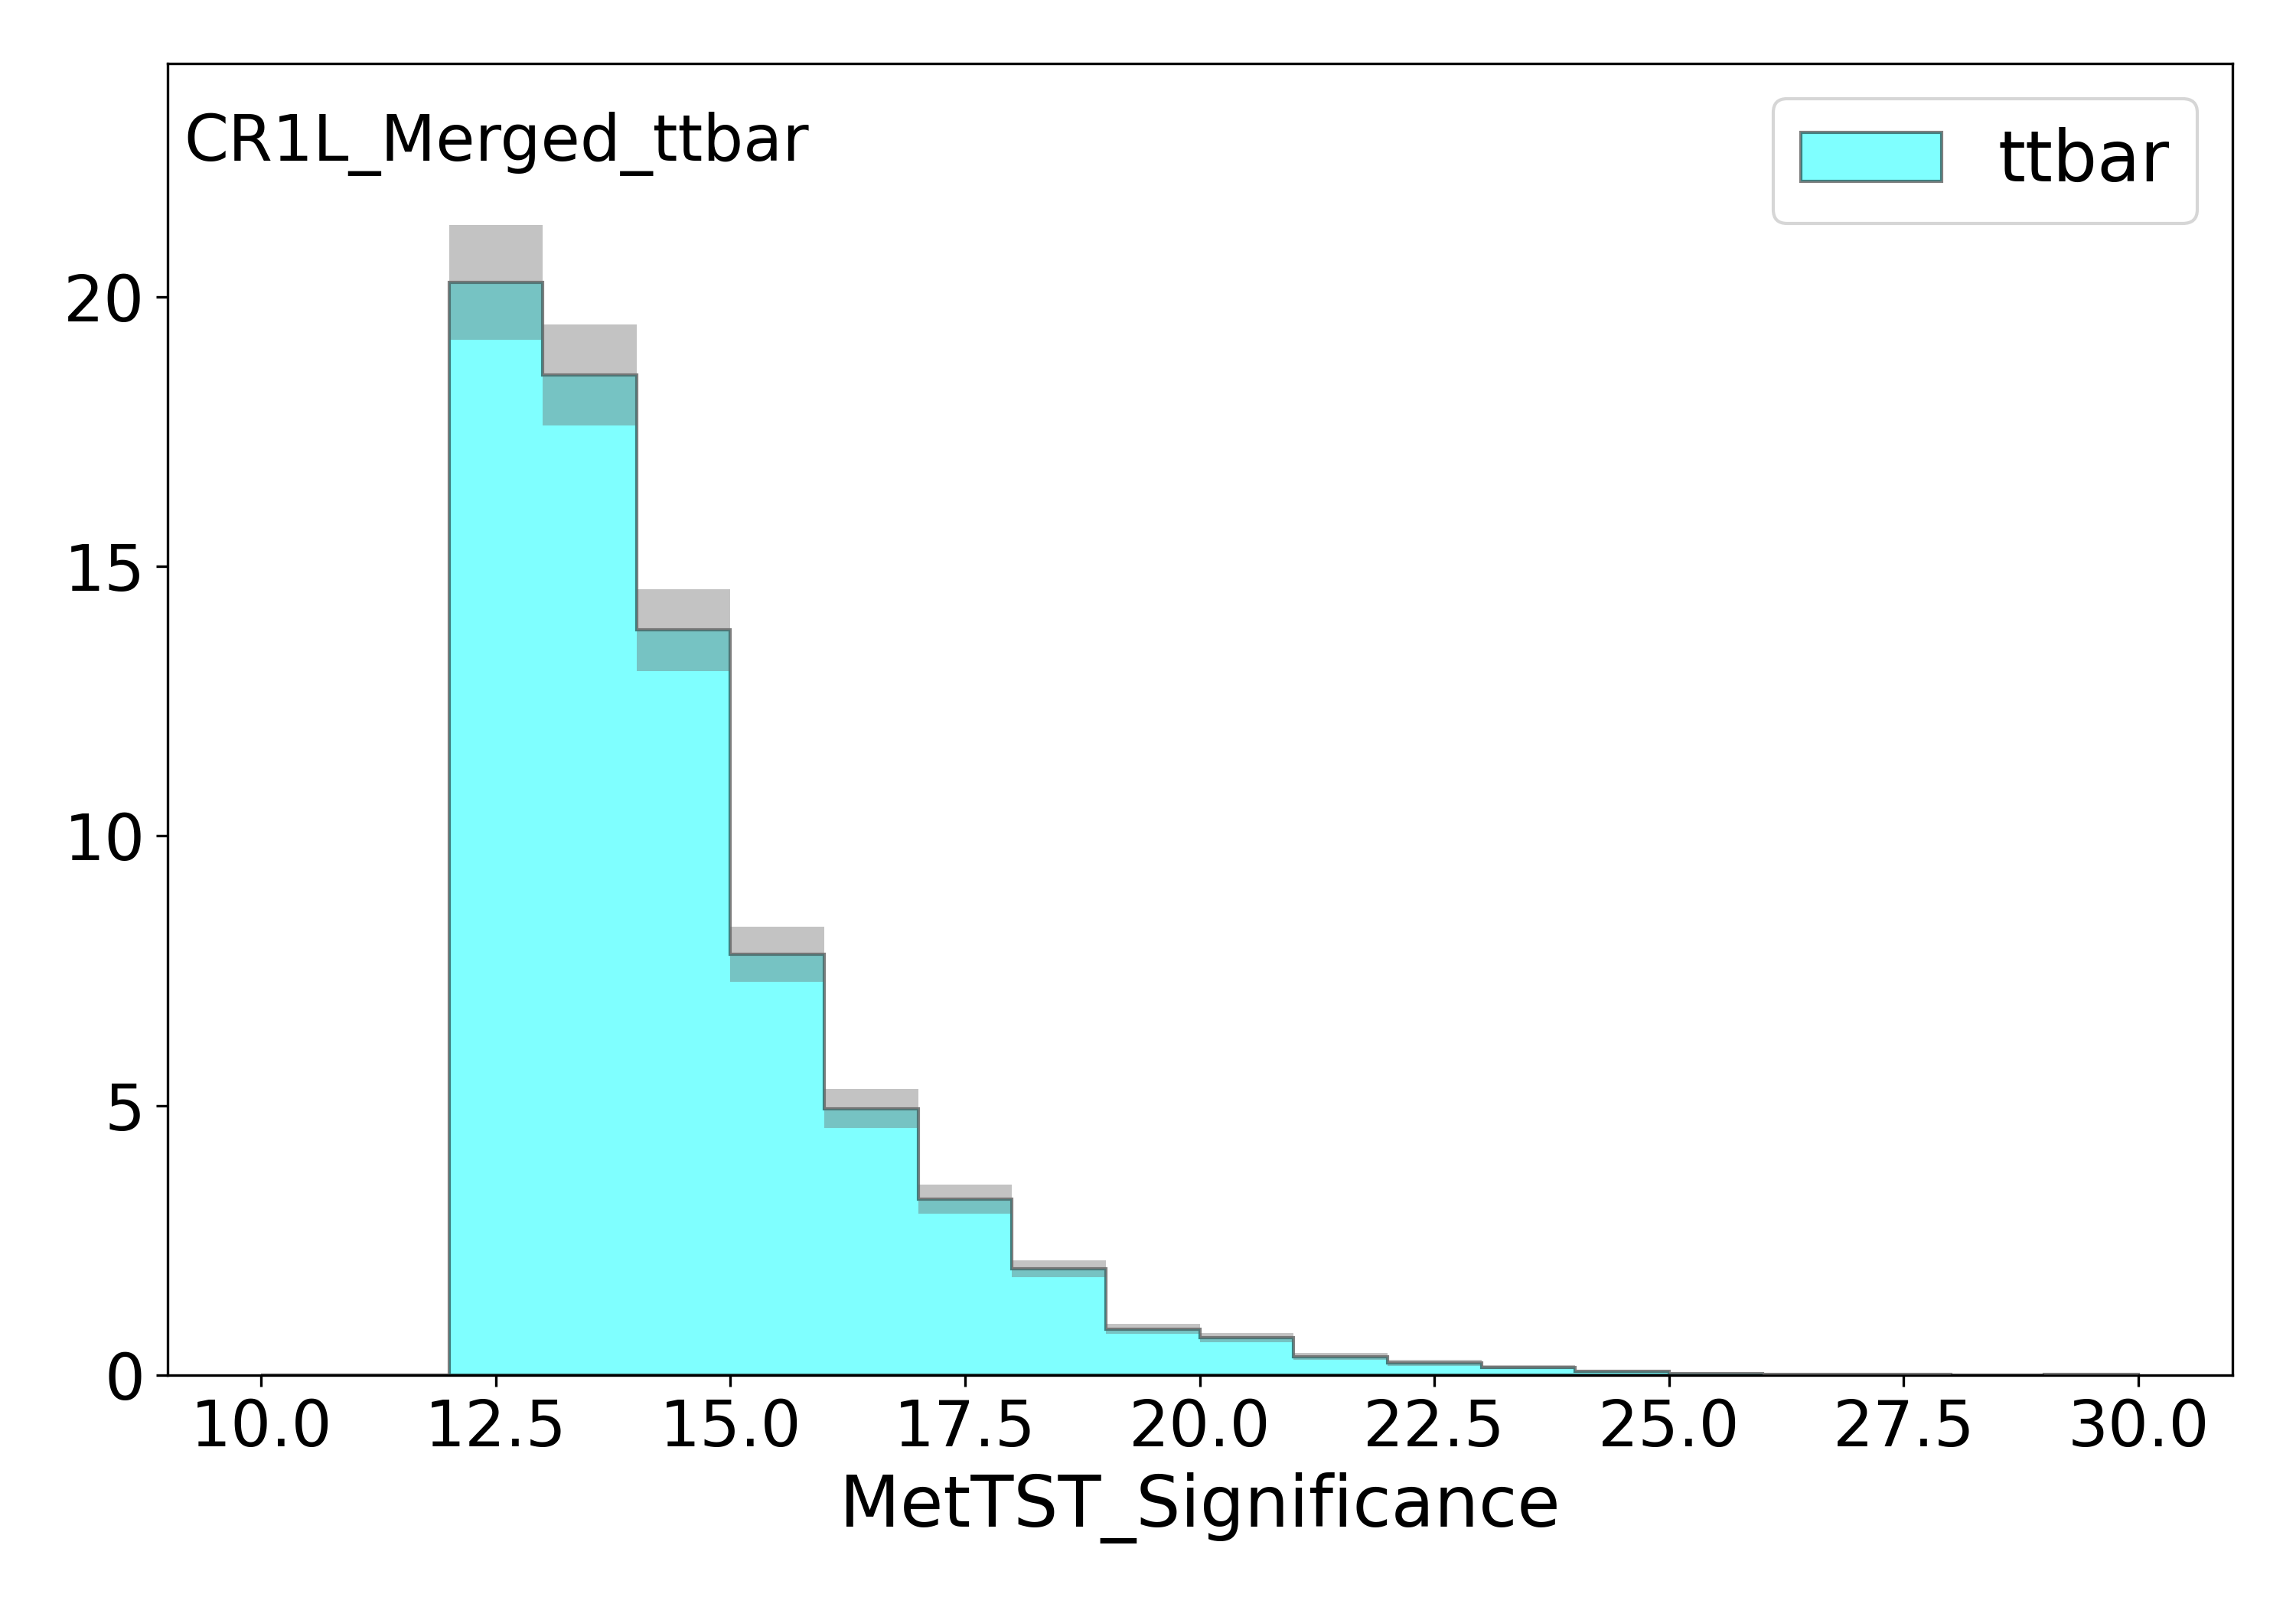
\includegraphics[width = 0.98\textwidth]{Figures/appendix/Preselection/MetTST_Significance.png}
     \caption{\metsig}
     \end{subfigure}
     \caption{Preselection level distribuitions. Grey bands represent MC statistical uncertainty on each bin.}
     \label{fig:Presel1}
  \end{figure}

  \begin{figure}[htbp]
    \centering
     \begin{subfigure}{0.49\textwidth}
     \includegraphics[width = 0.98\textwidth]{Figures/appendix/Preselection/dR_lep_TARJets10.png}
     \caption{\drTARl}
     \end{subfigure}
     \begin{subfigure}{0.49\textwidth}
     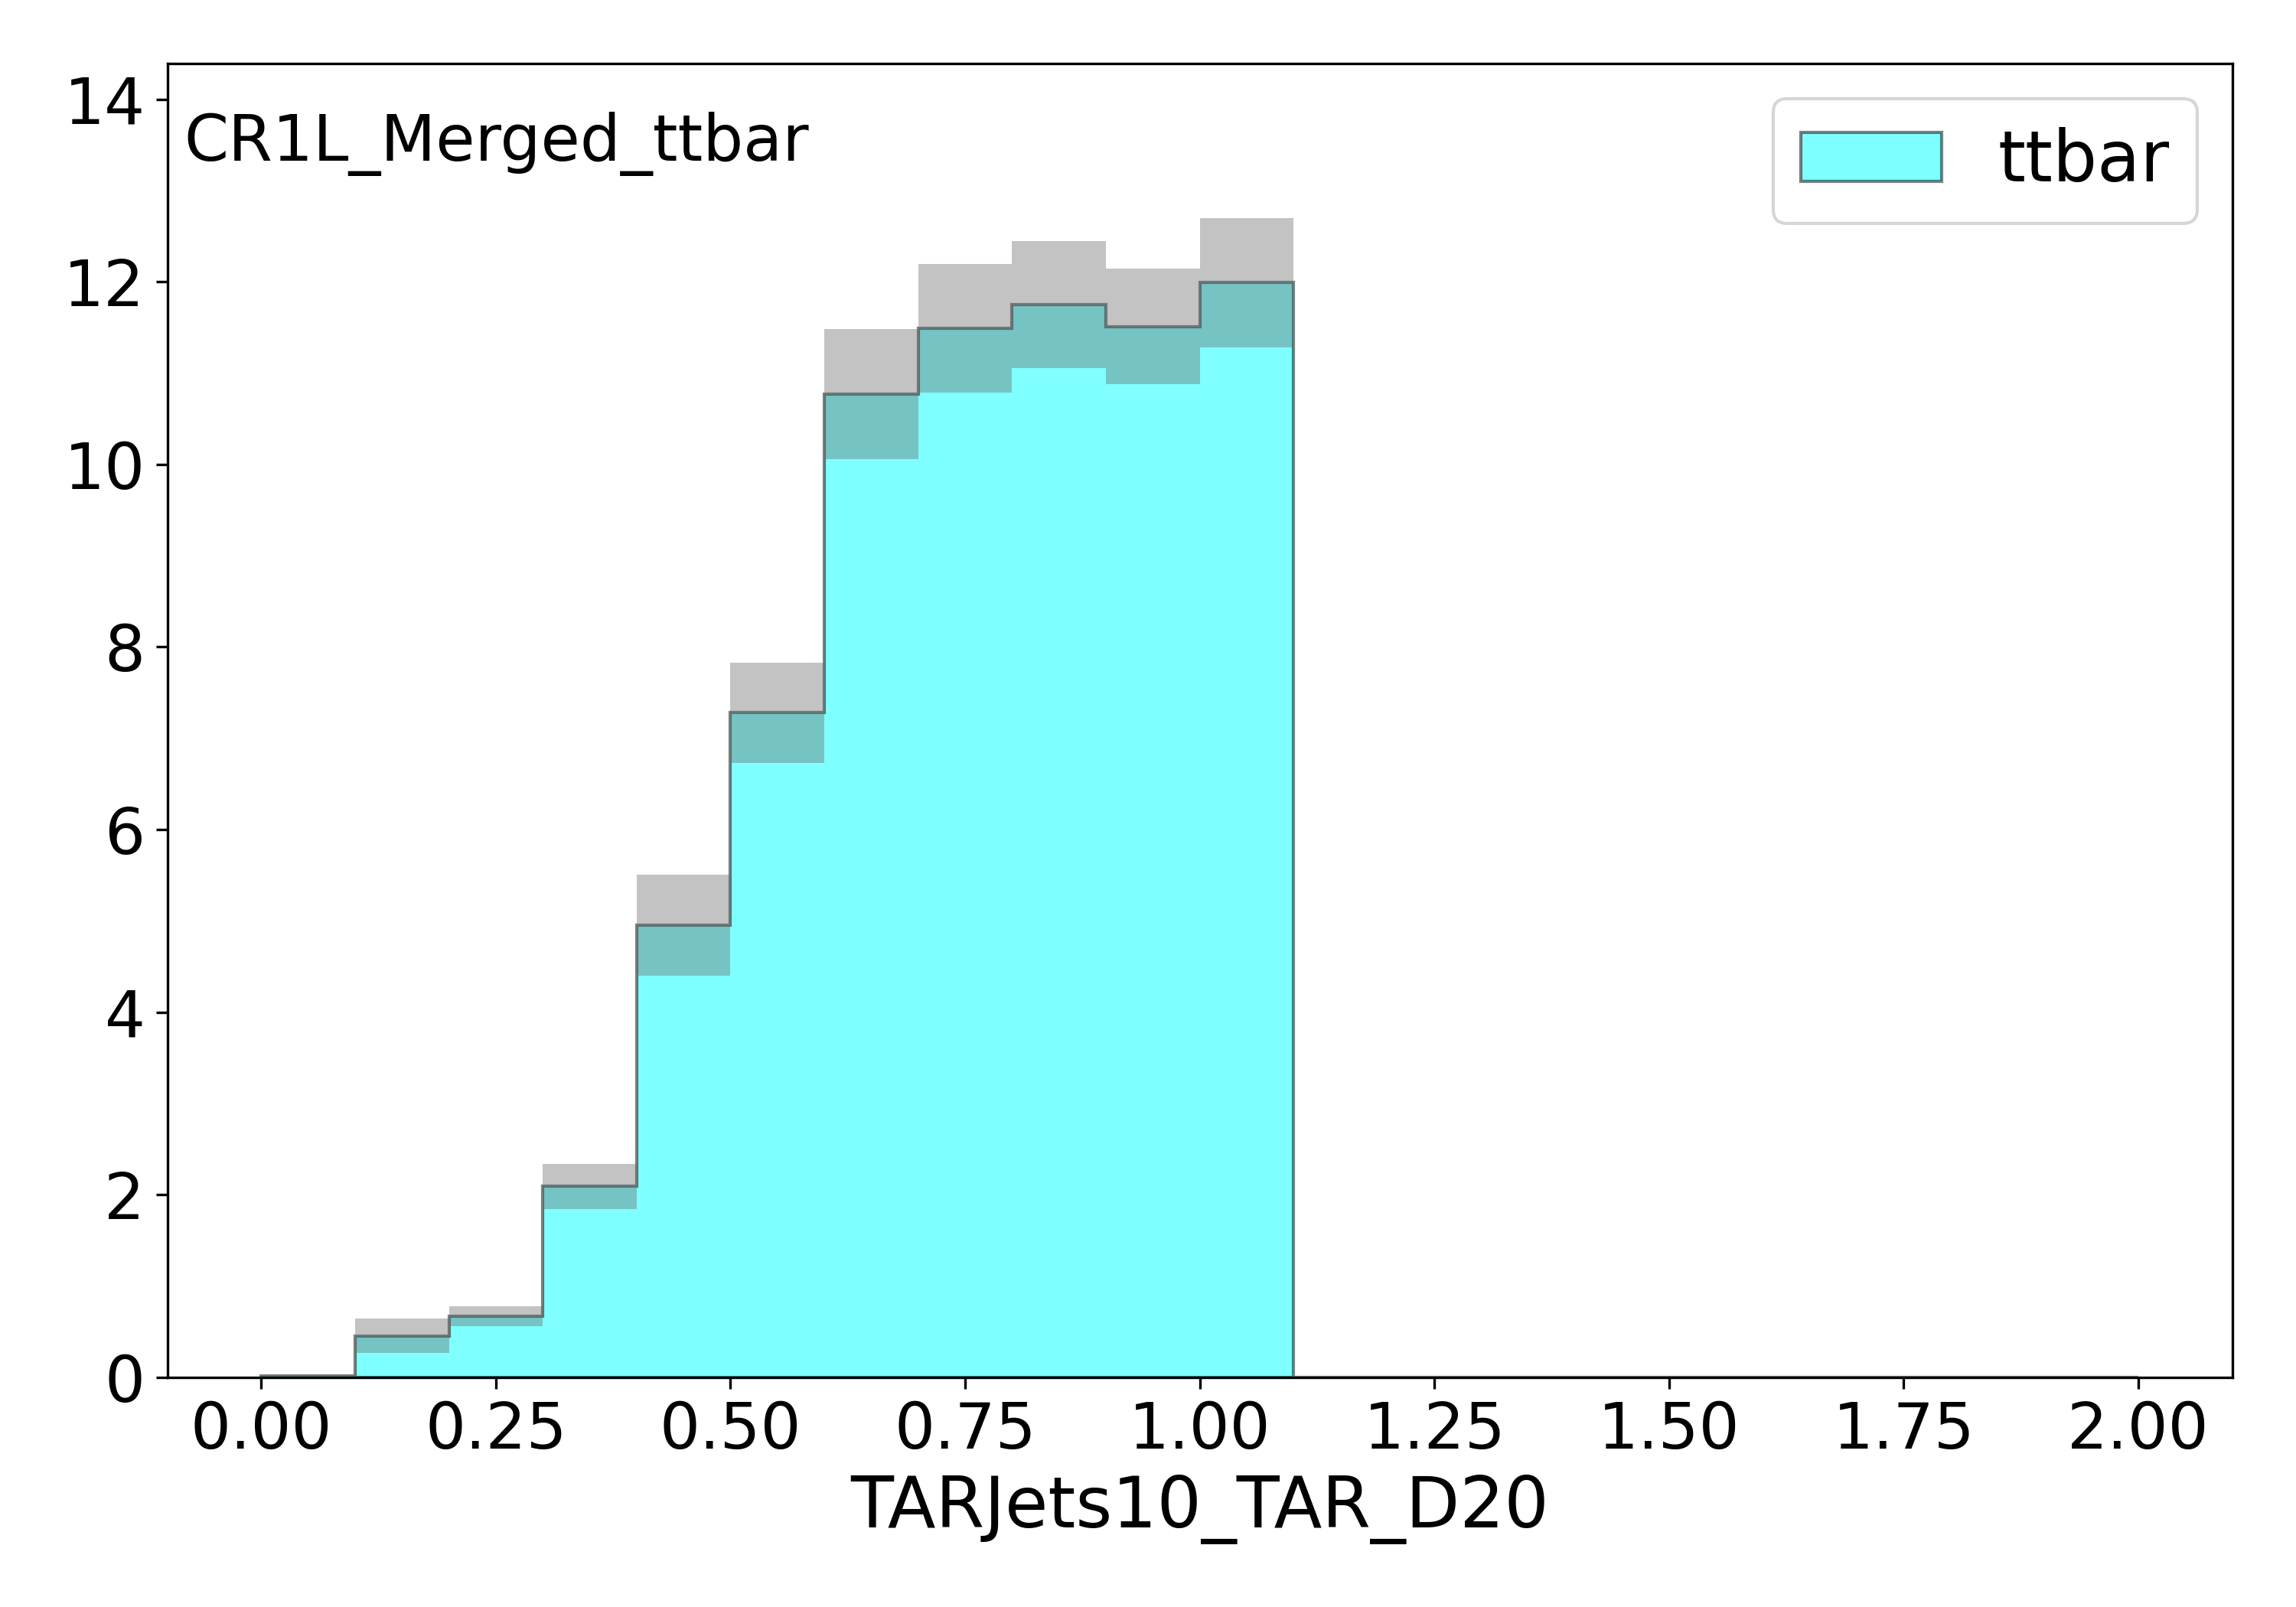
\includegraphics[width = 0.98\textwidth]{Figures/appendix/Preselection/TARJets10_TAR_D20.png}
     \caption{\DtwoTAR}
     \end{subfigure}
     \begin{subfigure}{0.49\textwidth}
     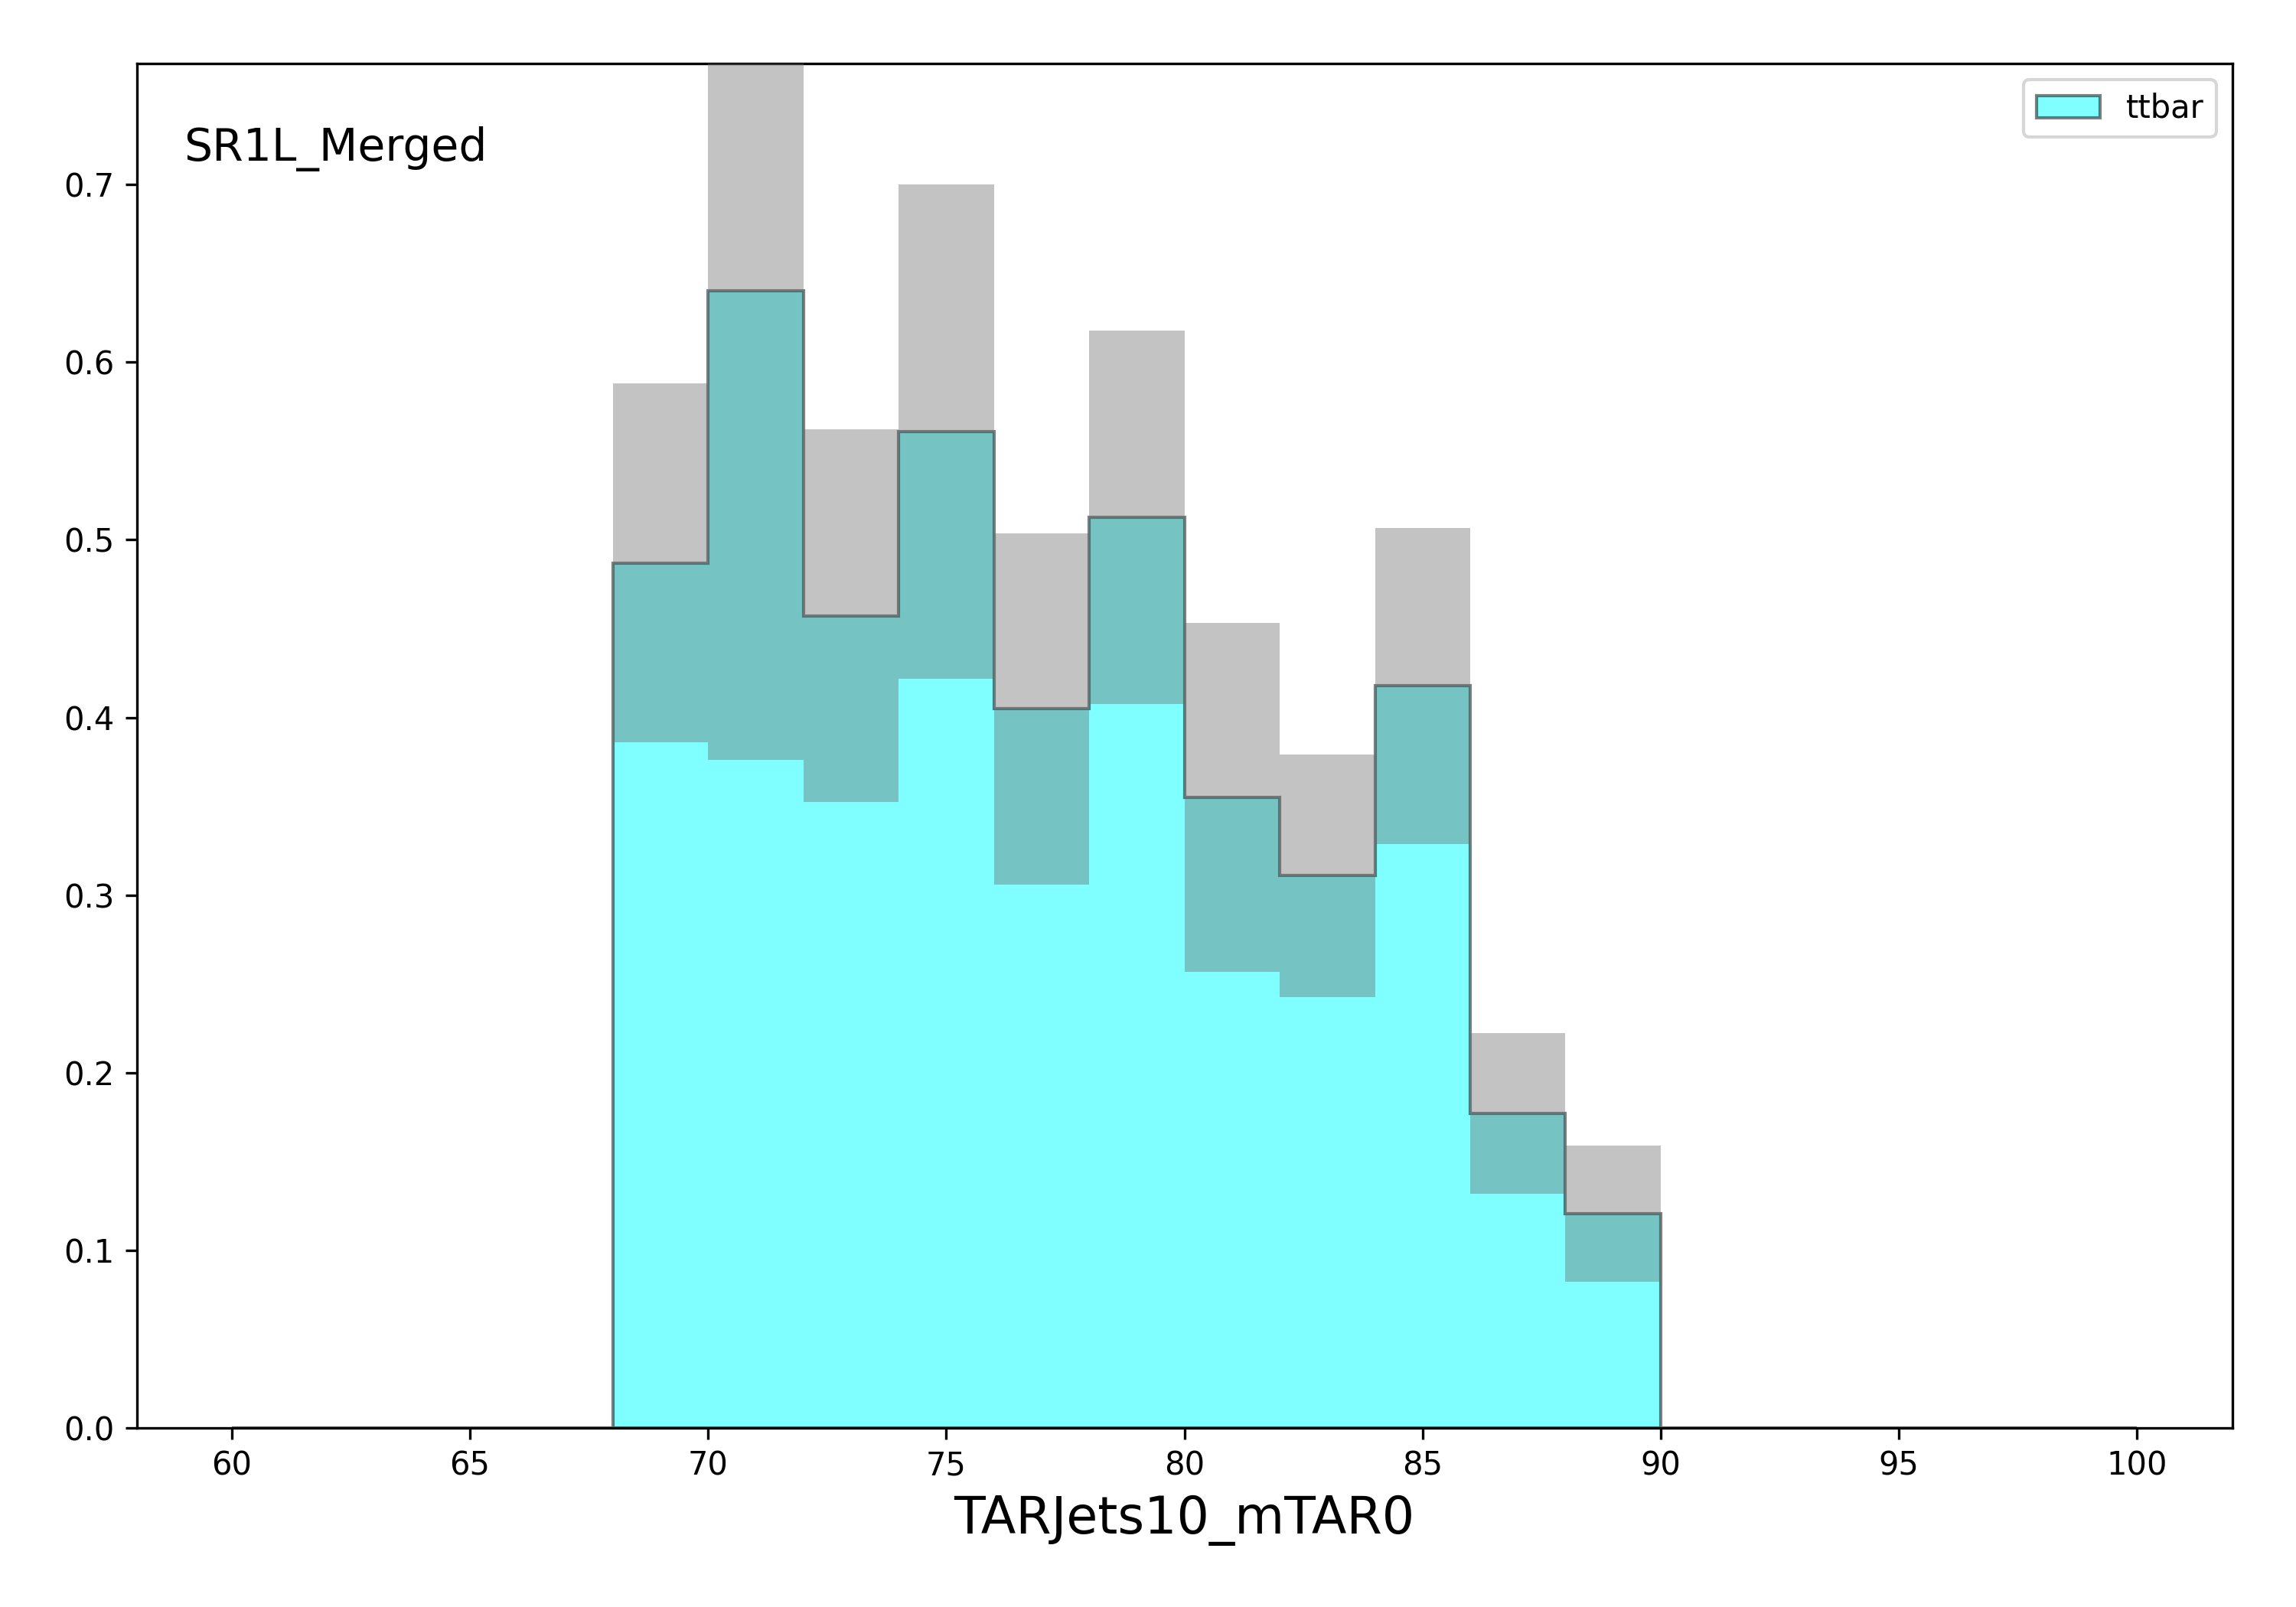
\includegraphics[width = 0.98\textwidth]{Figures/appendix/Preselection/TARJets10_mTAR0.png}
     \caption{\mTAR}
     \end{subfigure}
     \begin{subfigure}{0.49\textwidth}
     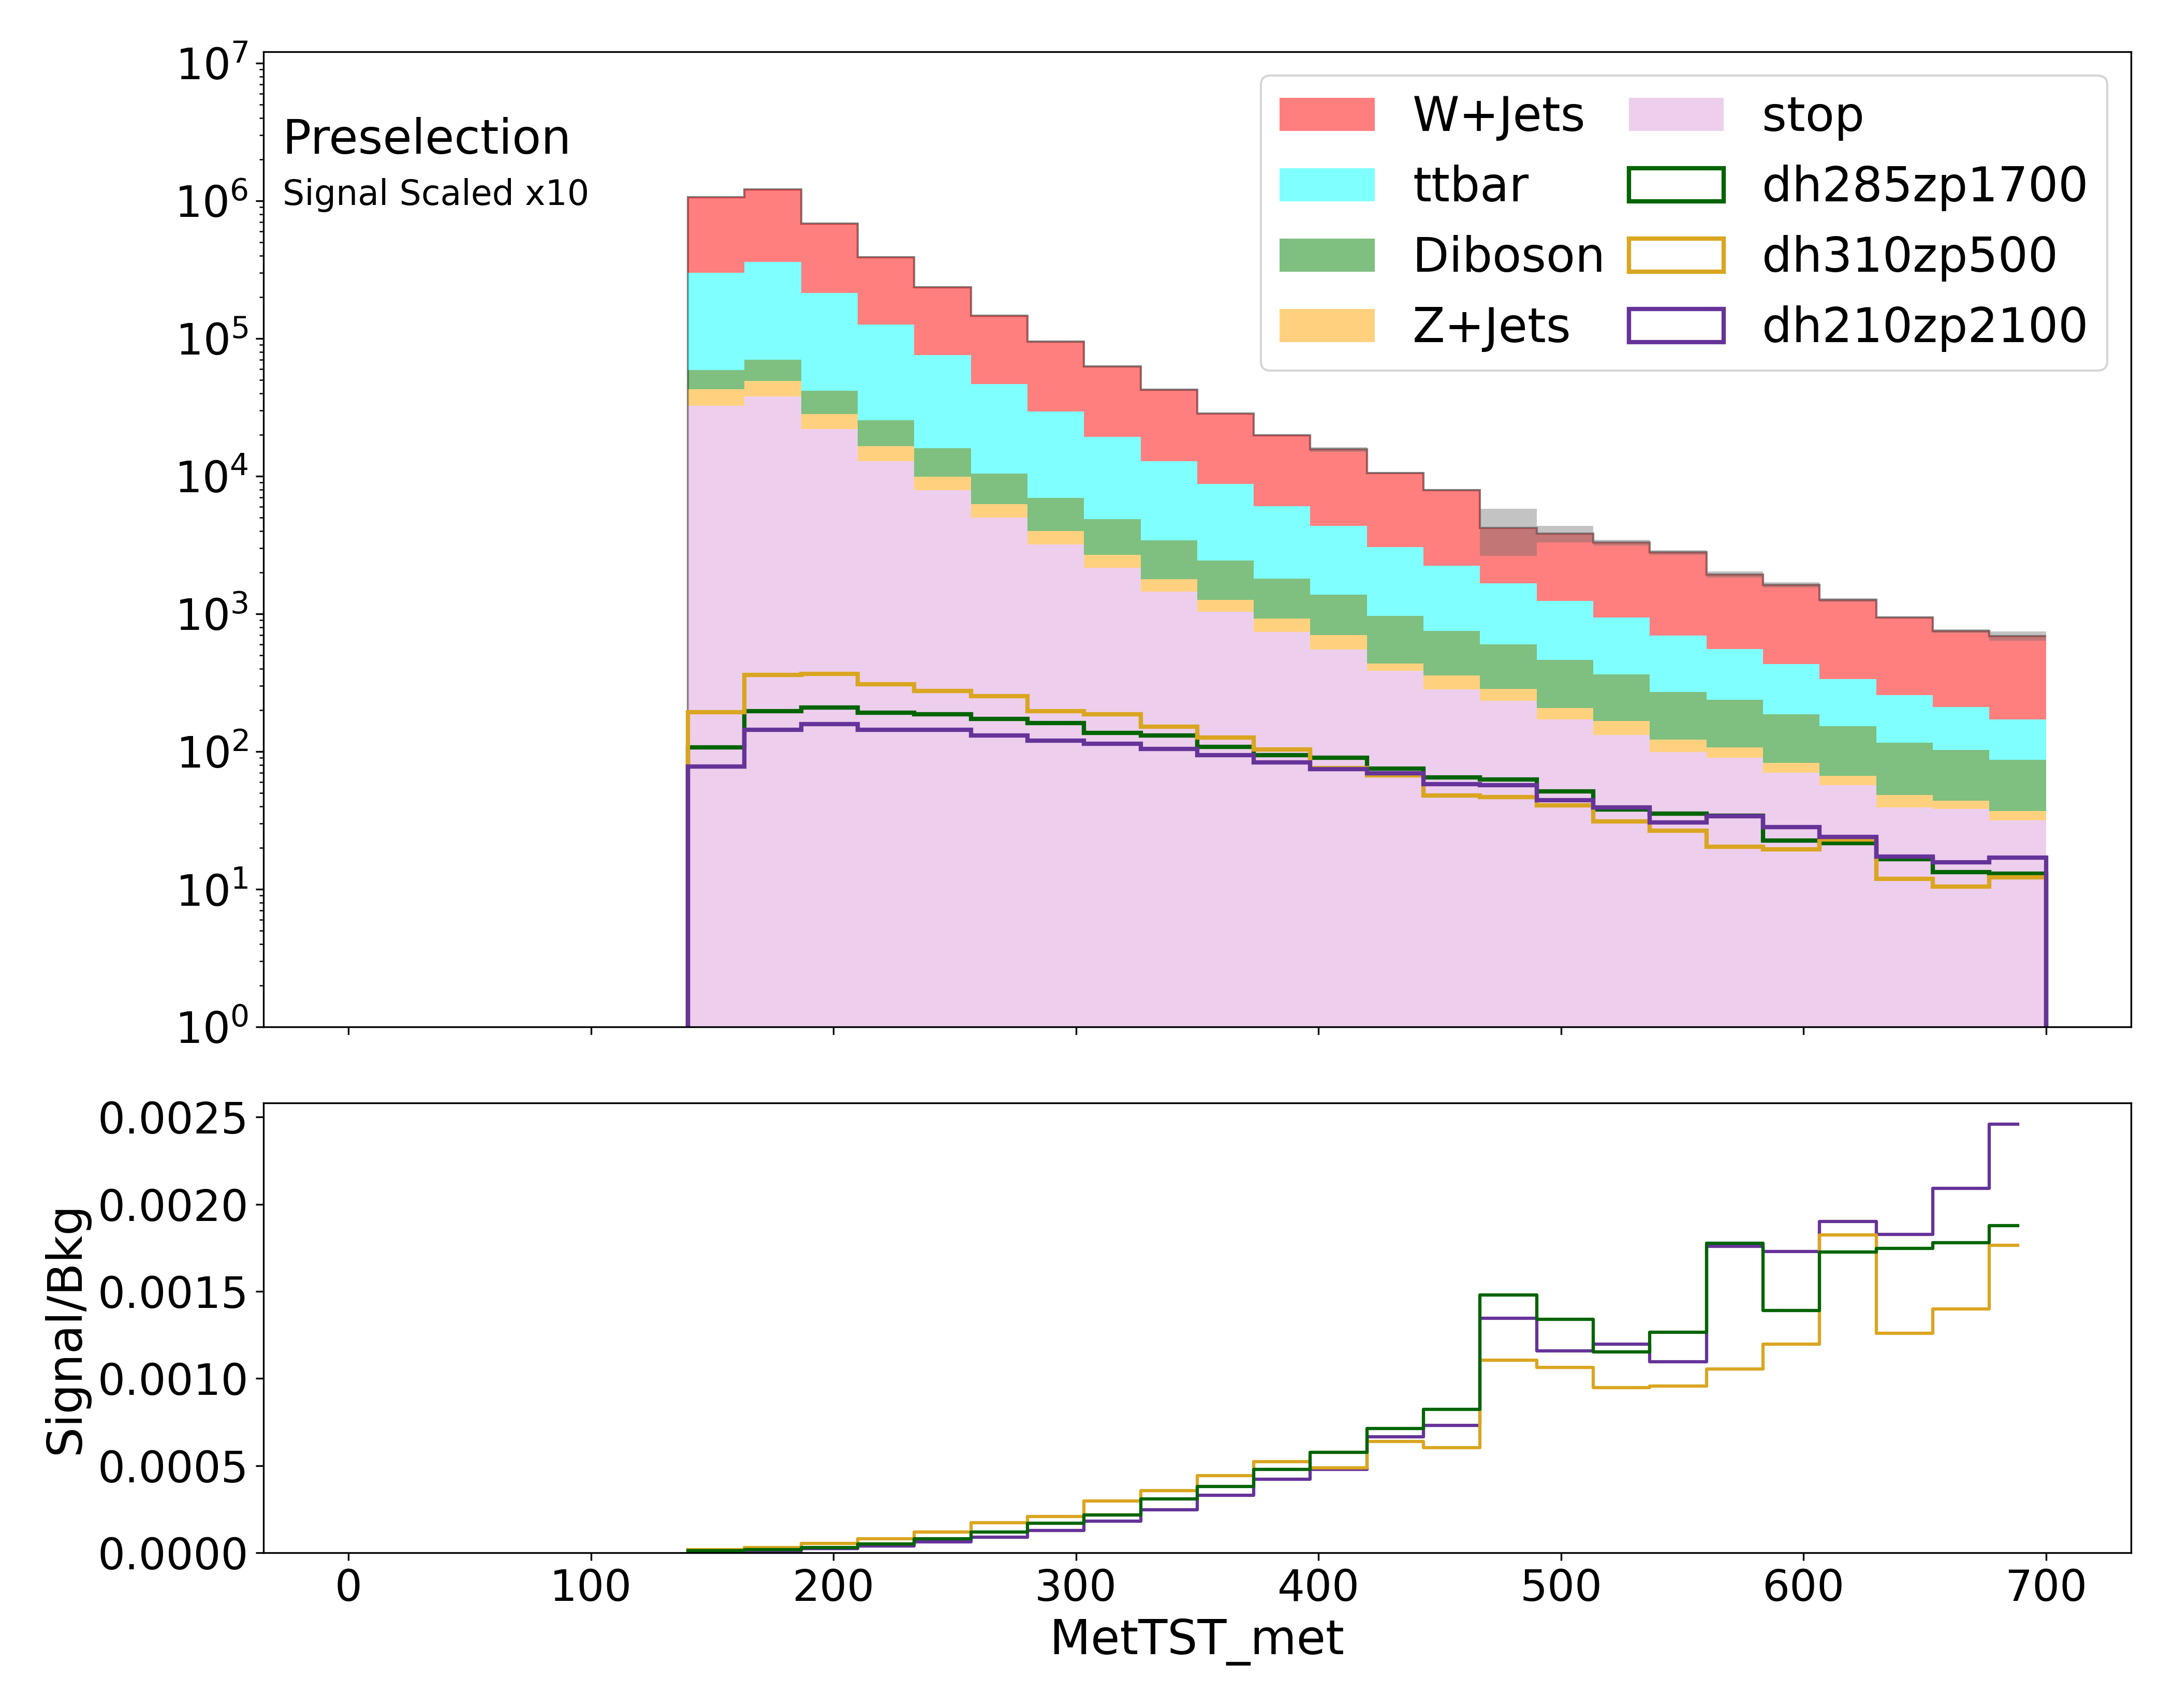
\includegraphics[width = 0.98\textwidth]{Figures/appendix/Preselection/MetTST_met.png}
     \caption{\met}
     \end{subfigure}
     \caption{Preselection level distribuitions. Grey bands represent MC statistical uncertainty on each bin.}
     \label{fig:Presel1}
  \end{figure}

  \begin{figure}[htbp]
    \centering
      \begin{subfigure}{0.49\textwidth}
      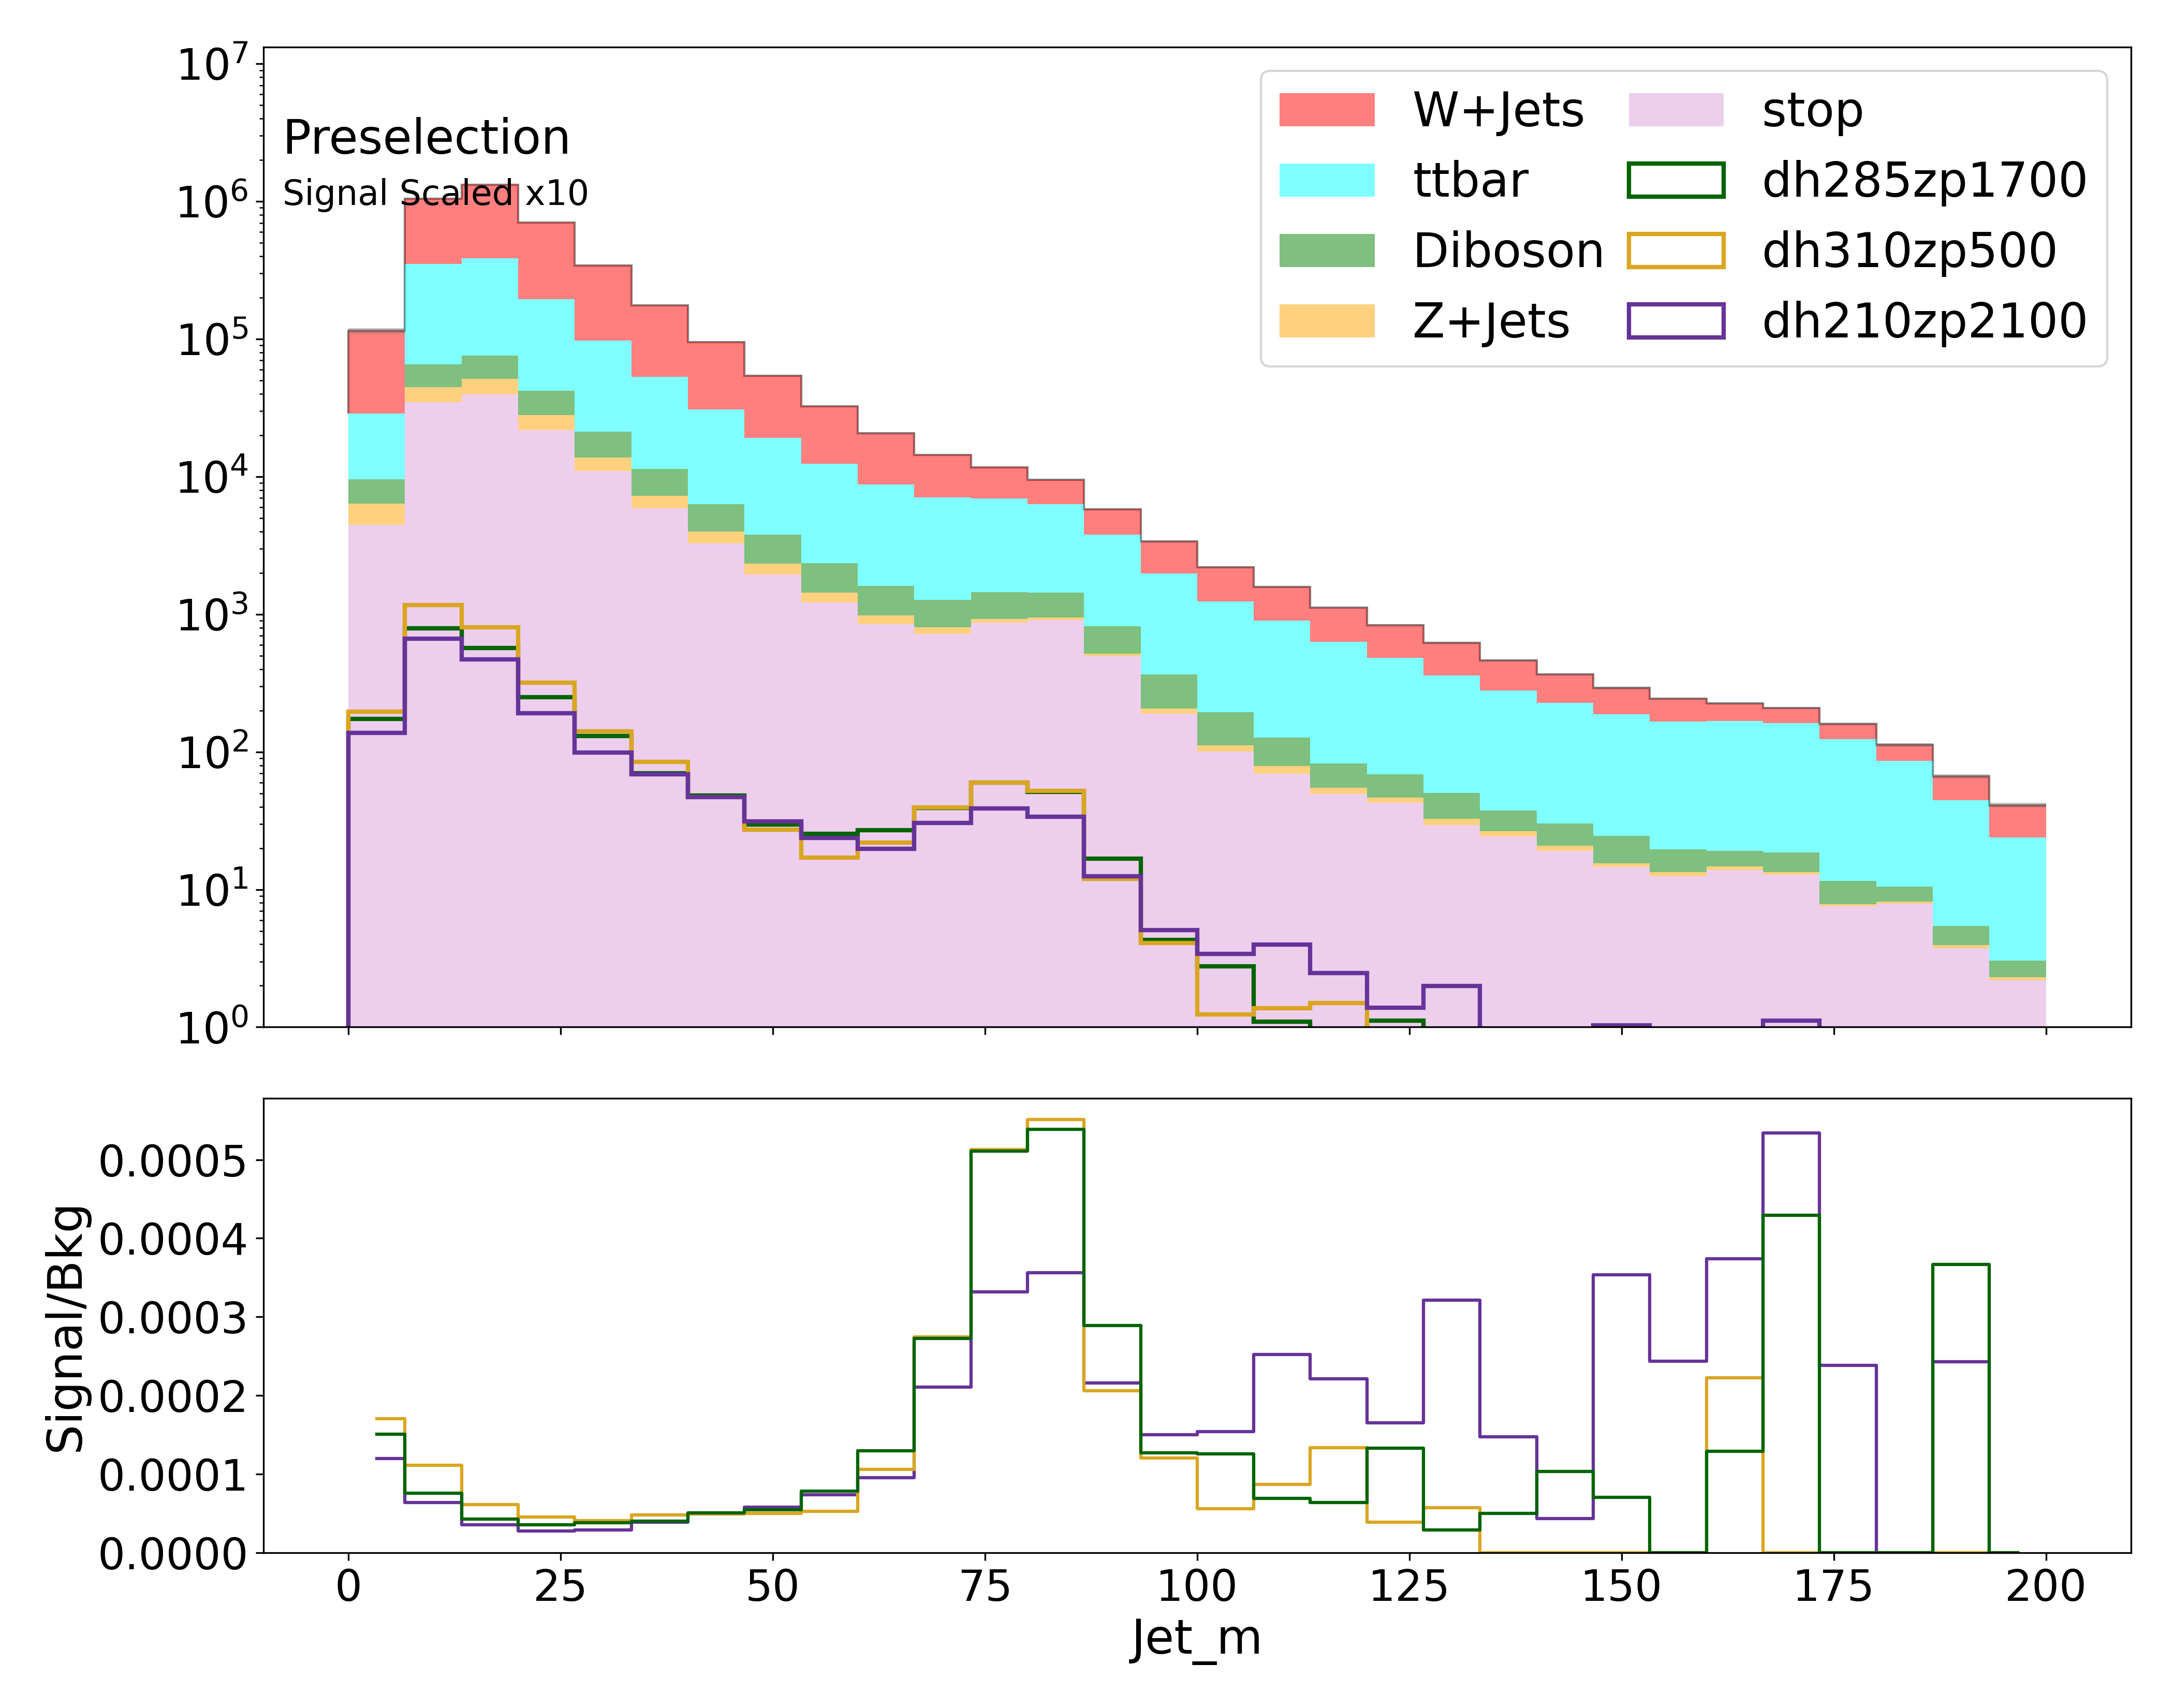
\includegraphics[width = 0.98\textwidth]{Figures/appendix/Preselection/Jet_m.png}
      \caption{\ensuremath{m_{\text{Jet}}}}
      \end{subfigure}
      \begin{subfigure}{0.49\textwidth}
      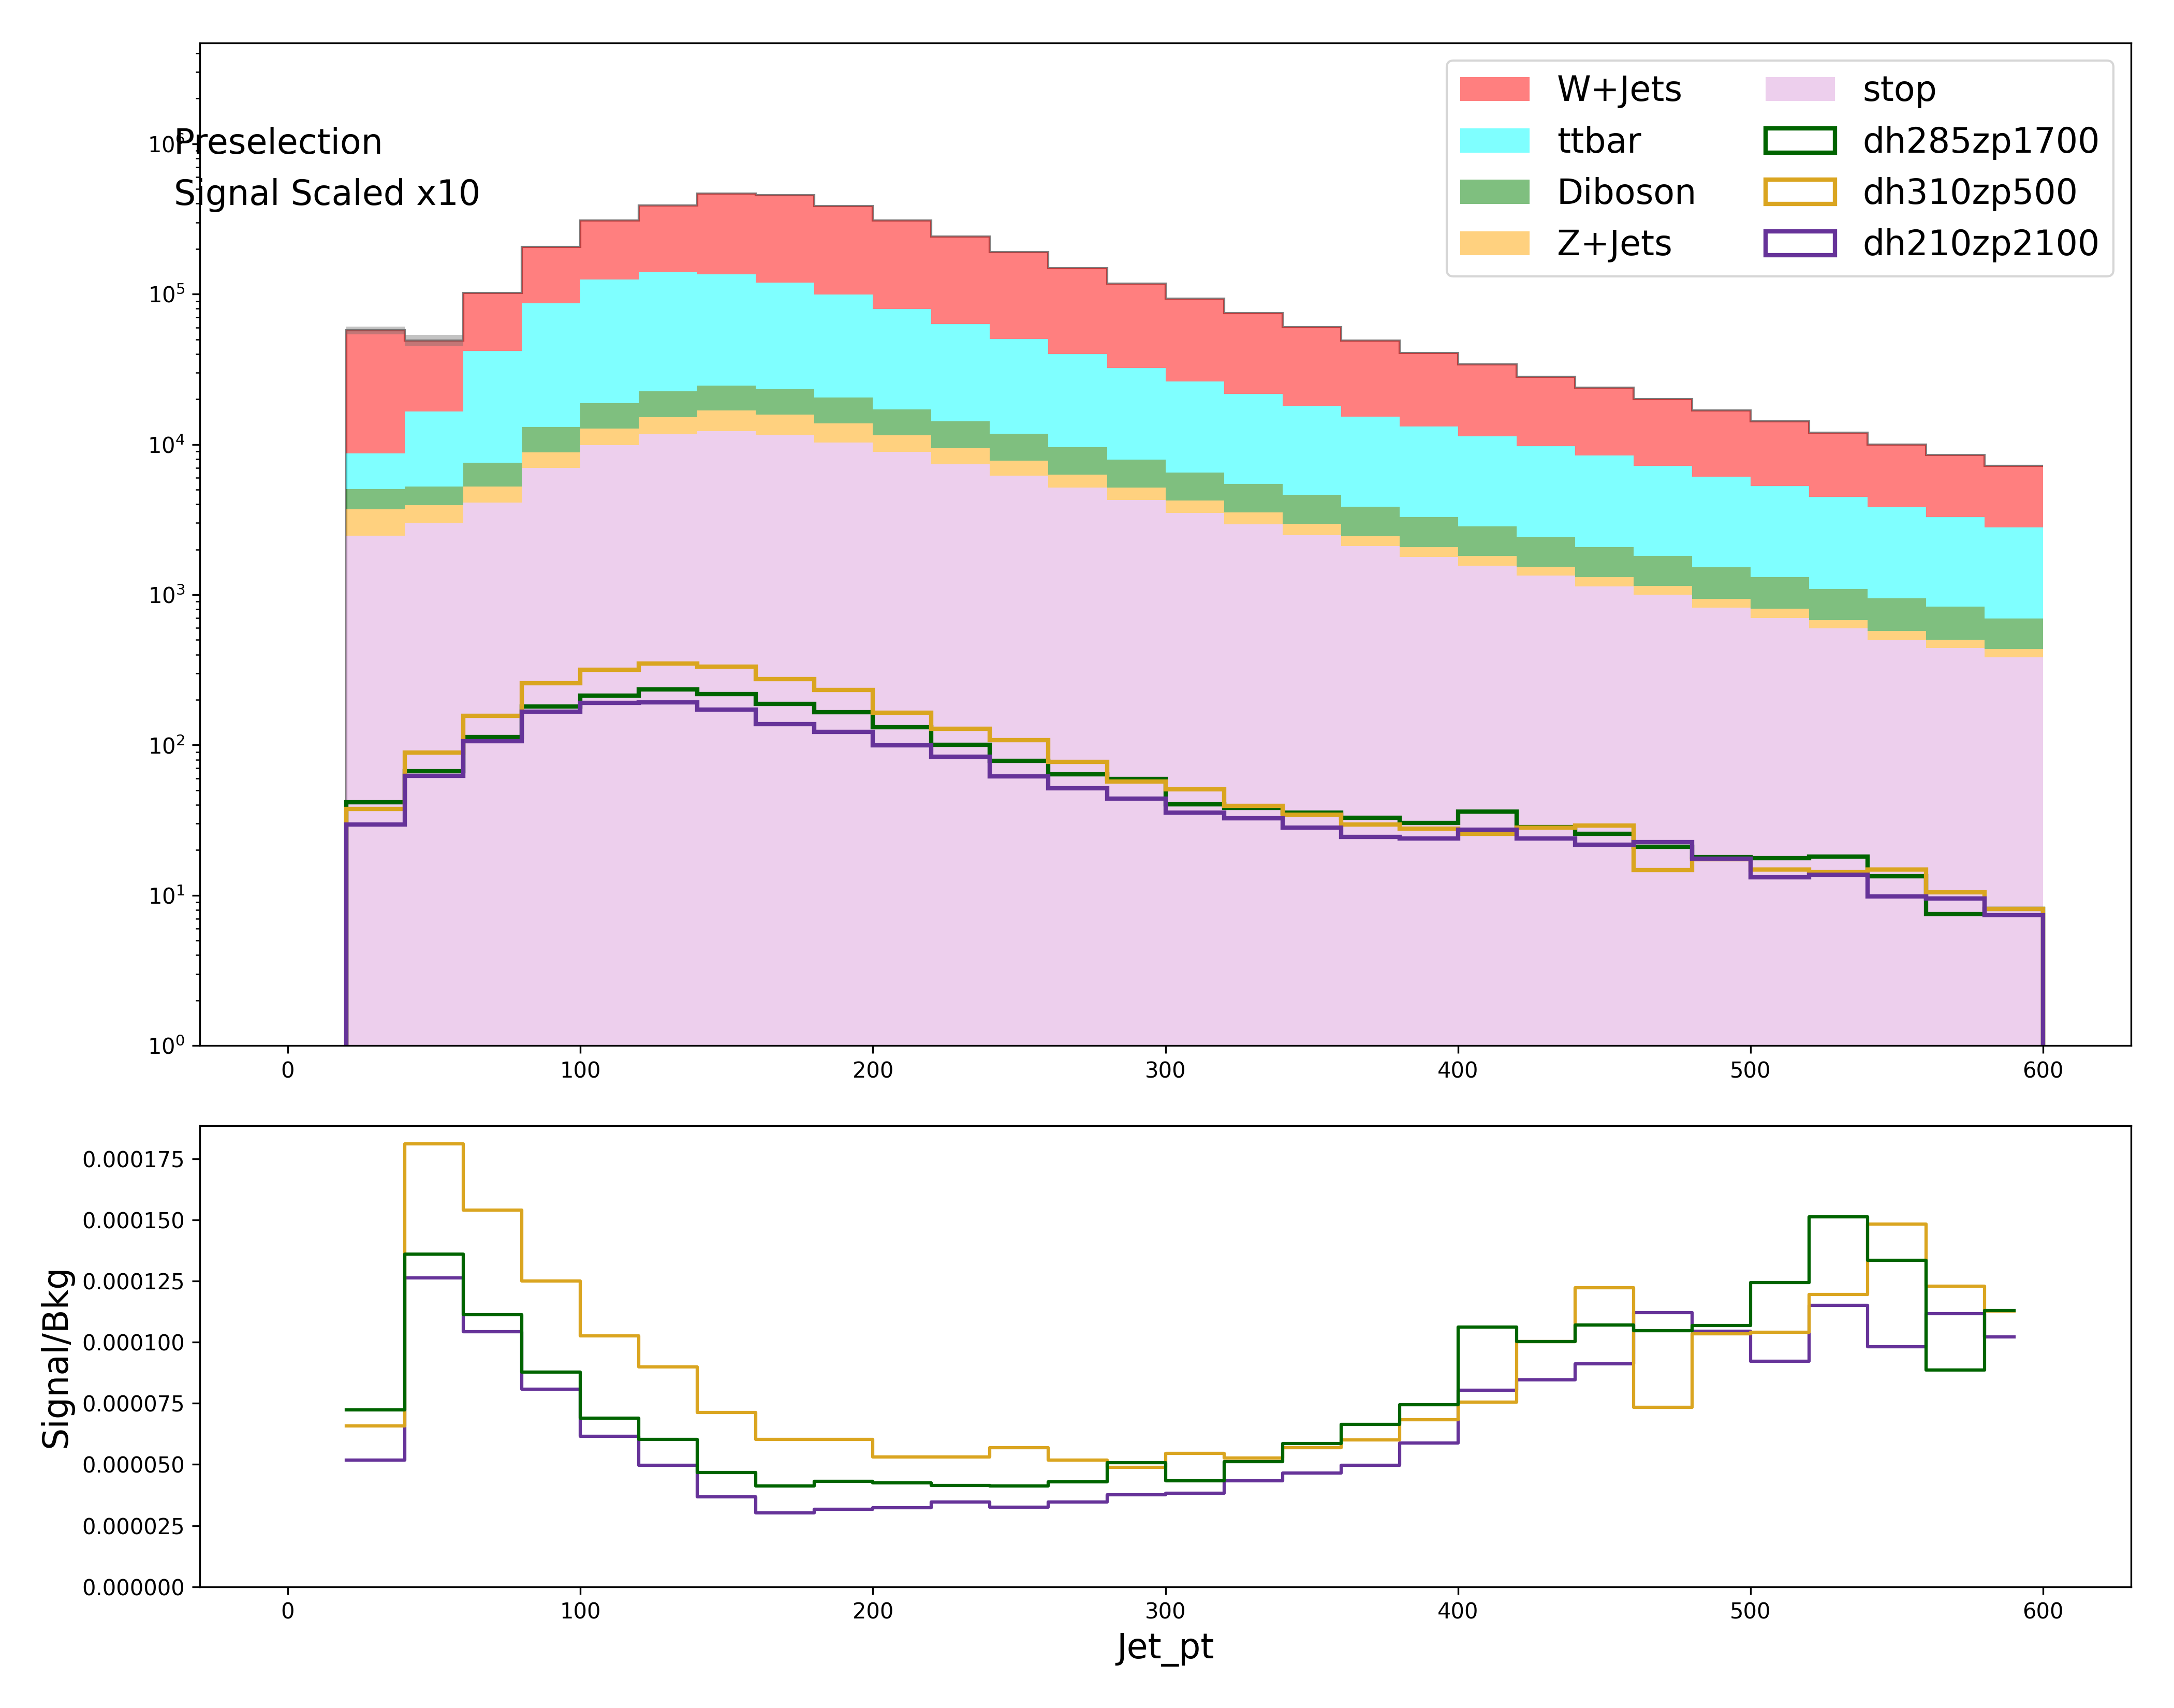
\includegraphics[width = 0.98\textwidth]{Figures/appendix/Preselection/Jet_pt.png}
      \caption{\ensuremath{\pT(\text{Jet})}}
      \end{subfigure}
      \begin{subfigure}{0.49\textwidth}
      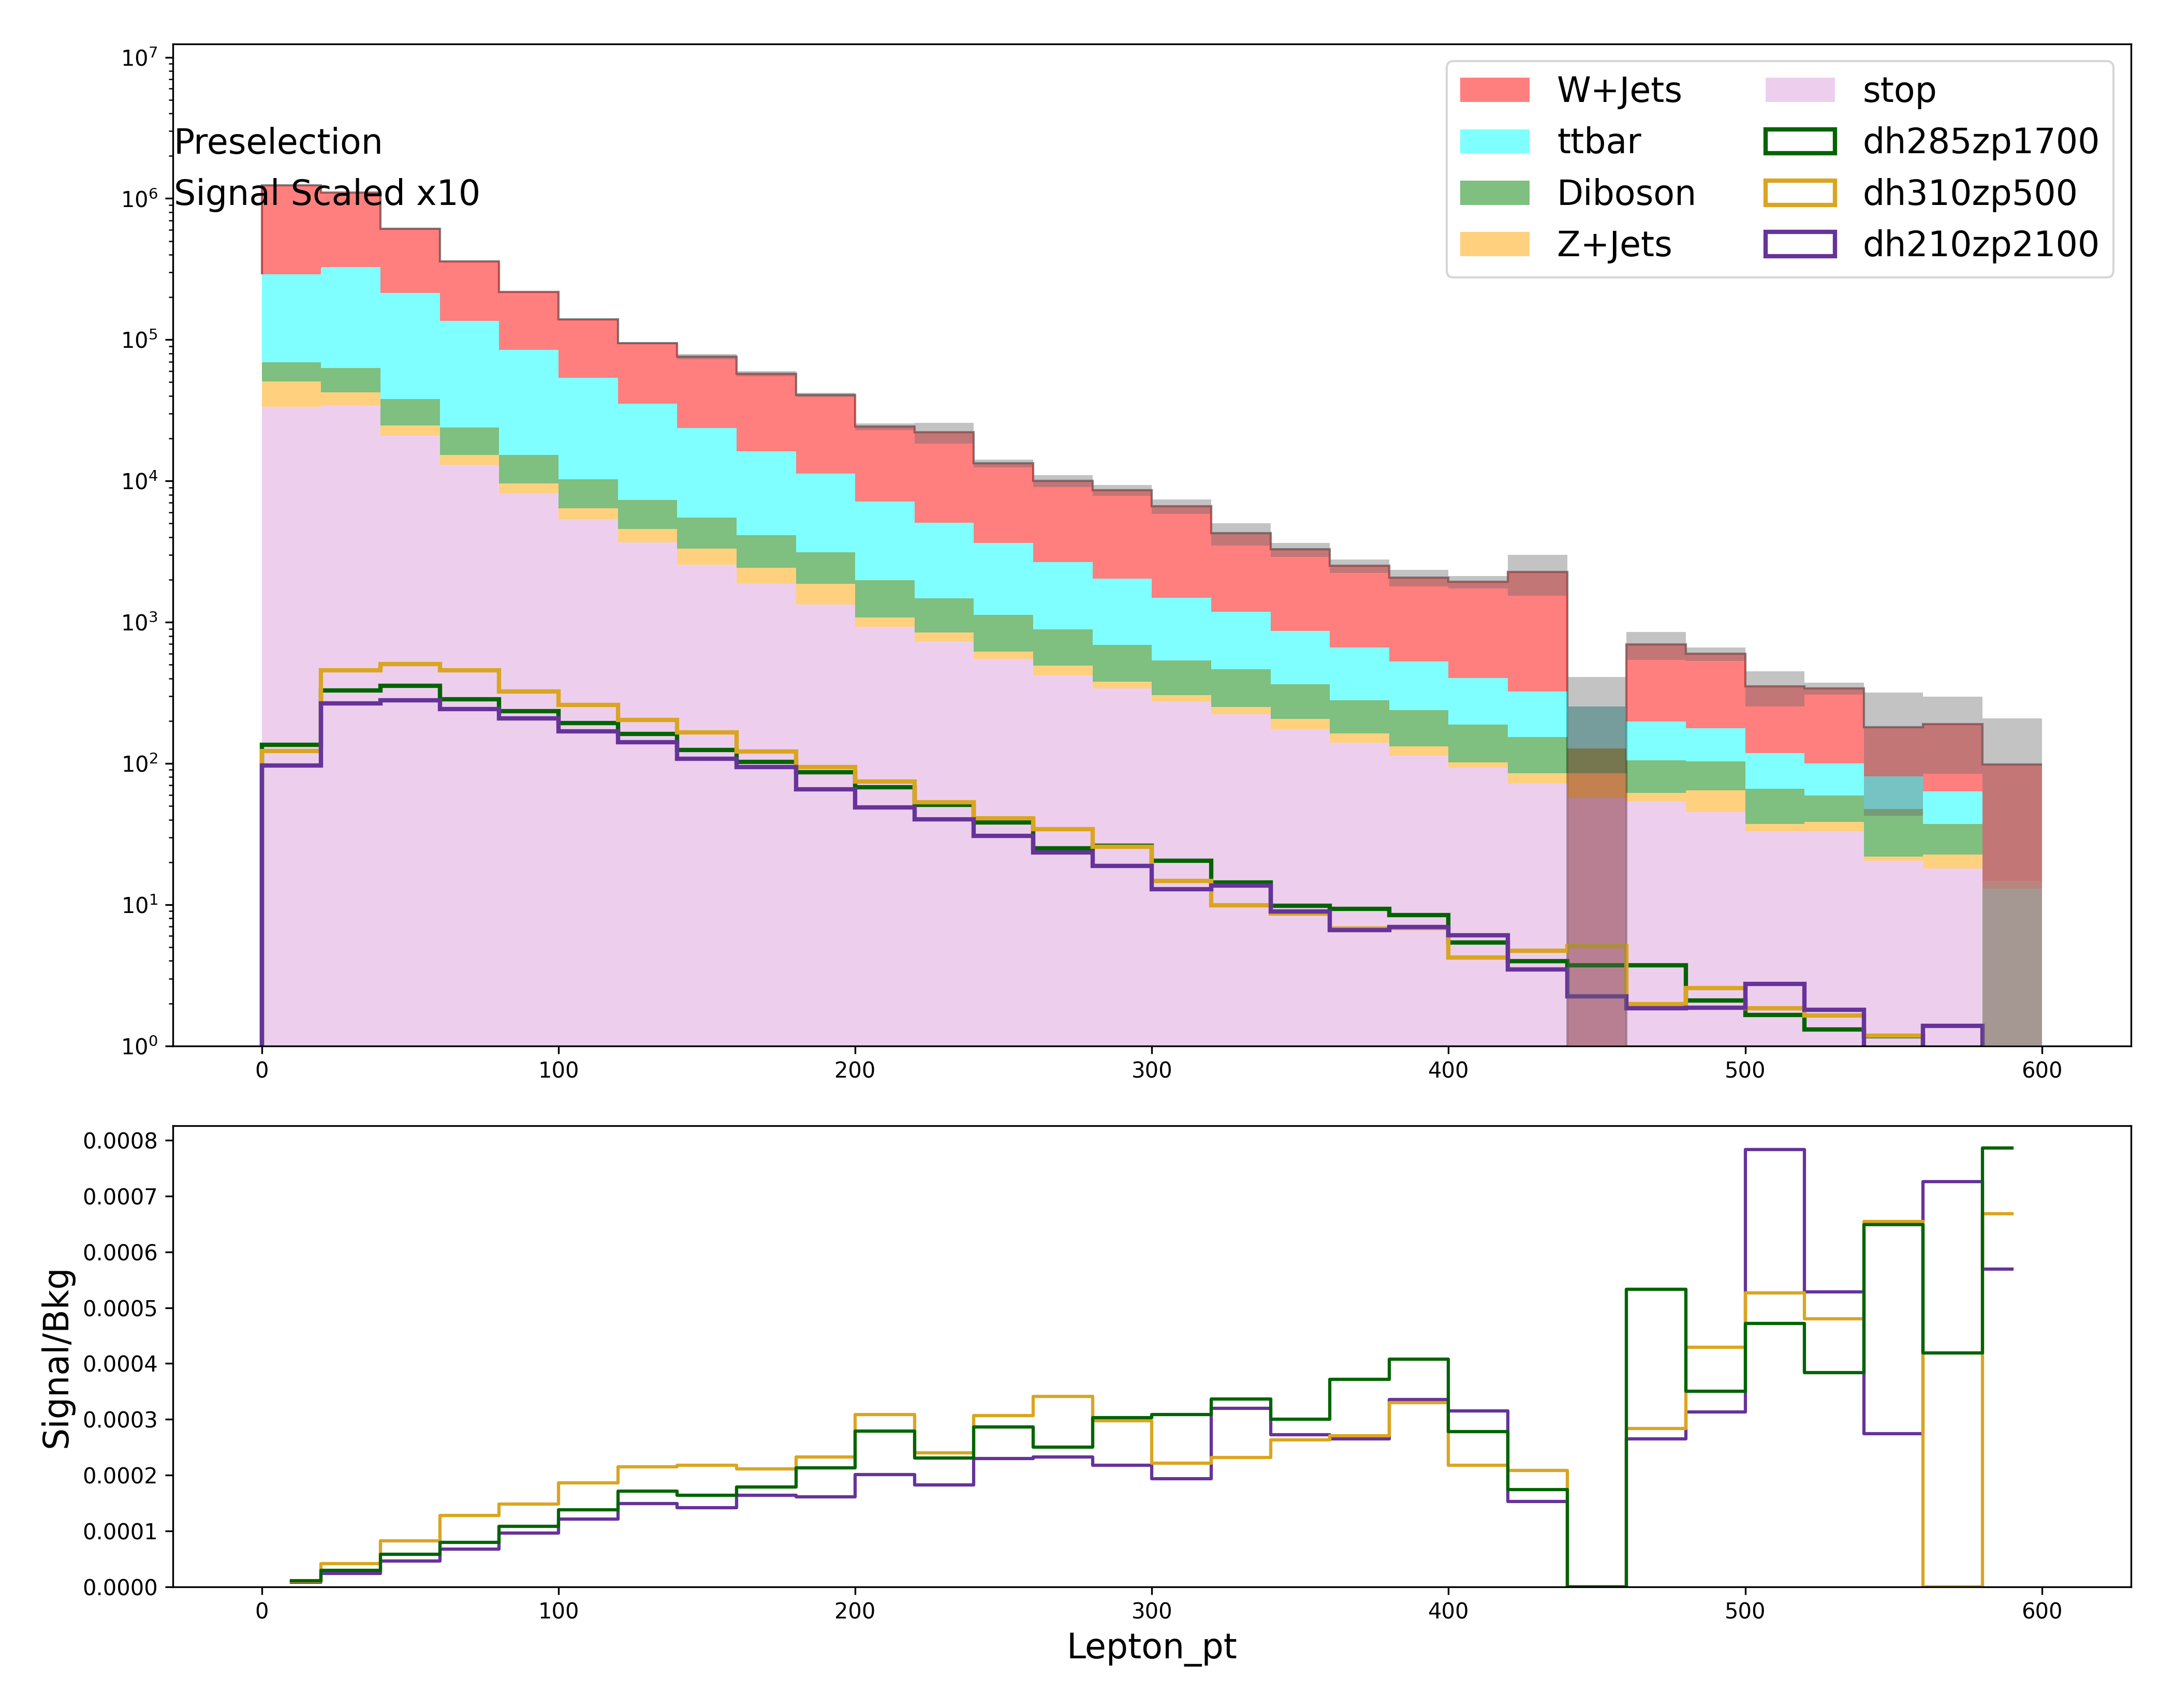
\includegraphics[width = 0.98\textwidth]{Figures/appendix/Preselection/Lepton_pt.png}
      \caption{$\pT(\ell)$}
      \end{subfigure}
      \begin{subfigure}{0.49\textwidth}
      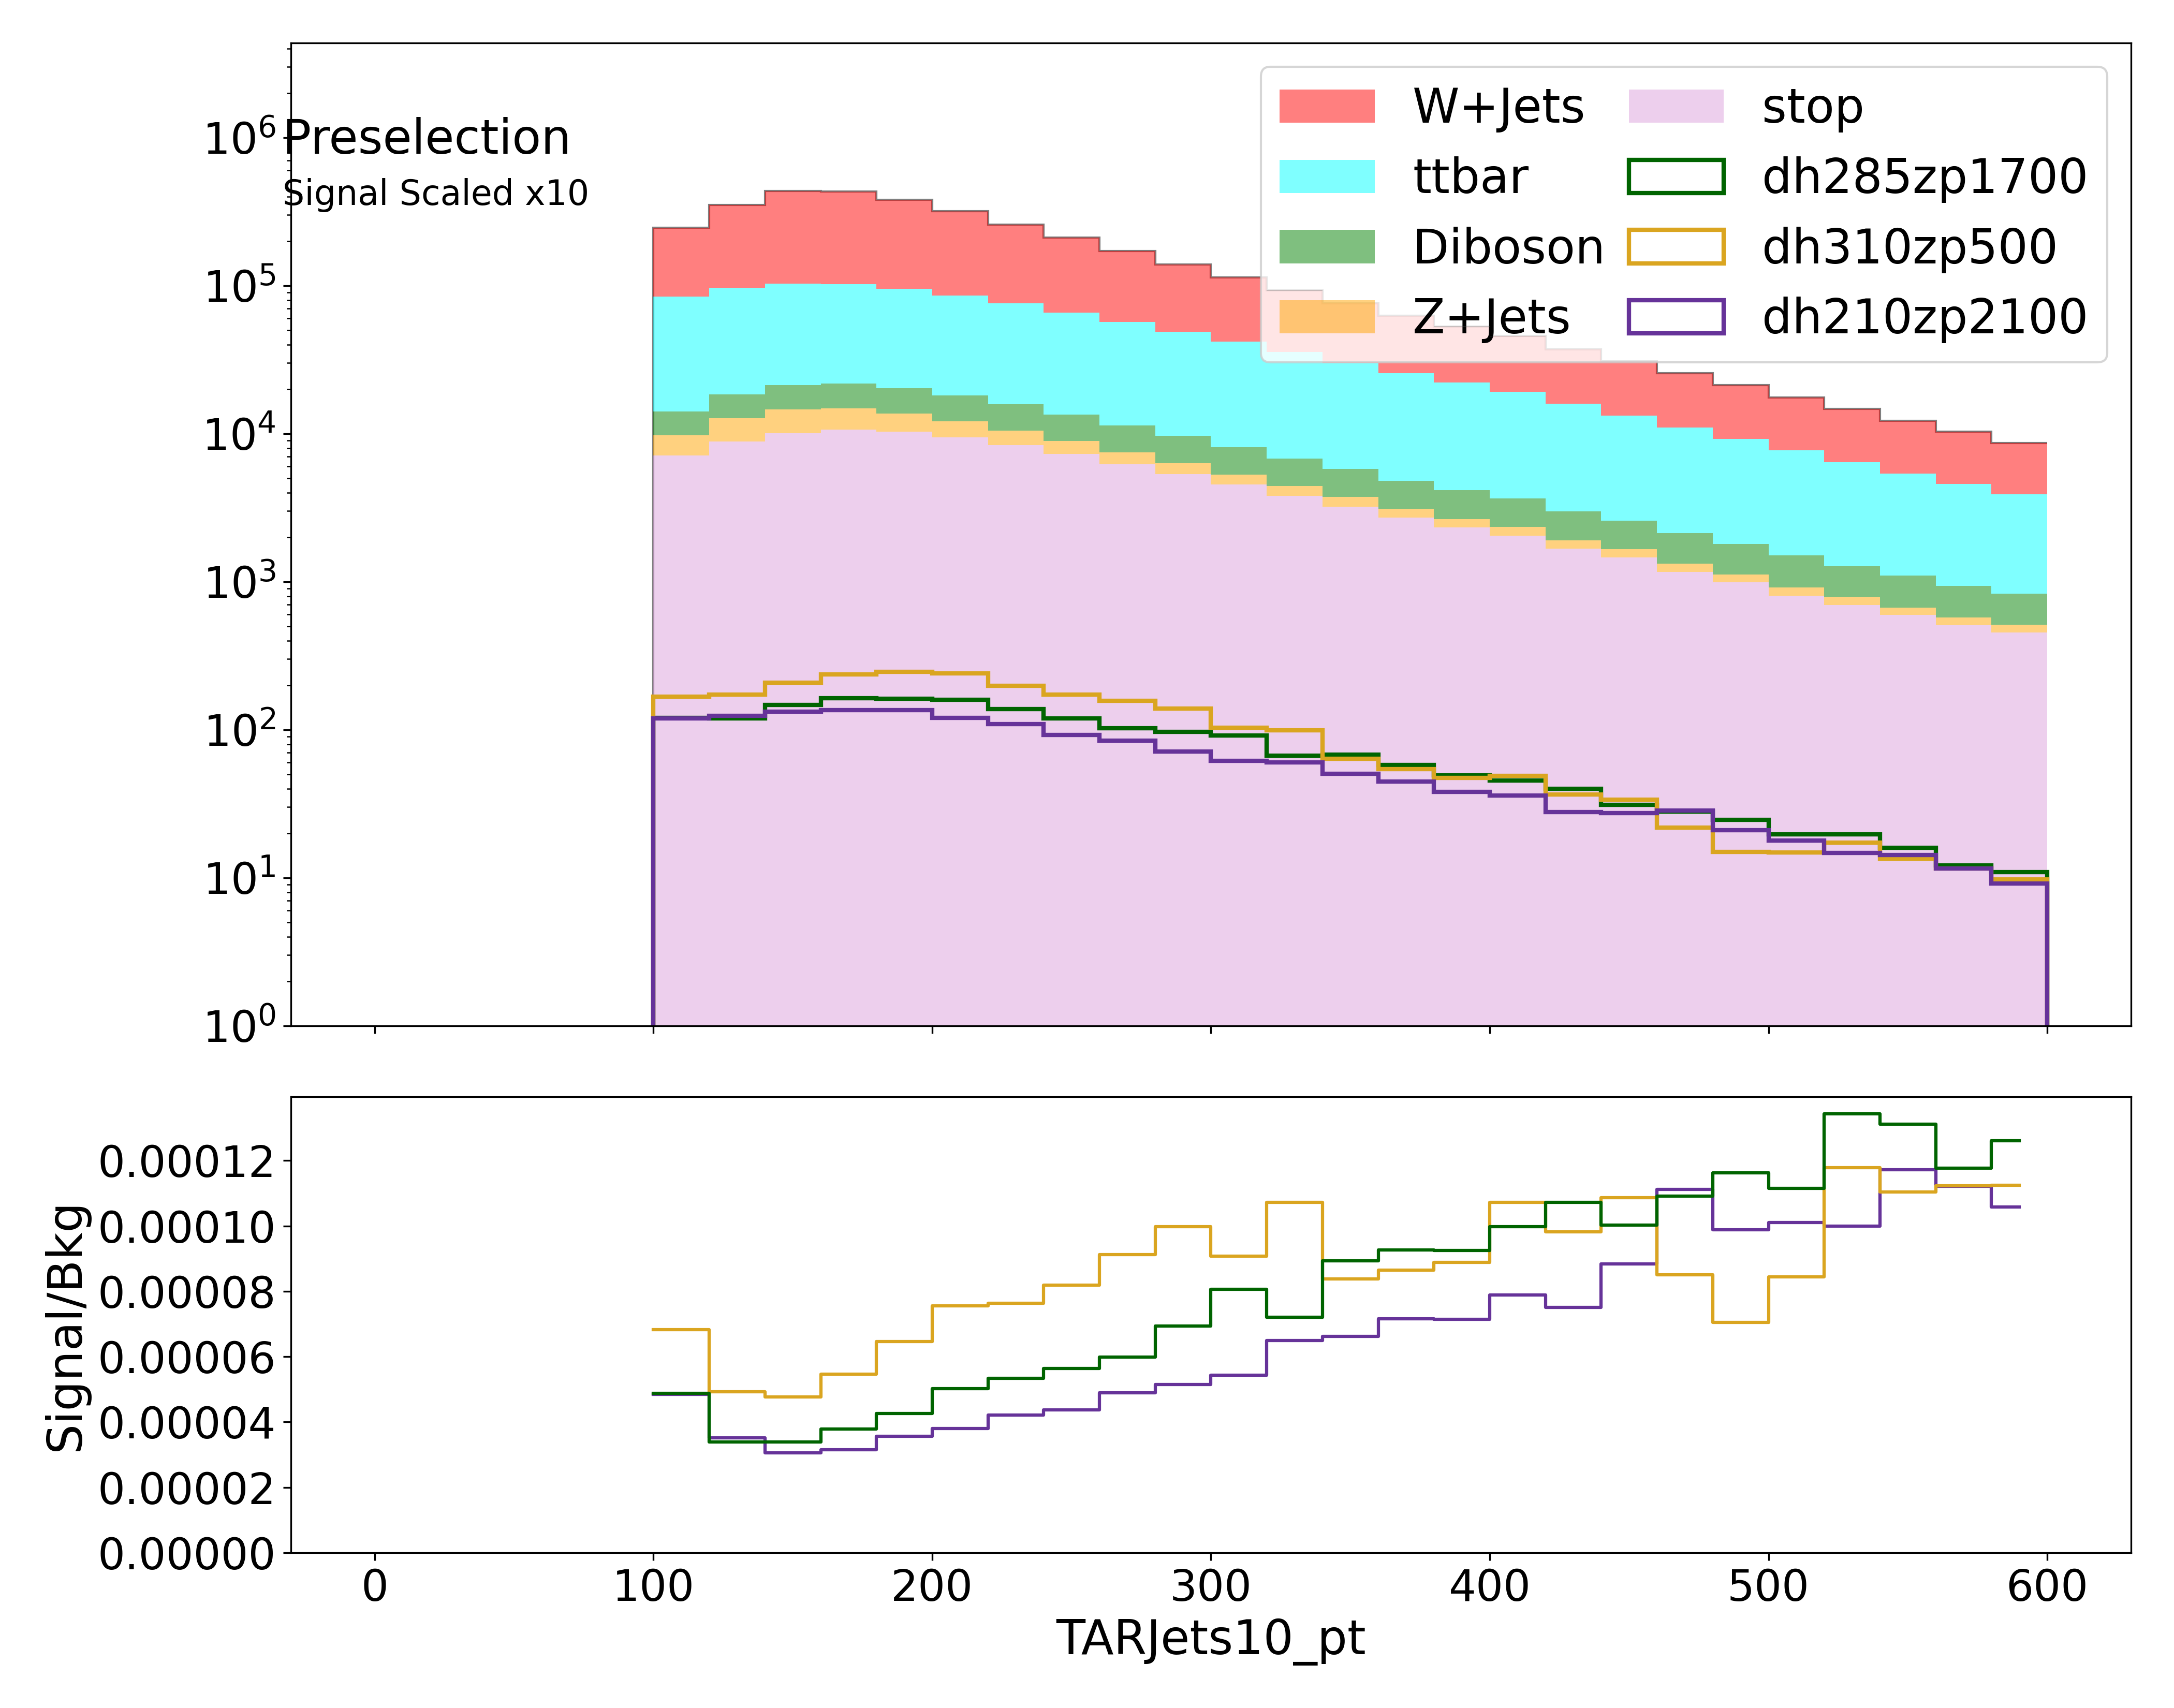
\includegraphics[width = 0.98\textwidth]{Figures/appendix/Preselection/TARJets10_pt.png}
      \caption{$\pT(\text{TAR})$}
      \end{subfigure}
      \caption{Preselection level distribuitions. Grey bands represent MC statistical uncertainty on each bin.}
      \label{fig:Presel2}
    \end{figure}

    \begin{figure}[htbp]
      \centering
      \begin{subfigure}{0.49\textwidth}
      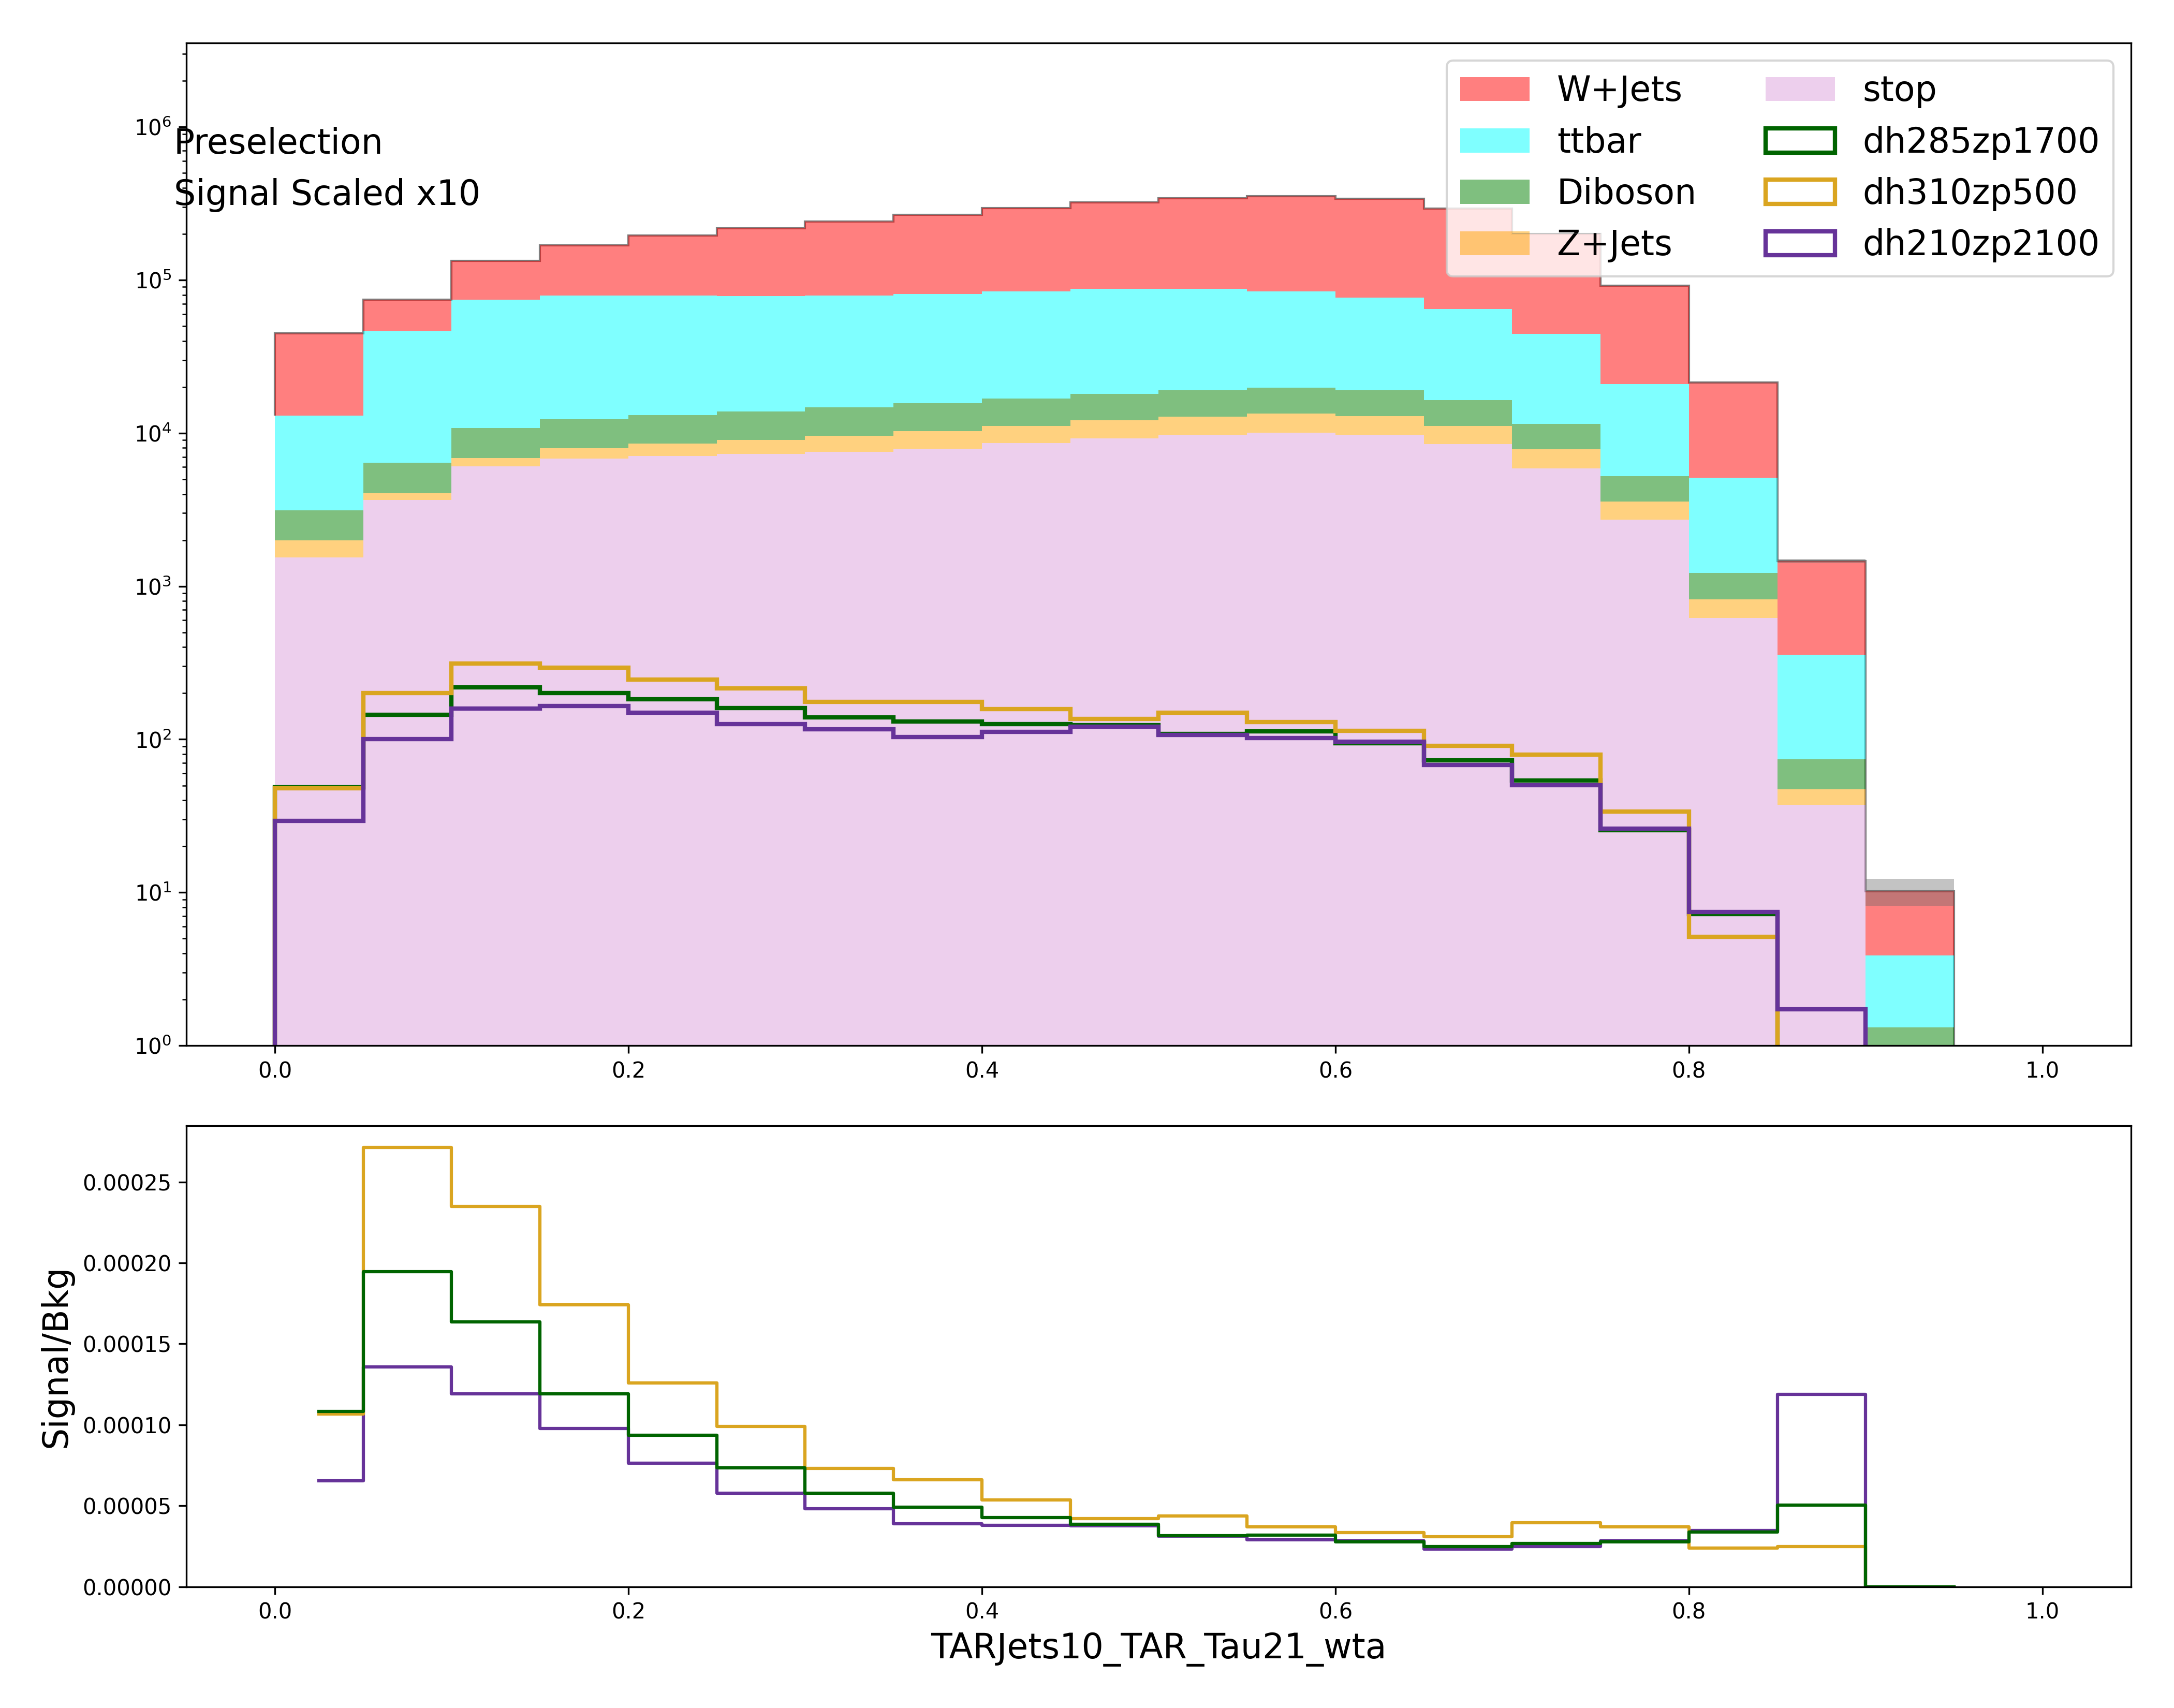
\includegraphics[width = 0.98\textwidth]{Figures/appendix/Preselection/TARJets10_TAR_Tau21_wta.png}
      \caption{$\tau_{21}(\text{TAR})$}
      \end{subfigure}
      \begin{subfigure}{0.49\textwidth}
      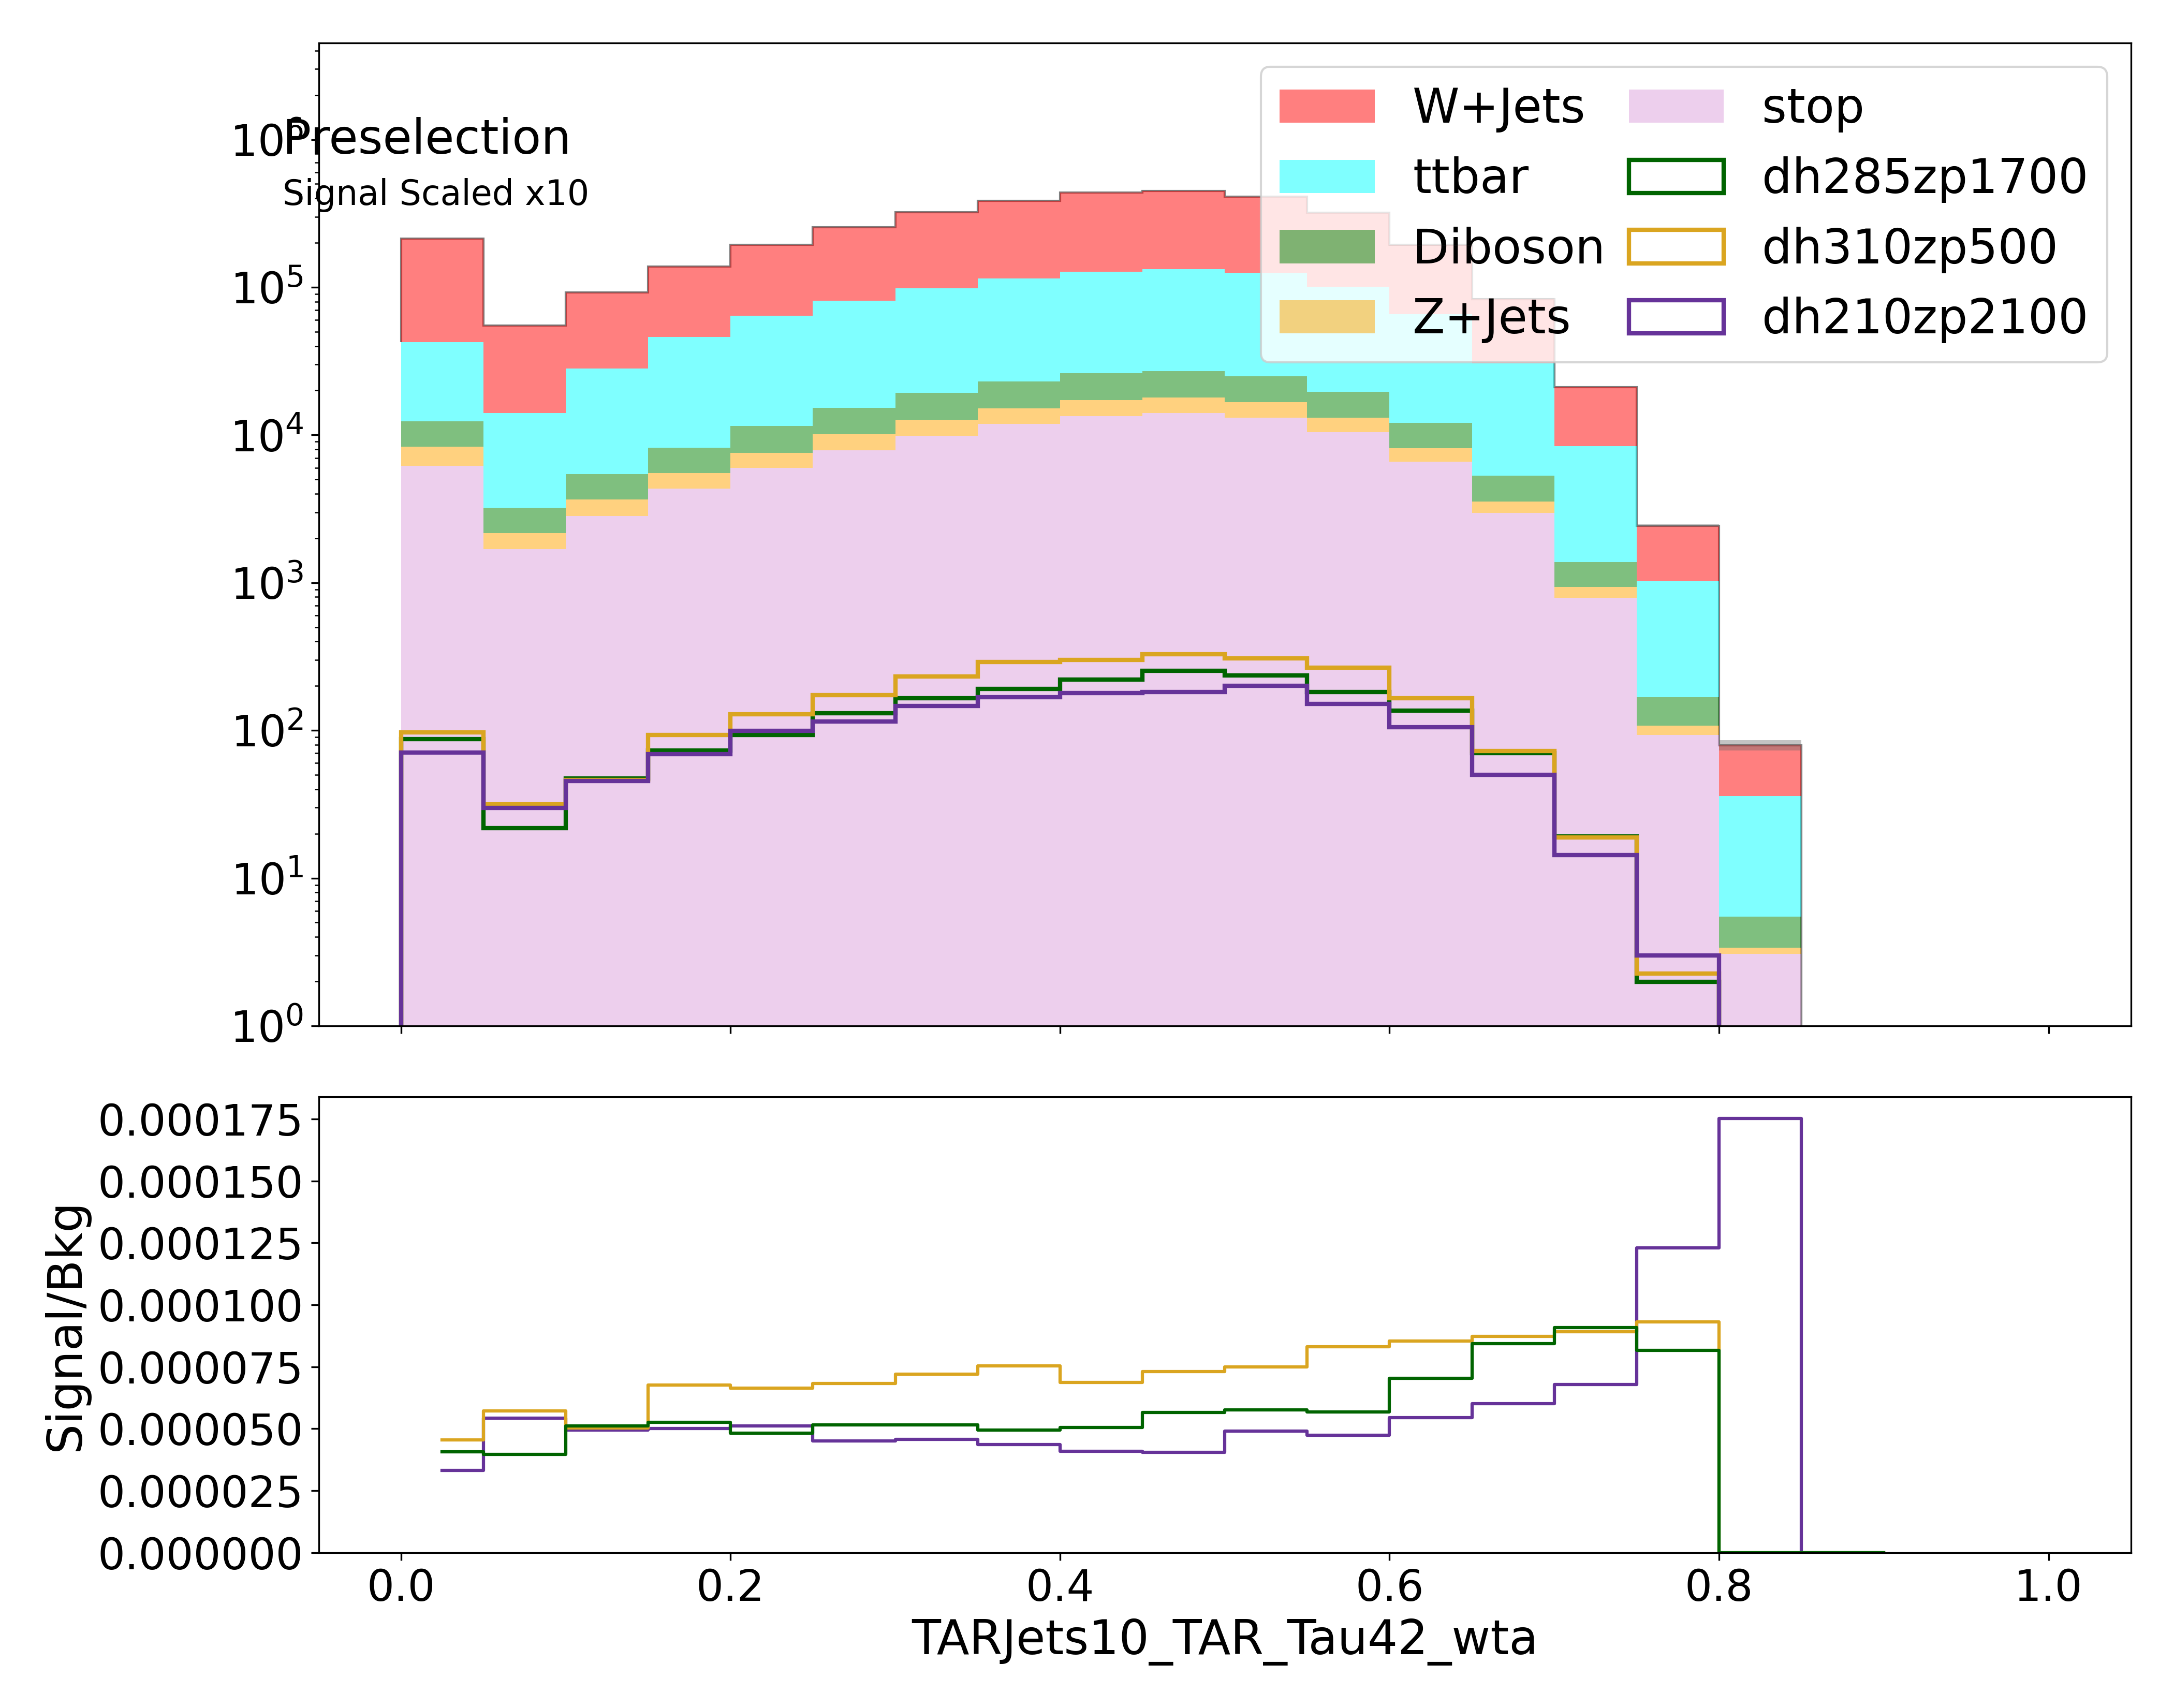
\includegraphics[width = 0.98\textwidth]{Figures/appendix/Preselection/TARJets10_TAR_Tau42_wta.png}
      \caption{$\tau_{42}(\text{TAR})$}
      \end{subfigure}
         \begin{subfigure}{0.49\textwidth}
         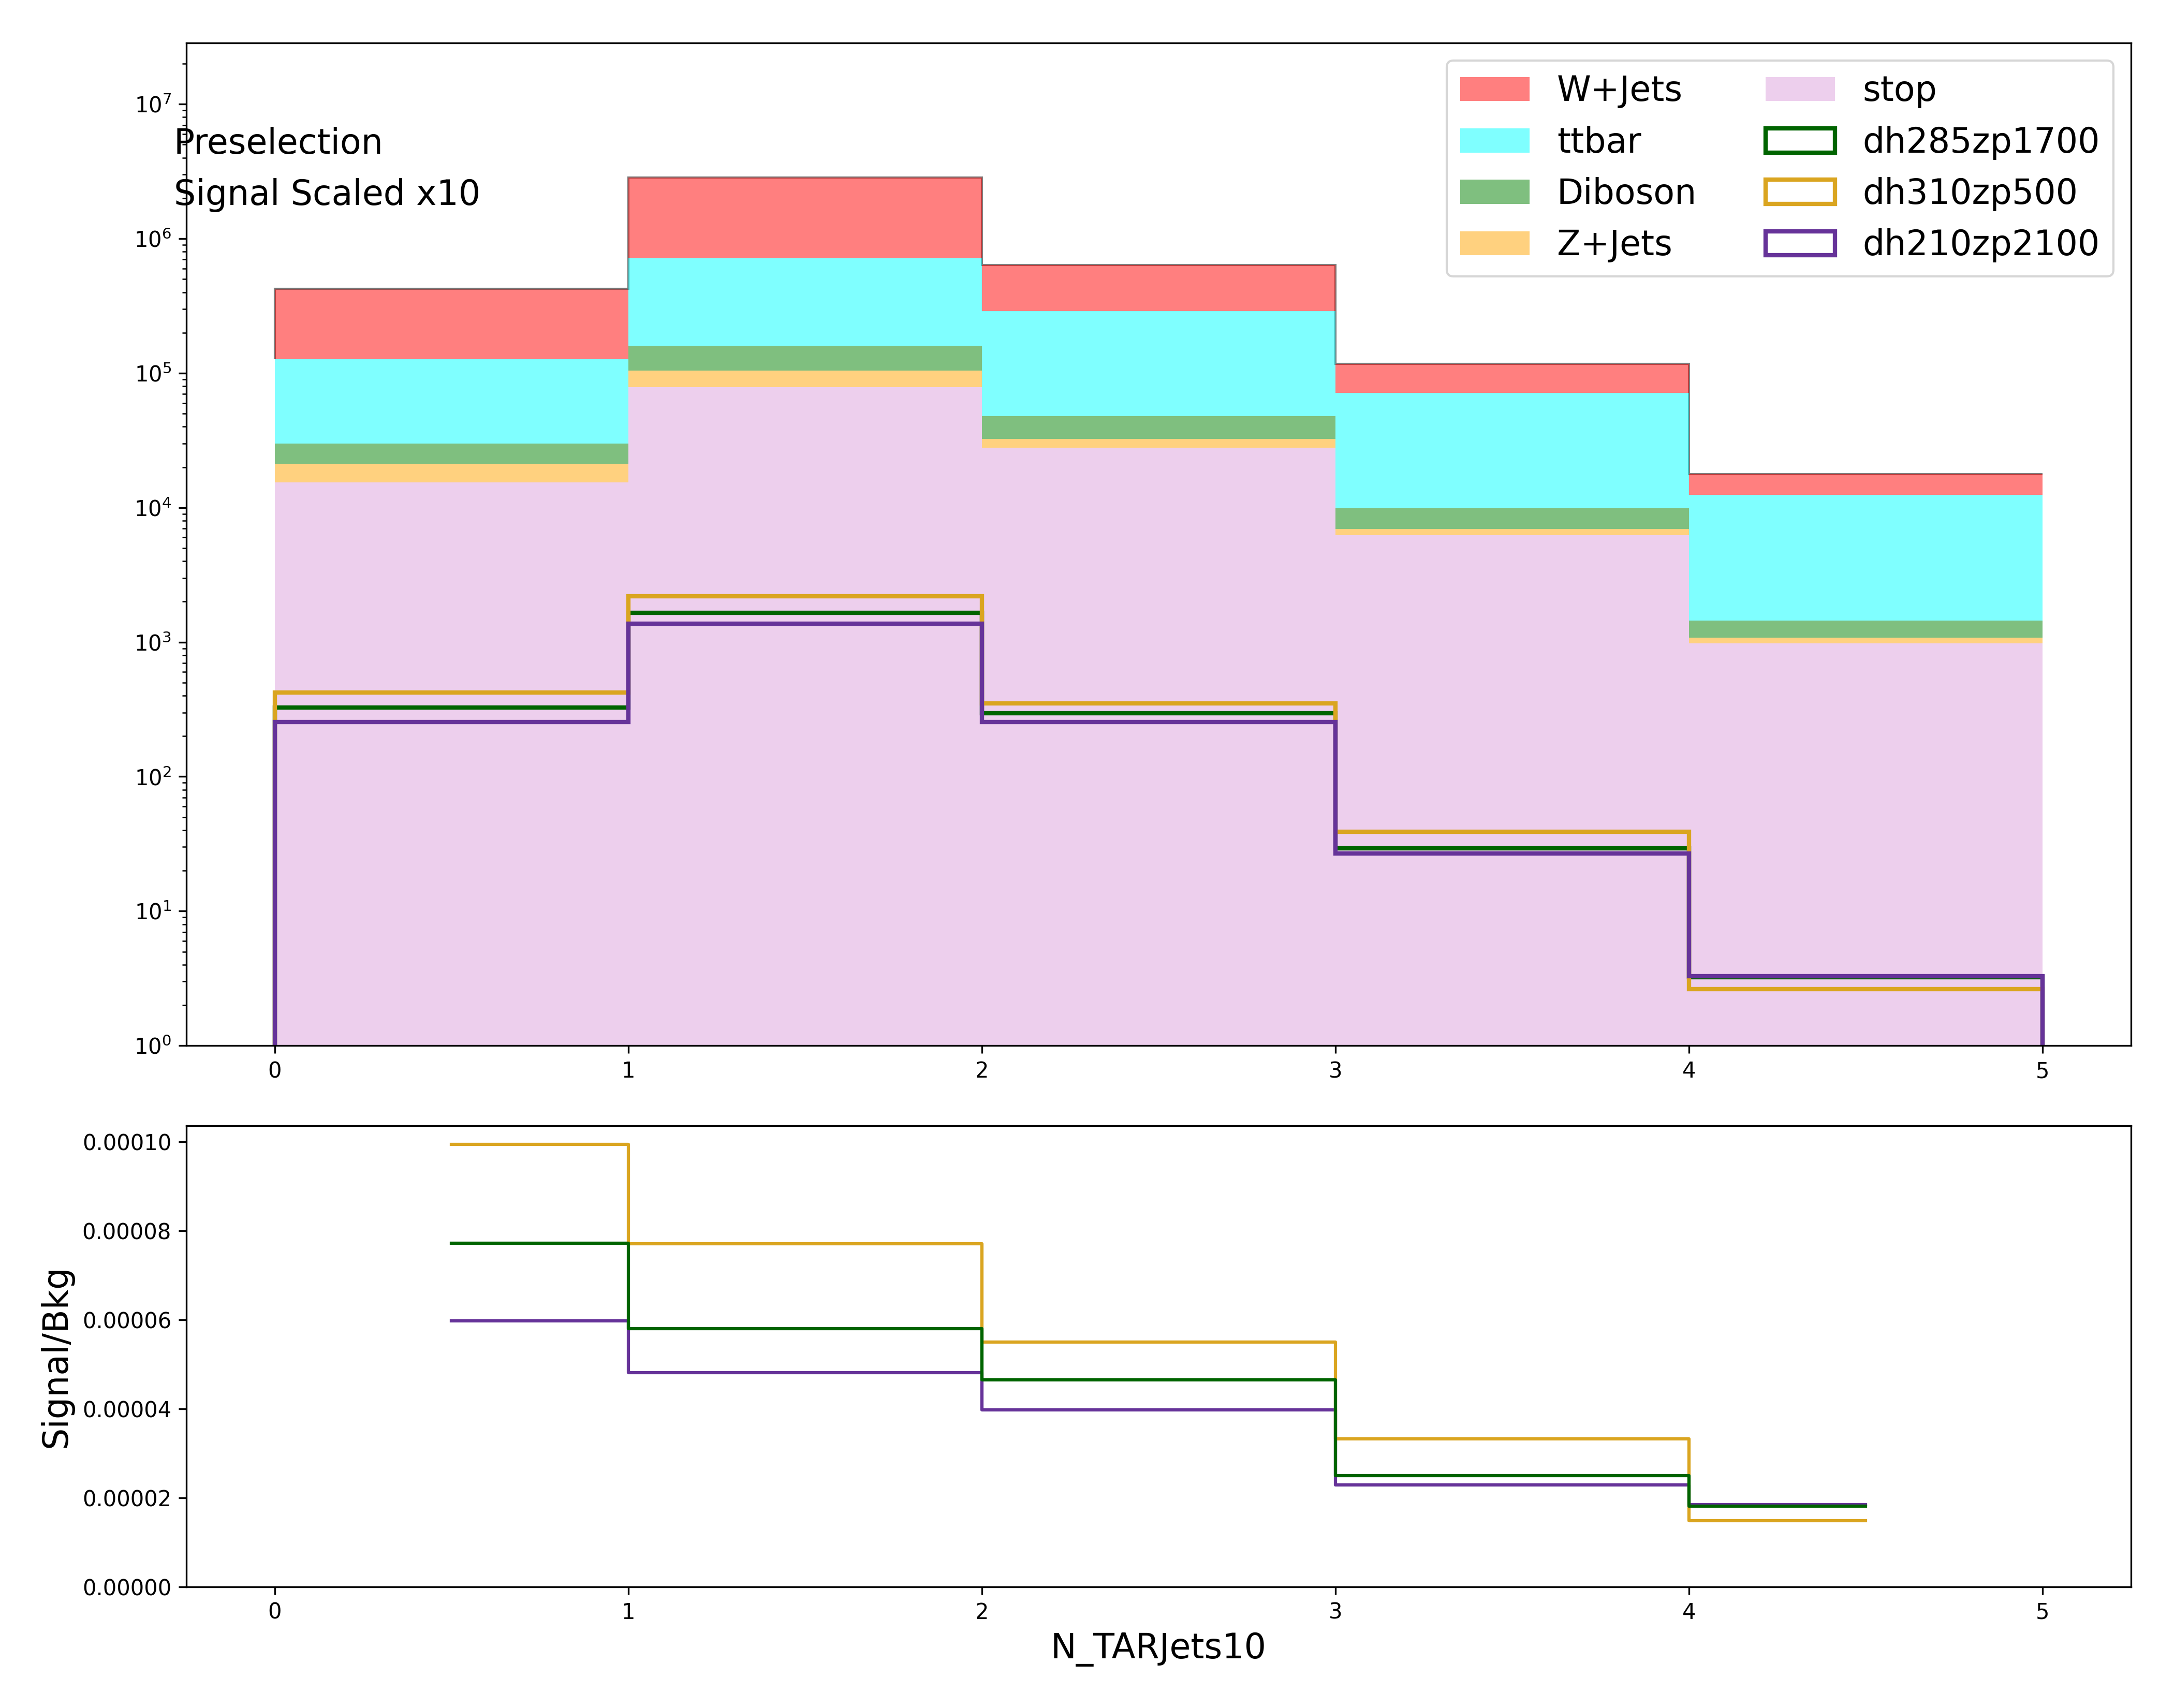
\includegraphics[width = 0.98\textwidth]{Figures/appendix/Preselection/N_TARJets10.png}
         \caption{\NTAR}
         \end{subfigure}
         \begin{subfigure}{0.49\textwidth}
         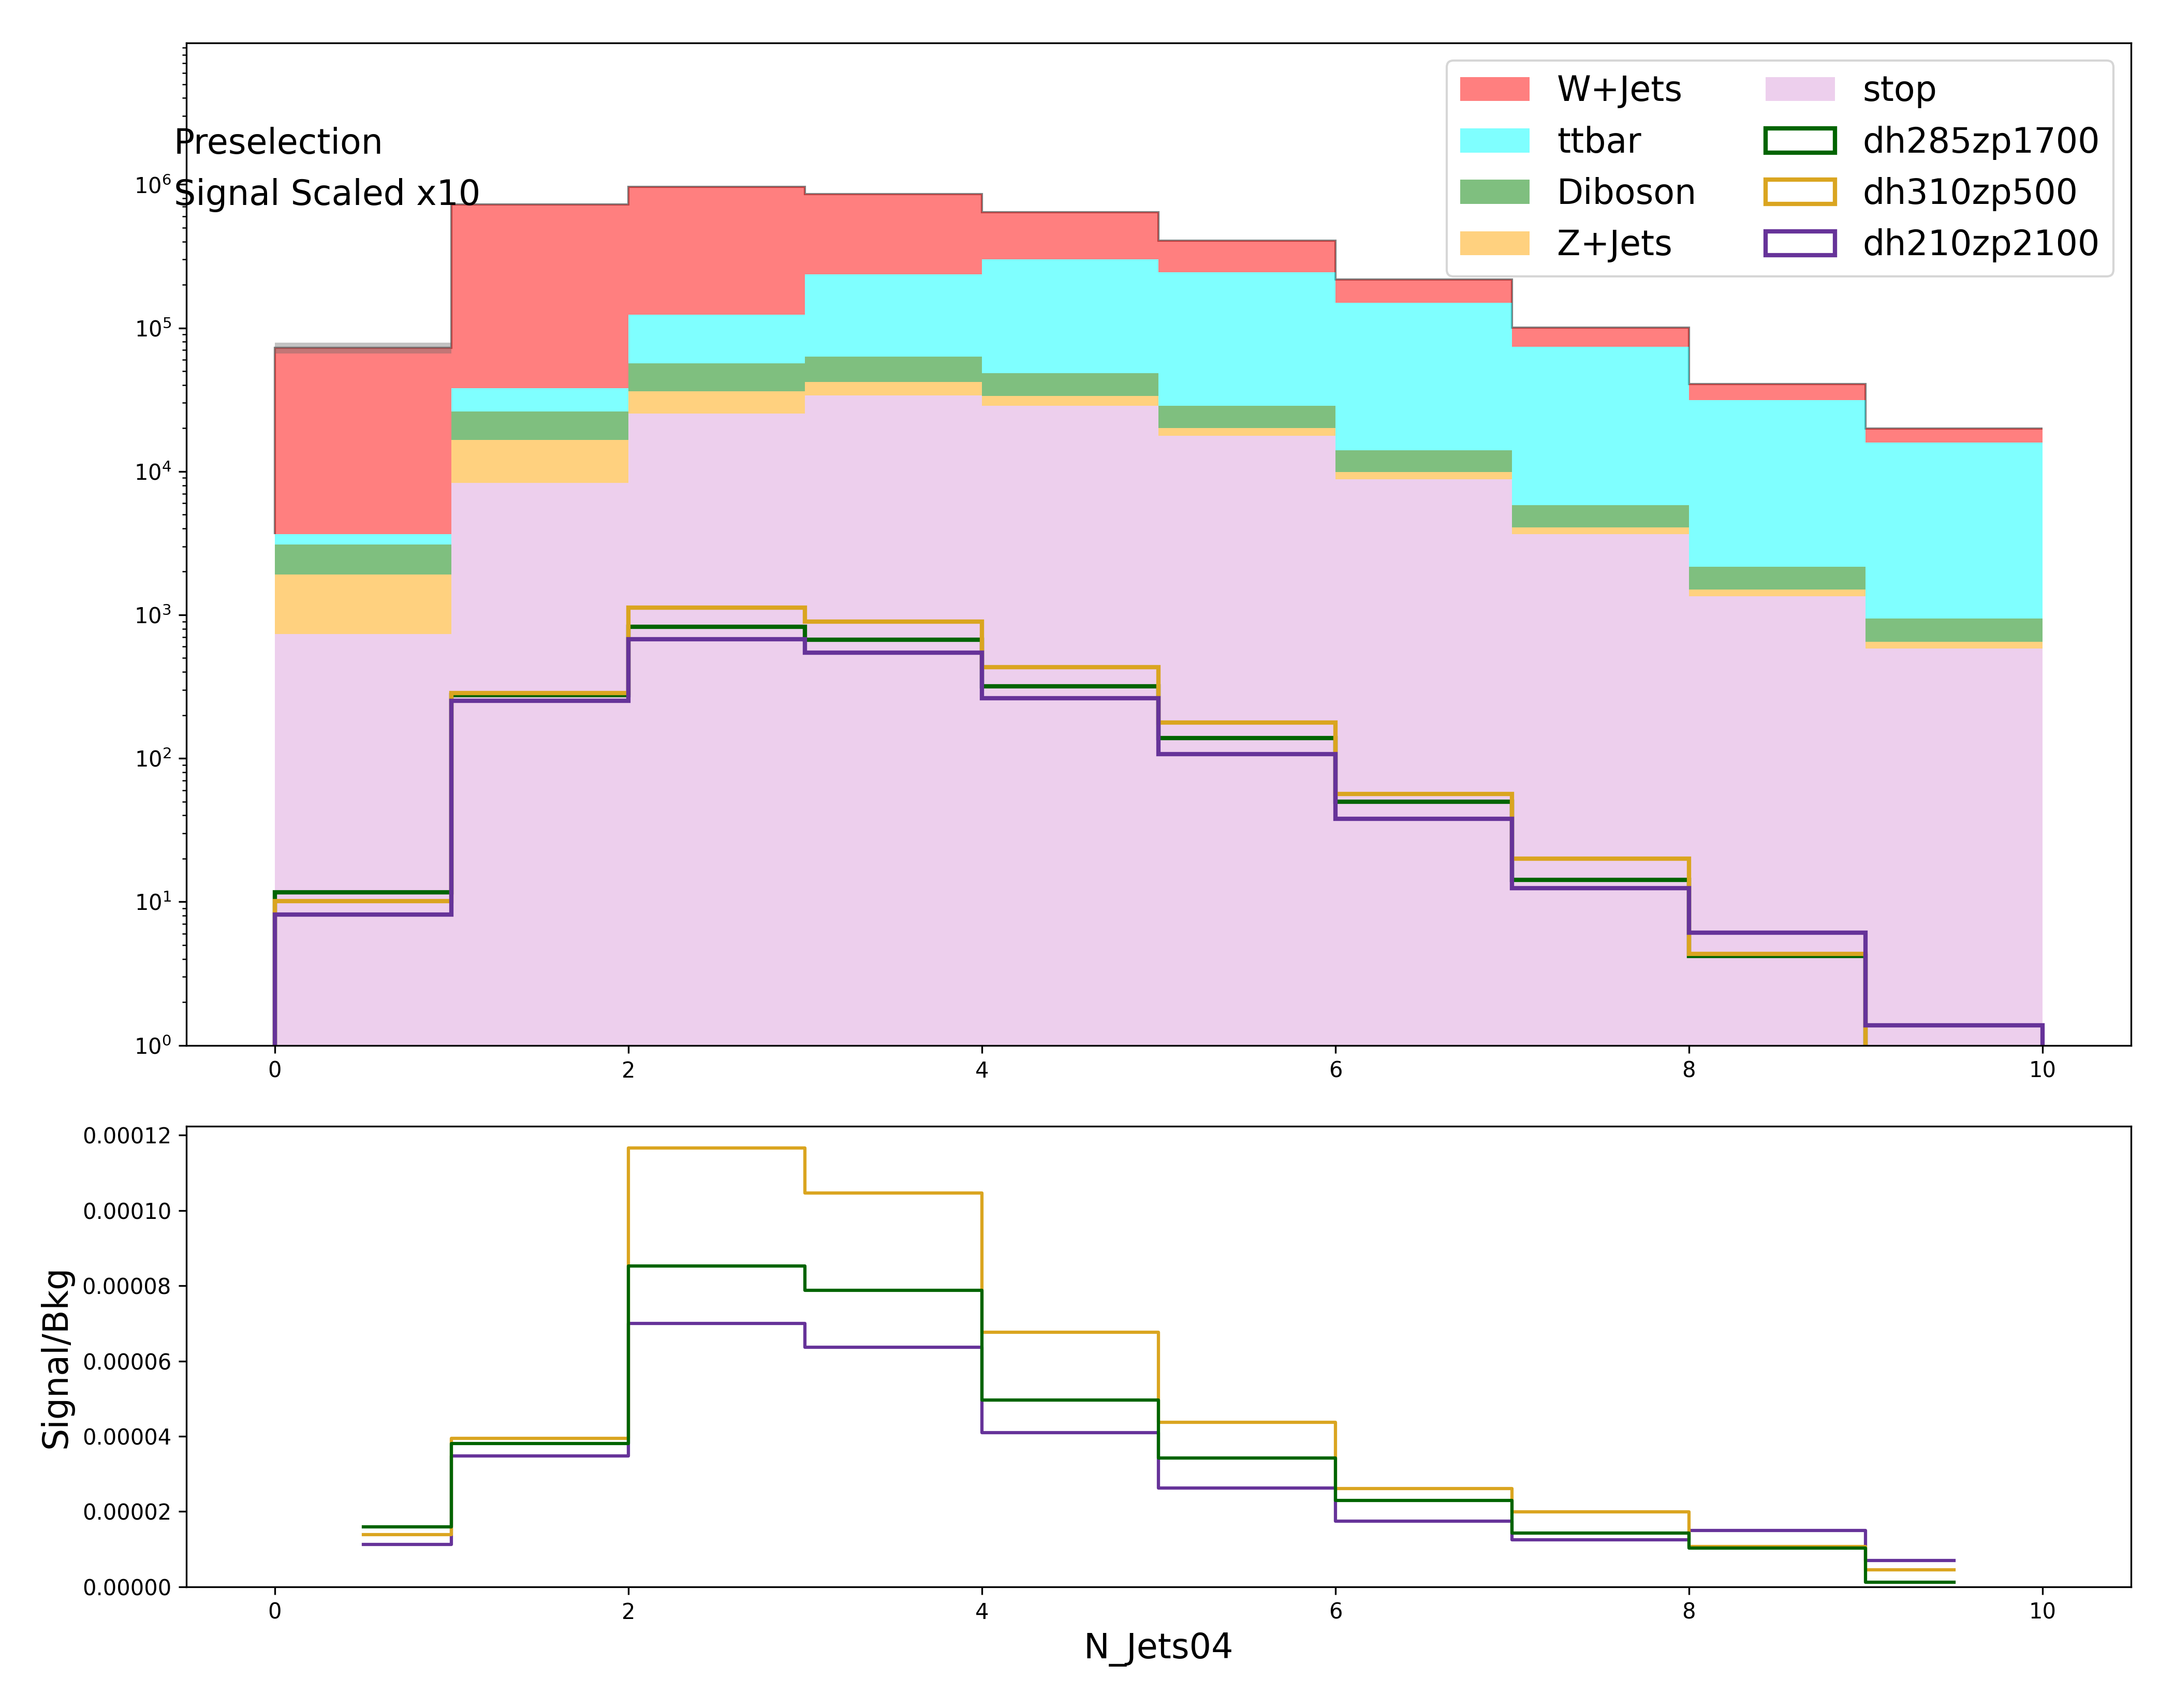
\includegraphics[width = 0.98\textwidth]{Figures/appendix/Preselection/N_Jets04.png}
         \caption{\Njets}
         \end{subfigure}
         \begin{subfigure}{0.49\textwidth}
         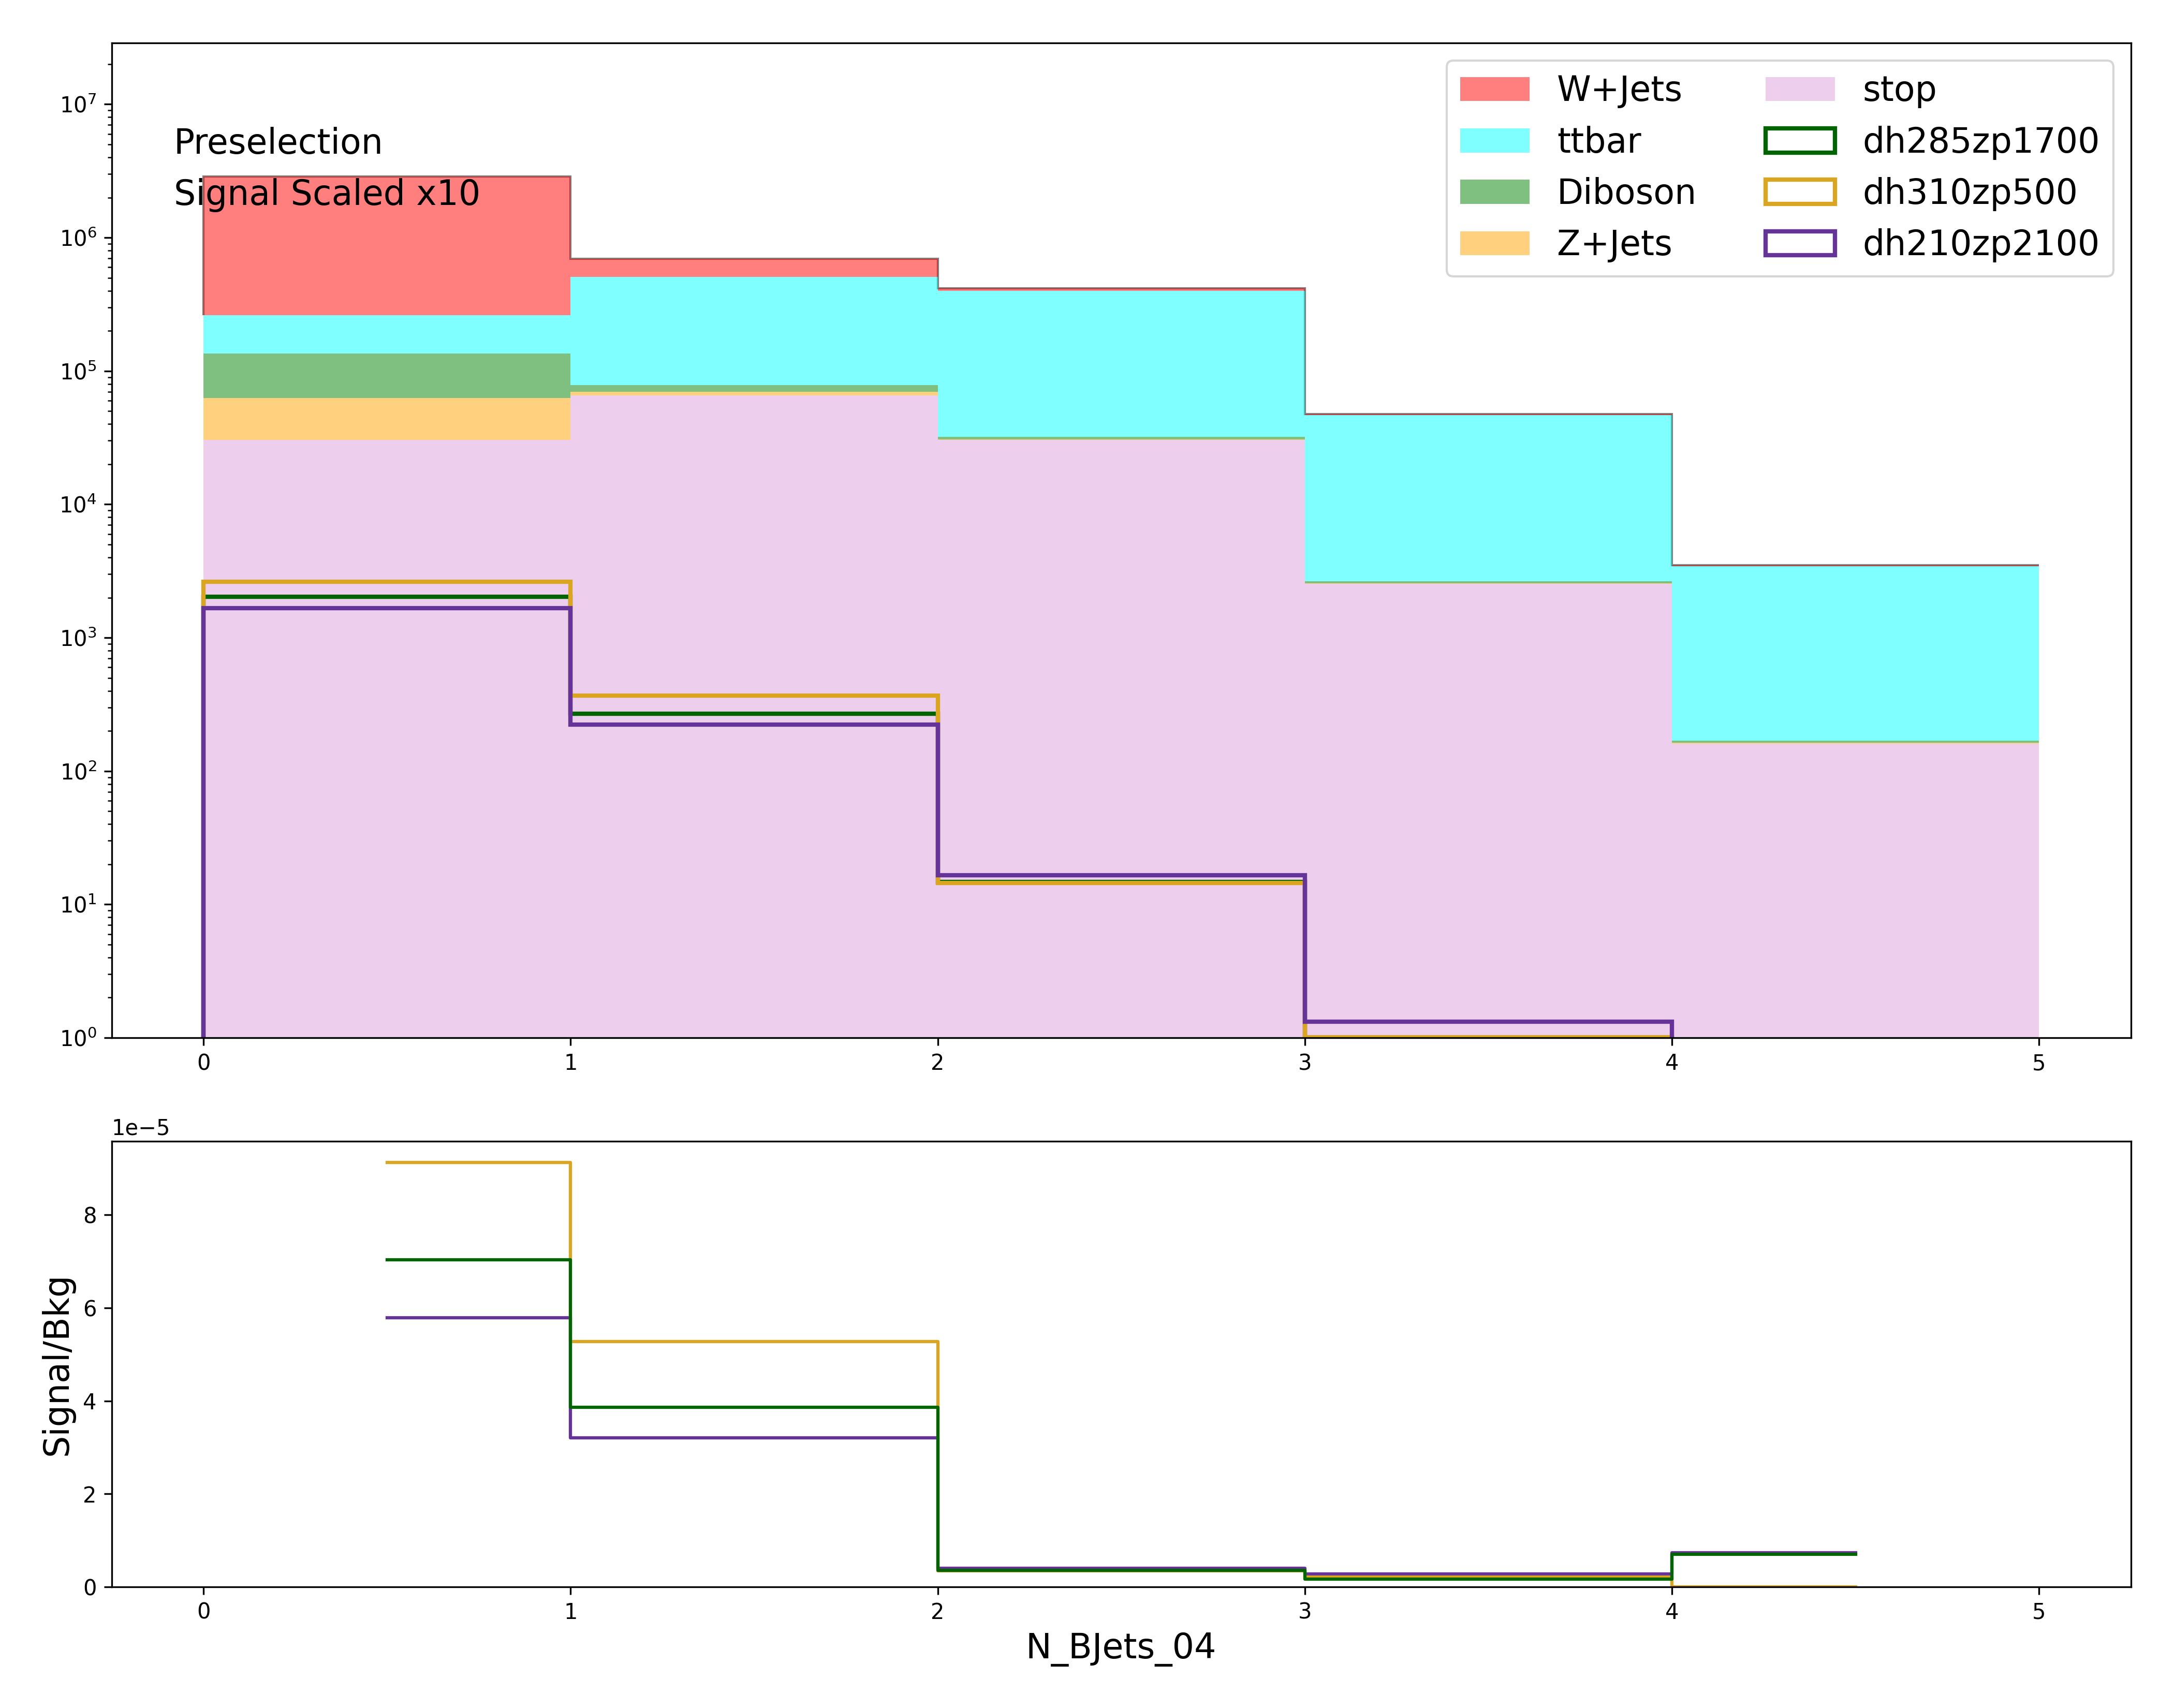
\includegraphics[width = 0.98\textwidth]{Figures/appendix/Preselection/N_BJets_04.png}
         \caption{\ensuremath{N (\text{b-Jets})}\xspace}
         \end{subfigure}
         \begin{subfigure}{0.49\textwidth}
         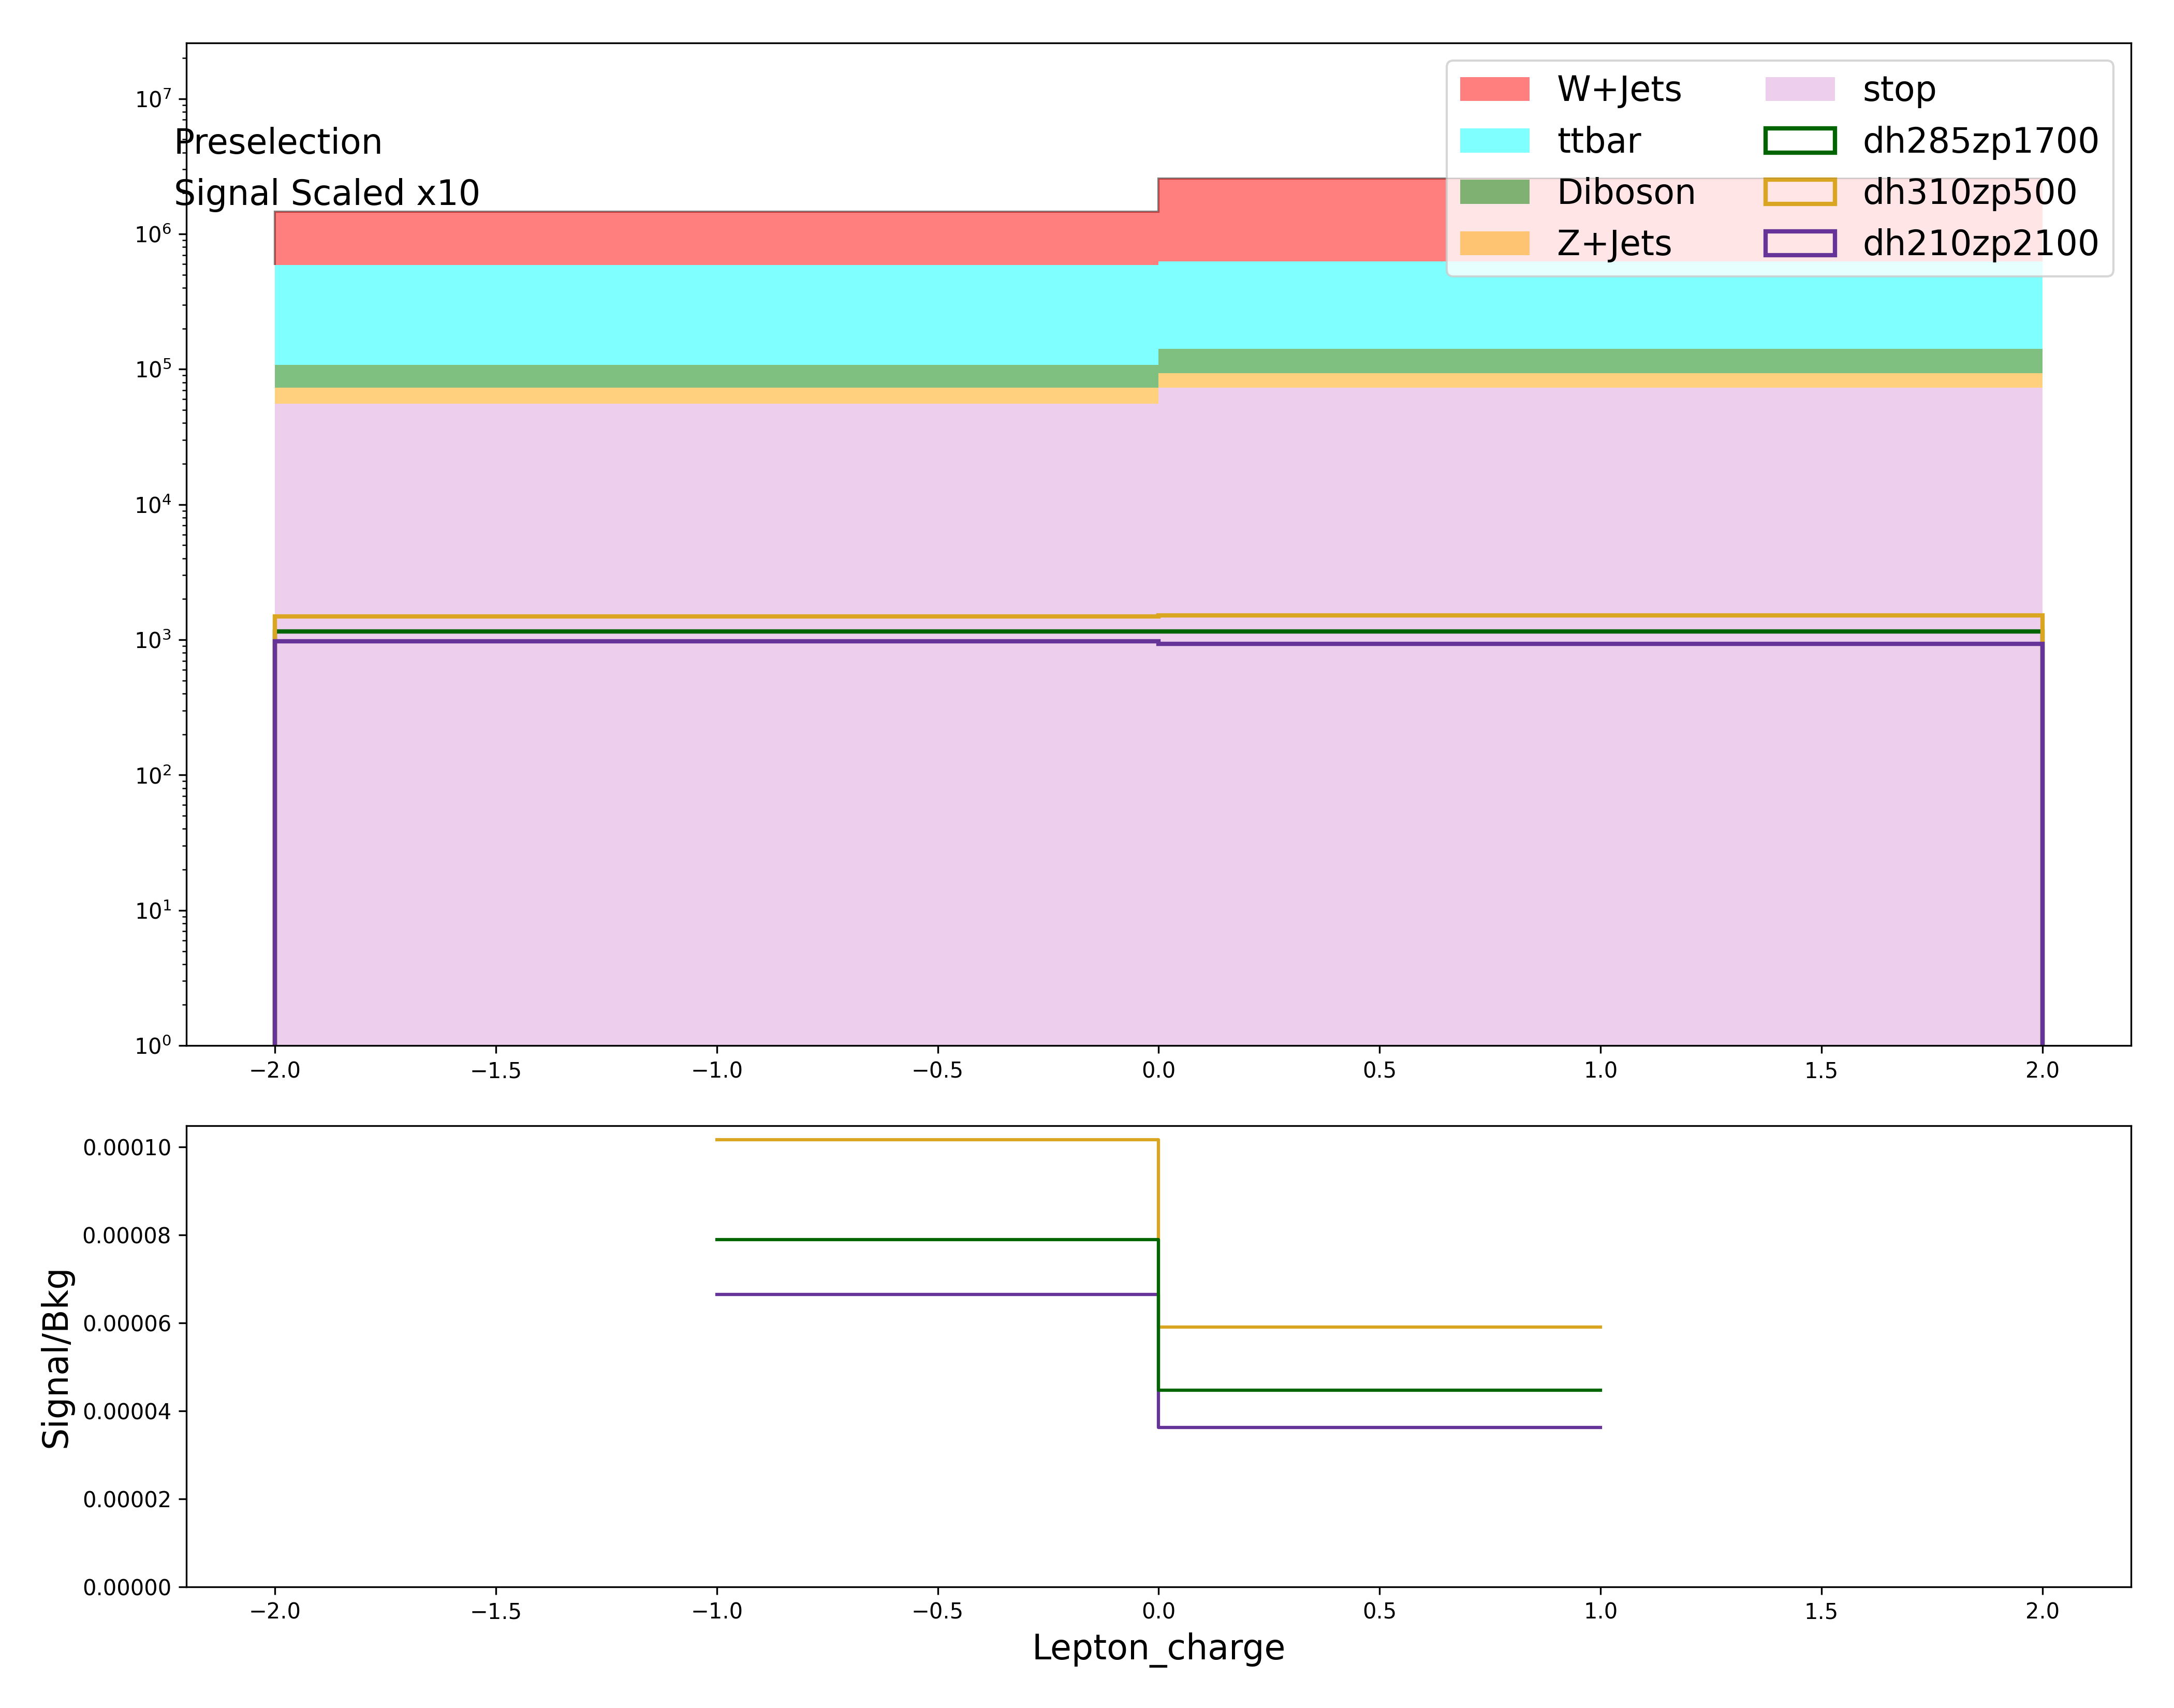
\includegraphics[width = 0.98\textwidth]{Figures/appendix/Preselection/Lepton_charge.png}
         \caption{$\text{charge}(\ell)$}
         \end{subfigure}

         \caption{Preselection level distribuitions. Grey bands represent MC statistical uncertainty on each bin.}
         \label{fig:Presel3}
      \end{figure}
\FloatBarrier

\section{Data-MC Comparisons in Control Regions}
\label{section:datamc}
The following section contains plots comparing data and MC distributions in the control regions. MC events are normalized to the luminosity measured in data as described in Chapter \ref{chapter:ana_prep} subsection \ref{subsubsection:mc_scaling}. The uncertainties shown on both data and MC events in these plots are purely statistical and do not include uncertainties on the modelling of background events, which impact the cross-section of the different categories of background events. Some statistically significant differences between data and MC are therefore not unexpected.
\subsection{\ttbar Control Regions}

\begin{figure}[htbp]
  \centering

     \begin{subfigure}{0.49\textwidth}
     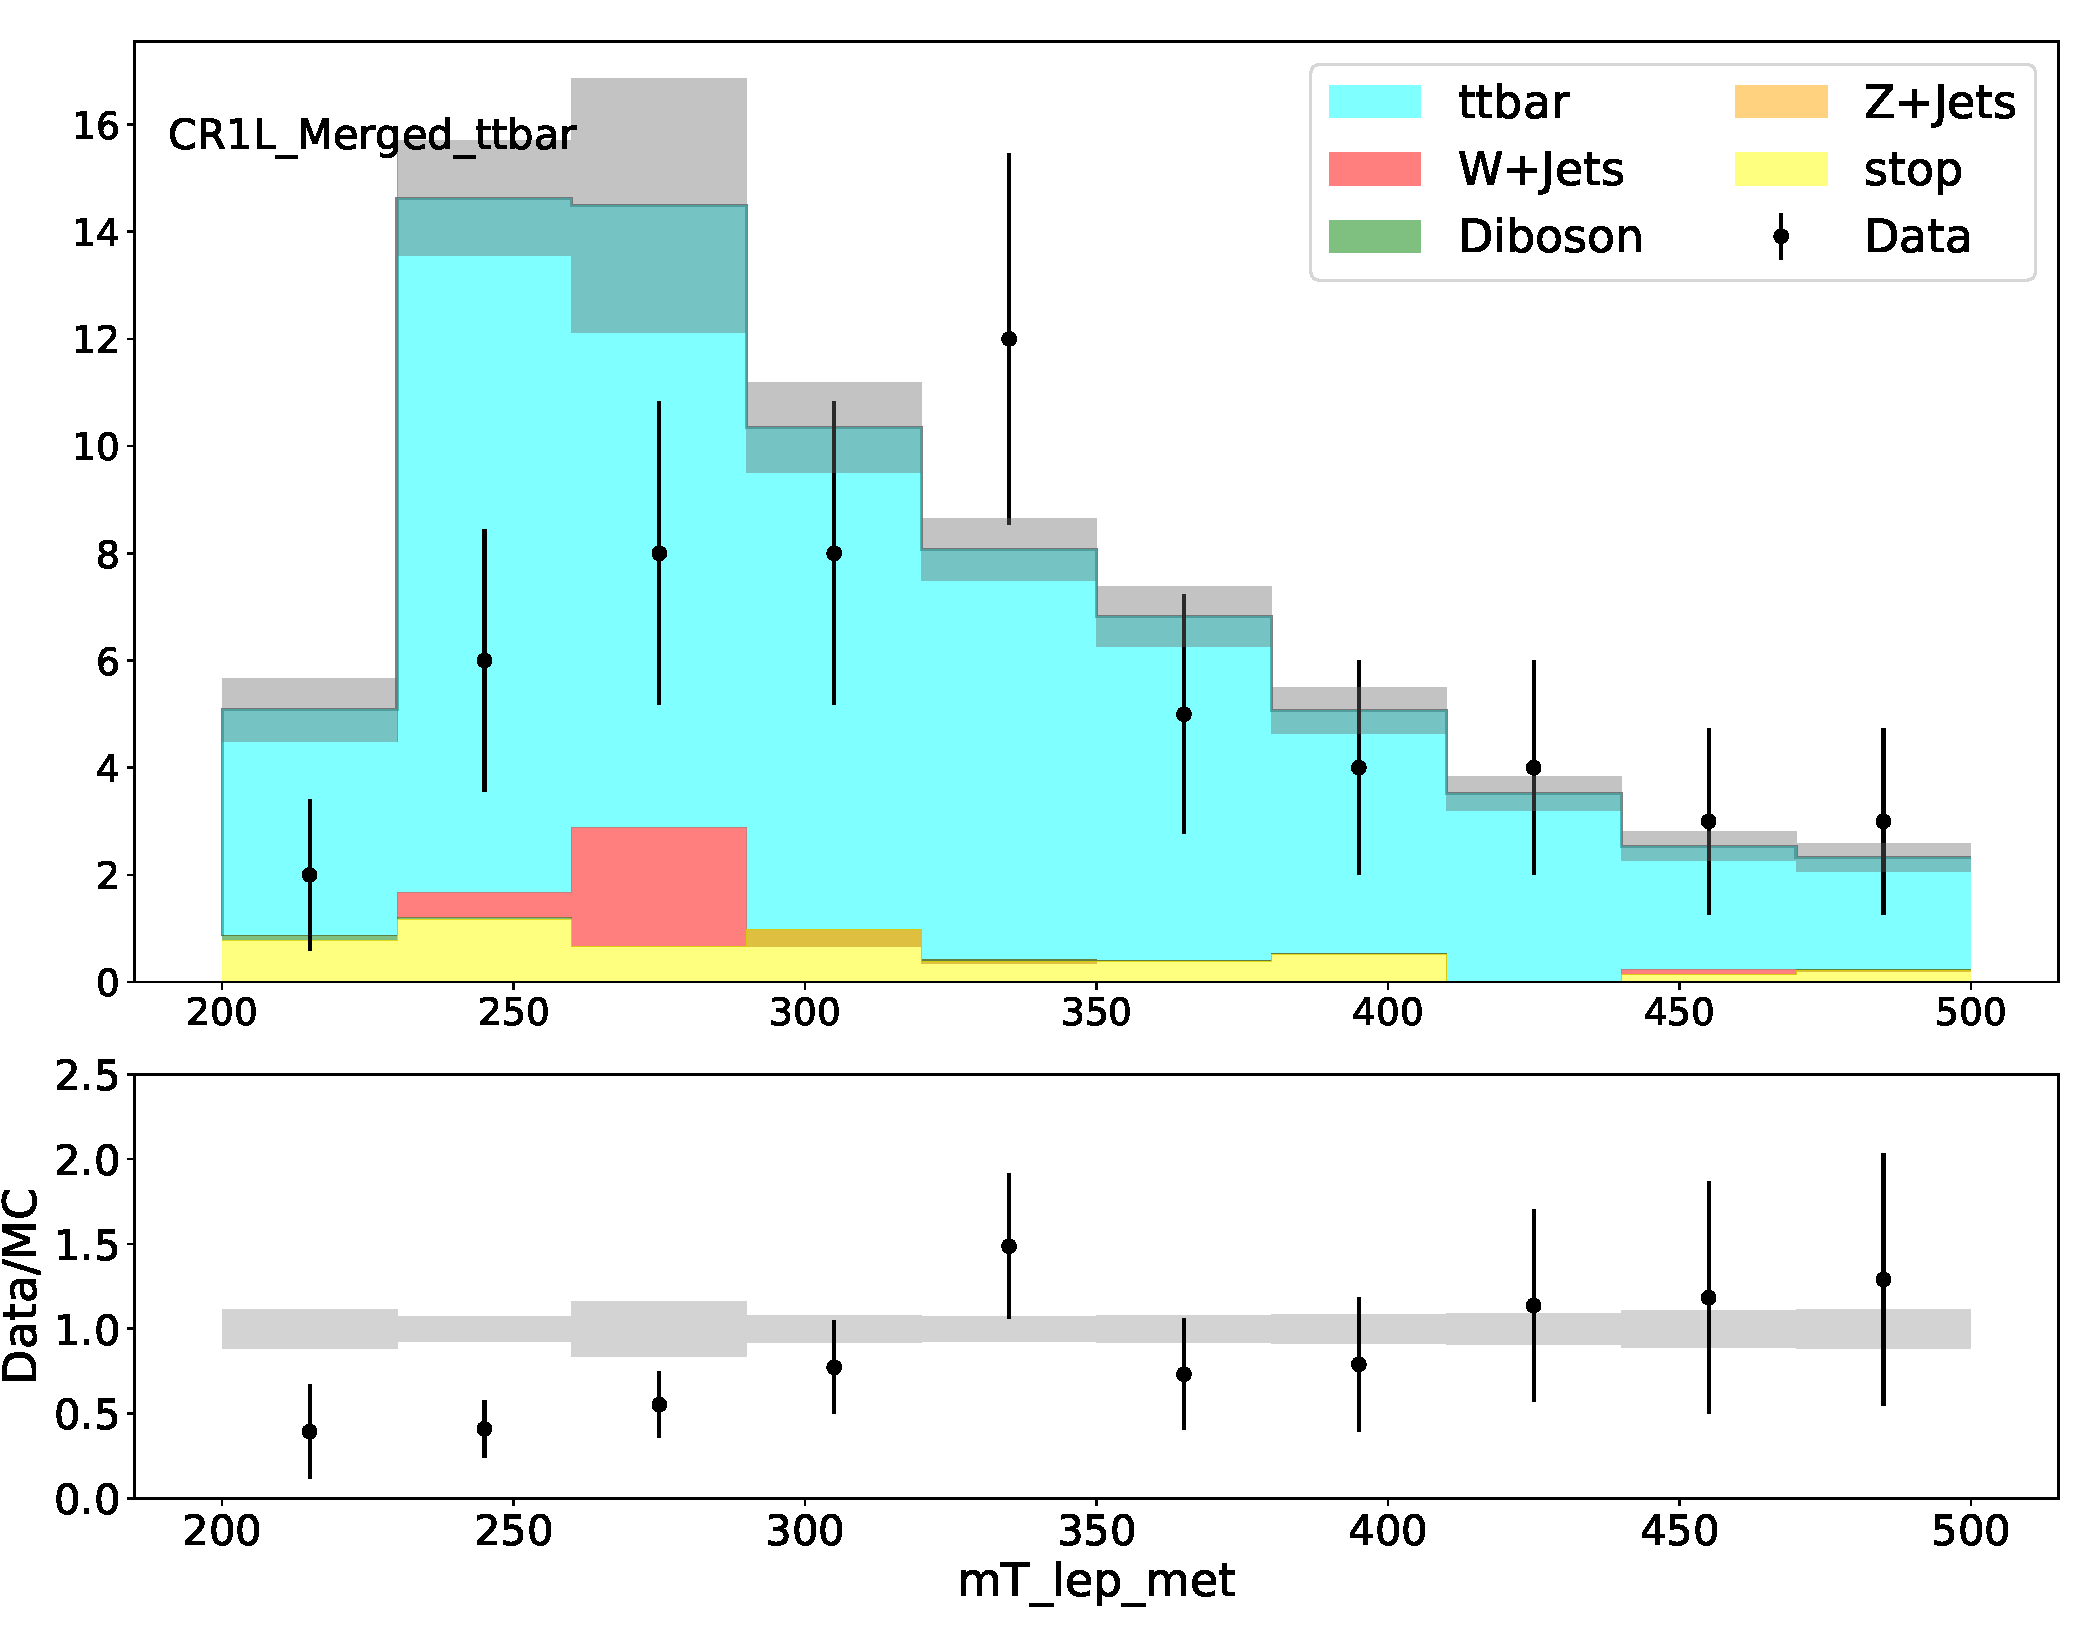
\includegraphics[width = 0.98\textwidth]{Figures/4/datamc/CR1L_Merged_ttbar/mT_lep_met.pdf}
     \caption{\mtlepmet}
     \end{subfigure}
     \begin{subfigure}{0.49\textwidth}
     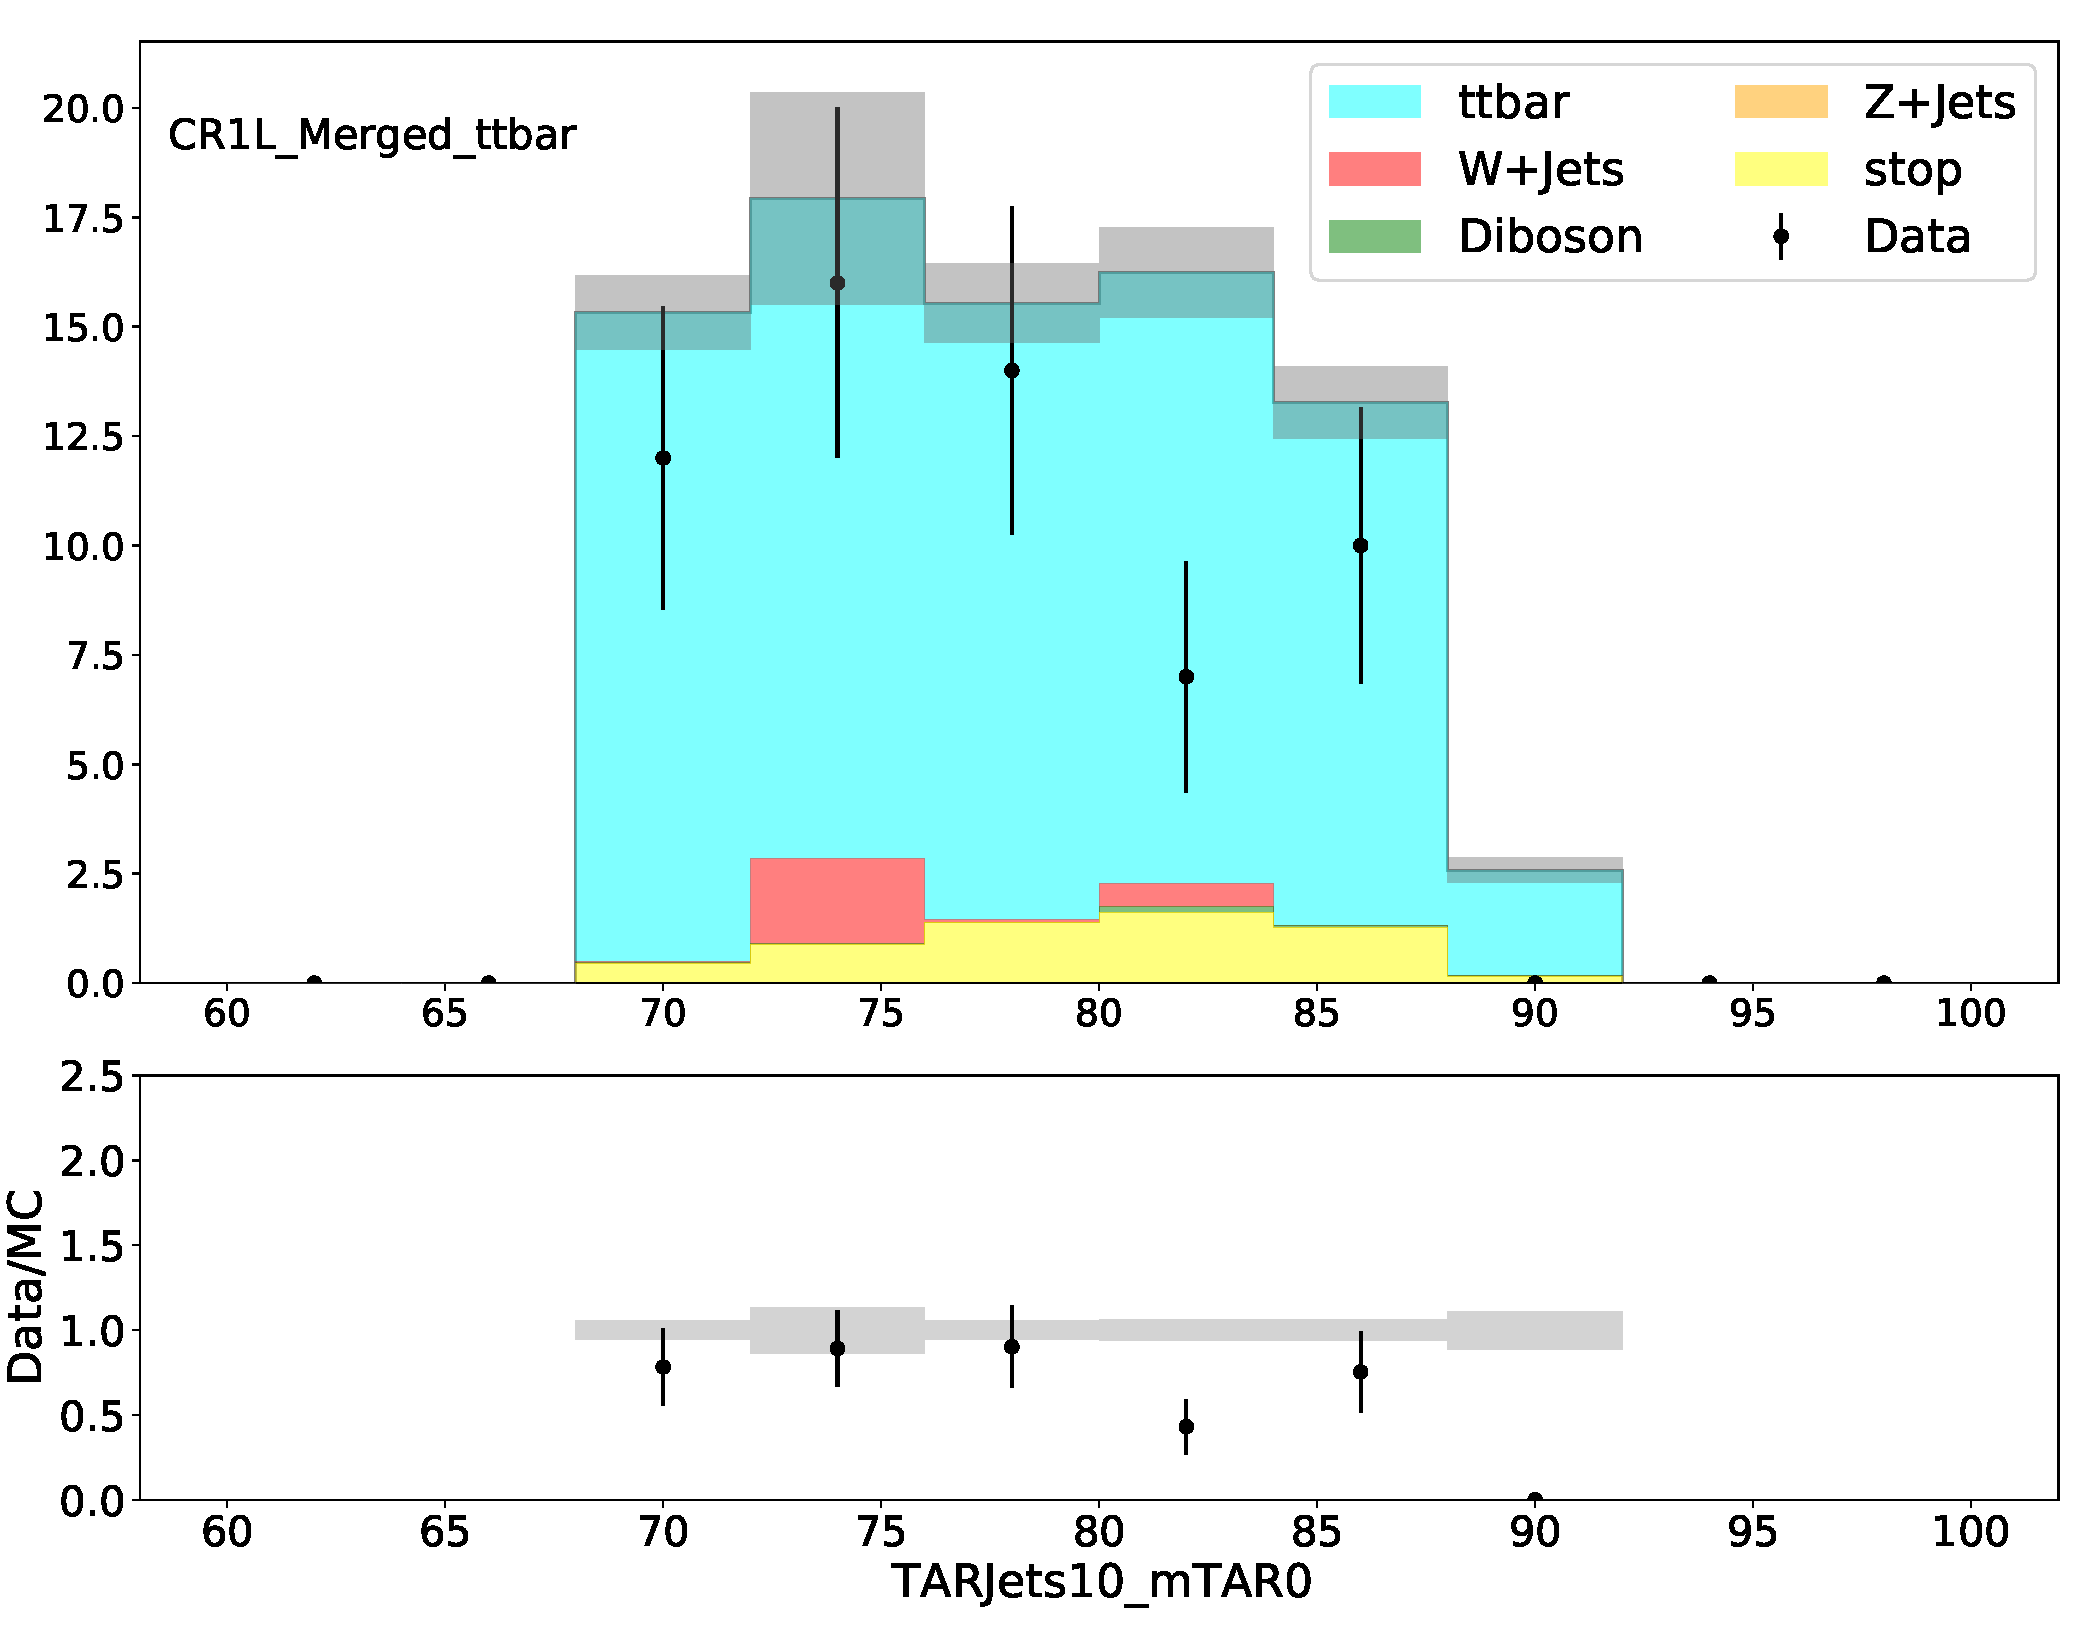
\includegraphics[width = 0.98\textwidth]{Figures/4/datamc/CR1L_Merged_ttbar/TARJets10_mTAR0.pdf}
     \caption{\mTAR}
     \end{subfigure}
     \begin{subfigure}{0.49\textwidth}
     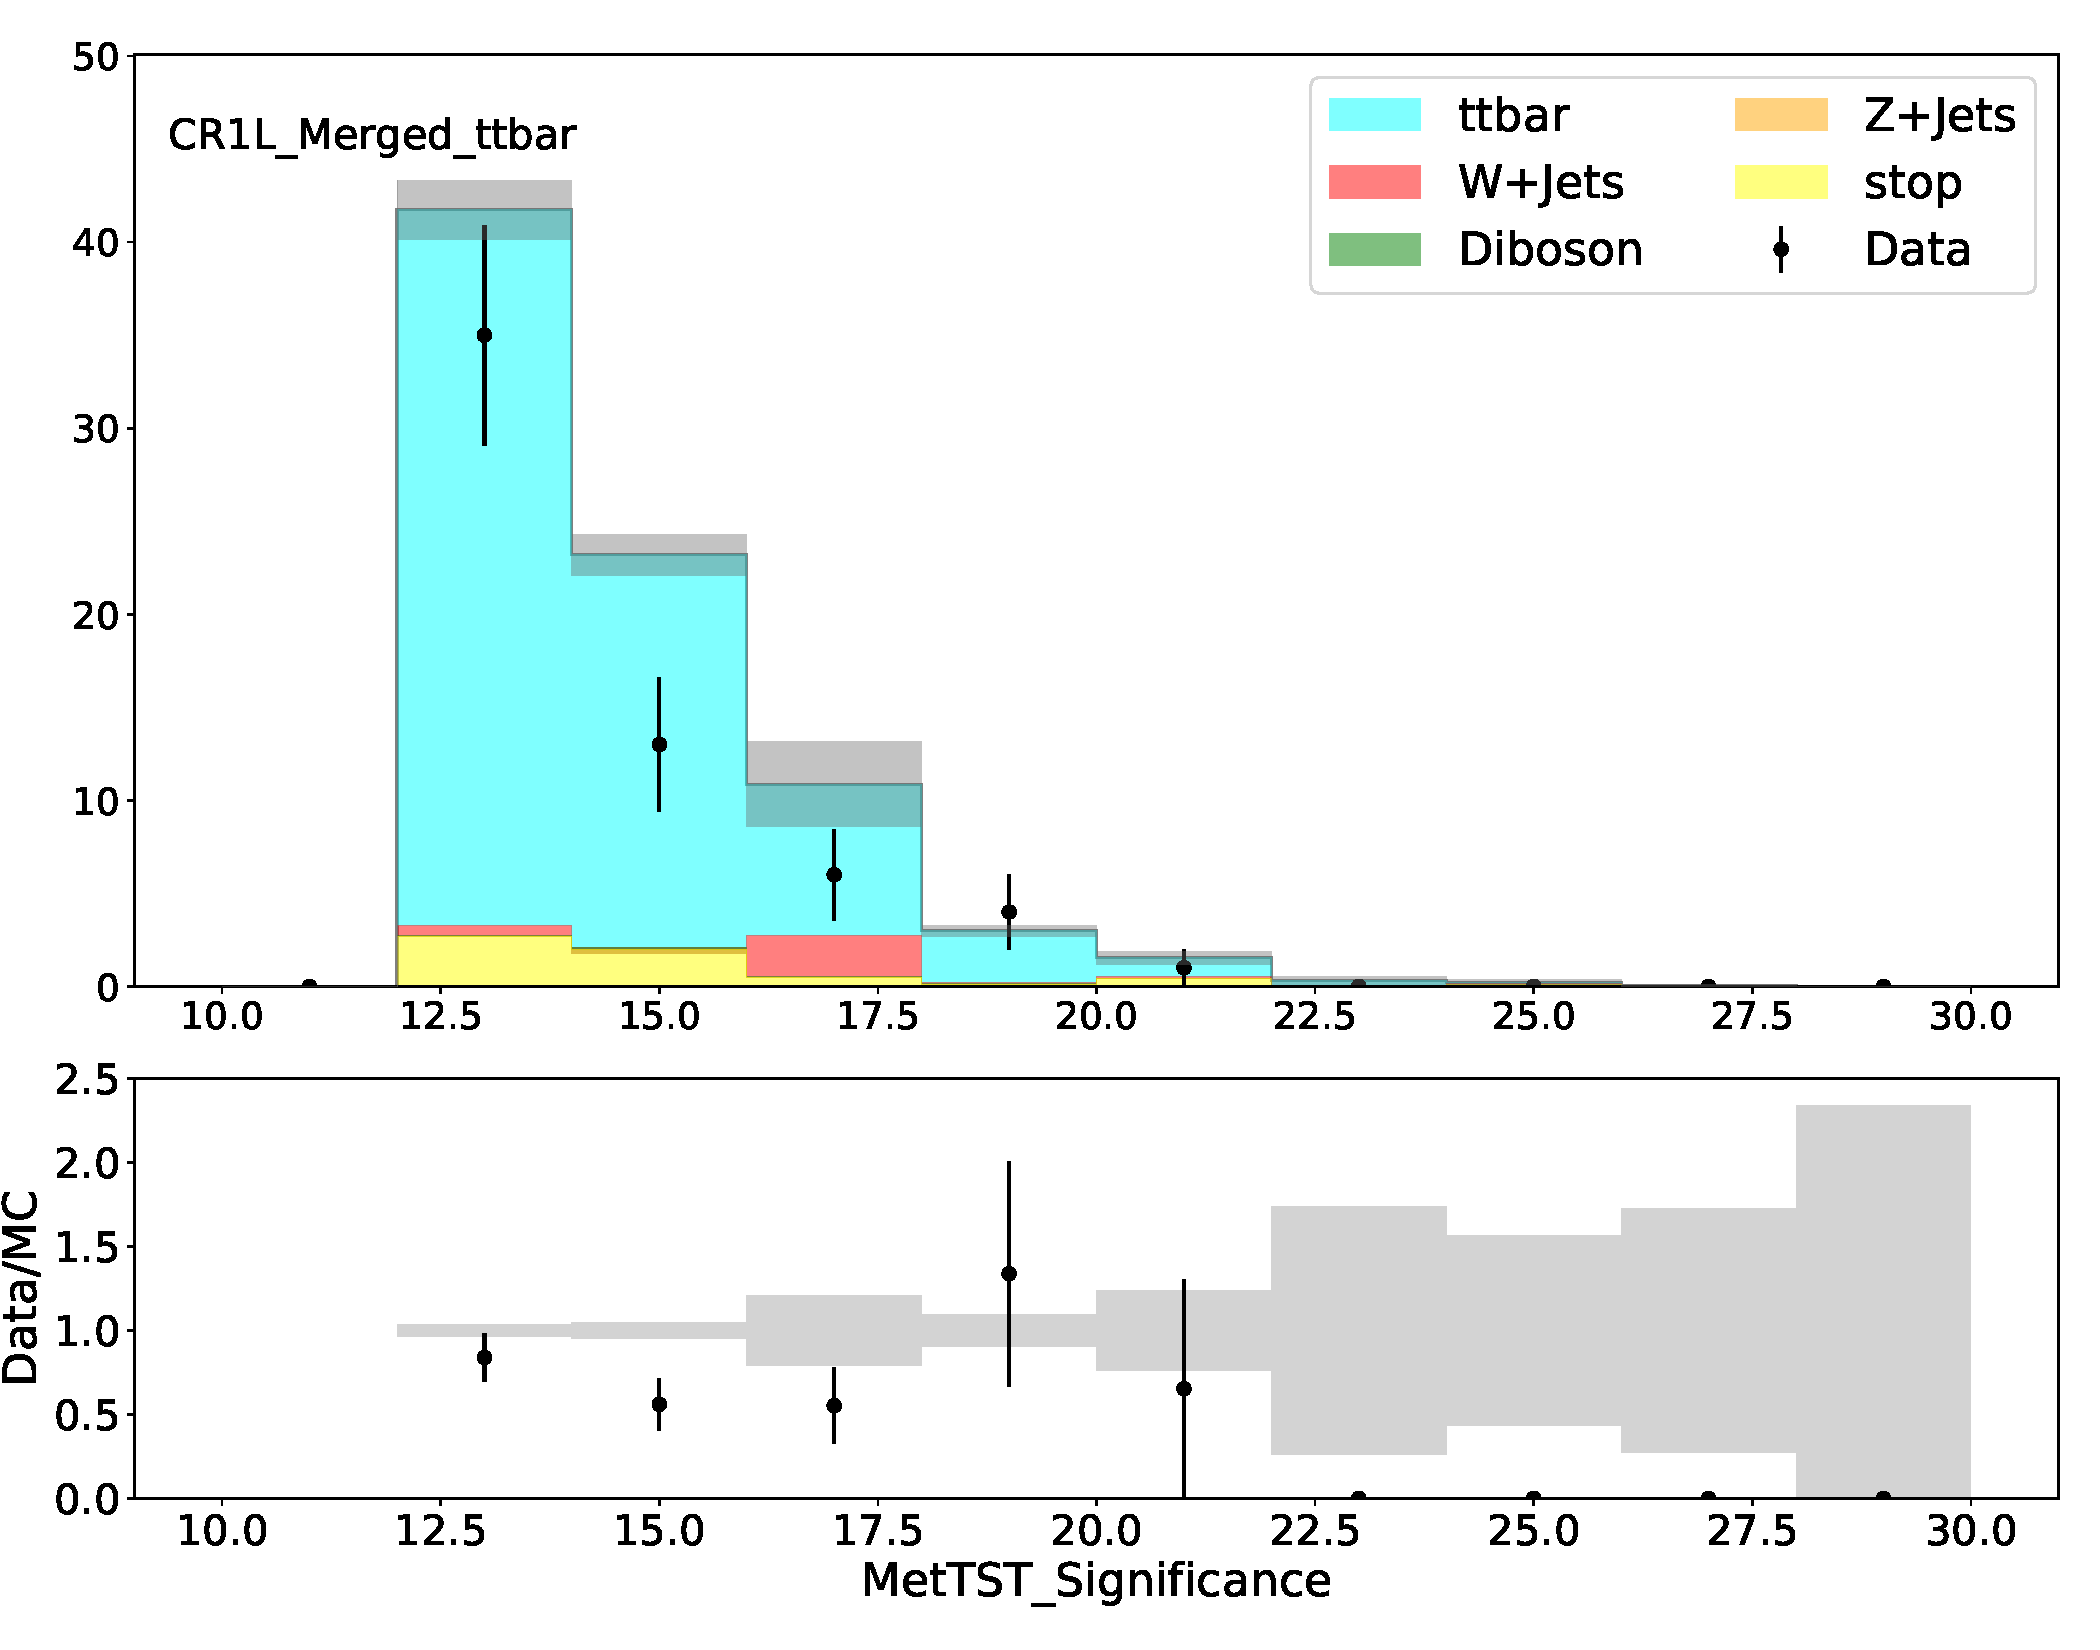
\includegraphics[width = 0.98\textwidth]{Figures/4/datamc/CR1L_Merged_ttbar/MetTST_Significance.pdf}
     \caption{\metsig}
     \end{subfigure}
     \begin{subfigure}{0.49\textwidth}
     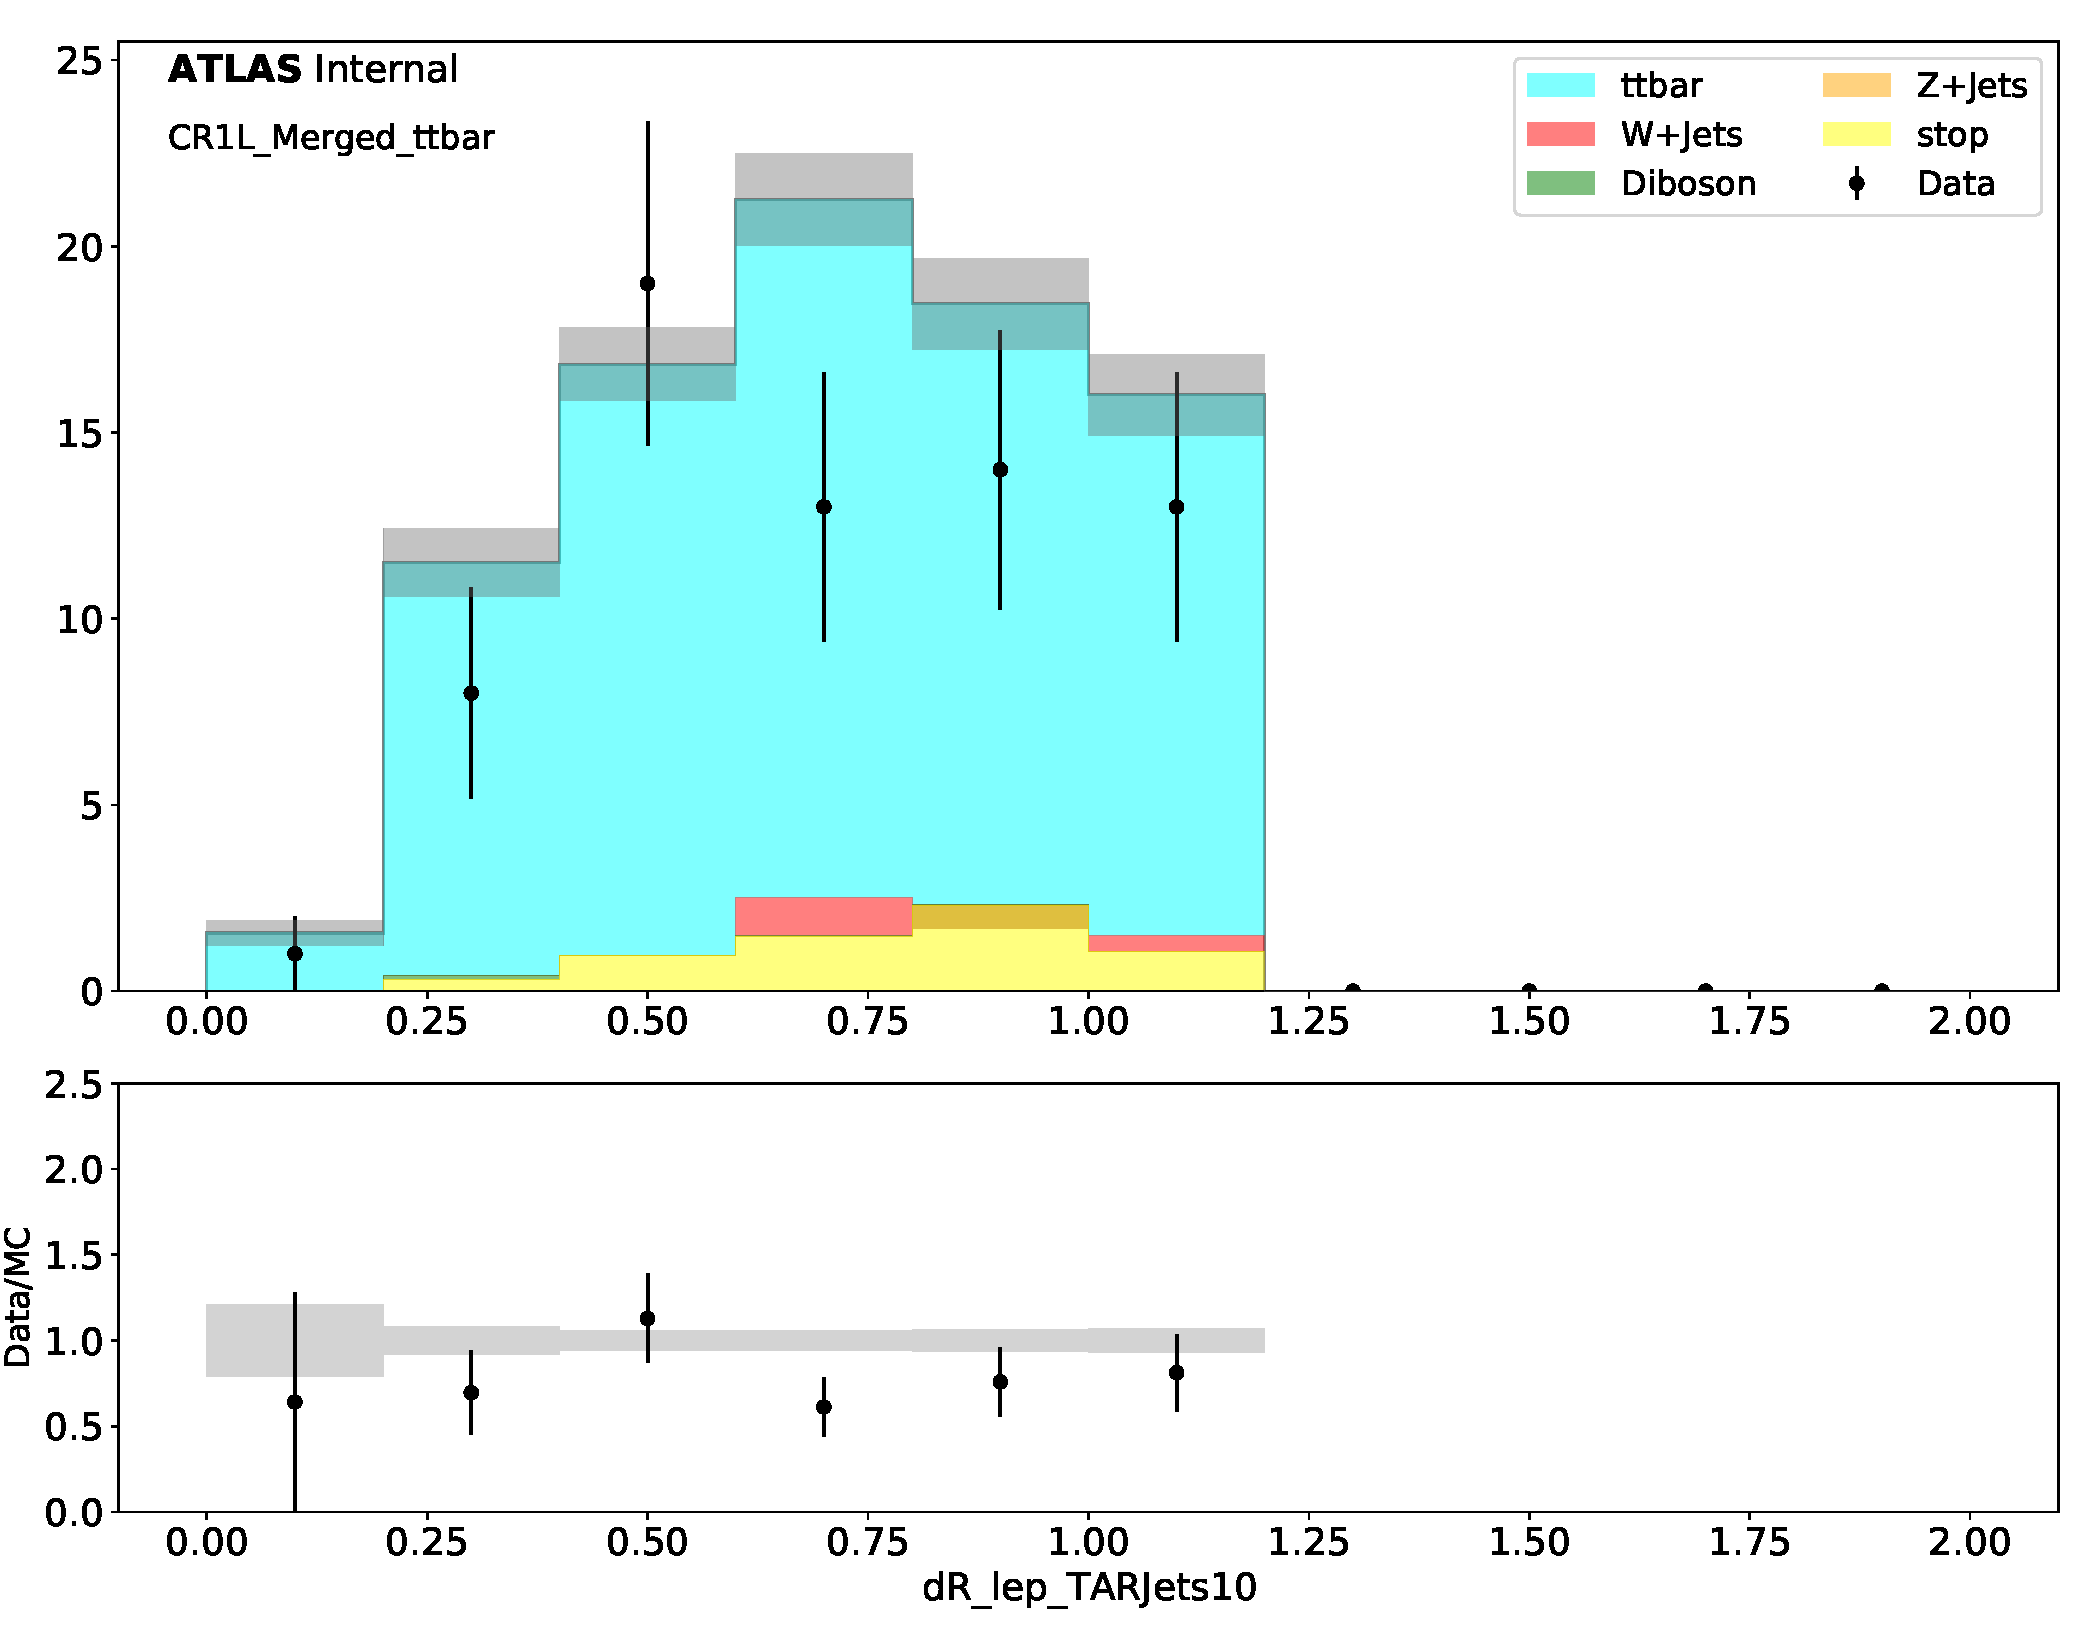
\includegraphics[width = 0.98\textwidth]{Figures/4/datamc/CR1L_Merged_ttbar/dR_lep_TARJets10.pdf}
     \caption{\drTARl}
     \end{subfigure}
     \caption{Data-MC Comparisons in the \merged \ttbar control region. Grey bands represent MC statistical uncertainty on each bin.}
     \label{fig:Data_MC_CRbV_merged}
  \end{figure}

\begin{figure}[htbp]
  \centering
     \begin{subfigure}{0.49\textwidth}
     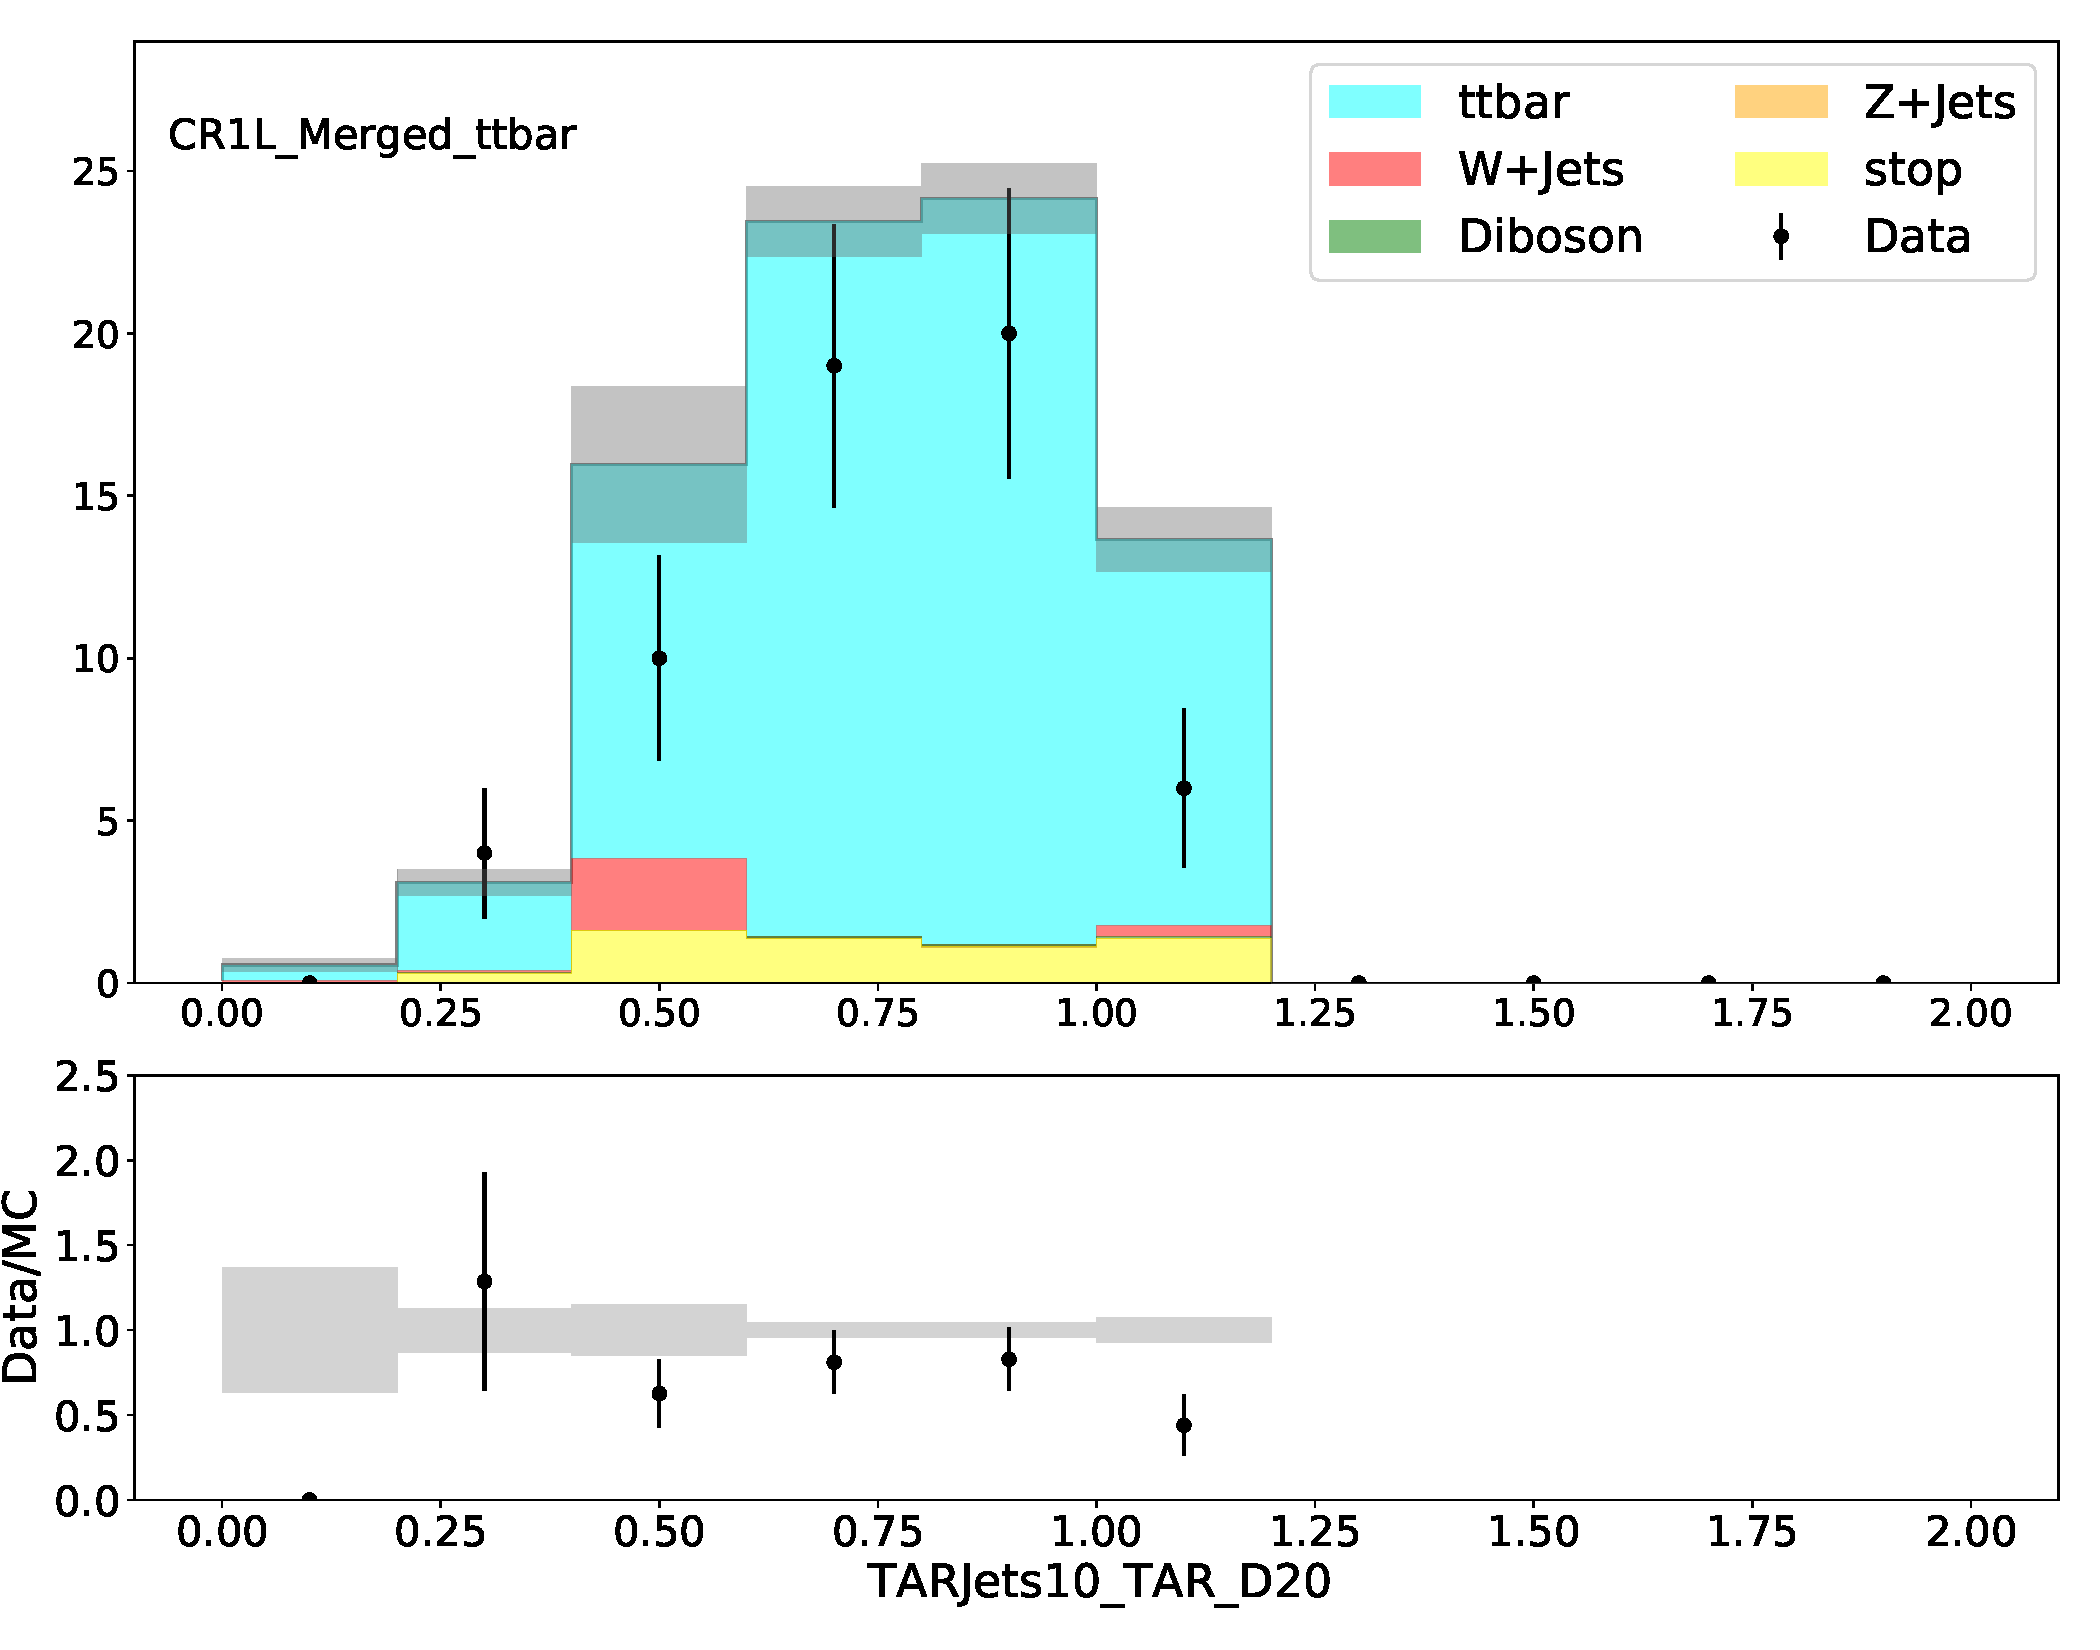
\includegraphics[width = 0.98\textwidth]{Figures/4/datamc/CR1L_Merged_ttbar/TARJets10_TAR_D20.pdf}
     \caption{\DtwoTAR}
     \end{subfigure}
     \begin{subfigure}{0.49\textwidth}
     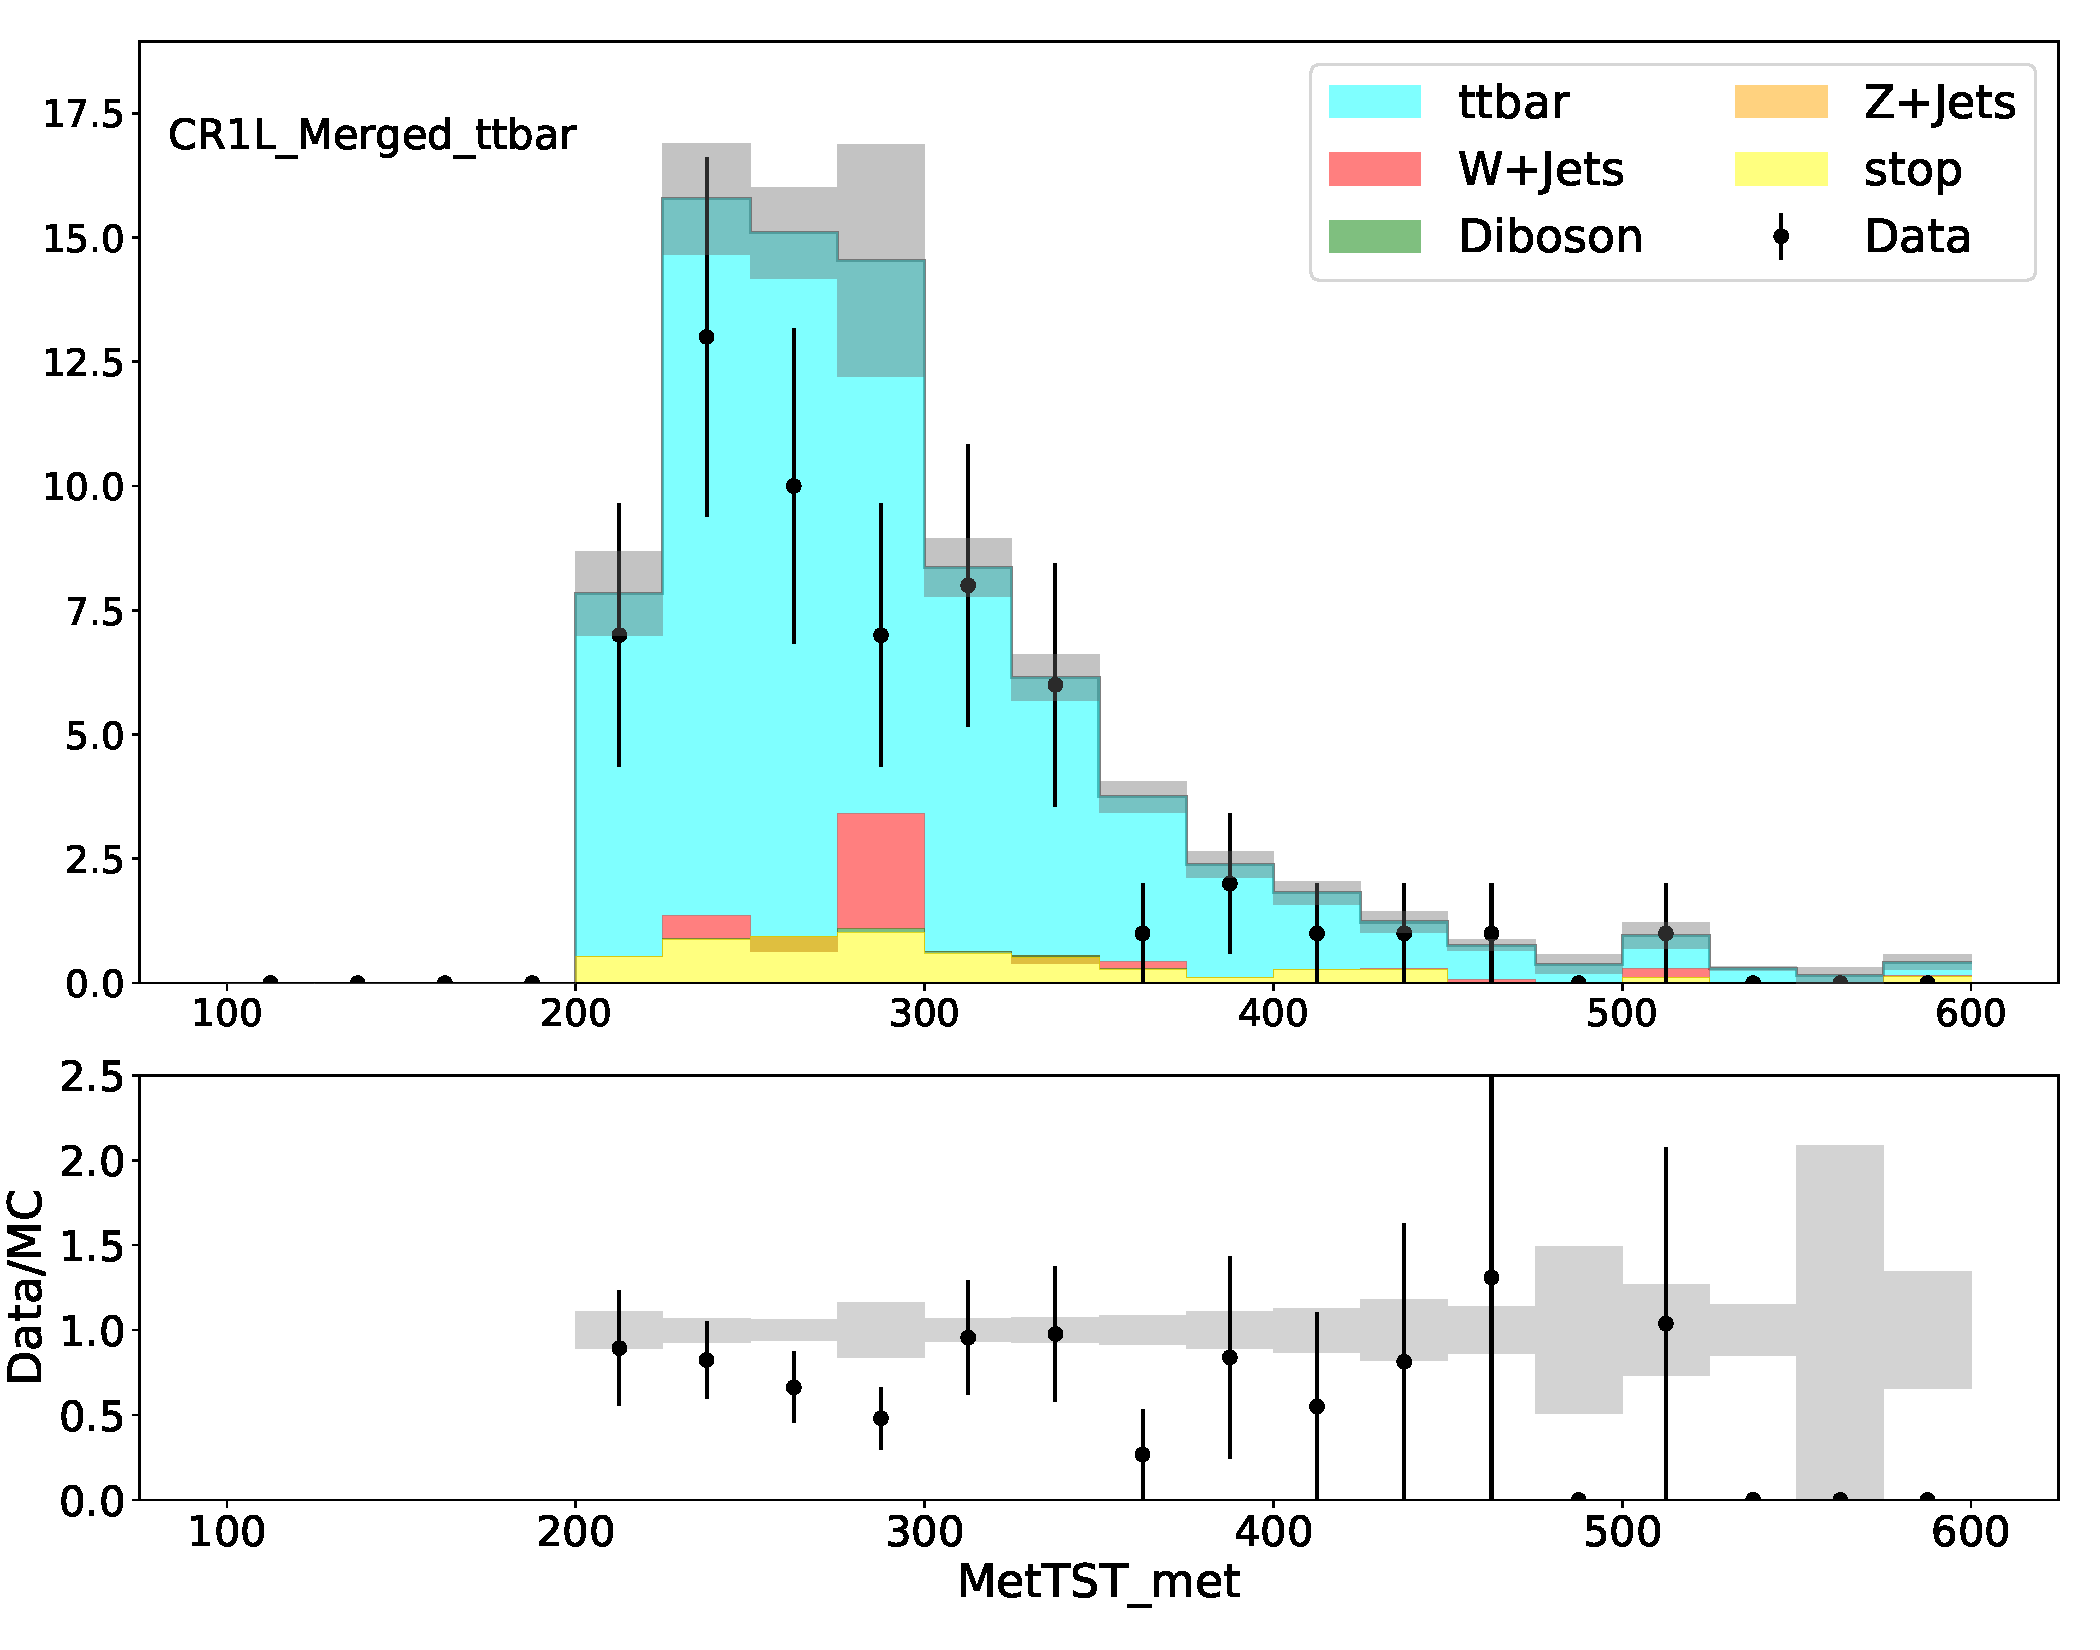
\includegraphics[width = 0.98\textwidth]{Figures/4/datamc/CR1L_Merged_ttbar/MetTST_met.pdf}
     \caption{\met}
     \end{subfigure}

     \caption{Data-MC Comparisons in the \merged \ttbar control region. Grey bands represent MC statistical uncertainty on each bin.}
     \label{fig:Data_MC_CRbV_merged}
  \end{figure}

\begin{figure}[htbp]
  \centering
     \begin{subfigure}{0.49\textwidth}
     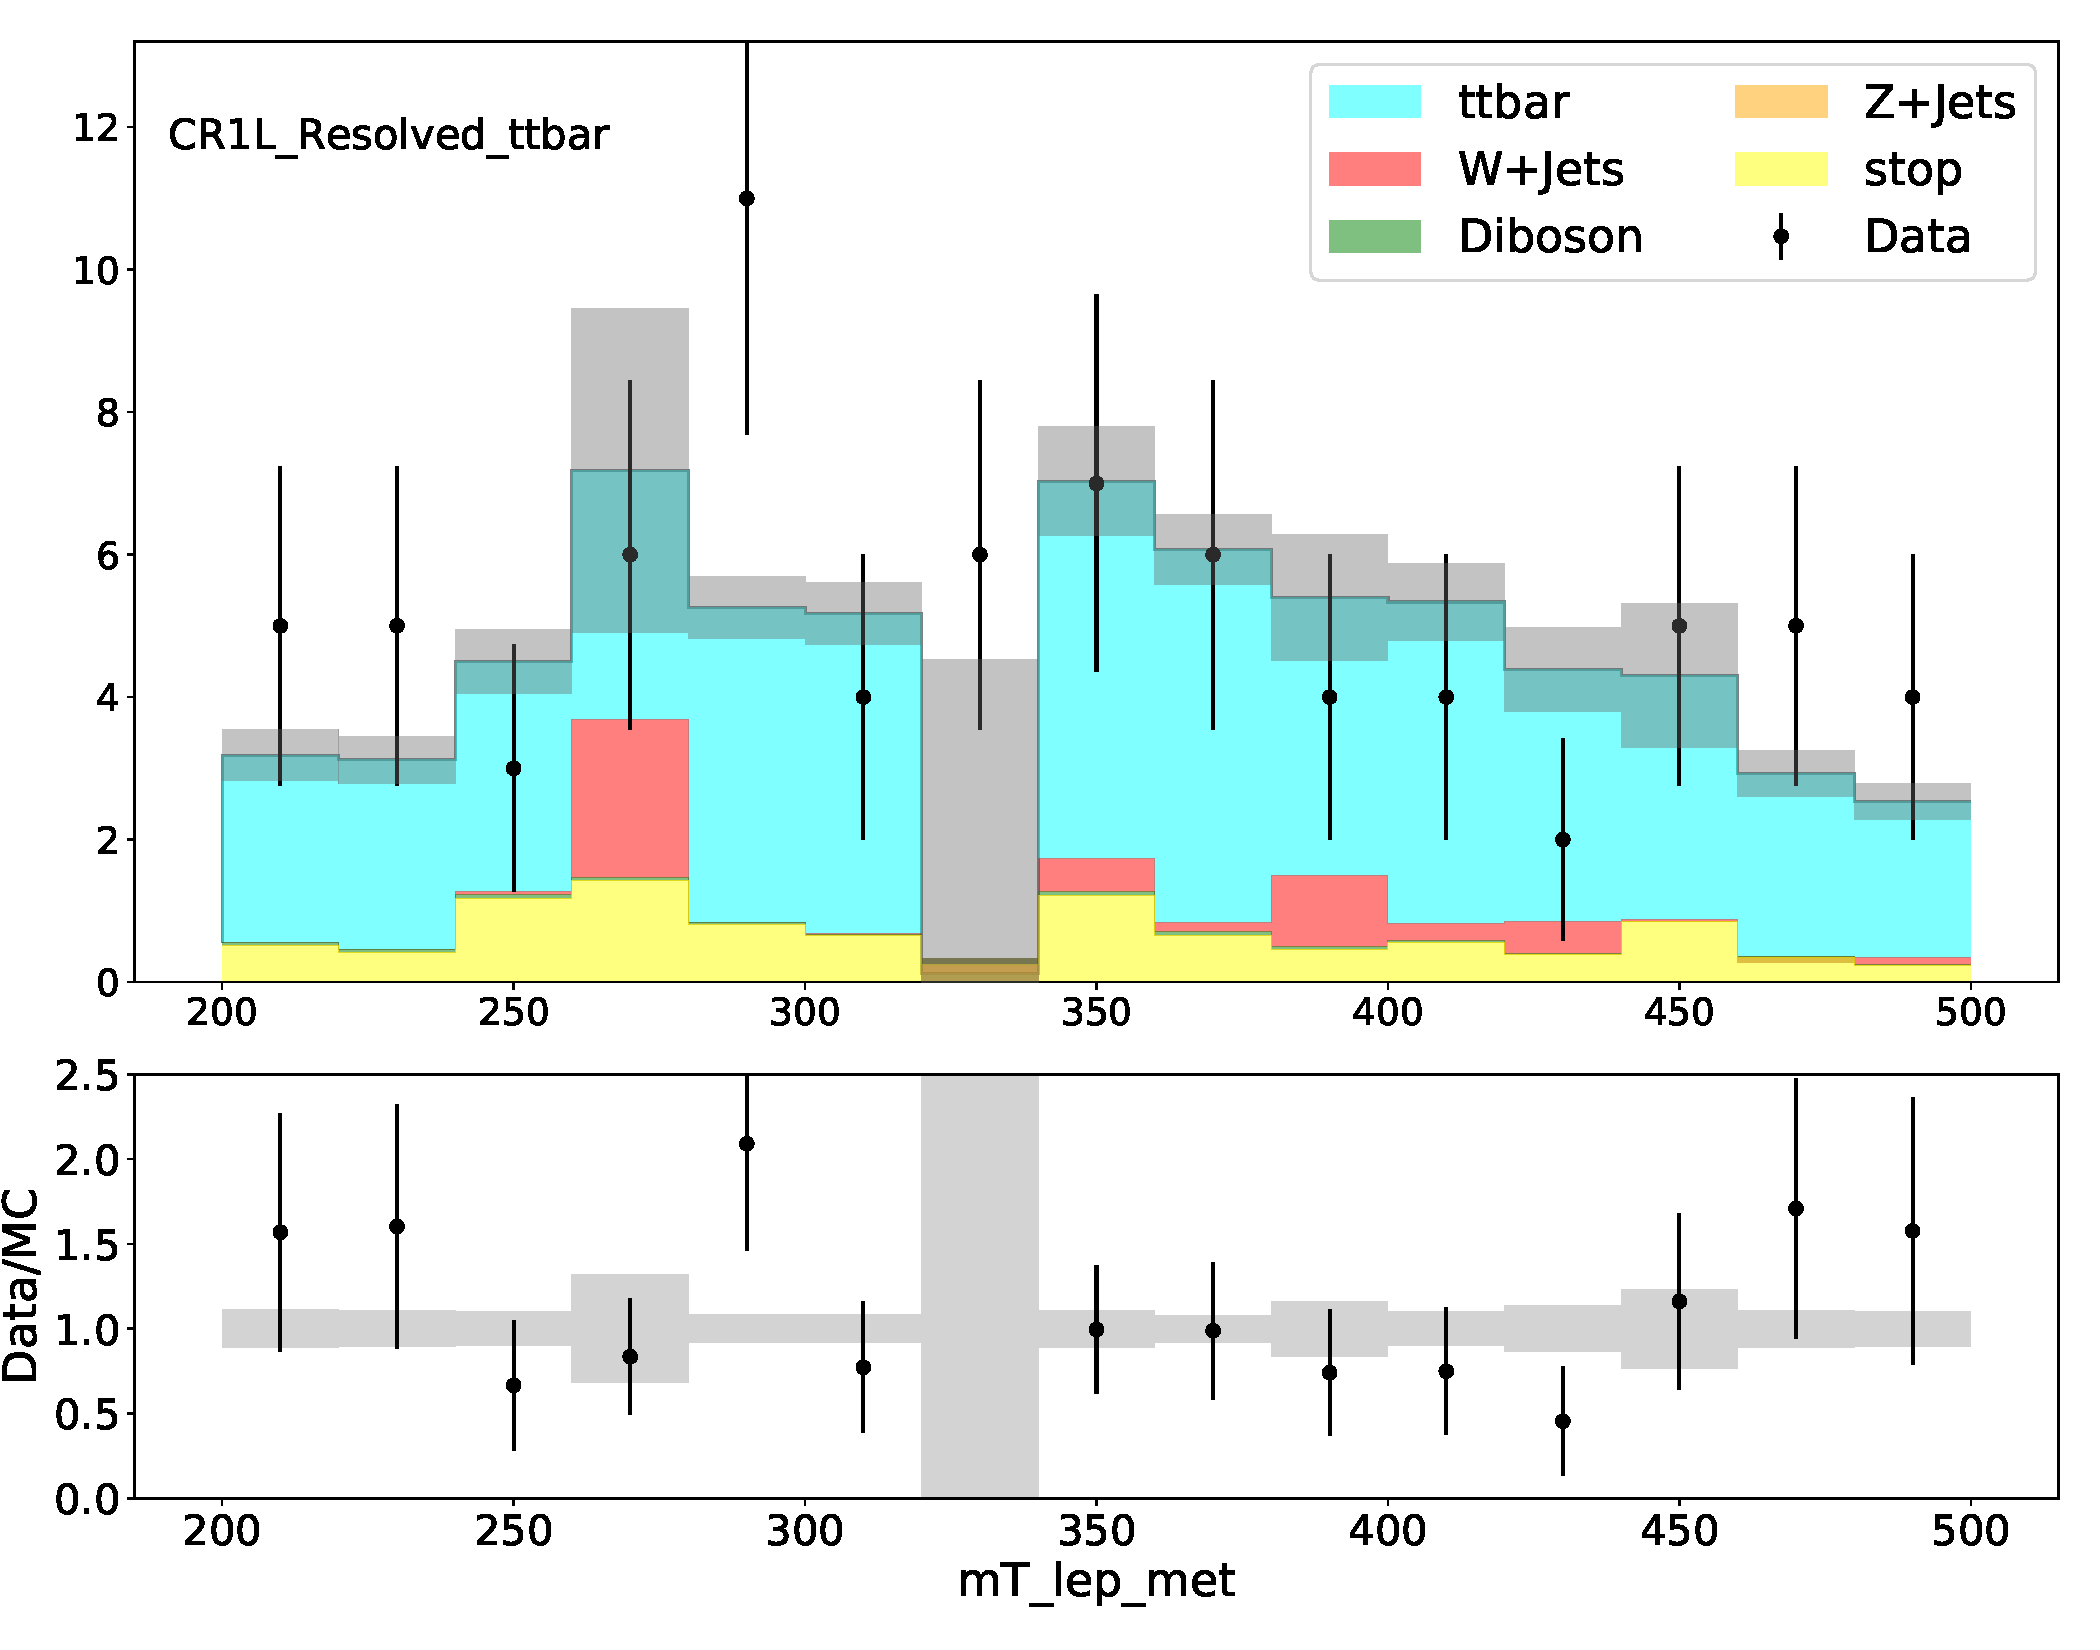
\includegraphics[width = 0.98\textwidth]{Figures/4/datamc/CR1L_Resolved_ttbar/mT_lep_met.pdf}
     \caption{\mtlepmet}
     \end{subfigure}
     \begin{subfigure}{0.49\textwidth}
     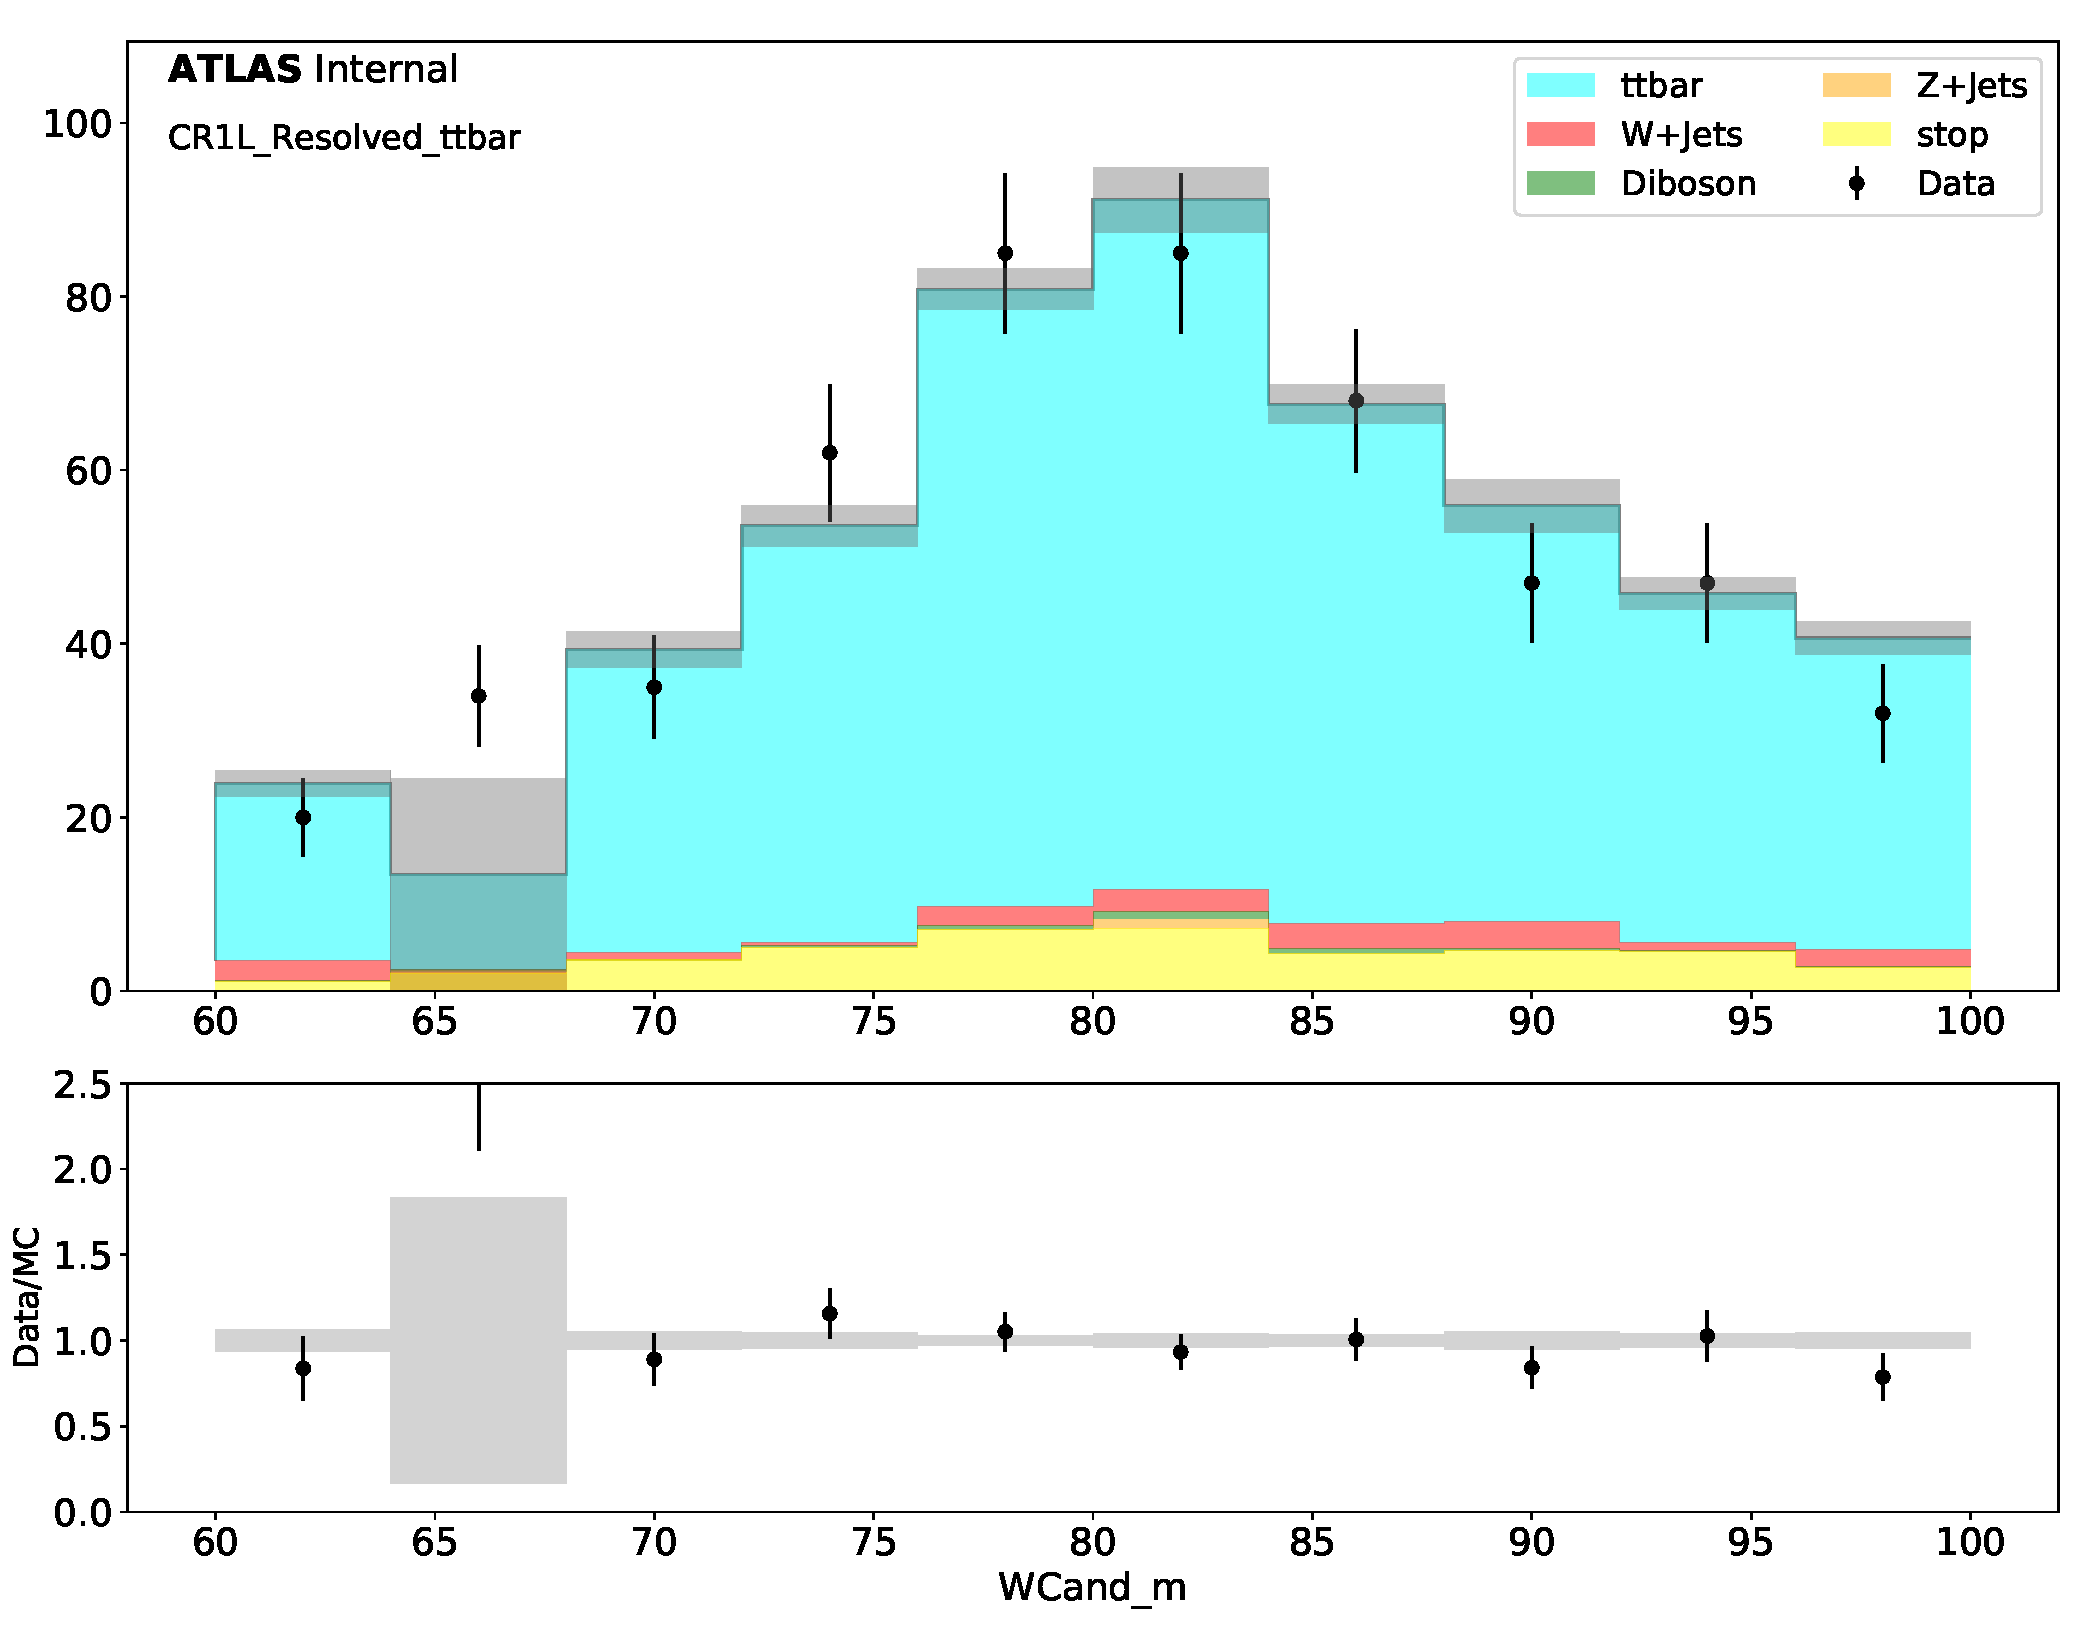
\includegraphics[width = 0.98\textwidth]{Figures/4/datamc/CR1L_Resolved_ttbar/WCand_m.pdf}
     \caption{\Wcandm}
     \end{subfigure}
     \begin{subfigure}{0.49\textwidth}
     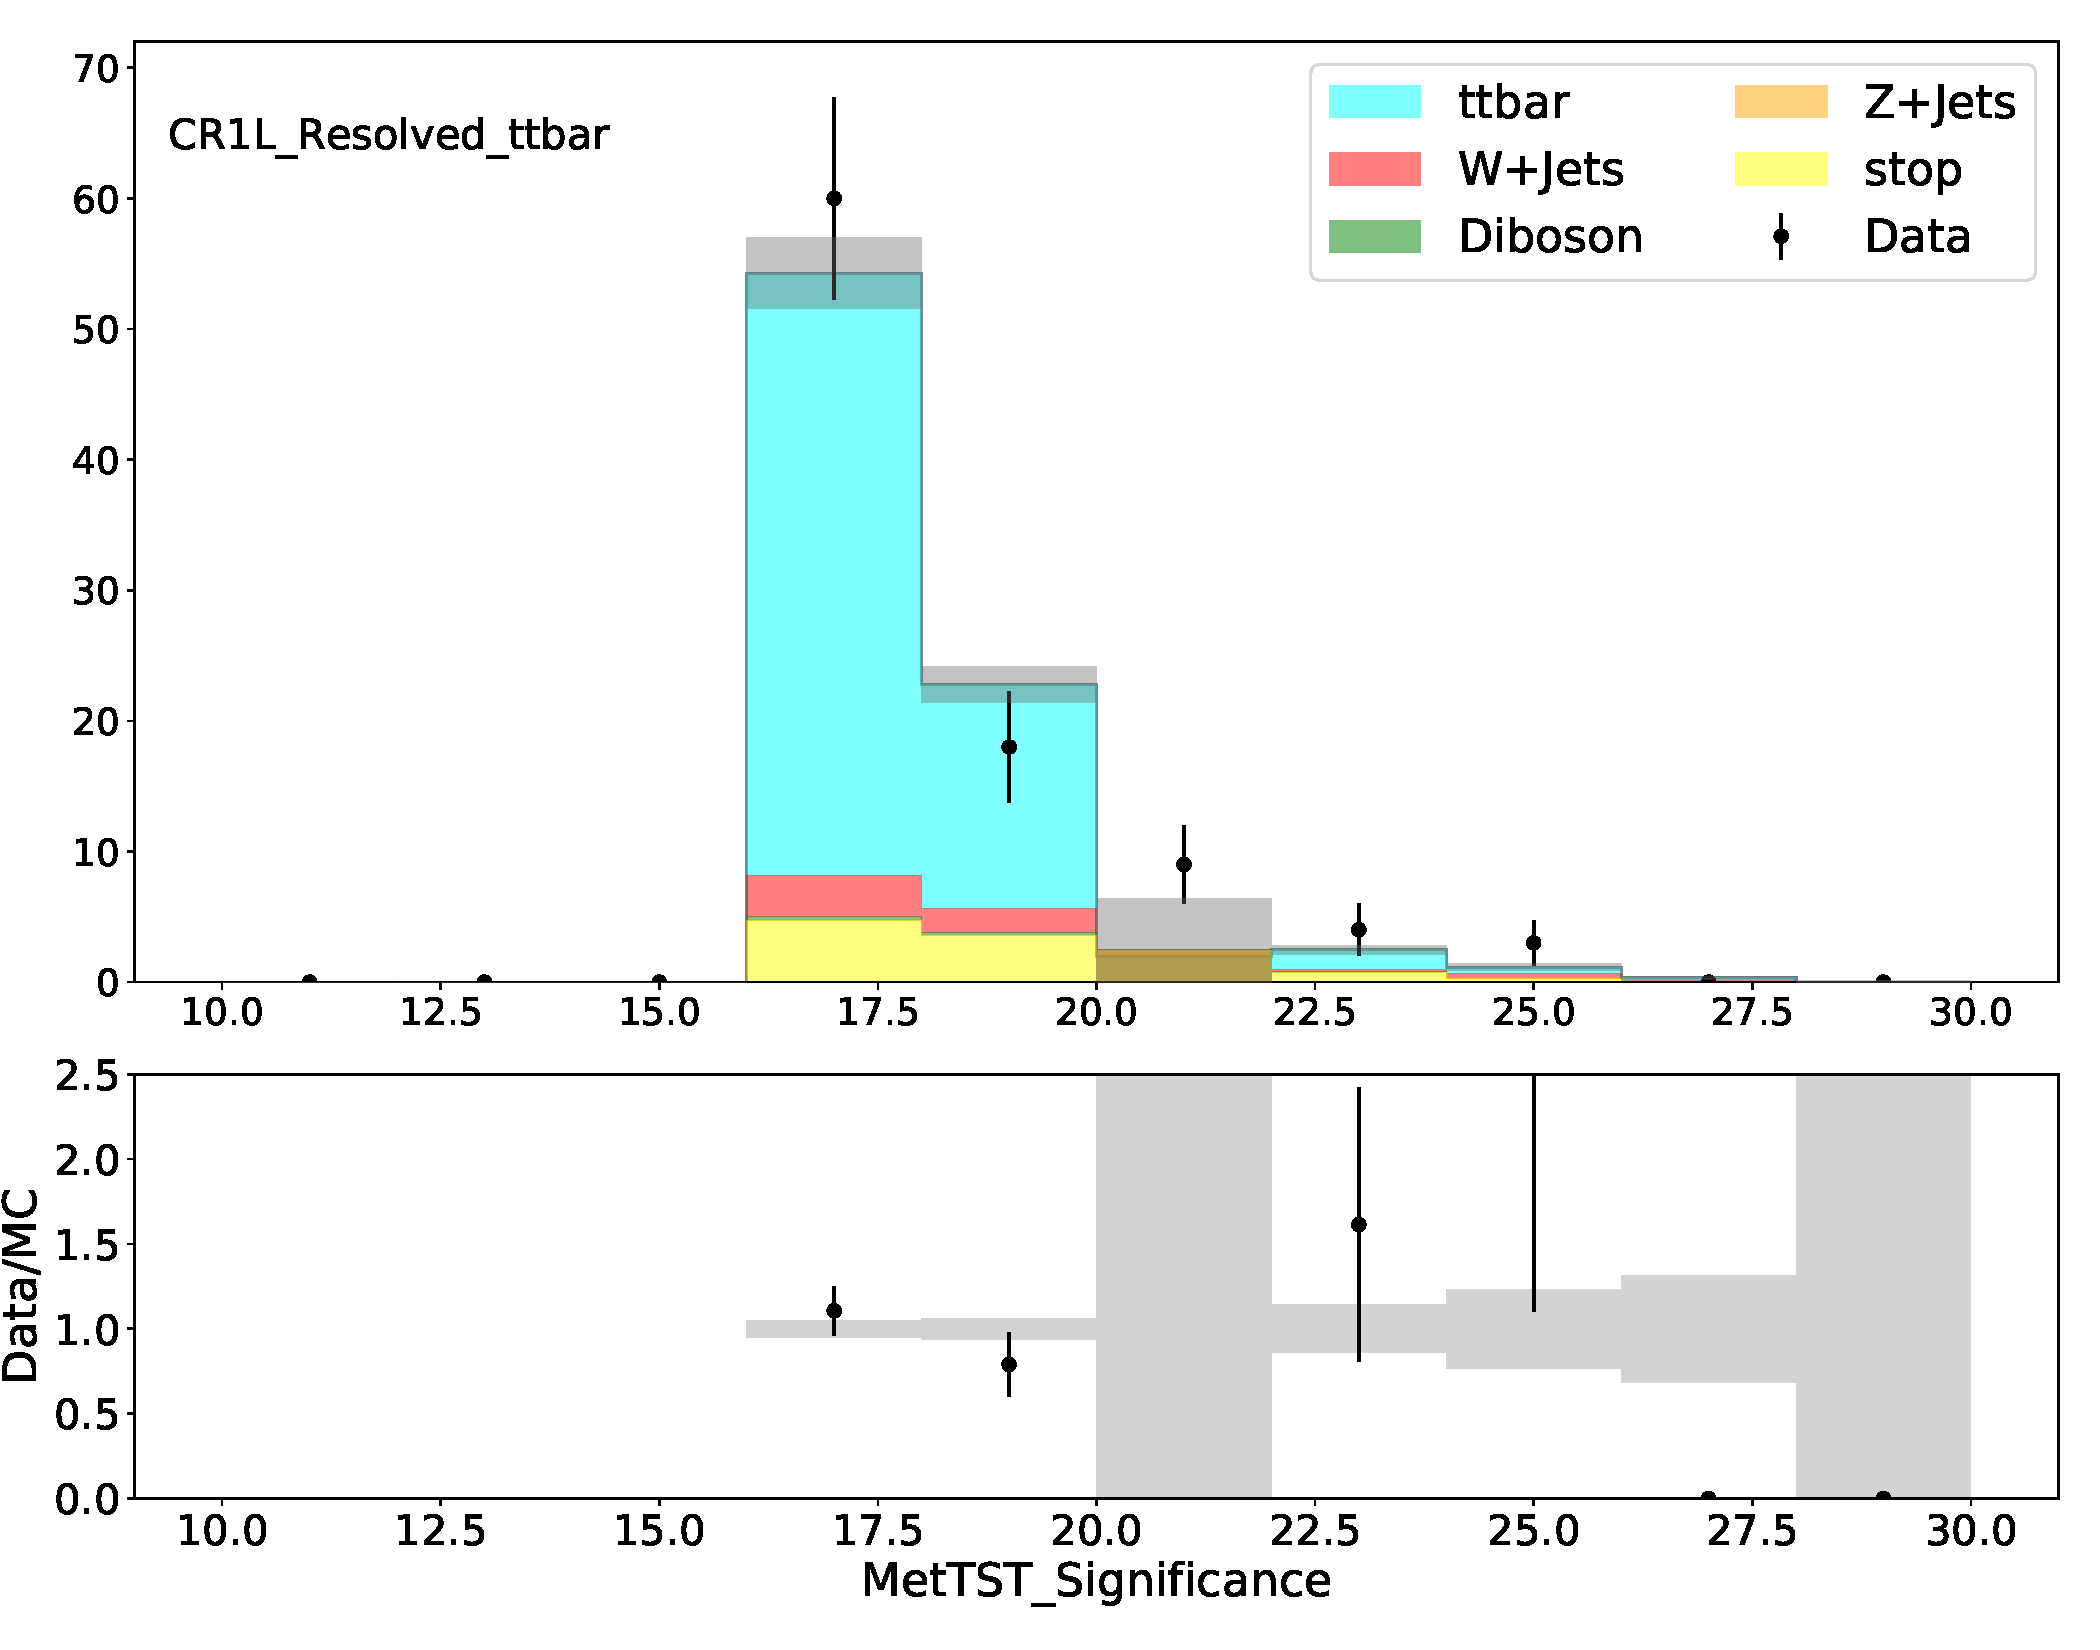
\includegraphics[width = 0.98\textwidth]{Figures/4/datamc/CR1L_Resolved_ttbar/MetTST_Significance.pdf}
     \caption{\metsig}
     \end{subfigure}
     \begin{subfigure}{0.49\textwidth}
     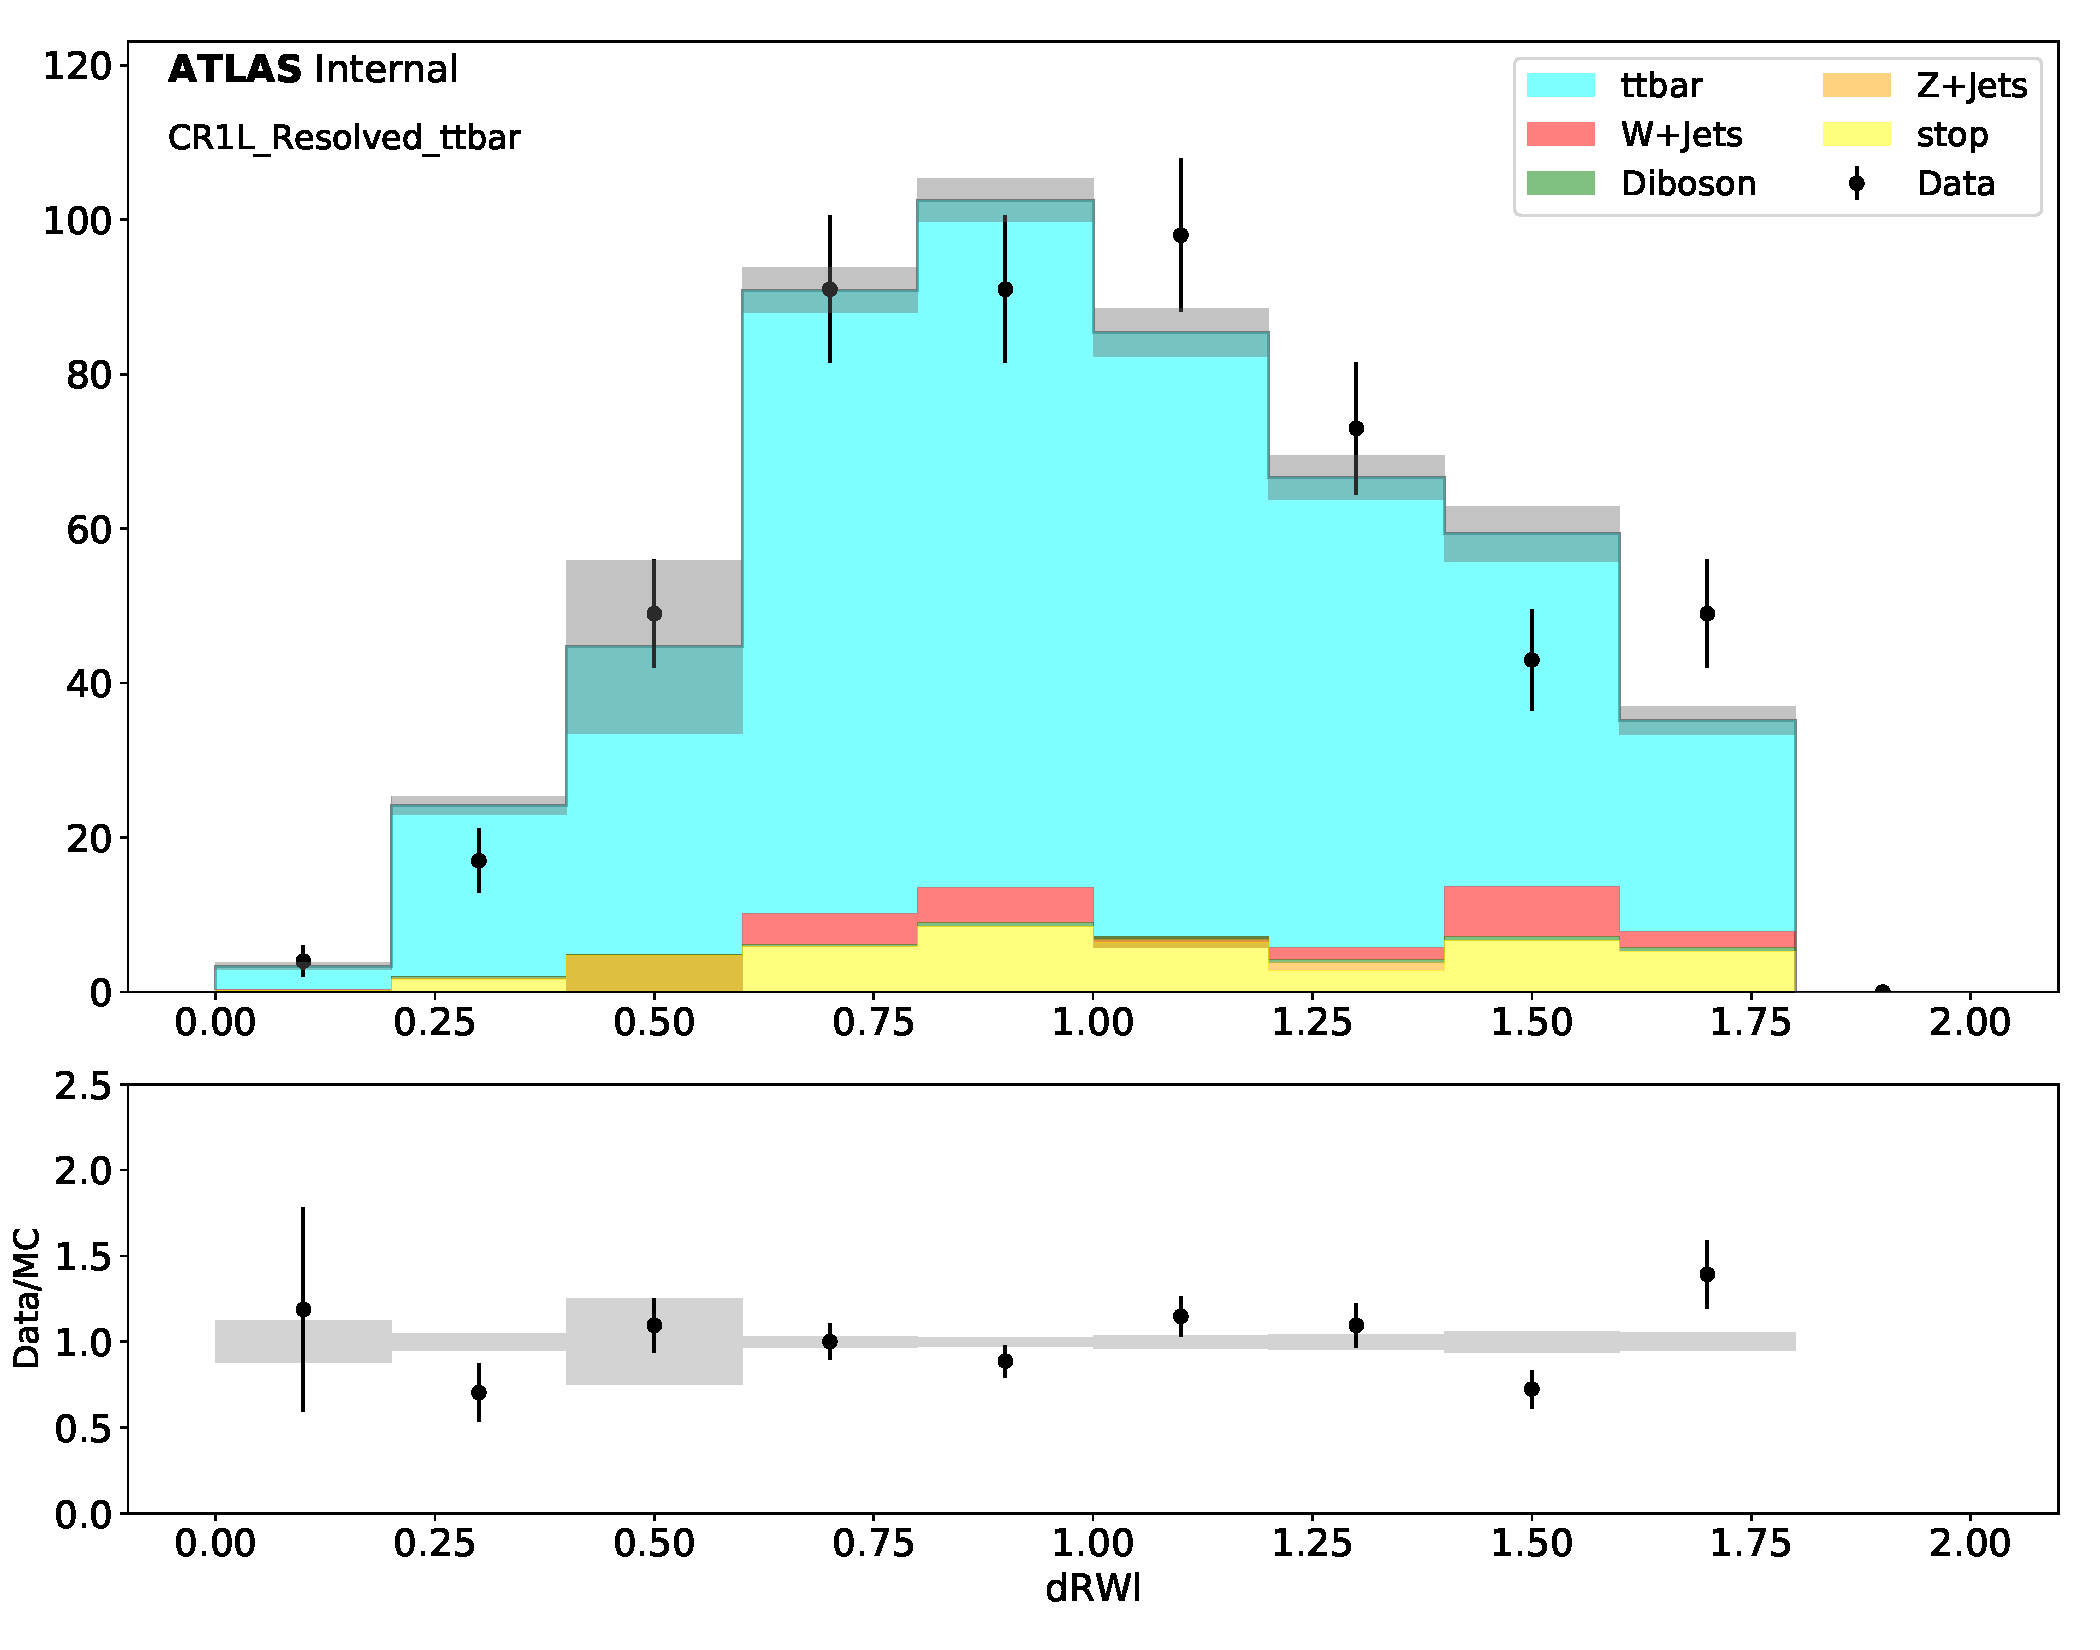
\includegraphics[width = 0.98\textwidth]{Figures/4/datamc/CR1L_Resolved_ttbar/dRWl.pdf}
     \caption{\drWl}
     \end{subfigure}
     \caption{Data-MC Comparisons in the \resolved \ttbar control region. Grey bands represent MC statistical uncertainty on each bin.}
     \label{fig:Data_MC_CRbV_resolved}
     \end{figure}

     \begin{figure}[htbp]
    \centering
     \begin{subfigure}{0.49\textwidth}
     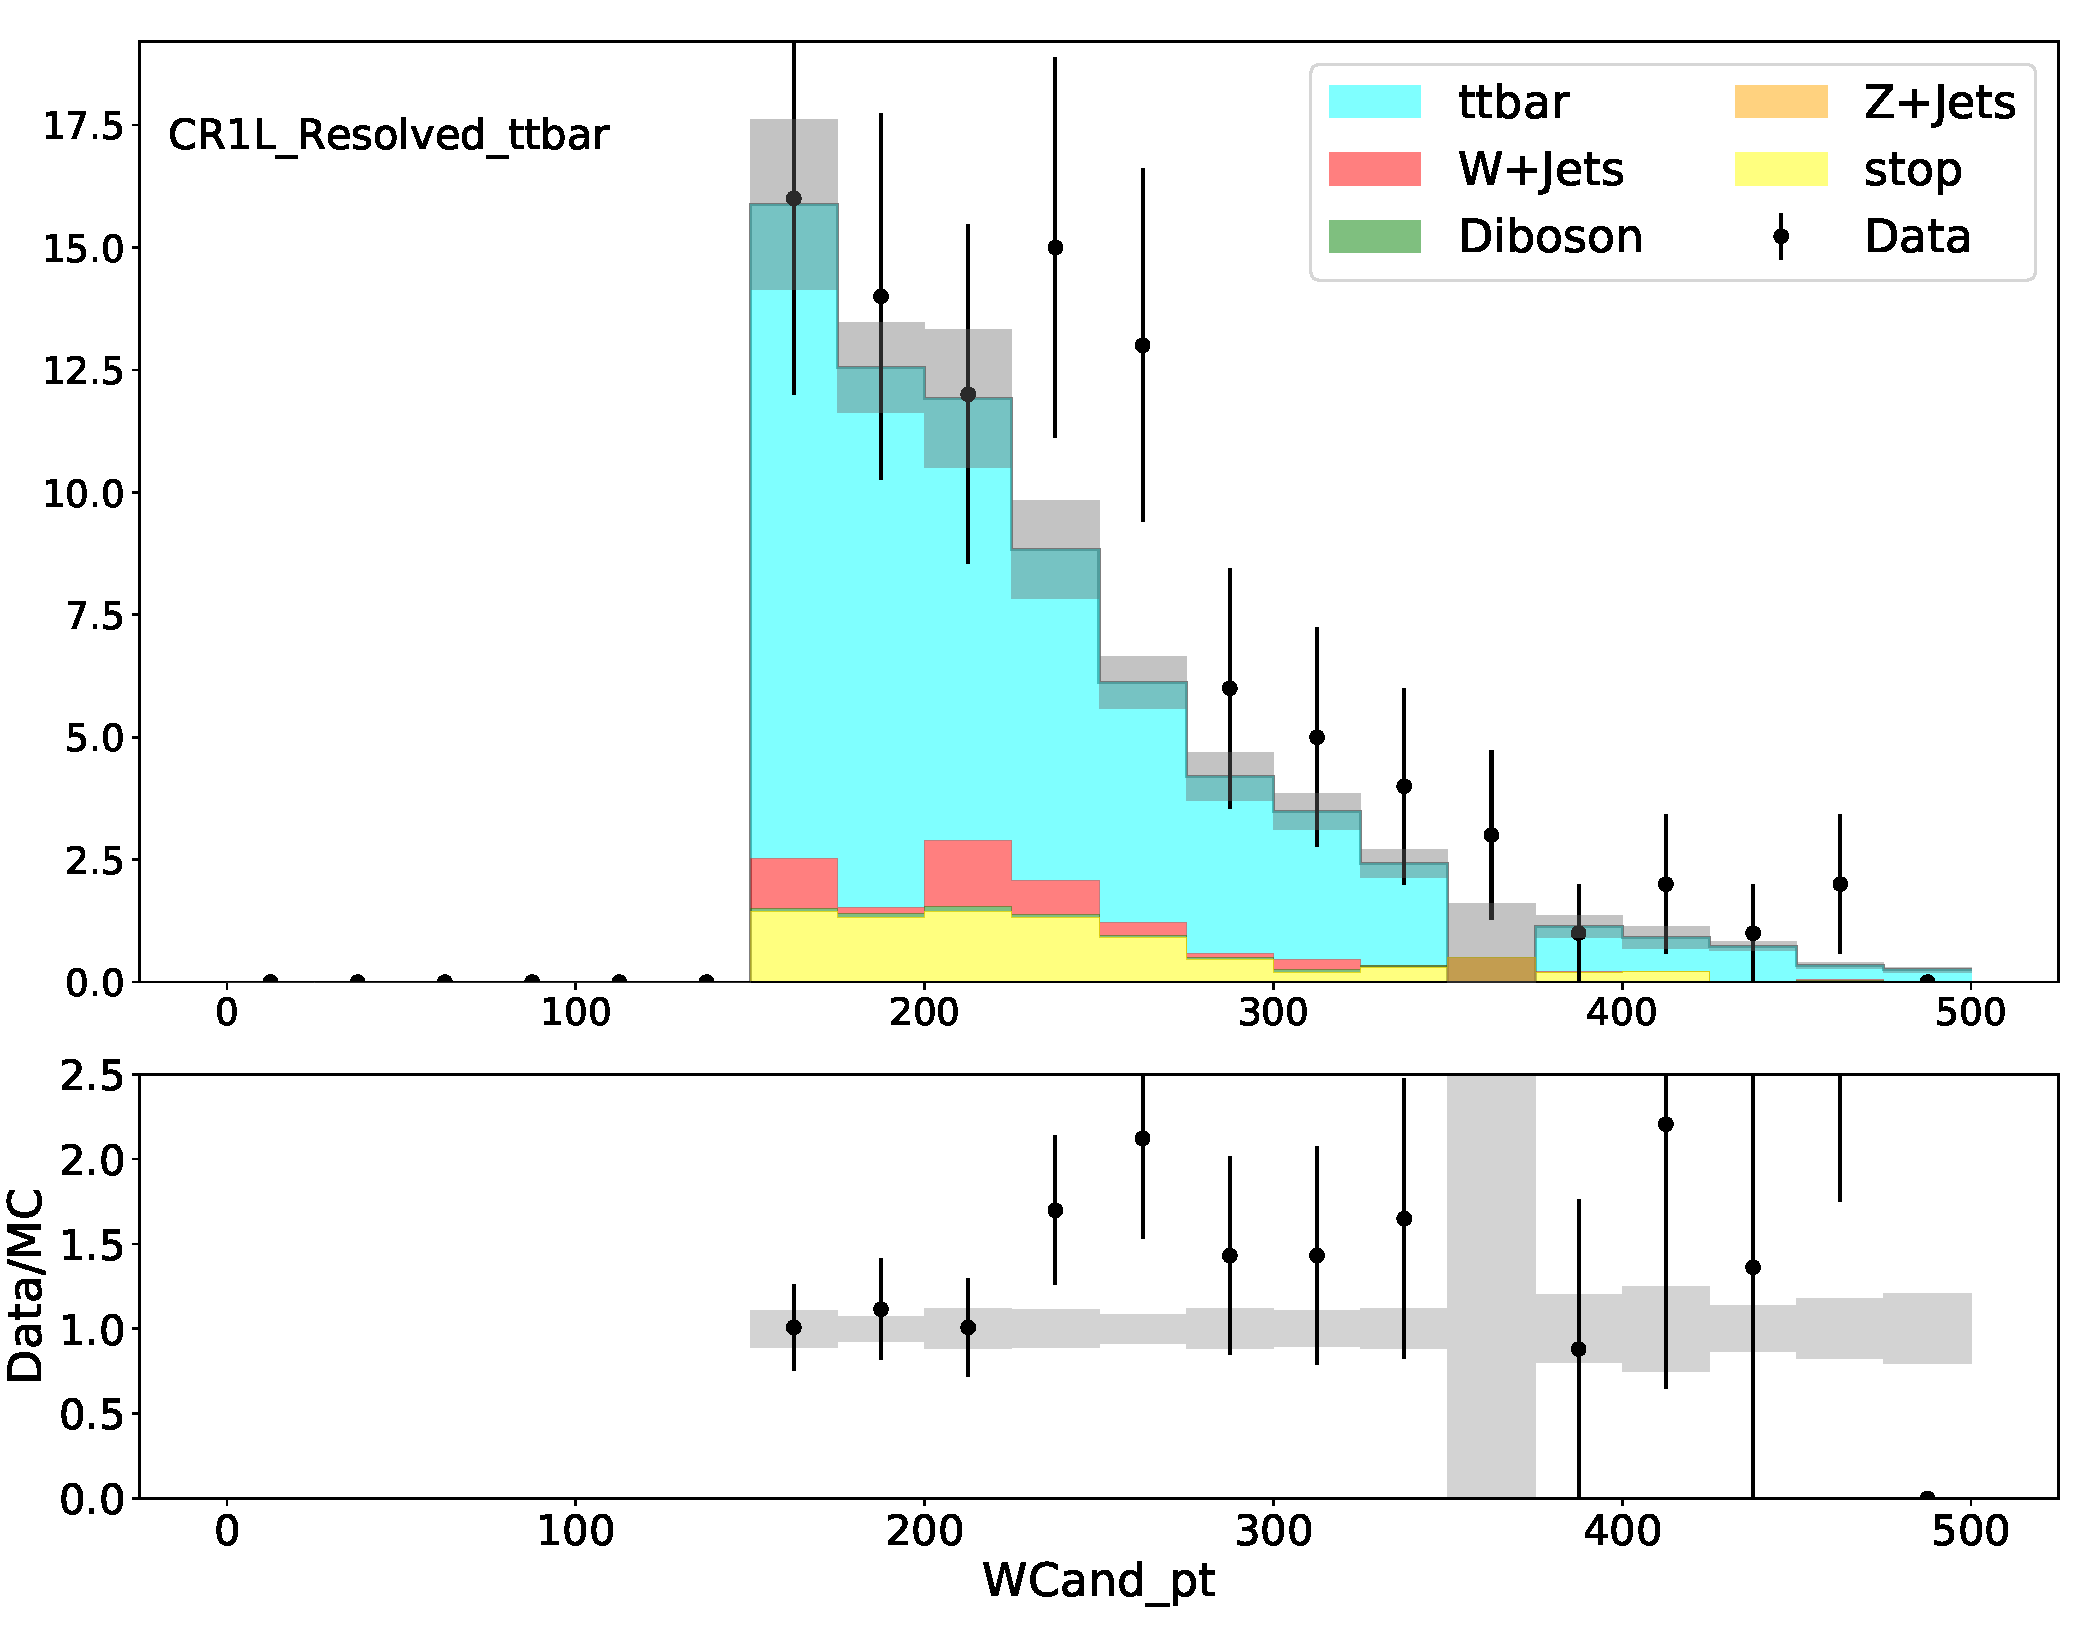
\includegraphics[width = 0.98\textwidth]{Figures/4/datamc/CR1L_Resolved_ttbar/WCand_pt.pdf}
     \caption{\Wcandpt}
     \end{subfigure}
     \begin{subfigure}{0.49\textwidth}
     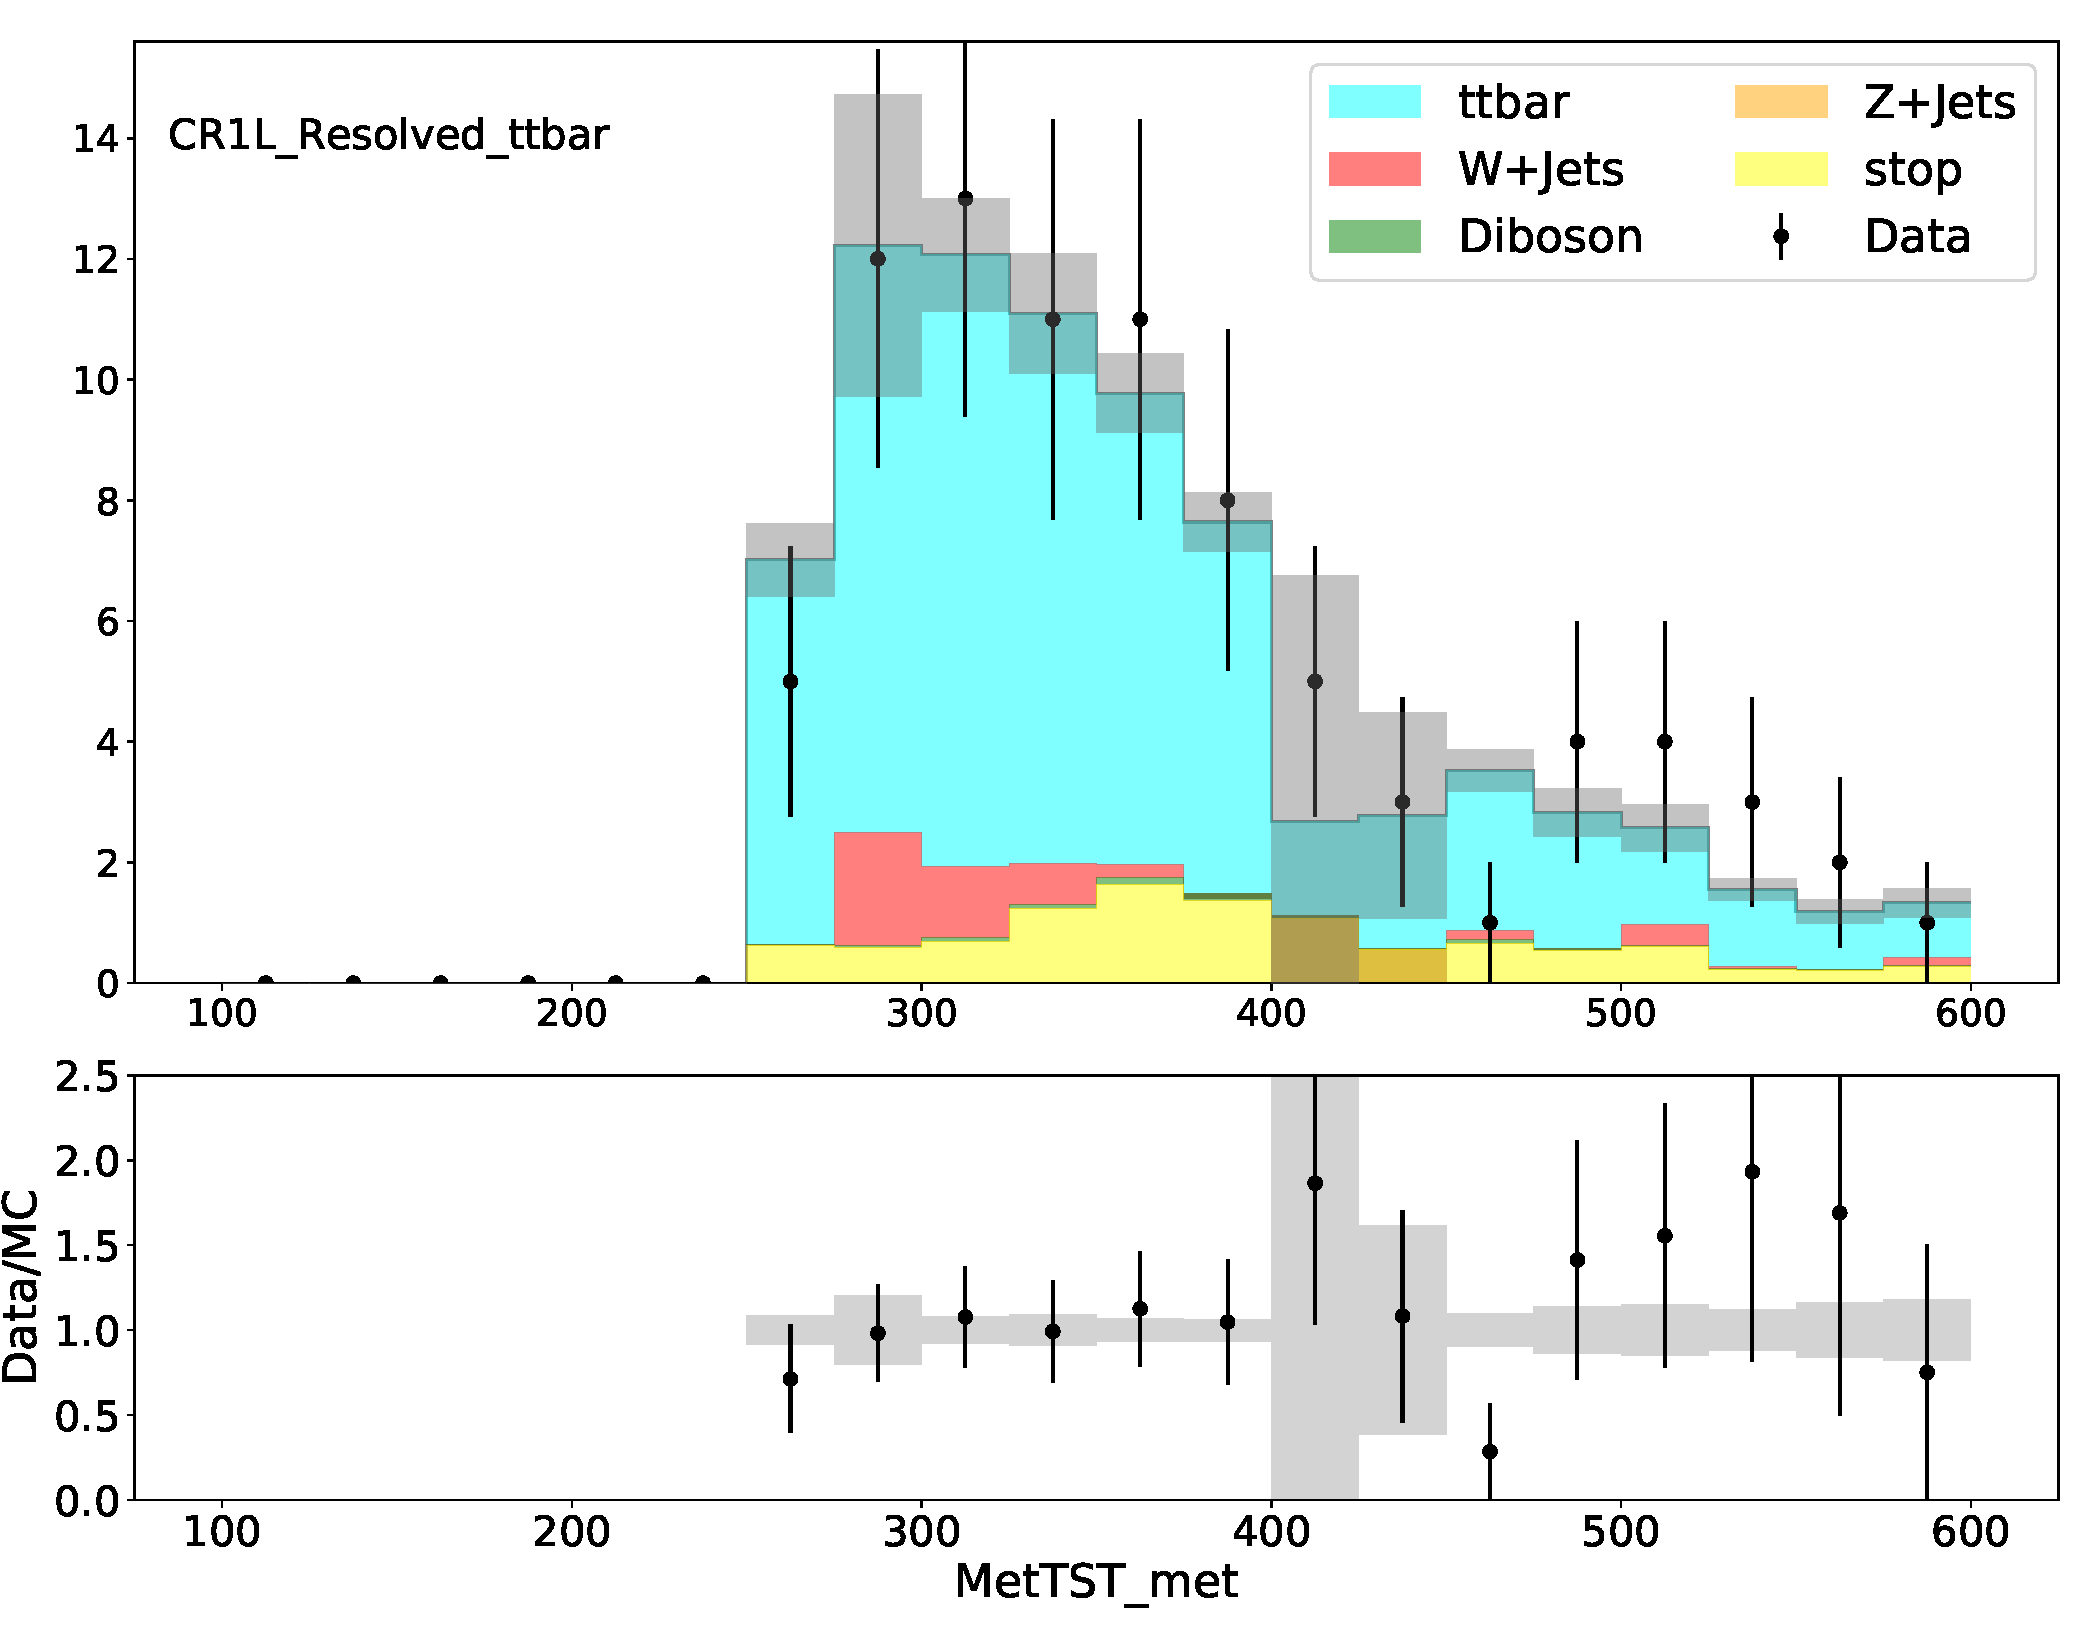
\includegraphics[width = 0.98\textwidth]{Figures/4/datamc/CR1L_Resolved_ttbar/MetTST_met.pdf}
     \caption{\met}
     \end{subfigure}

\caption{Data-MC Comparisons in the \resolved \ttbar control region. Grey bands represent MC statistical uncertainty on each bin.}
\label{fig:Data_MC_CRbV_resolved}
\end{figure}
\FloatBarrier
\subsection{\wjets Control Regions}
\begin{figure}[htbp]
  \centering
     \begin{subfigure}{0.49\textwidth}
     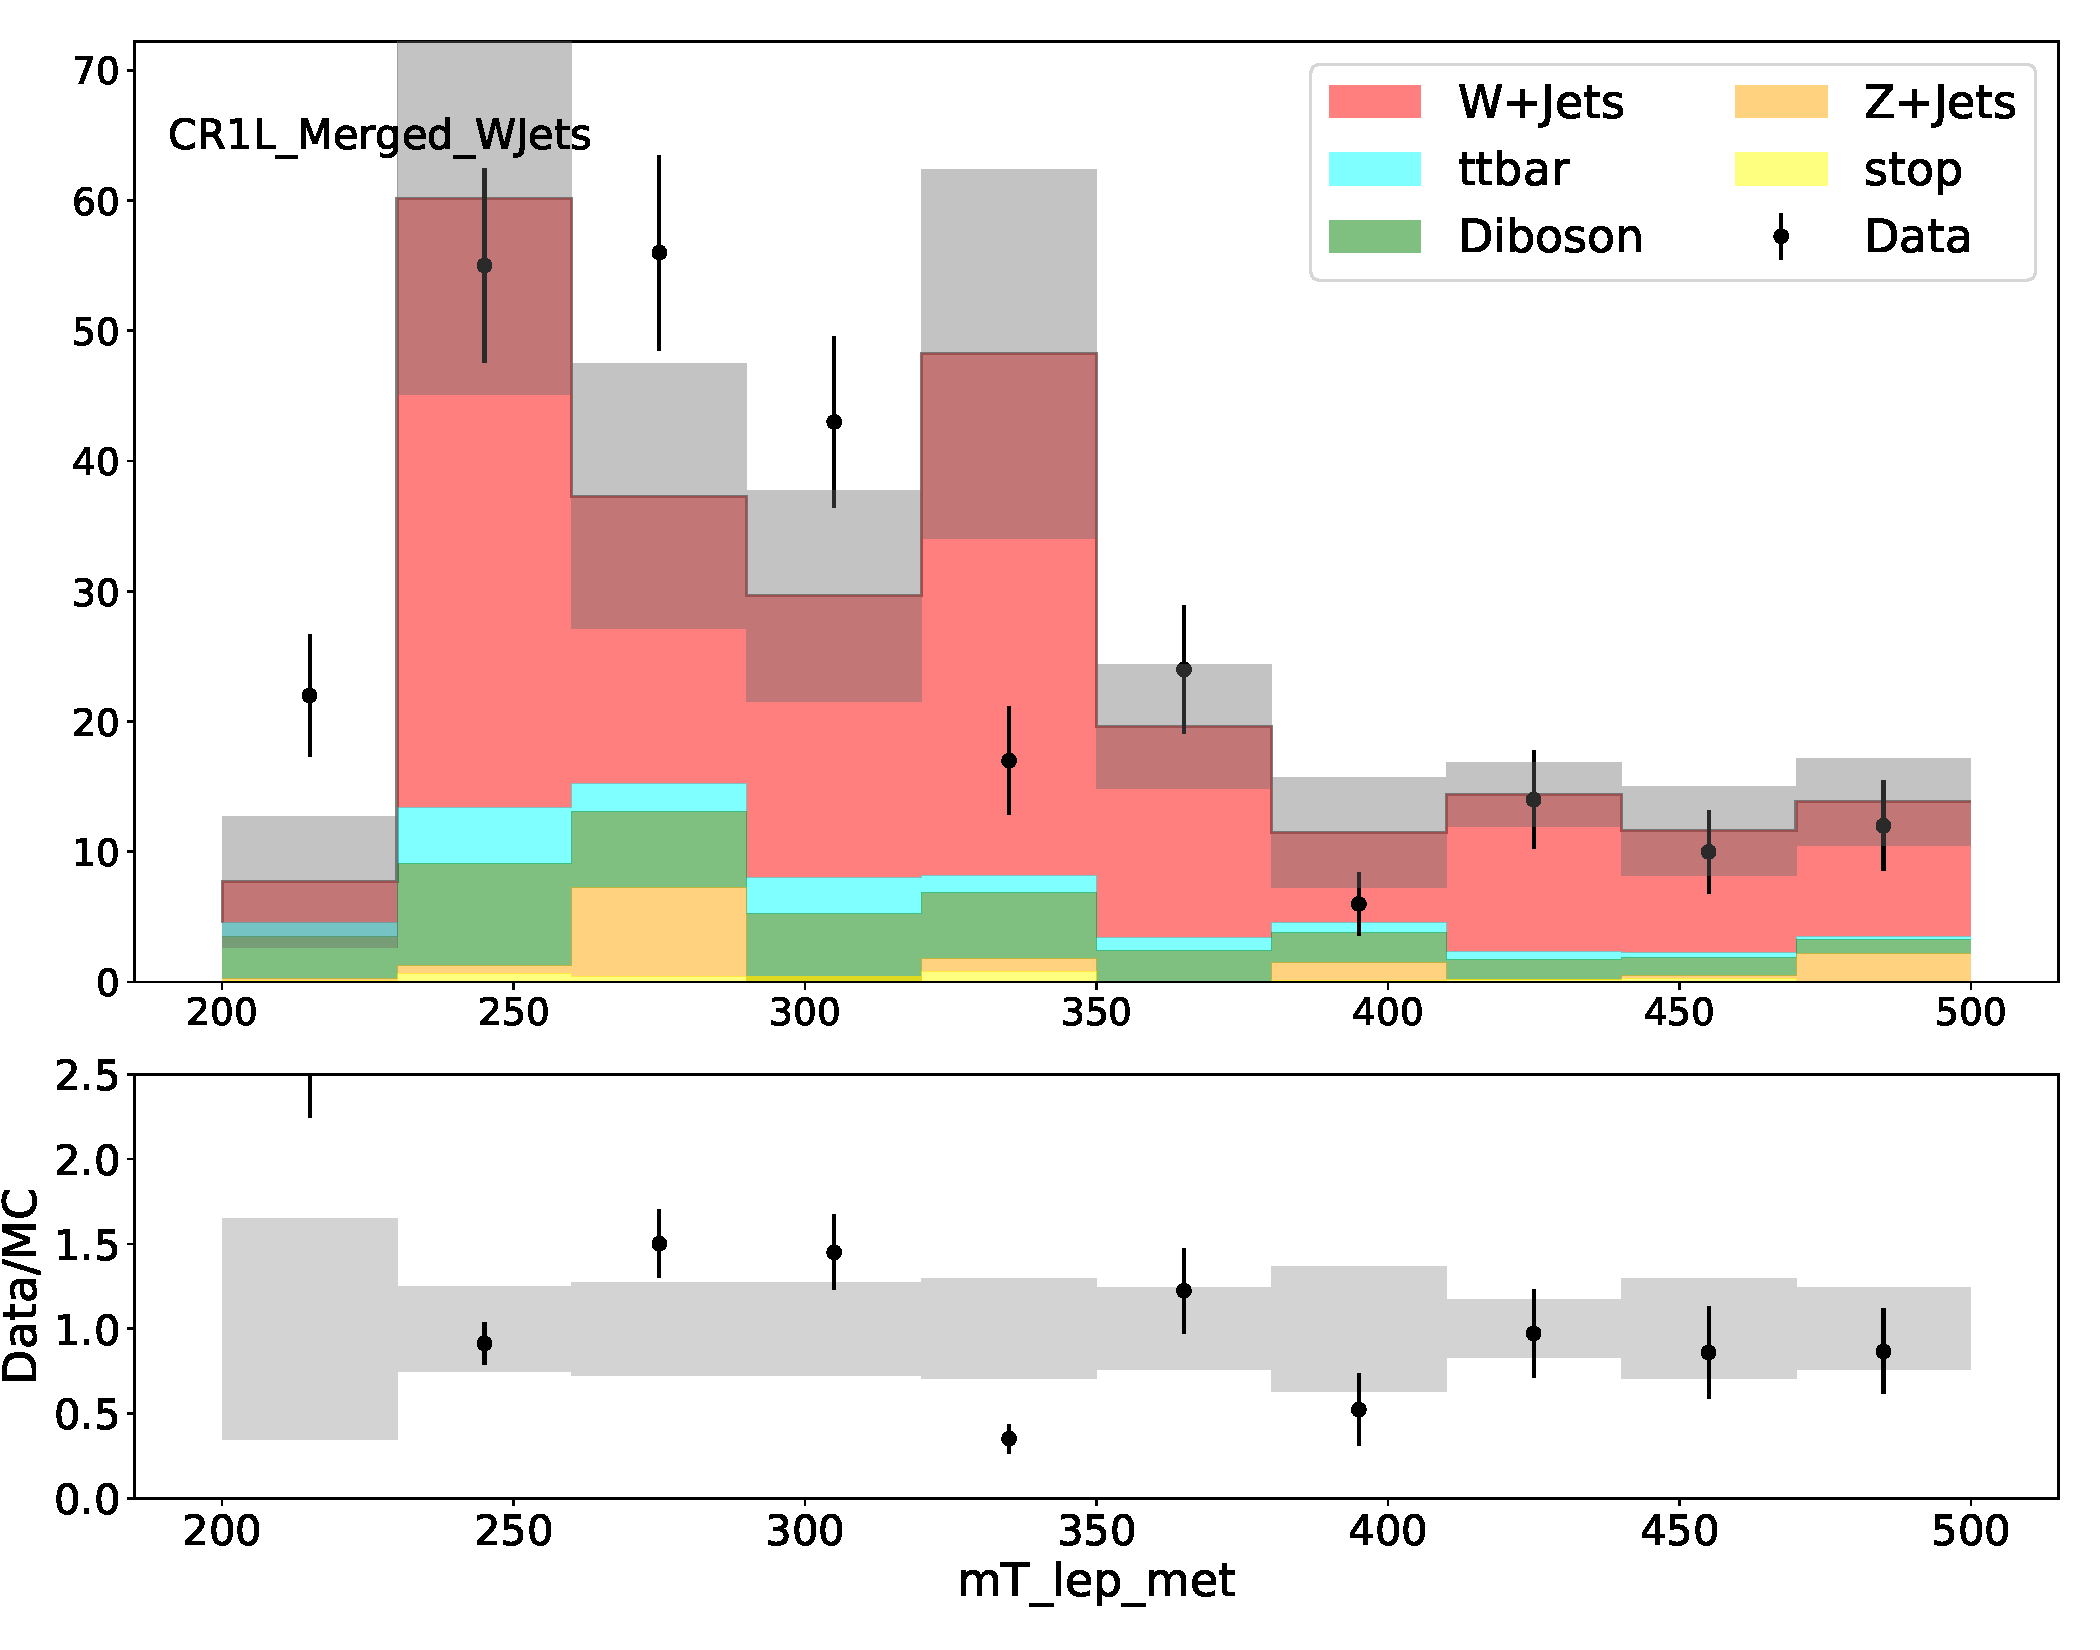
\includegraphics[width = 0.98\textwidth]{Figures/4/datamc/CR1L_Merged_WJets/mT_lep_met.pdf}
    \caption{\mtlepmet}
     \end{subfigure}
    \begin{subfigure}{0.49\textwidth}
     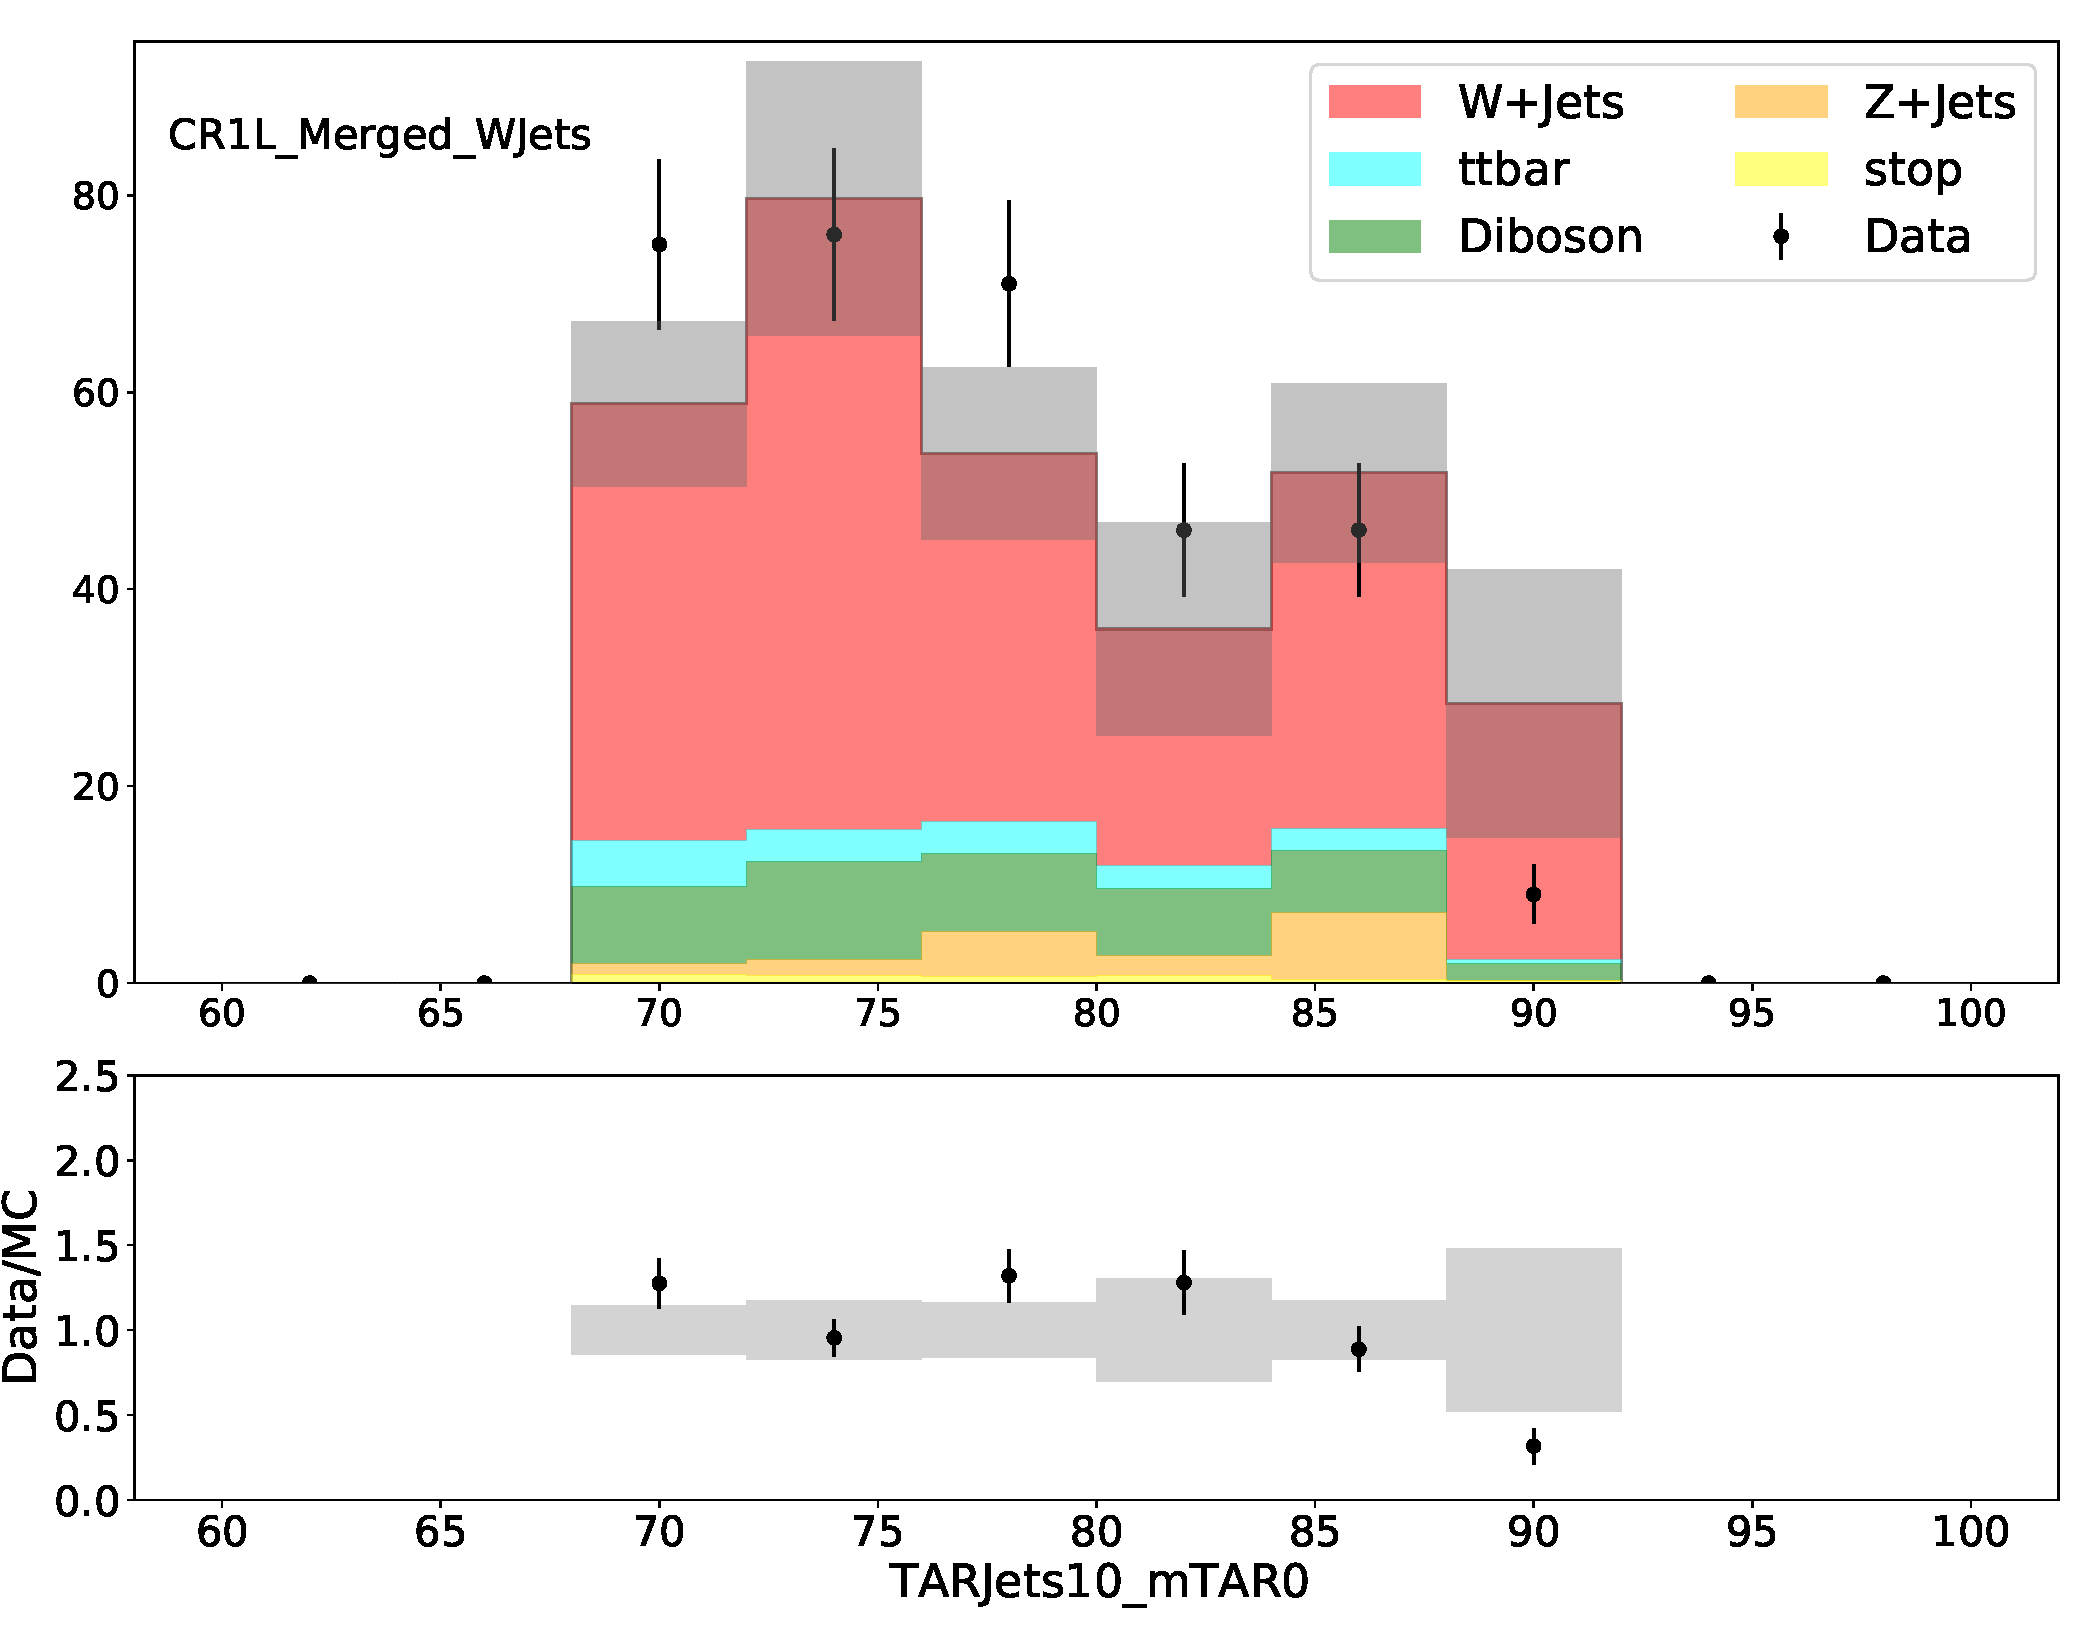
\includegraphics[width = 0.98\textwidth]{Figures/4/datamc/CR1L_Merged_WJets/TARJets10_mTAR0.pdf}
     \caption{\mTAR}
     \end{subfigure}
    \begin{subfigure}{0.49\textwidth}
     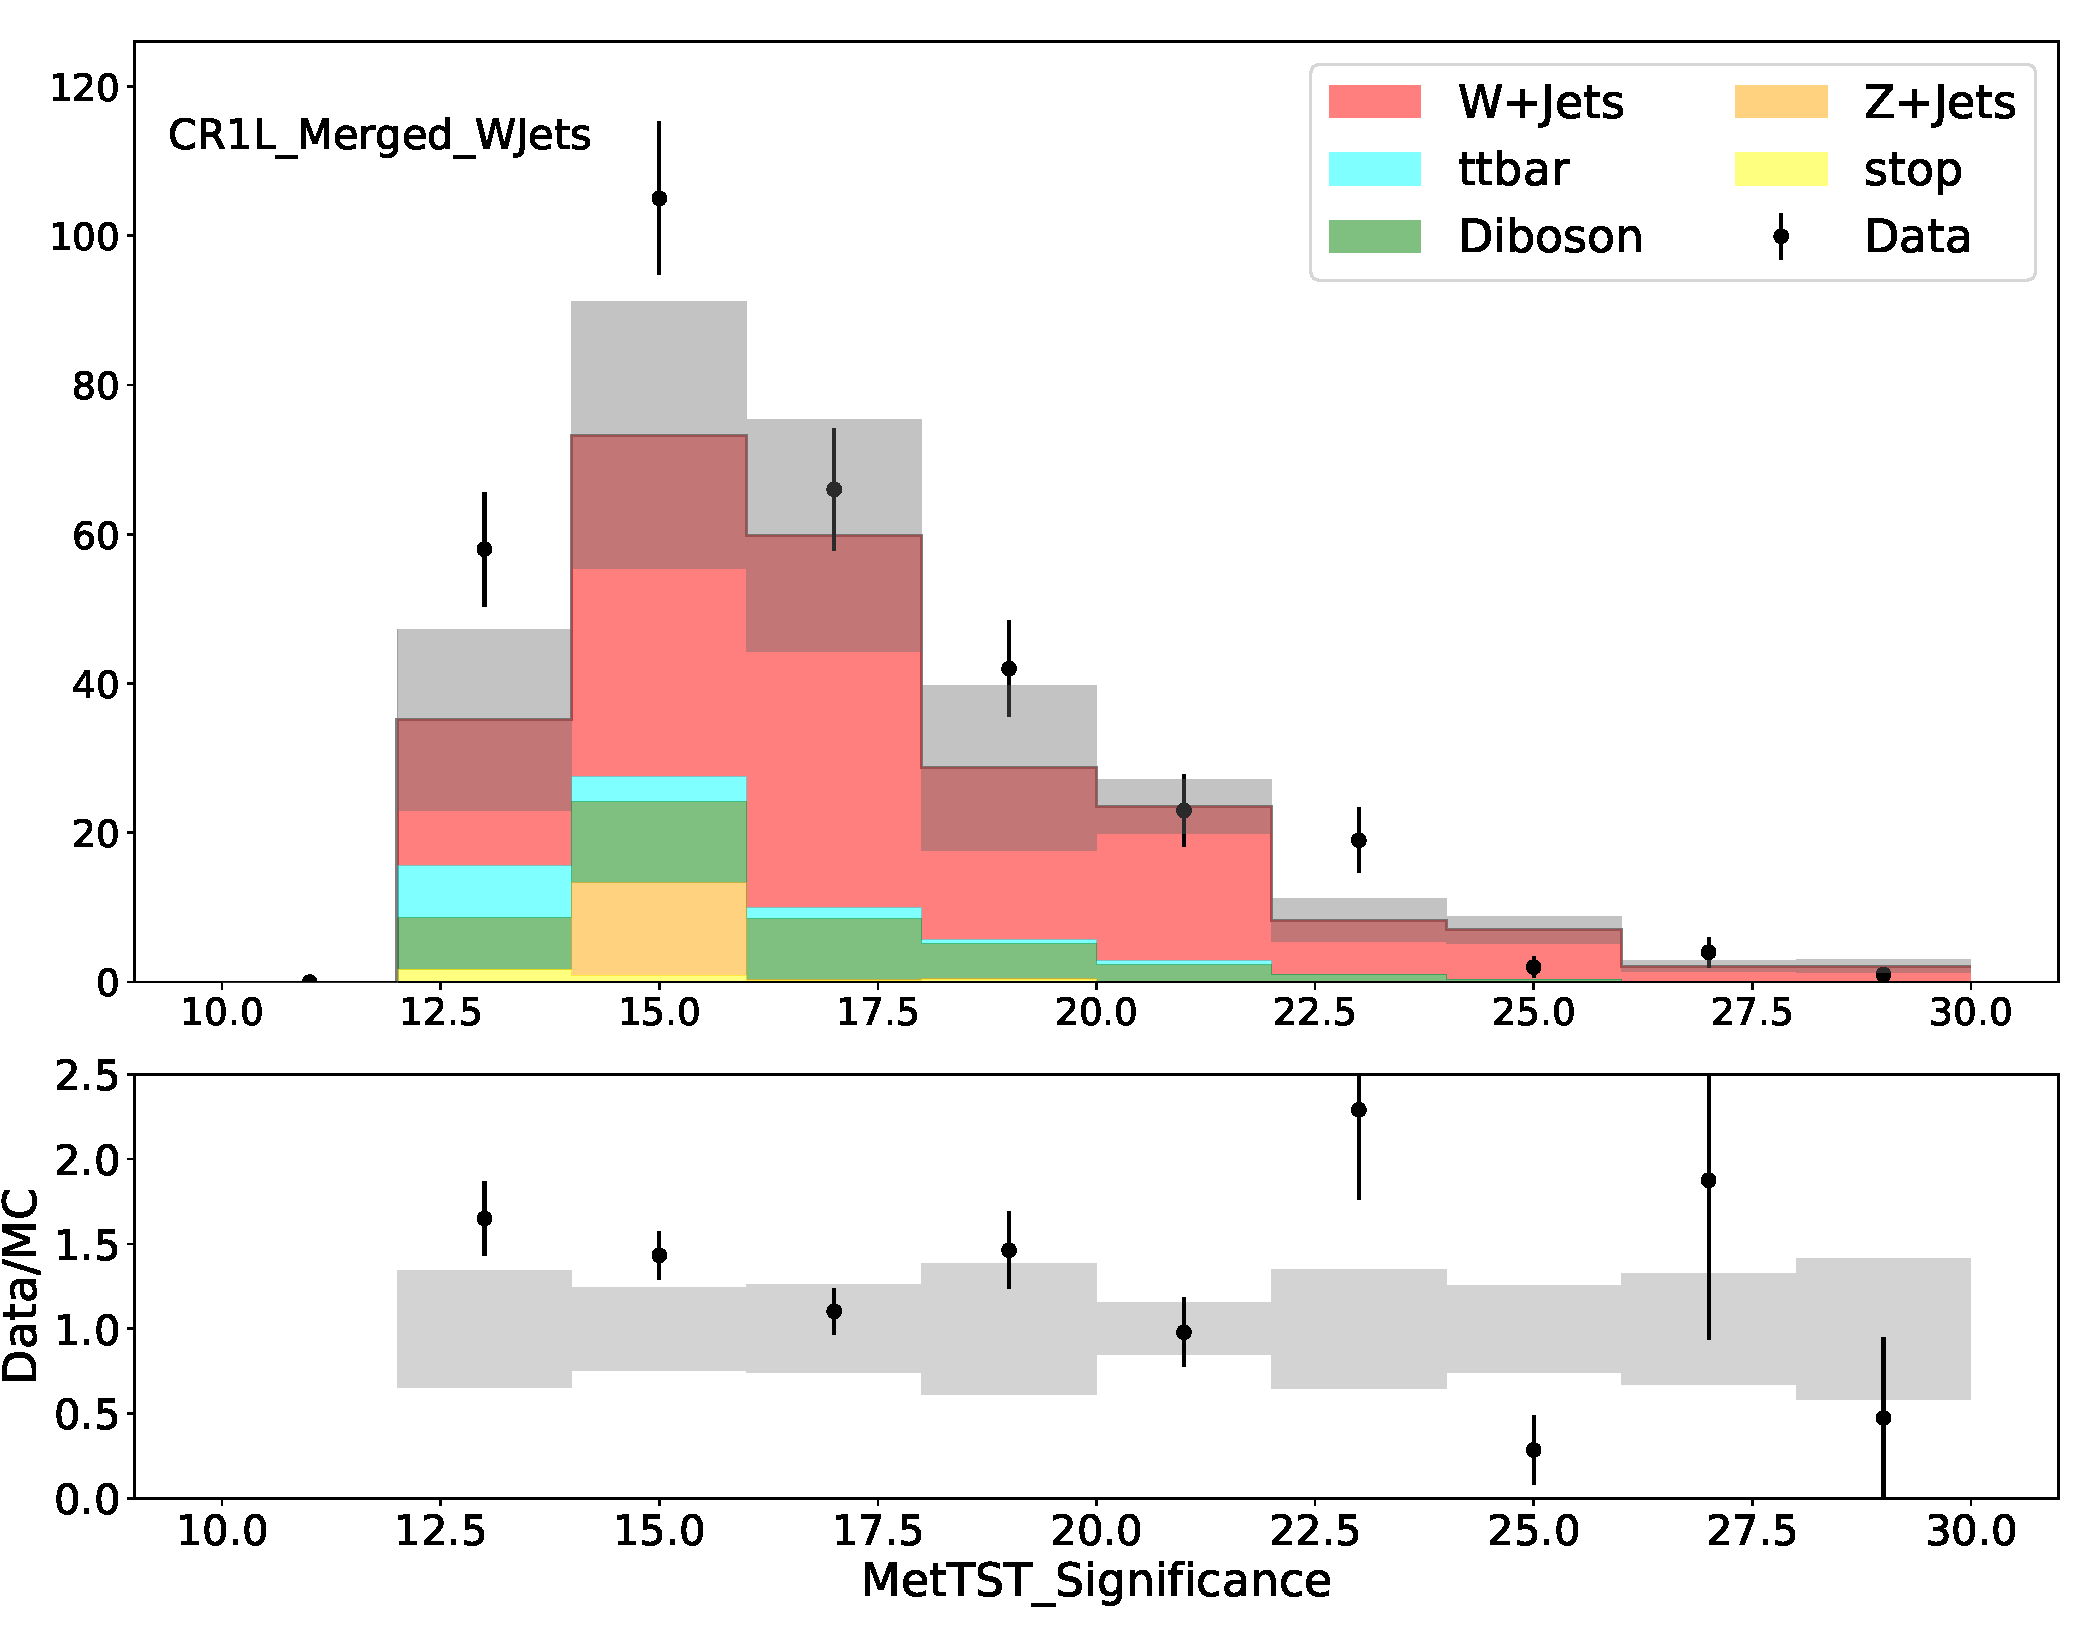
\includegraphics[width = 0.98\textwidth]{Figures/4/datamc/CR1L_Merged_WJets/MetTST_Significance.pdf}
     \caption{\metsig}
     \end{subfigure}
    \begin{subfigure}{0.49\textwidth}
     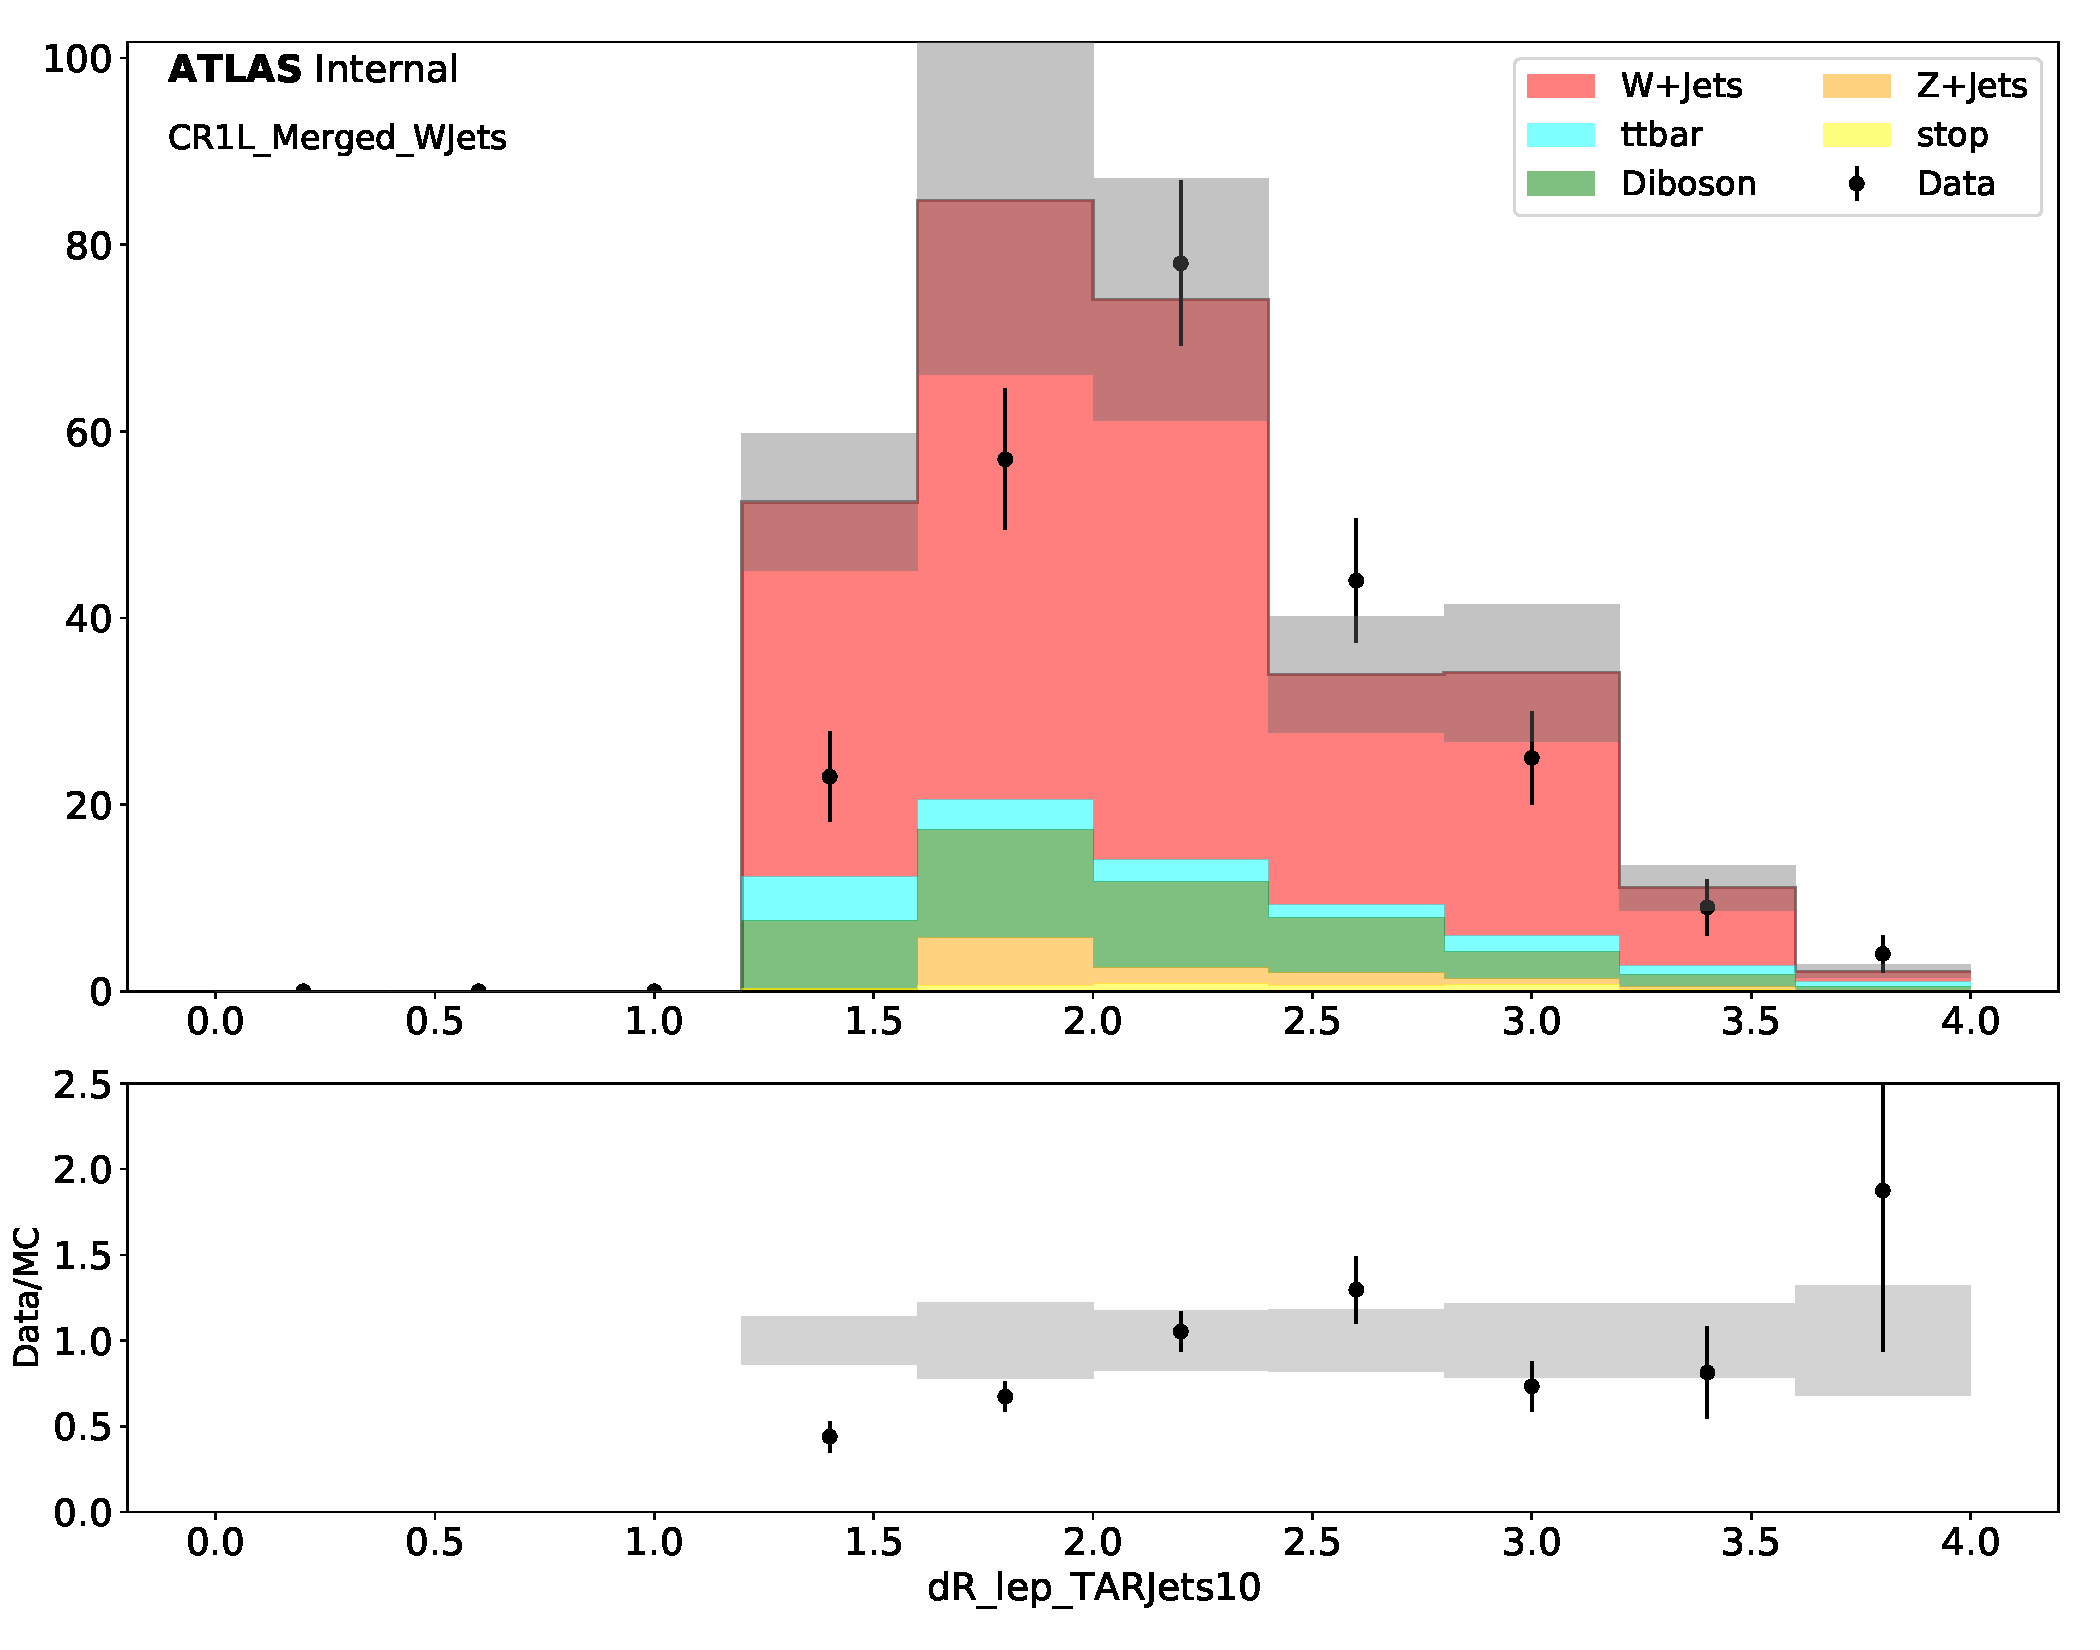
\includegraphics[width = 0.98\textwidth]{Figures/4/datamc/CR1L_Merged_WJets/dR_lep_TARJets10.pdf}
     \caption{\drTARl}
     \end{subfigure}
     \caption{Data-MC comparisons in the \merged \wjets control region. Grey bands represent MC statistical uncertainty on each bin.}
     \label{fig:Data_MC_CRdR_merged}
  \end{figure}

\begin{figure}[htbp]
  \centering
     \begin{subfigure}{0.49\textwidth}
     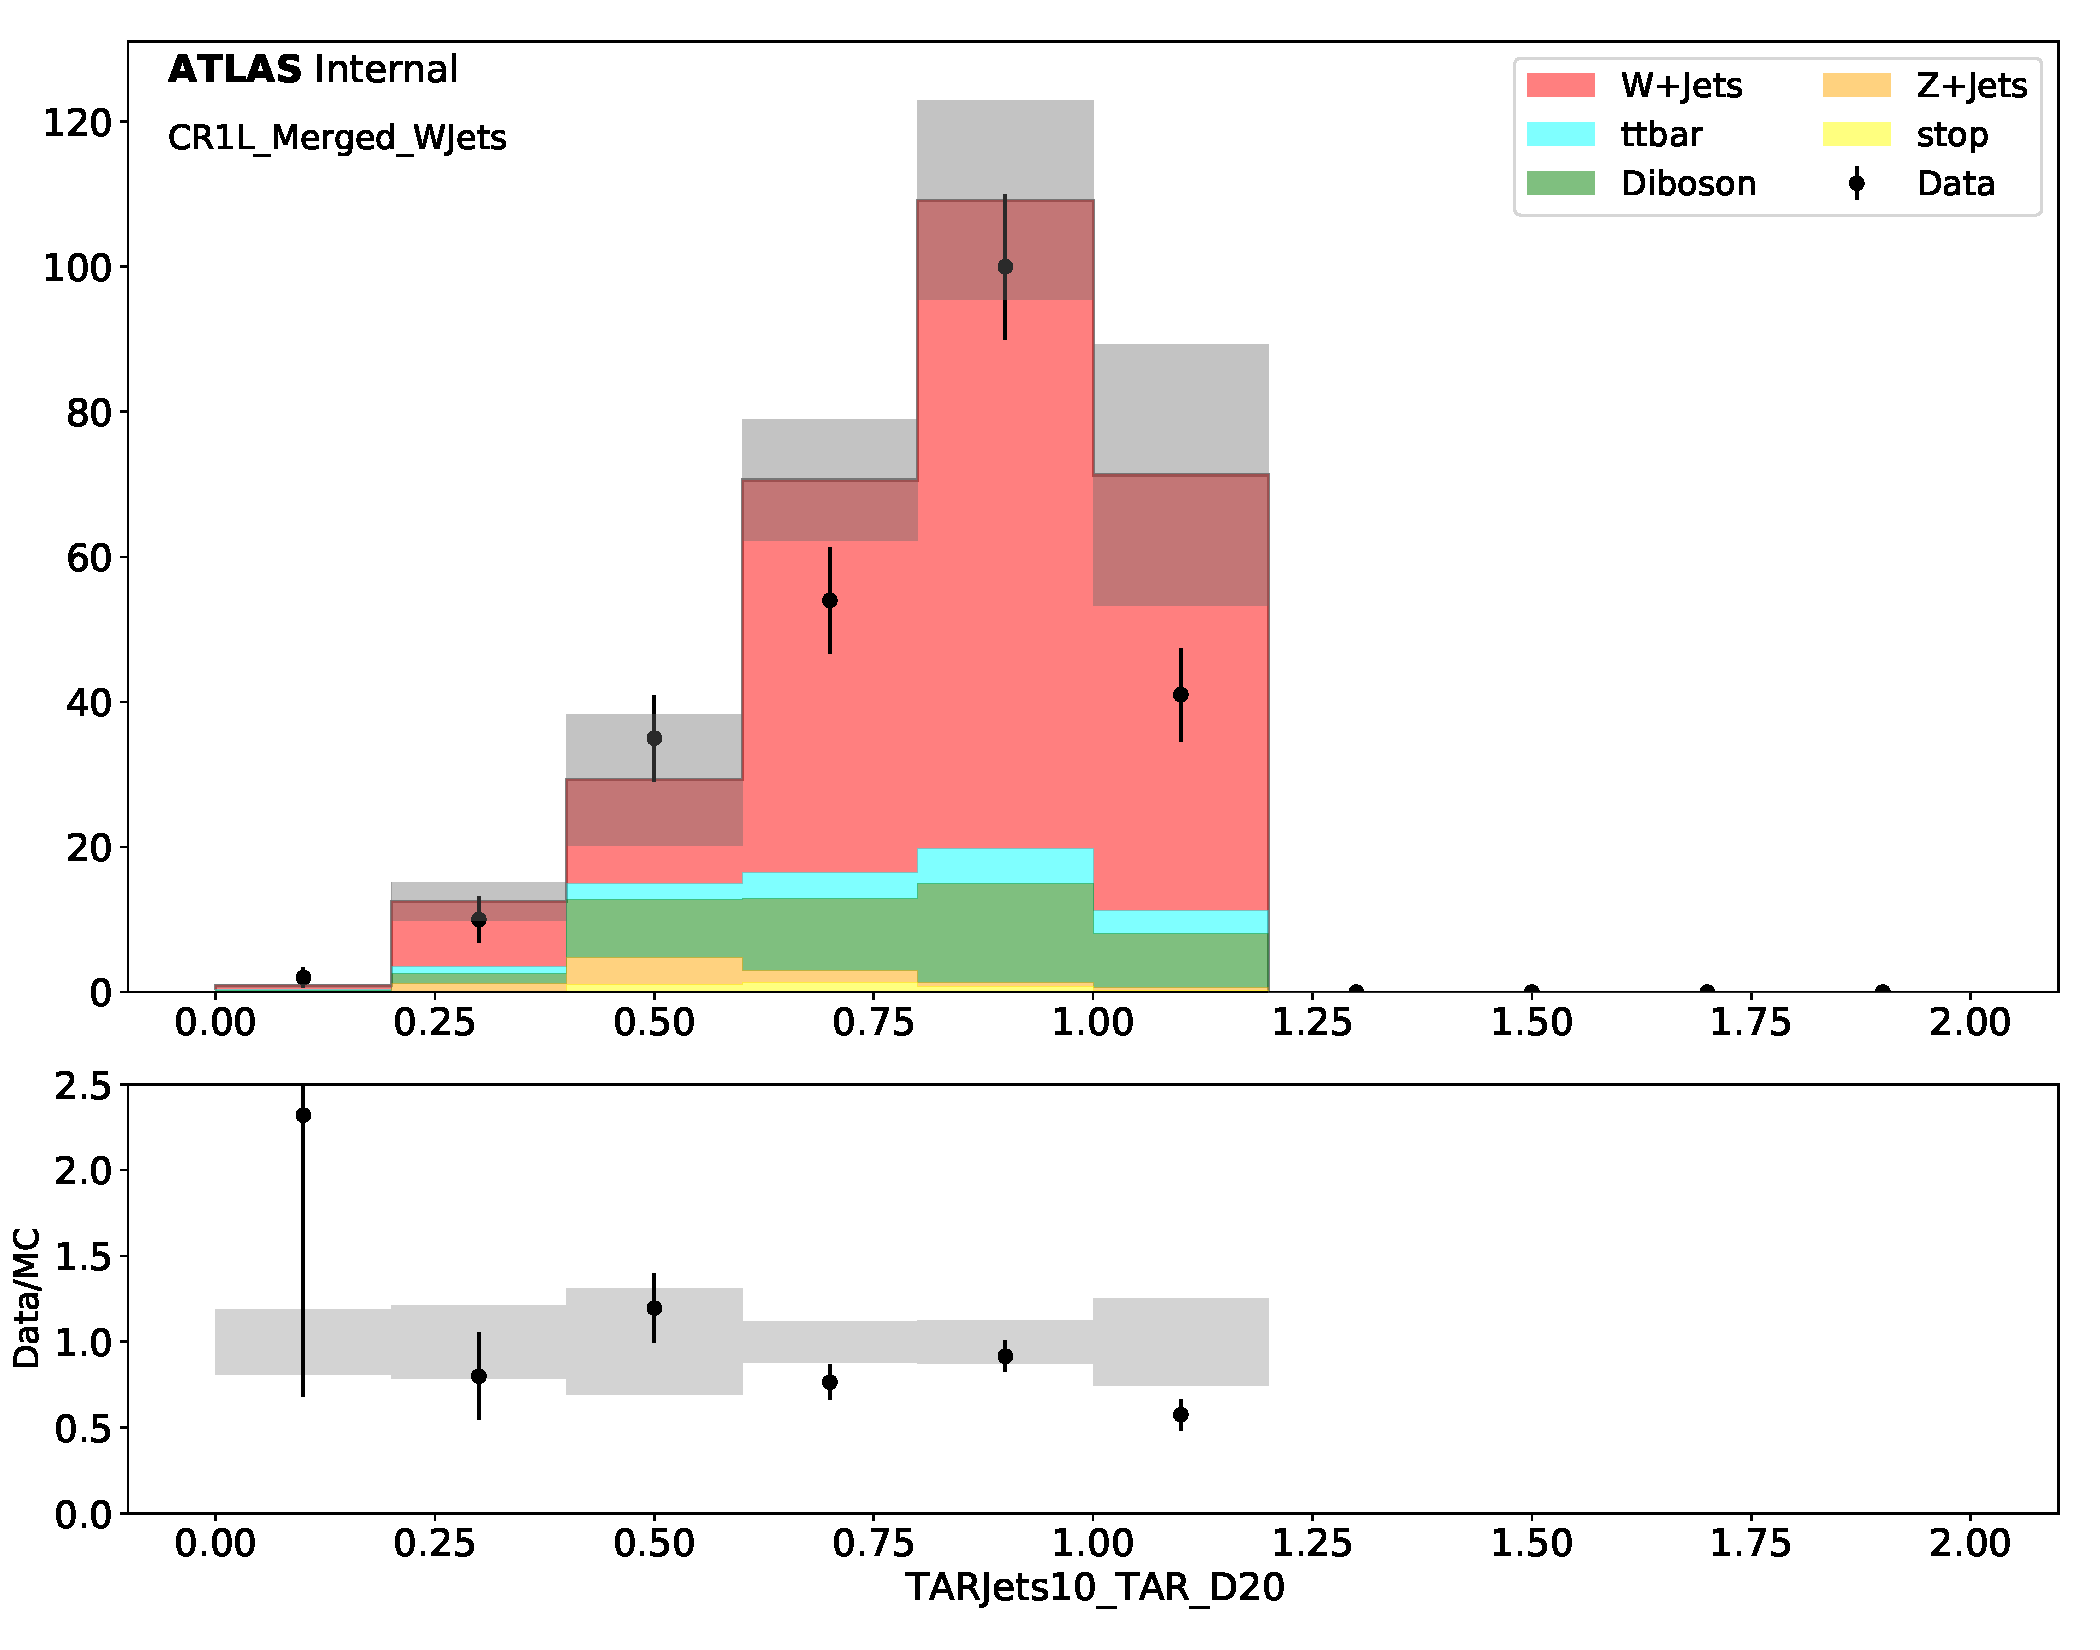
\includegraphics[width = 0.98\textwidth]{Figures/4/datamc/CR1L_Merged_WJets/TARJets10_TAR_D20.pdf}
     \caption{\DtwoTAR}
     \end{subfigure}
     \begin{subfigure}{0.49\textwidth}
     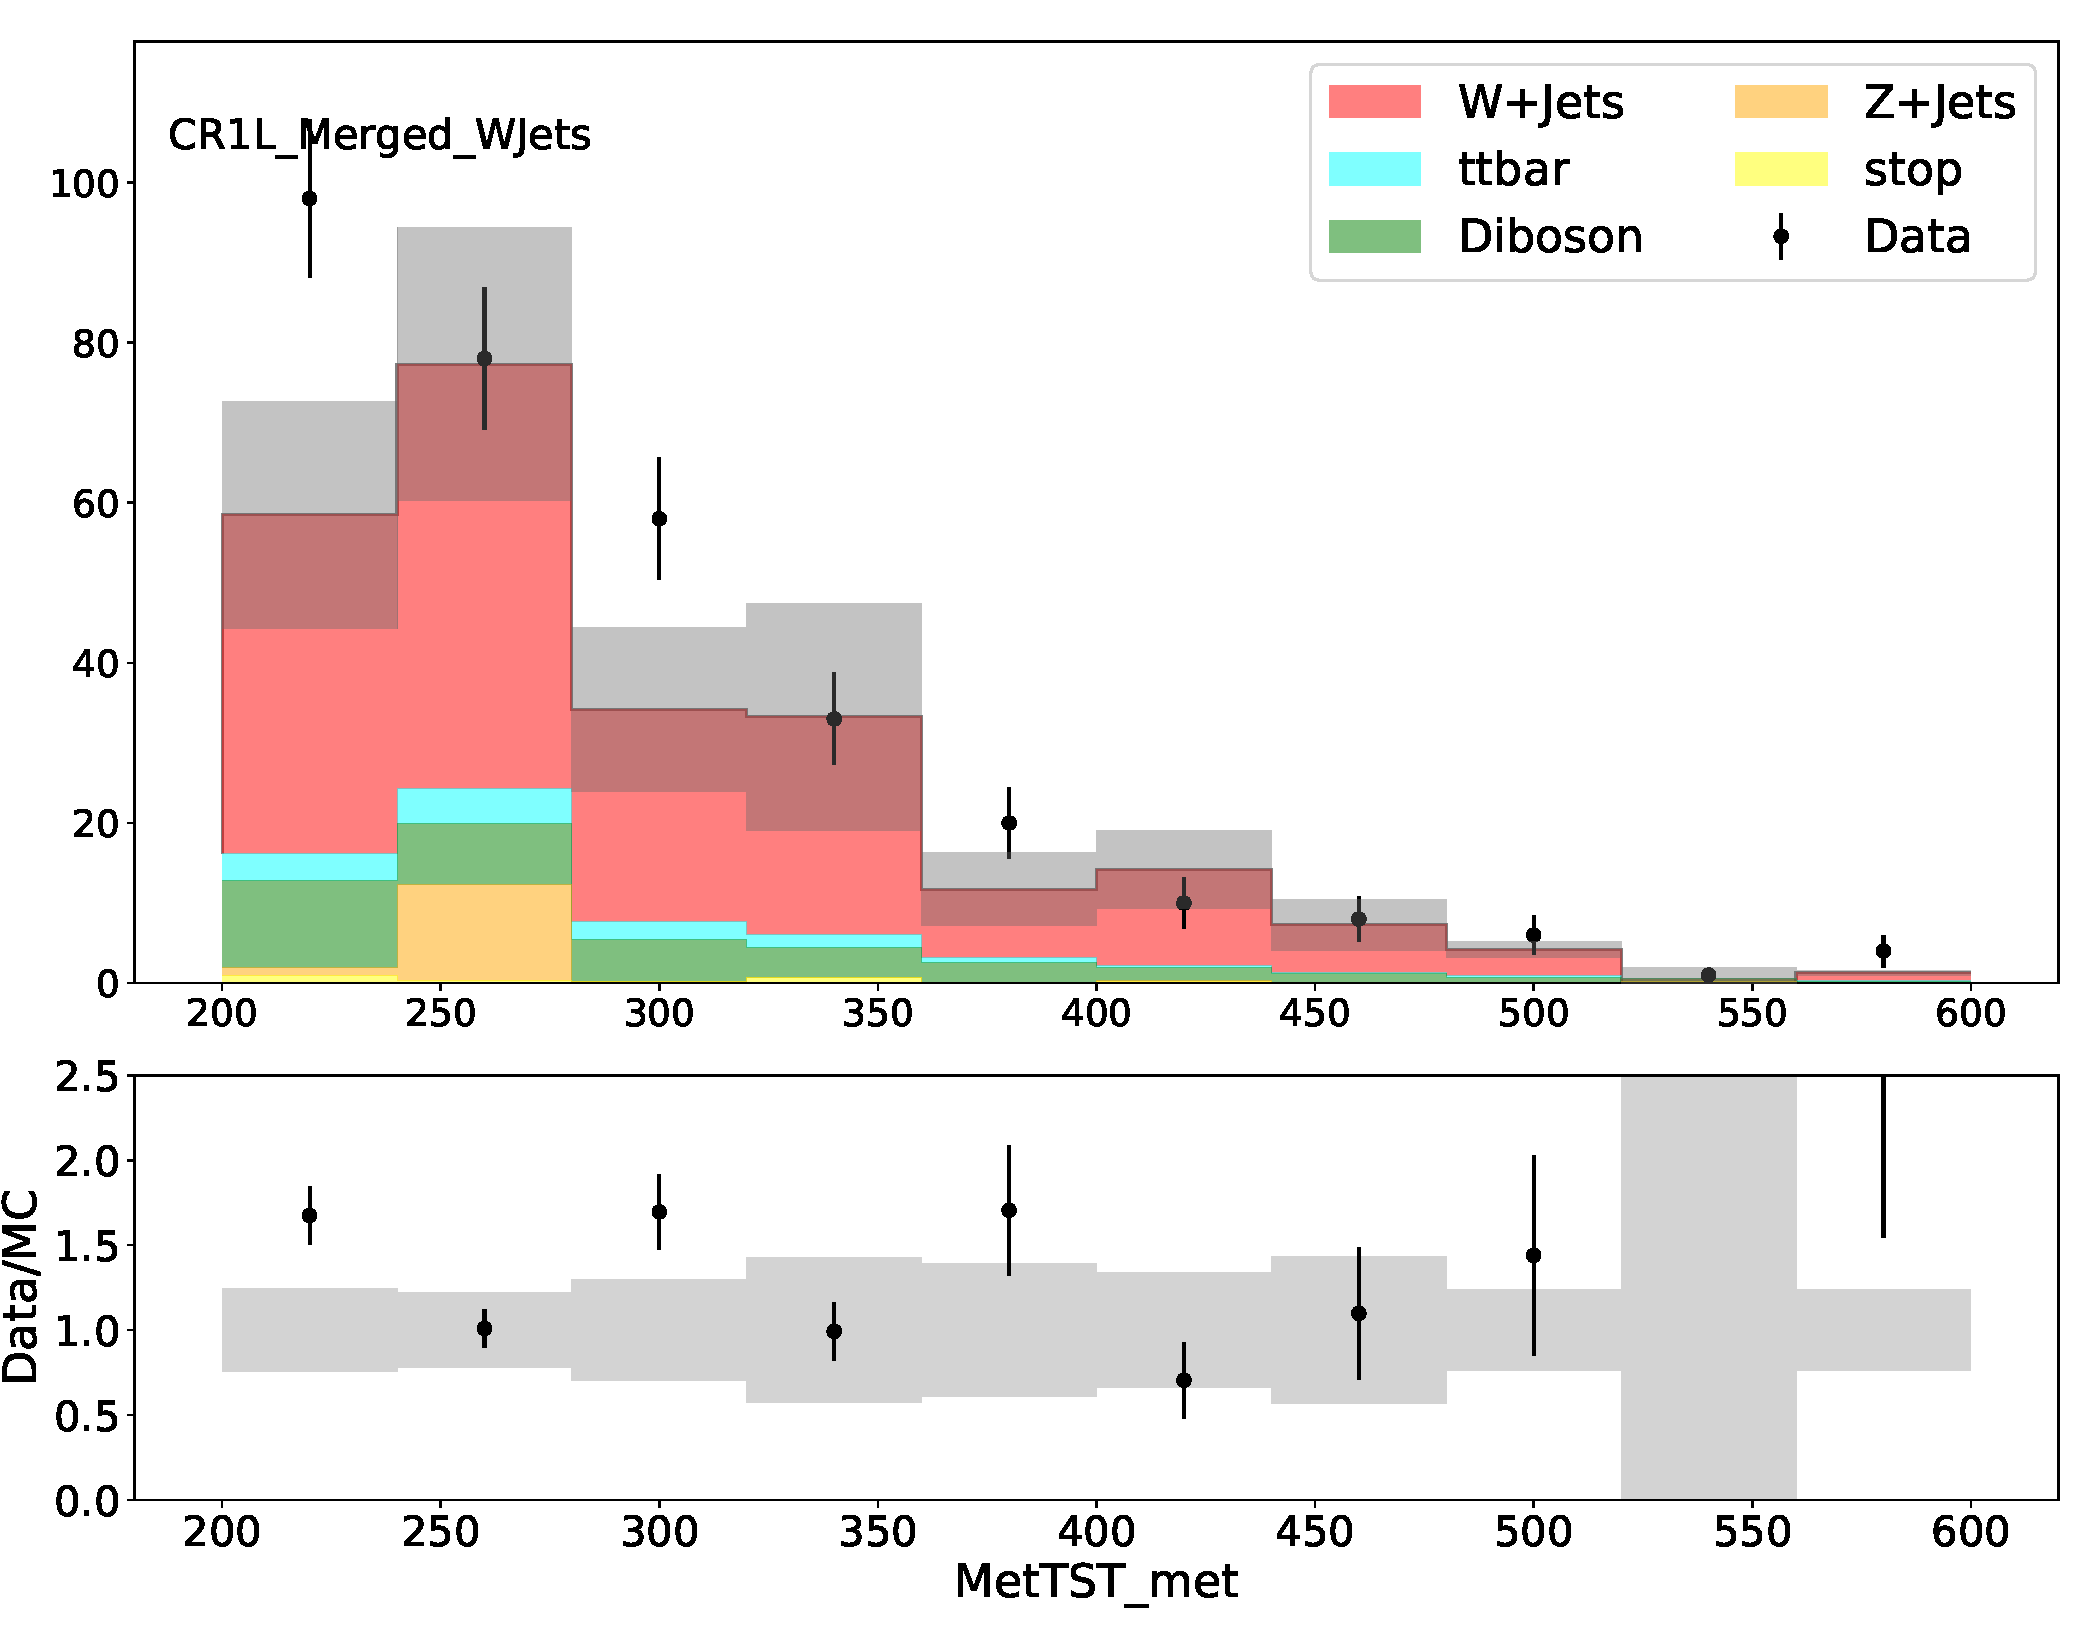
\includegraphics[width = 0.98\textwidth]{Figures/4/datamc/CR1L_Merged_WJets/MetTST_met.pdf}
     \caption{\met}
     \end{subfigure}

     \caption{Data-MC comparisons in the \merged \wjets control region. Grey bands represent MC statistical uncertainty on each bin.}
     \label{fig:Data_MC_CRdR_merged}
  \end{figure}

\begin{figure}[htbp]
  \centering
     \begin{subfigure}{0.49\textwidth}
     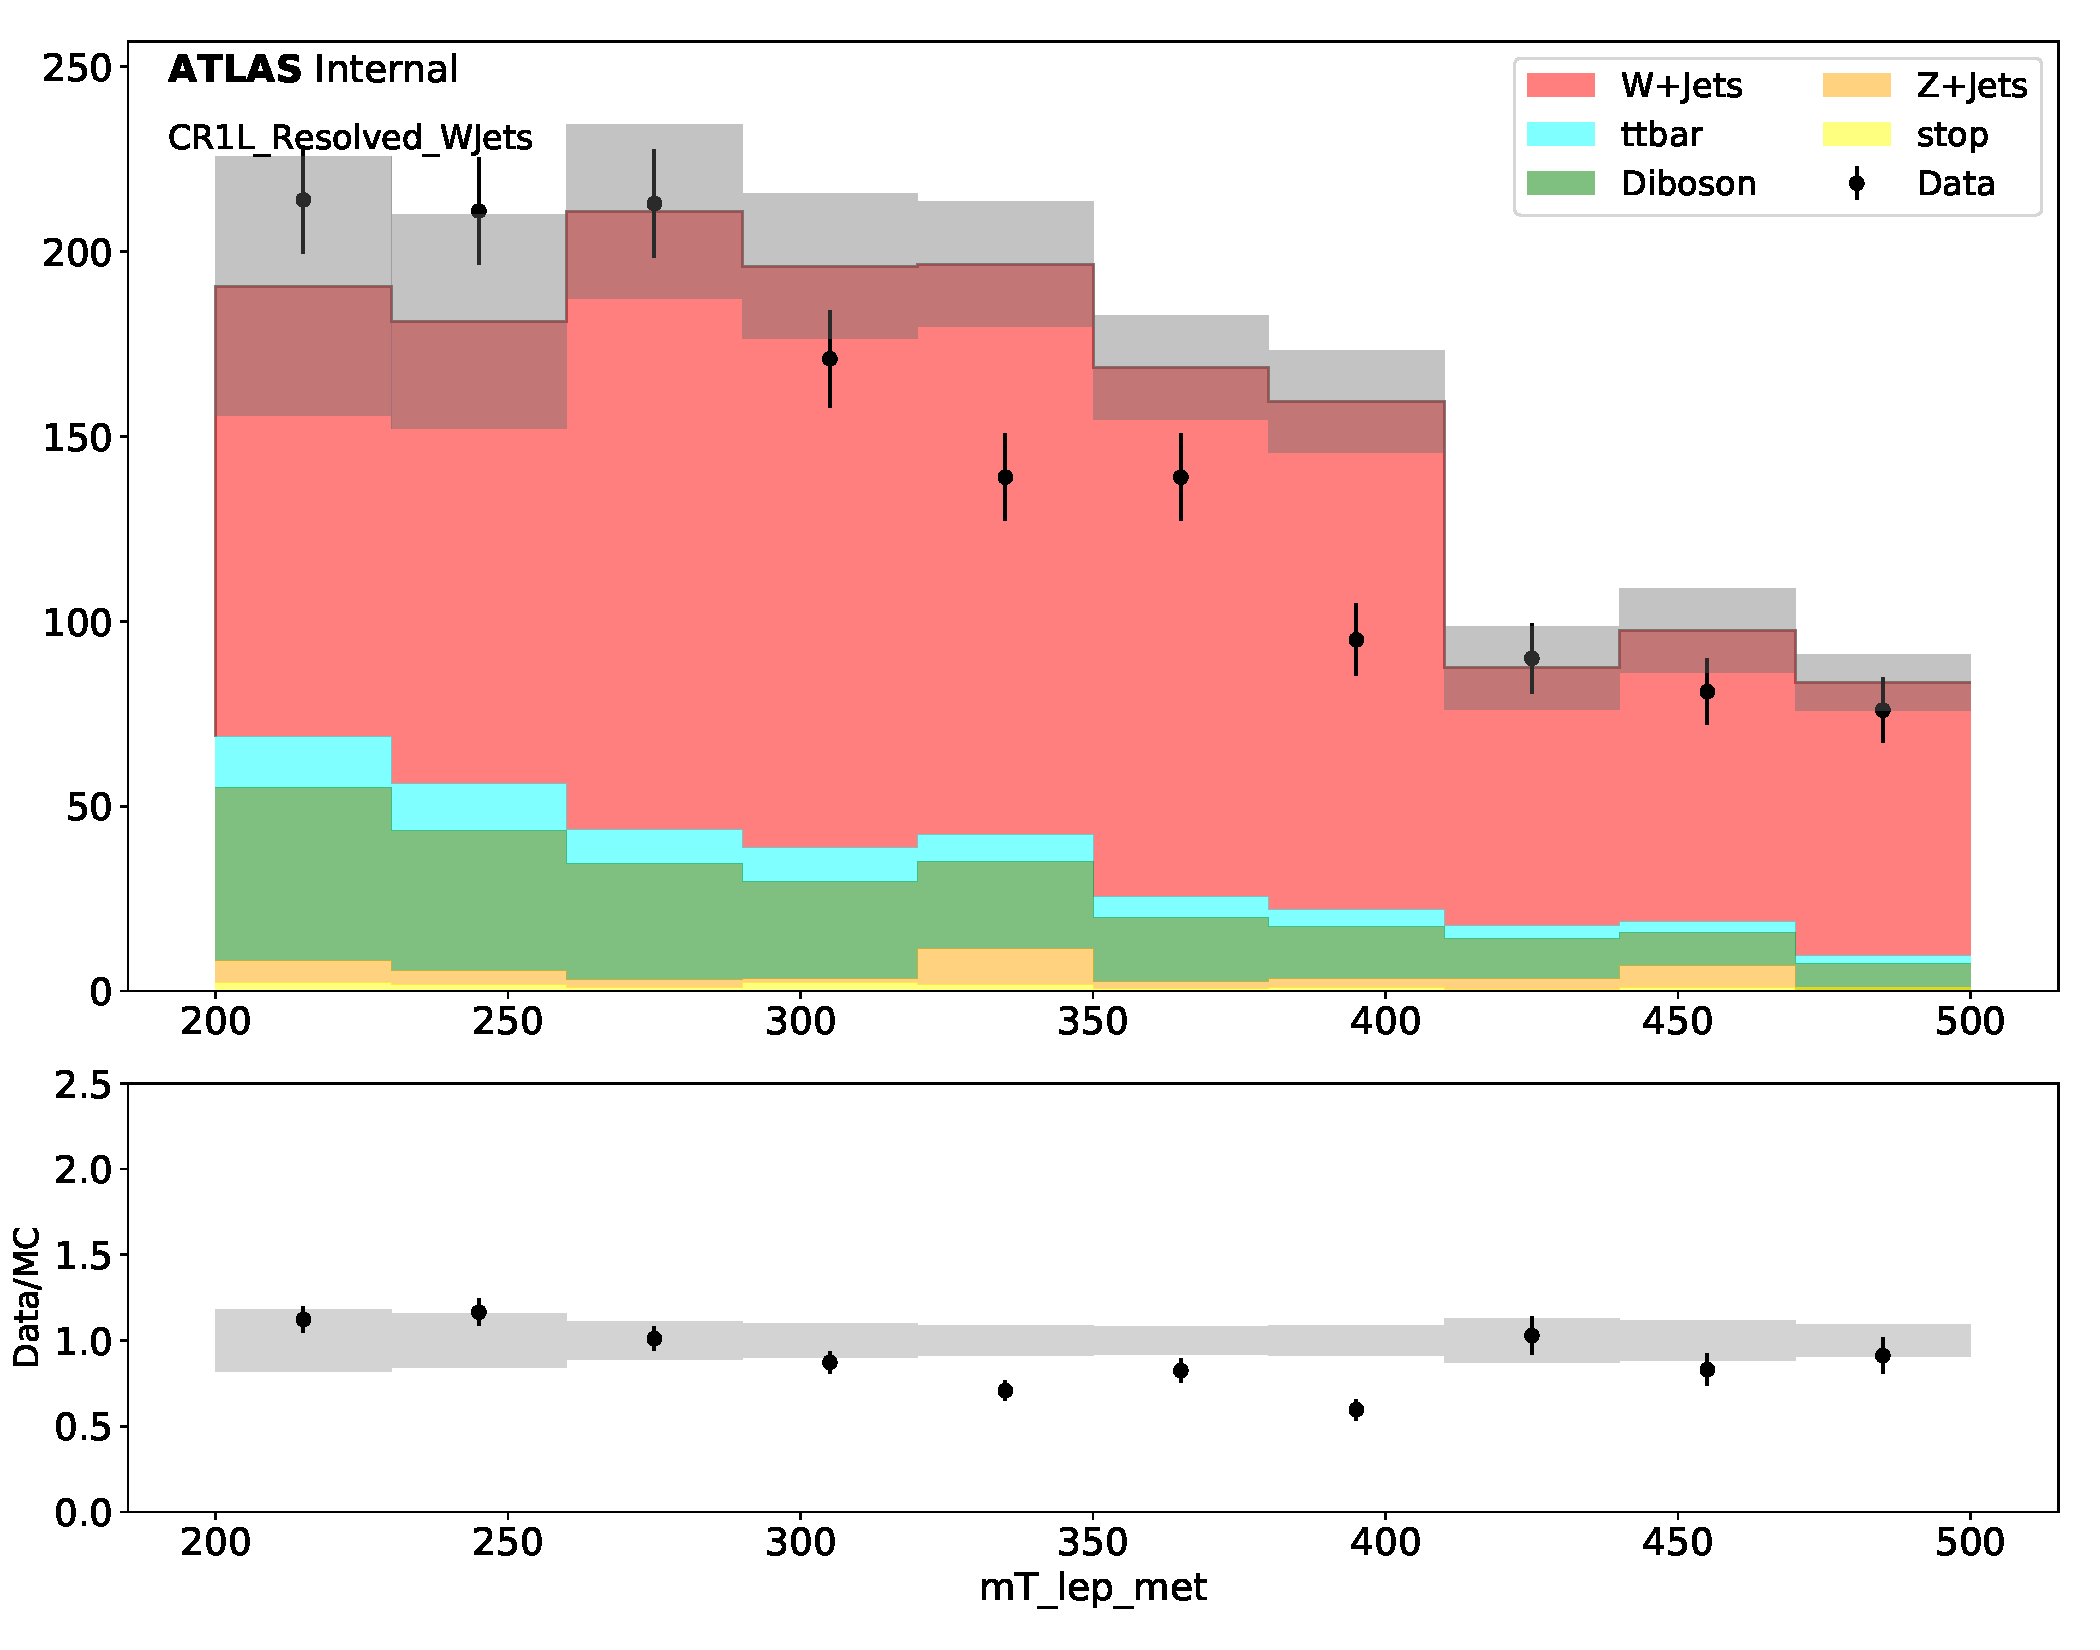
\includegraphics[width = 0.98\textwidth]{Figures/4/datamc/CR1L_Resolved_WJets/mT_lep_met.pdf}
     \caption{\mtlepmet}
     \end{subfigure}
     \begin{subfigure}{0.49\textwidth}
     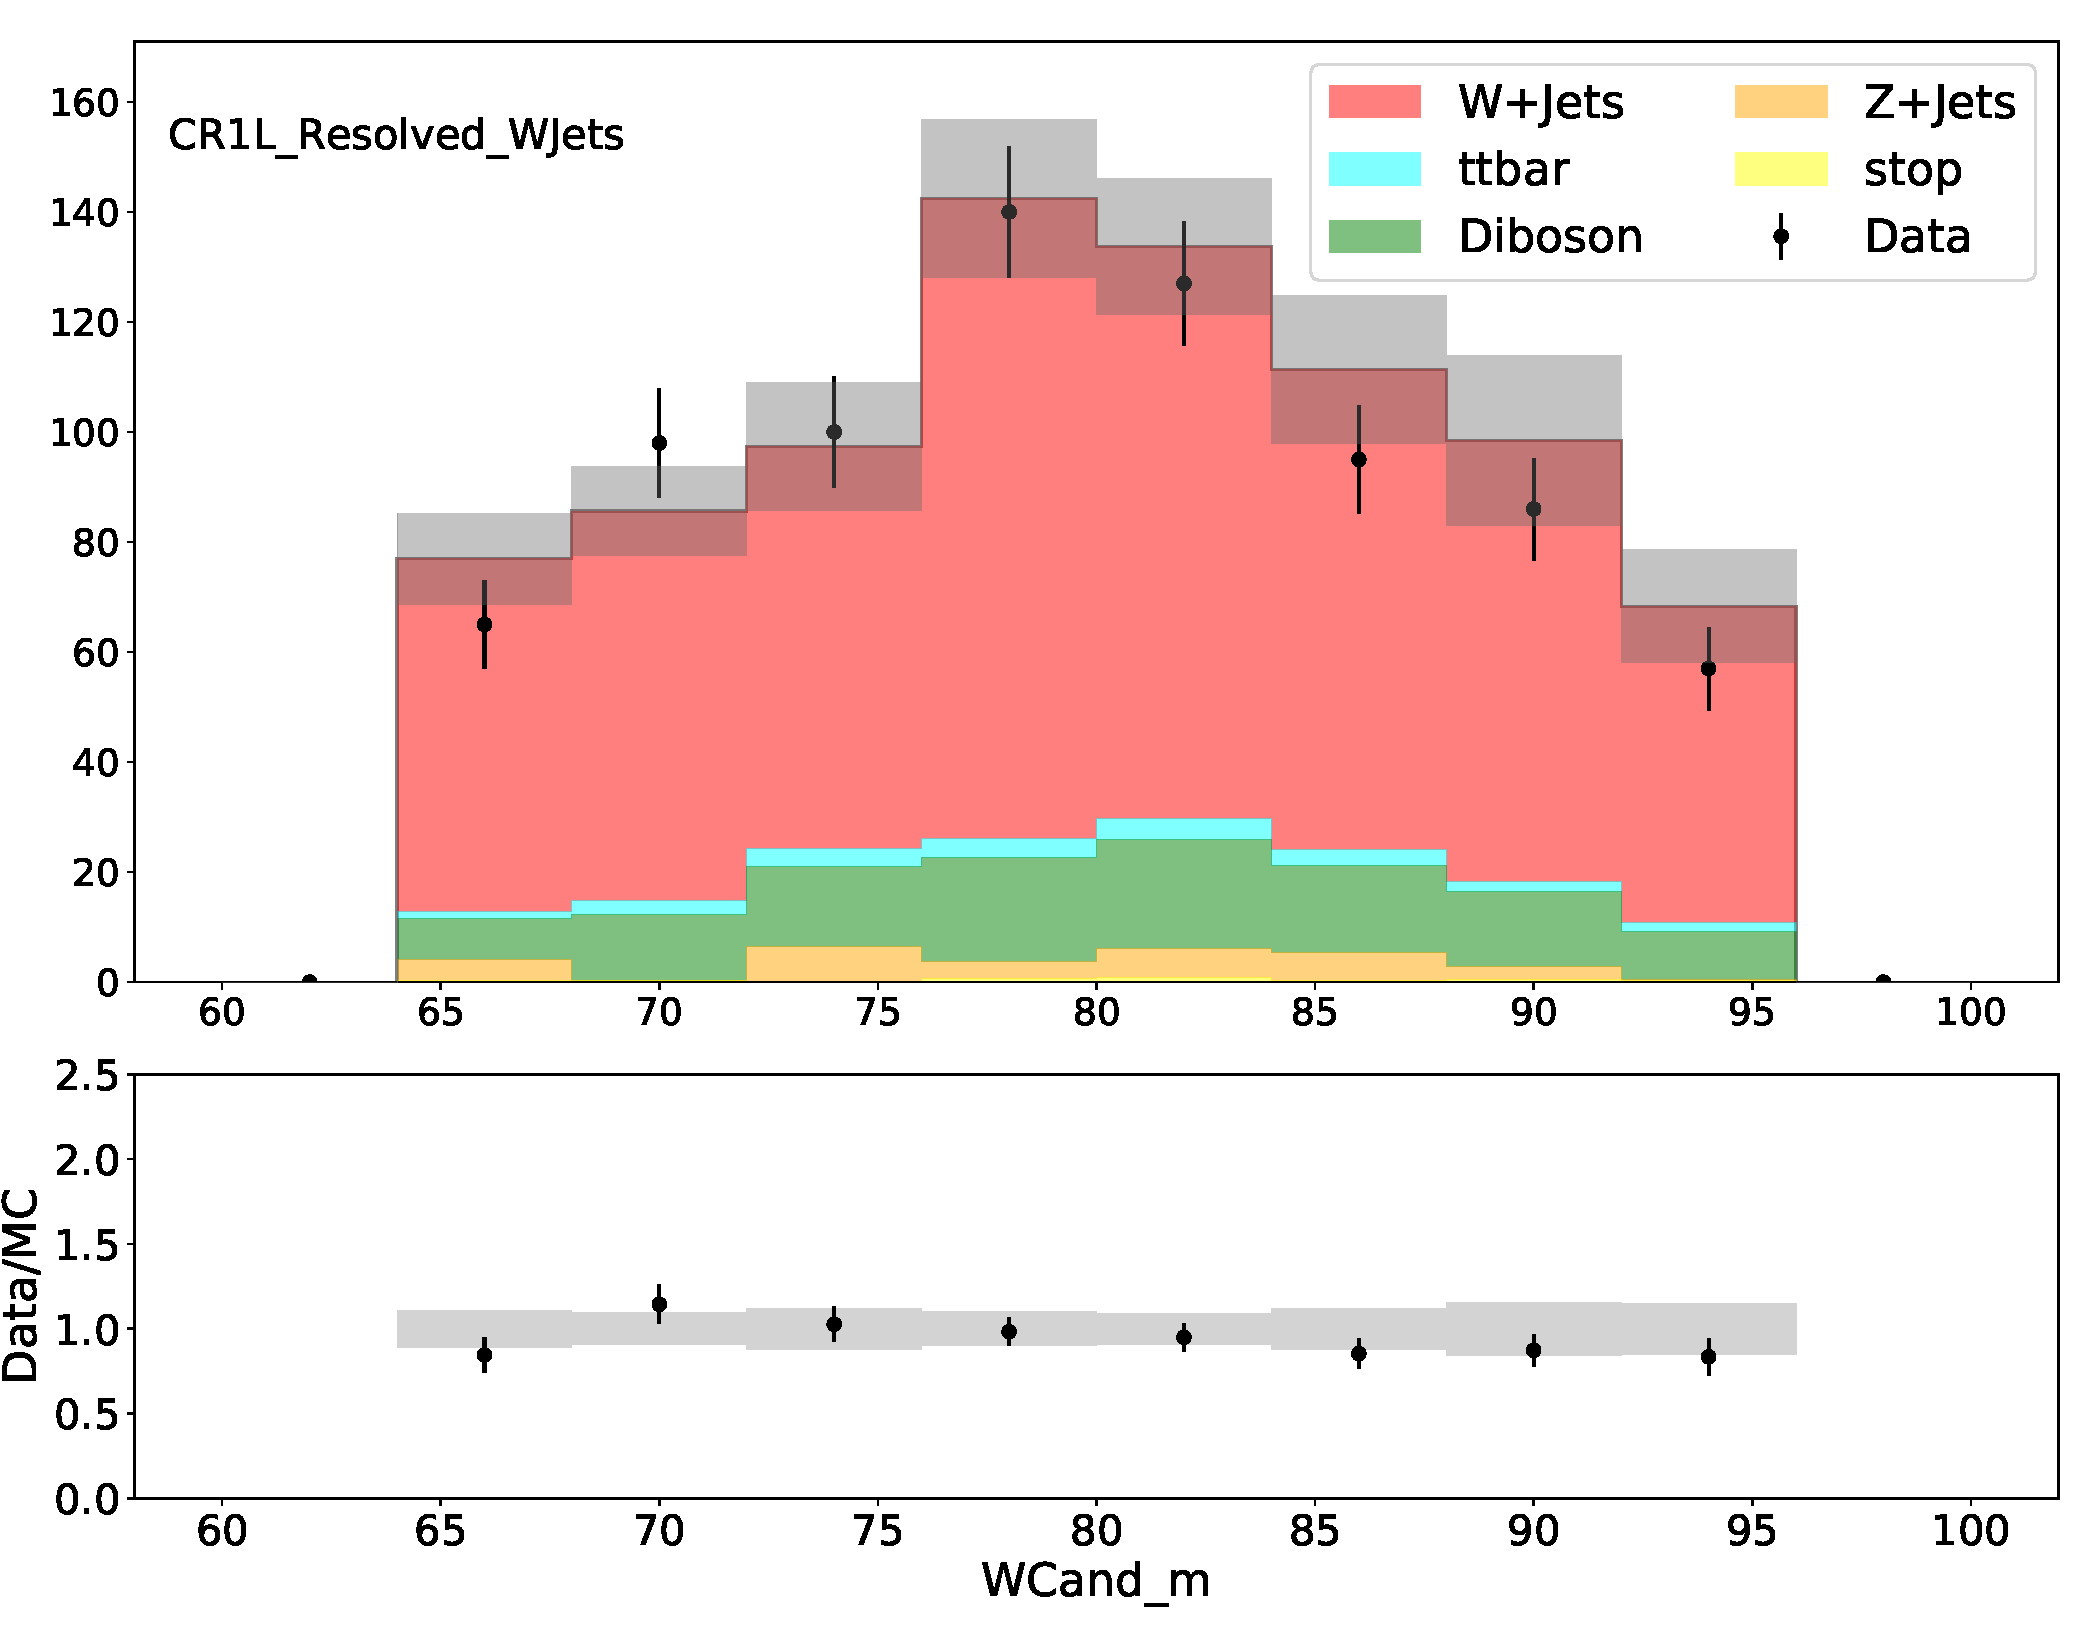
\includegraphics[width = 0.98\textwidth]{Figures/4/datamc/CR1L_Resolved_WJets/WCand_m.pdf}
     \caption{\Wcandm}
     \end{subfigure}
     \begin{subfigure}{0.49\textwidth}
     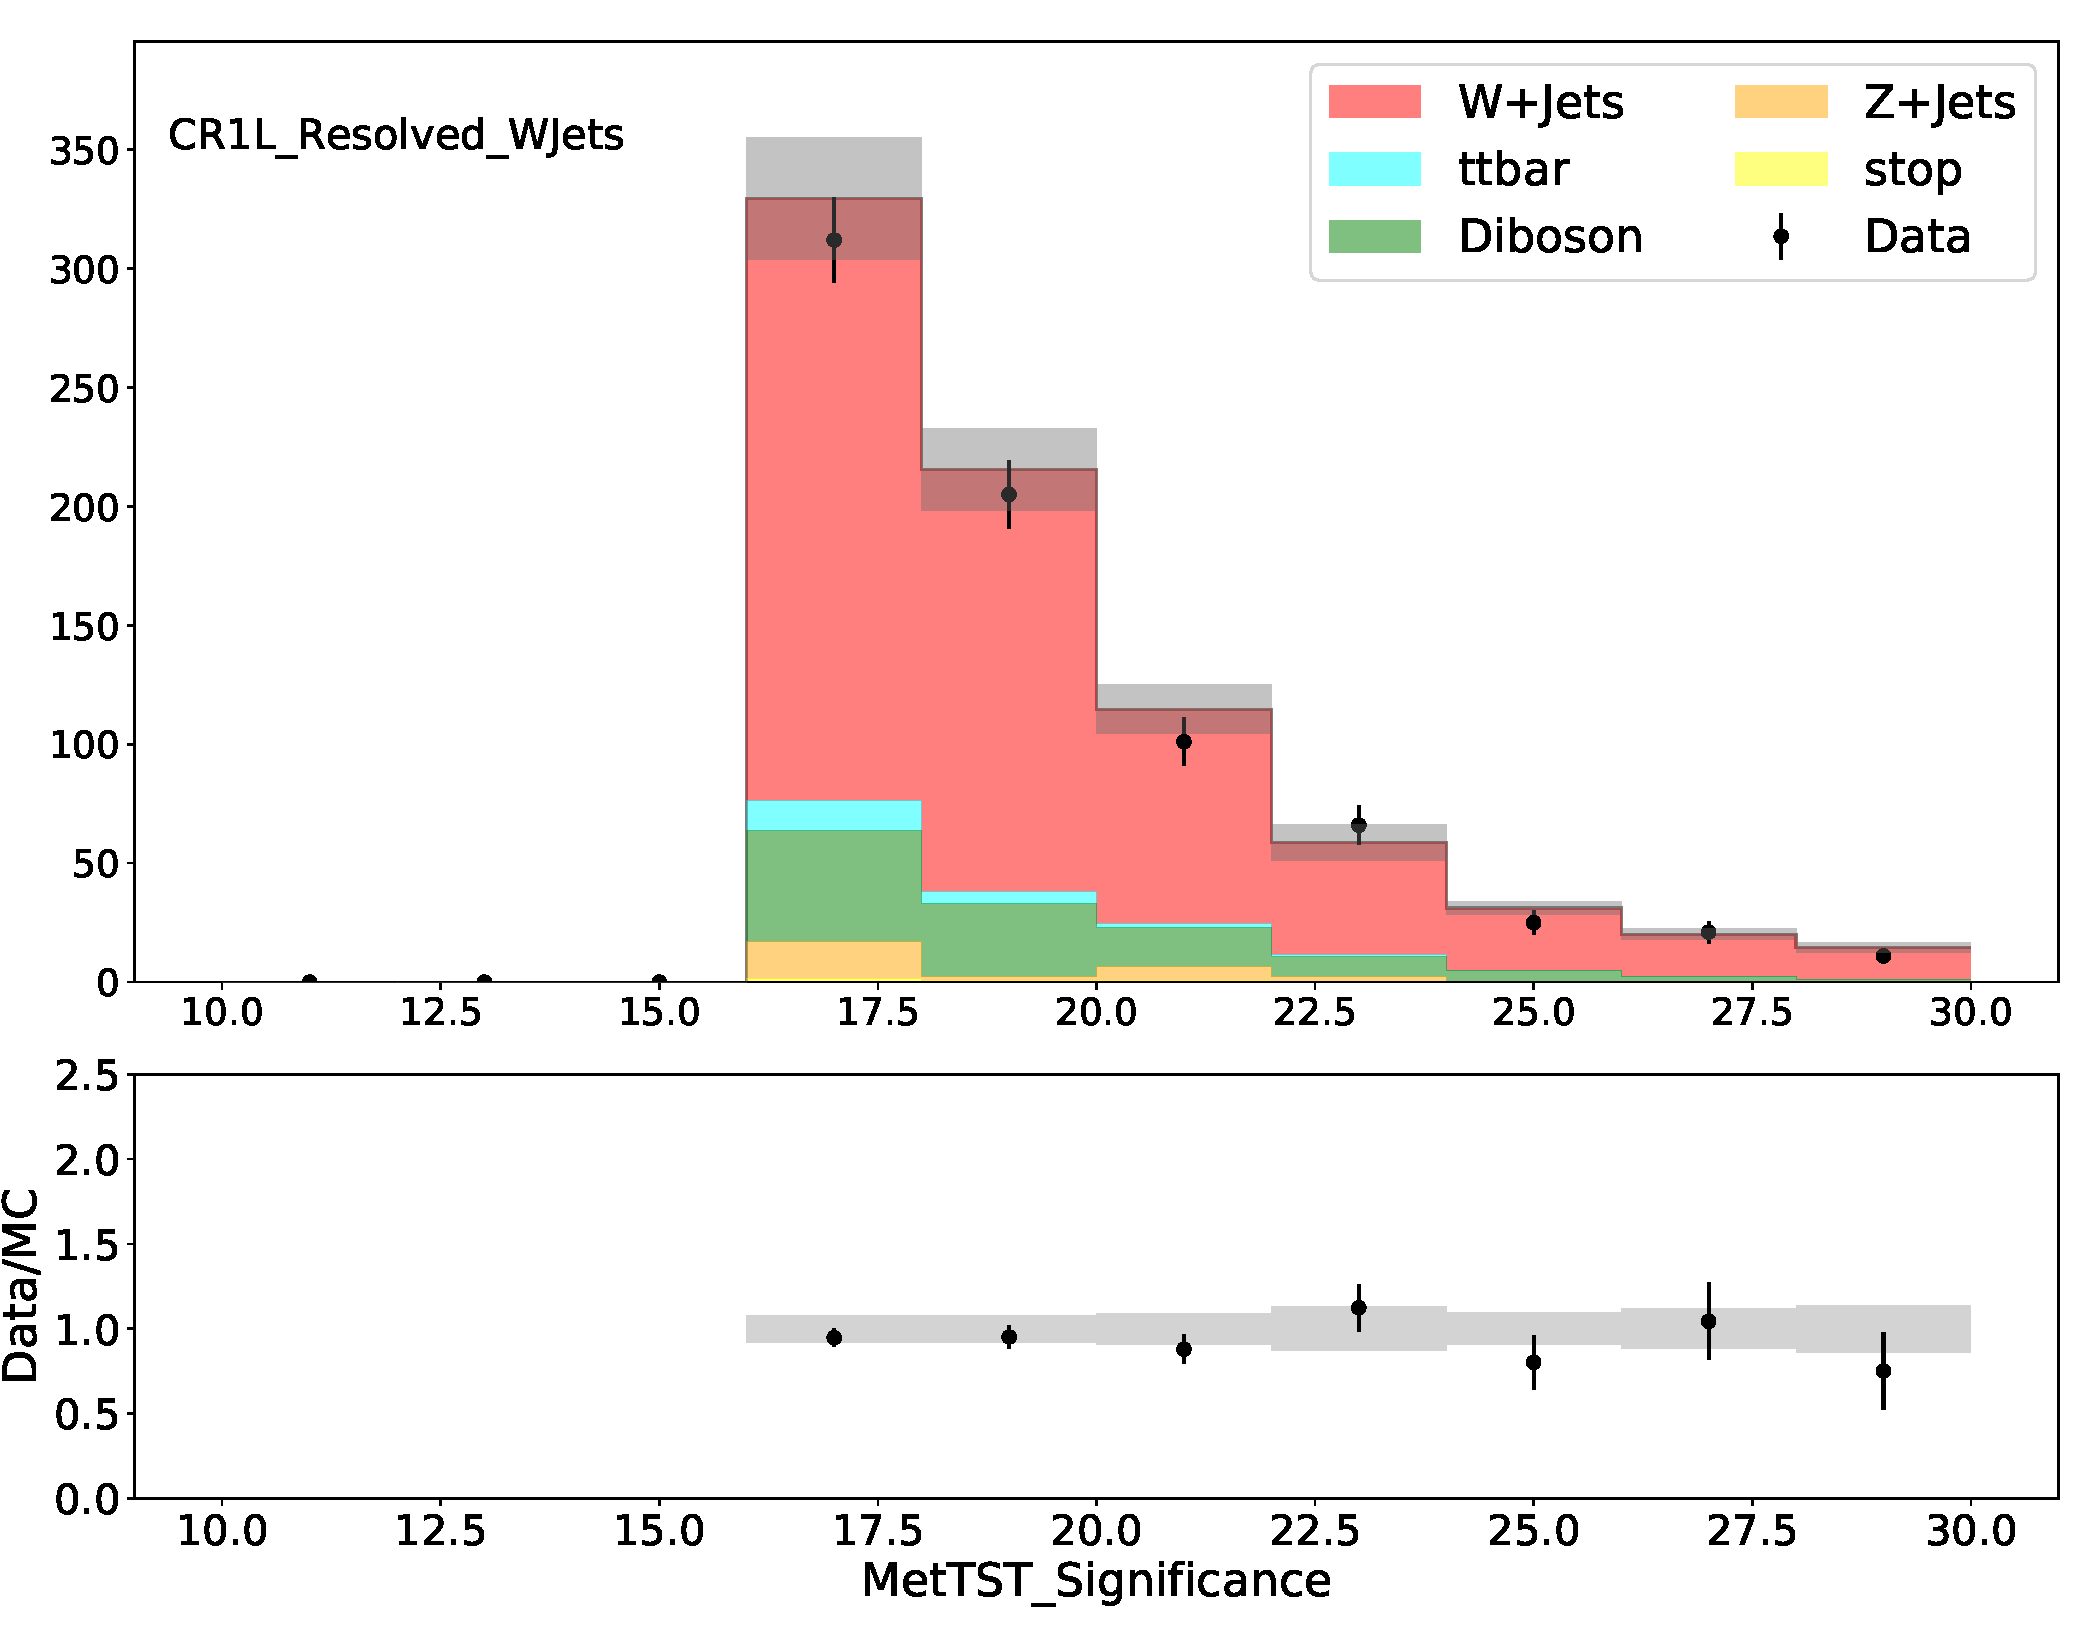
\includegraphics[width = 0.98\textwidth]{Figures/4/datamc/CR1L_Resolved_WJets/MetTST_Significance.pdf}
     \caption{\metsig}
     \end{subfigure}
     \begin{subfigure}{0.49\textwidth}
     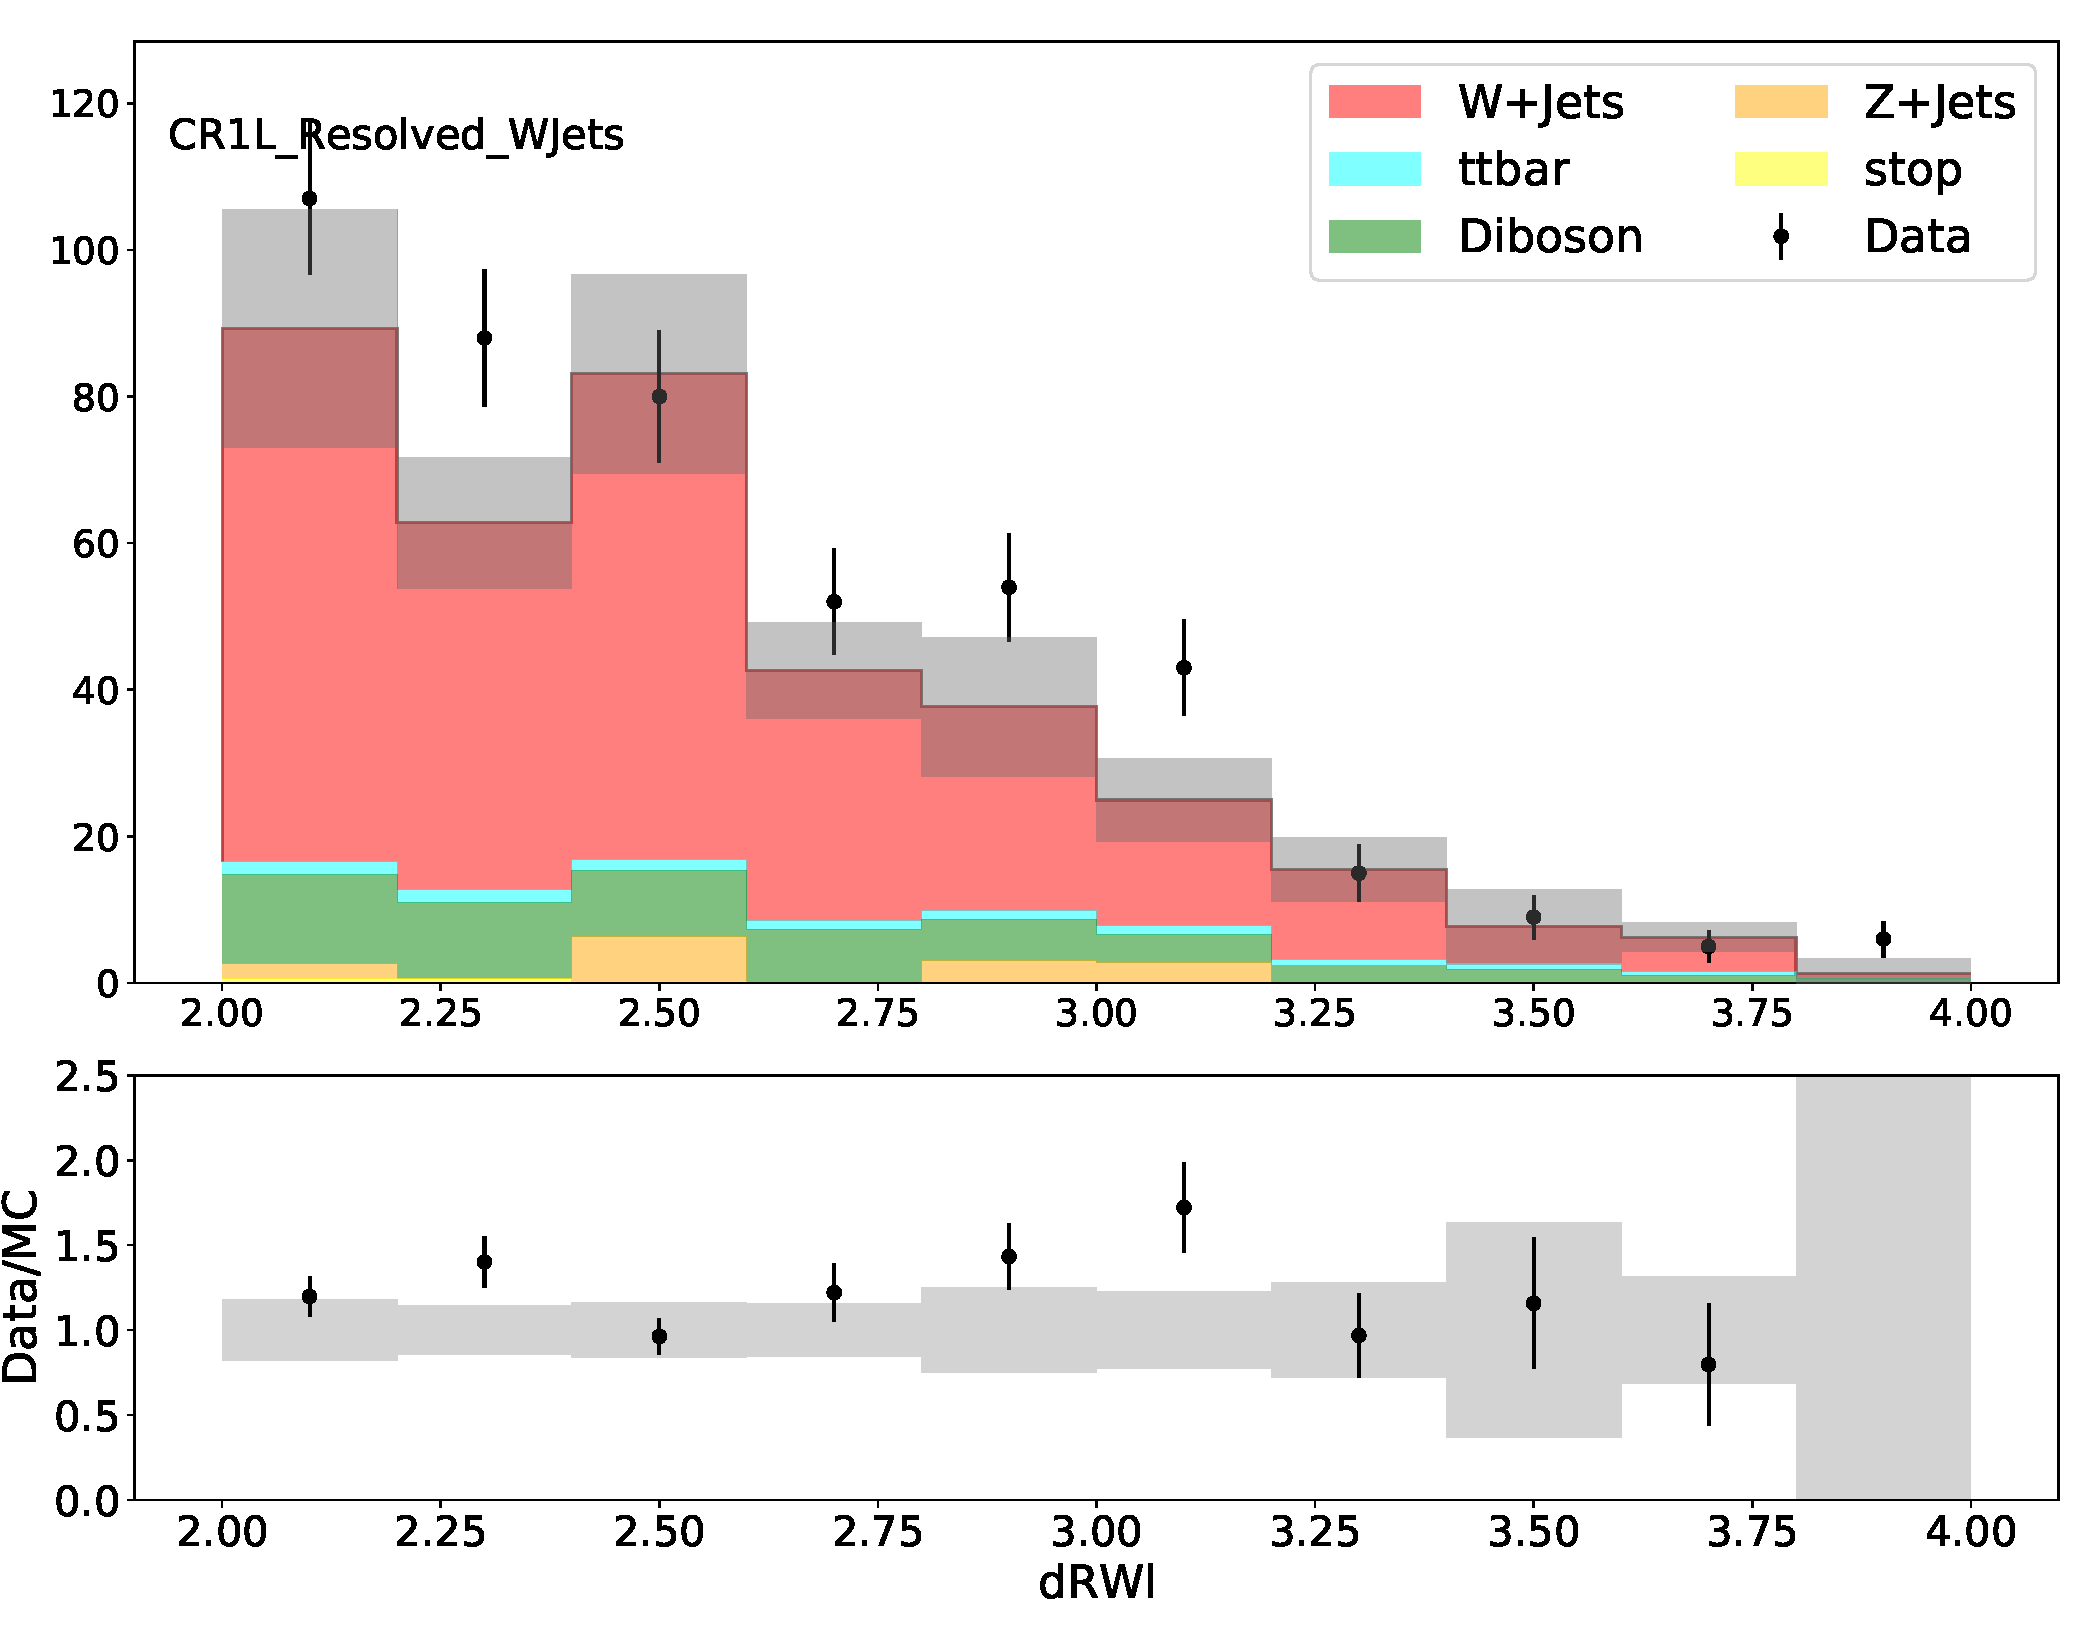
\includegraphics[width = 0.98\textwidth]{Figures/4/datamc/CR1L_Resolved_WJets/dRWl.pdf}
     \caption{\drWl}
     \end{subfigure}
     \caption{Data-MC comparisons in the \resolved \wjets control region. Grey bands represent MC statistical uncertainty on each bin.}
     \label{fig:Data_MC_CRdR_resolved}
  \end{figure}
  \begin{figure}[htbp]
    \centering
     \begin{subfigure}{0.49\textwidth}
     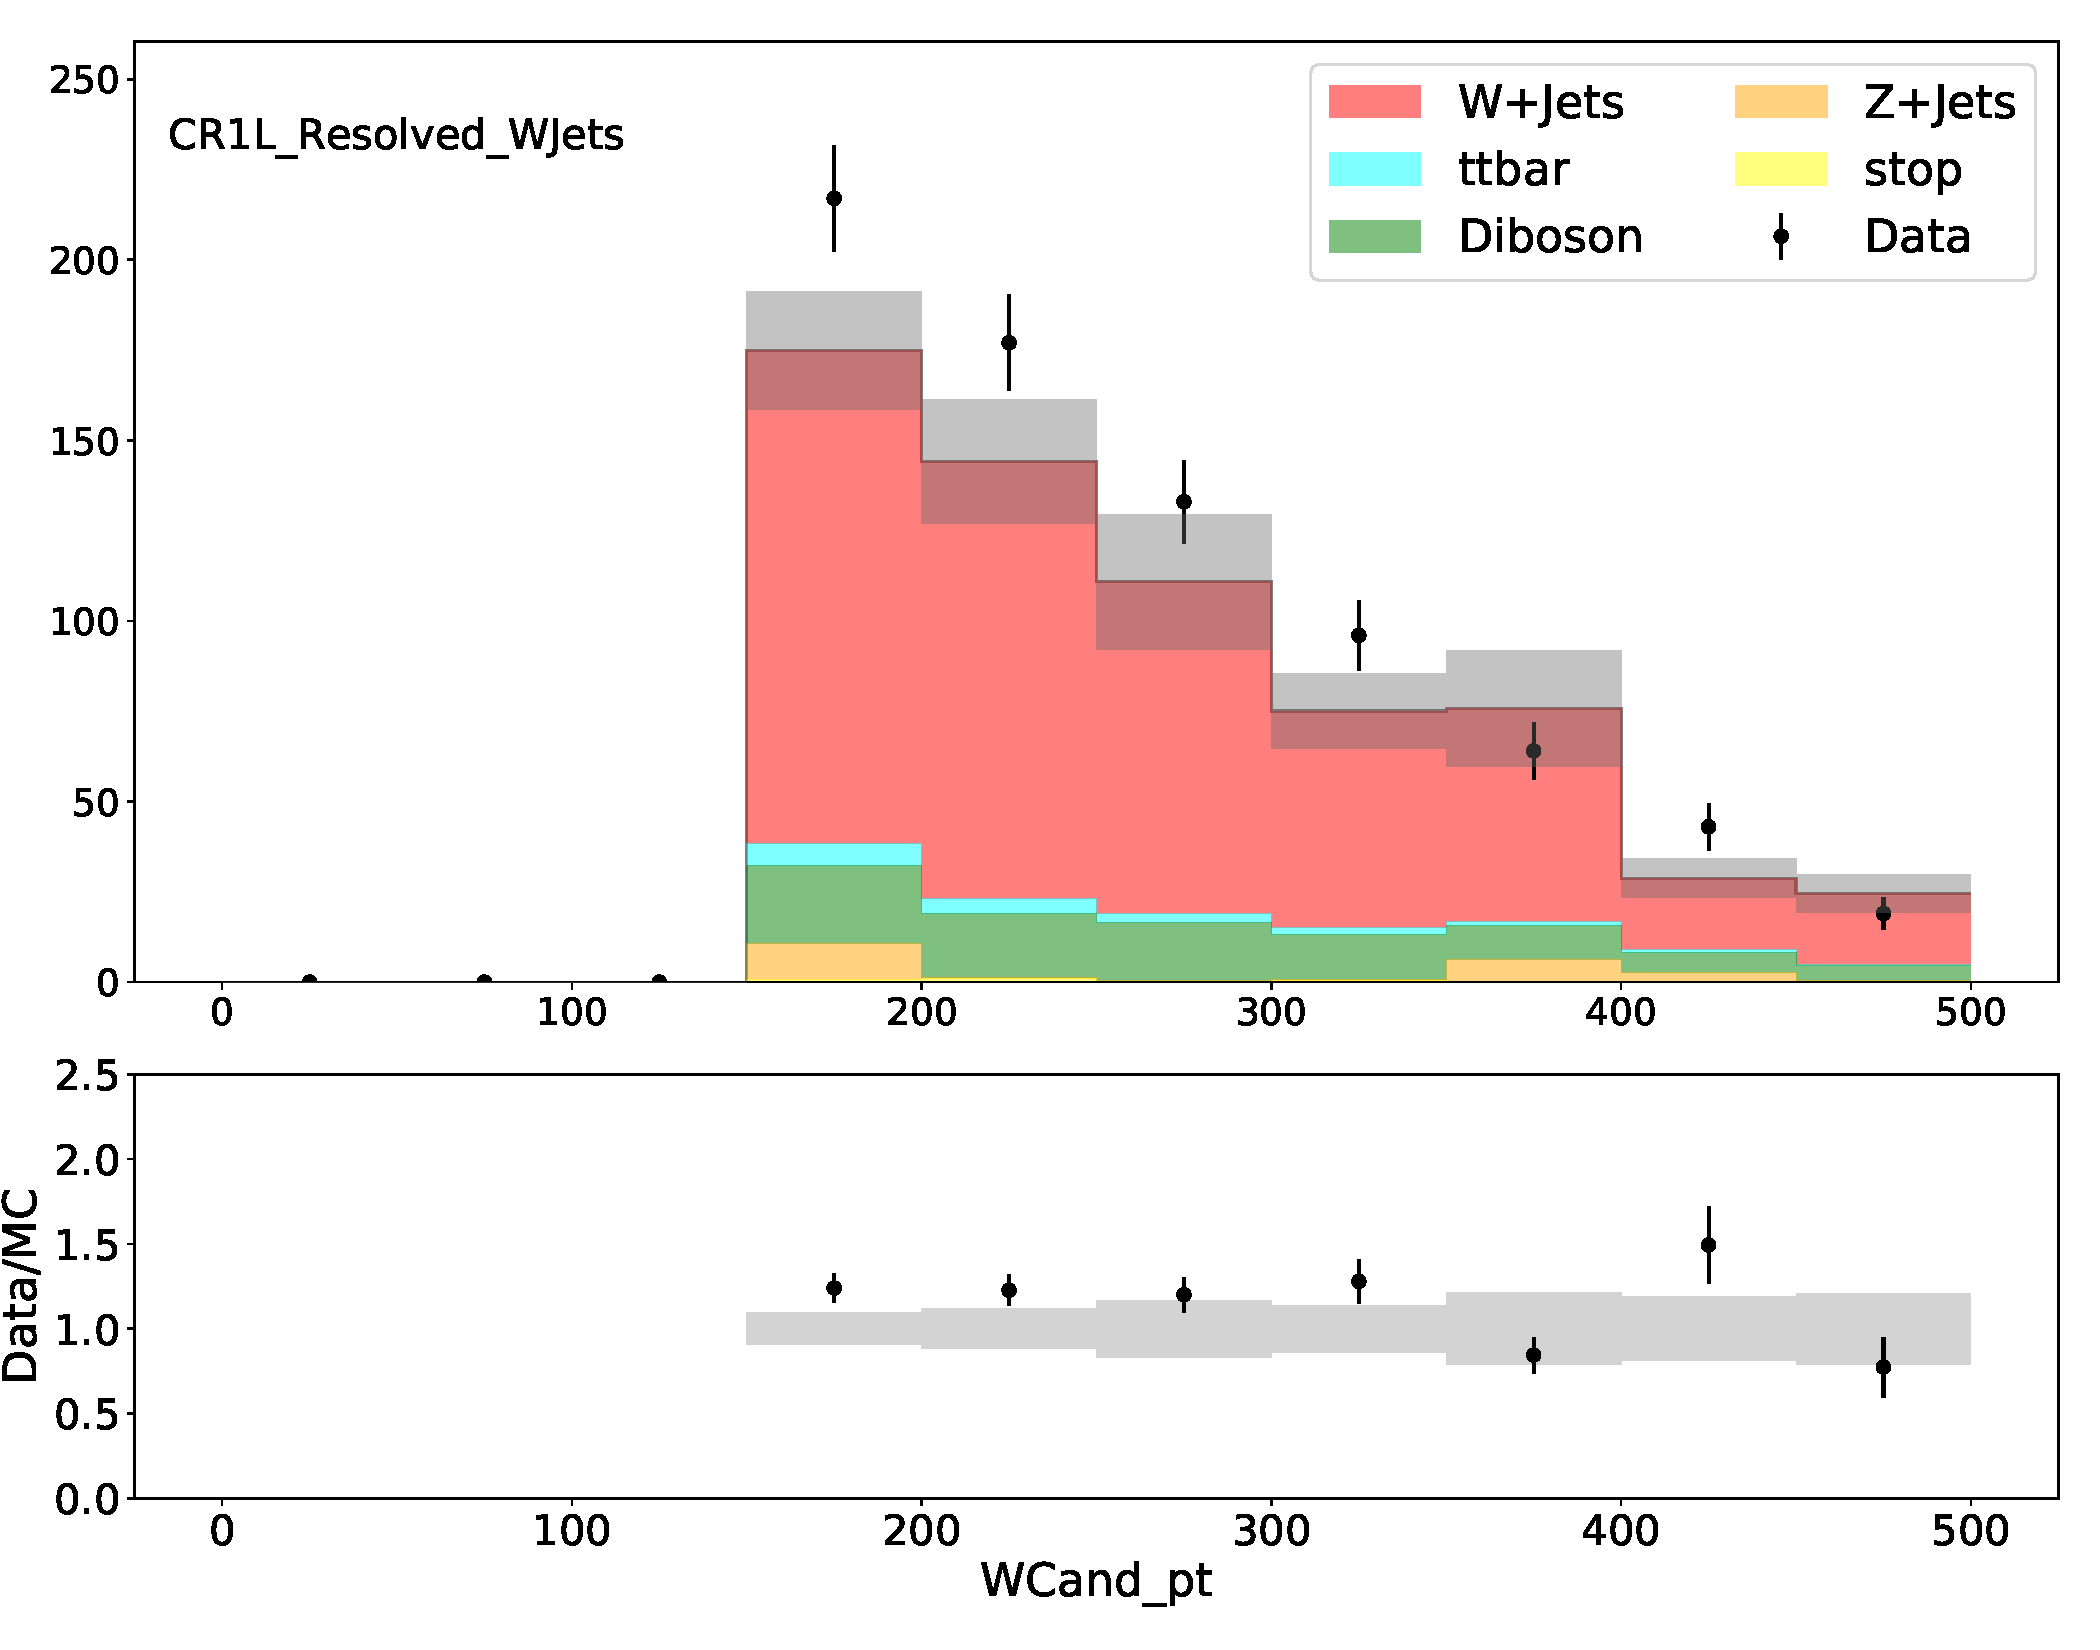
\includegraphics[width = 0.98\textwidth]{Figures/4/datamc/CR1L_Resolved_WJets/WCand_pt.pdf}
     \caption{\Wcandpt}
     \end{subfigure}
     \begin{subfigure}{0.49\textwidth}
     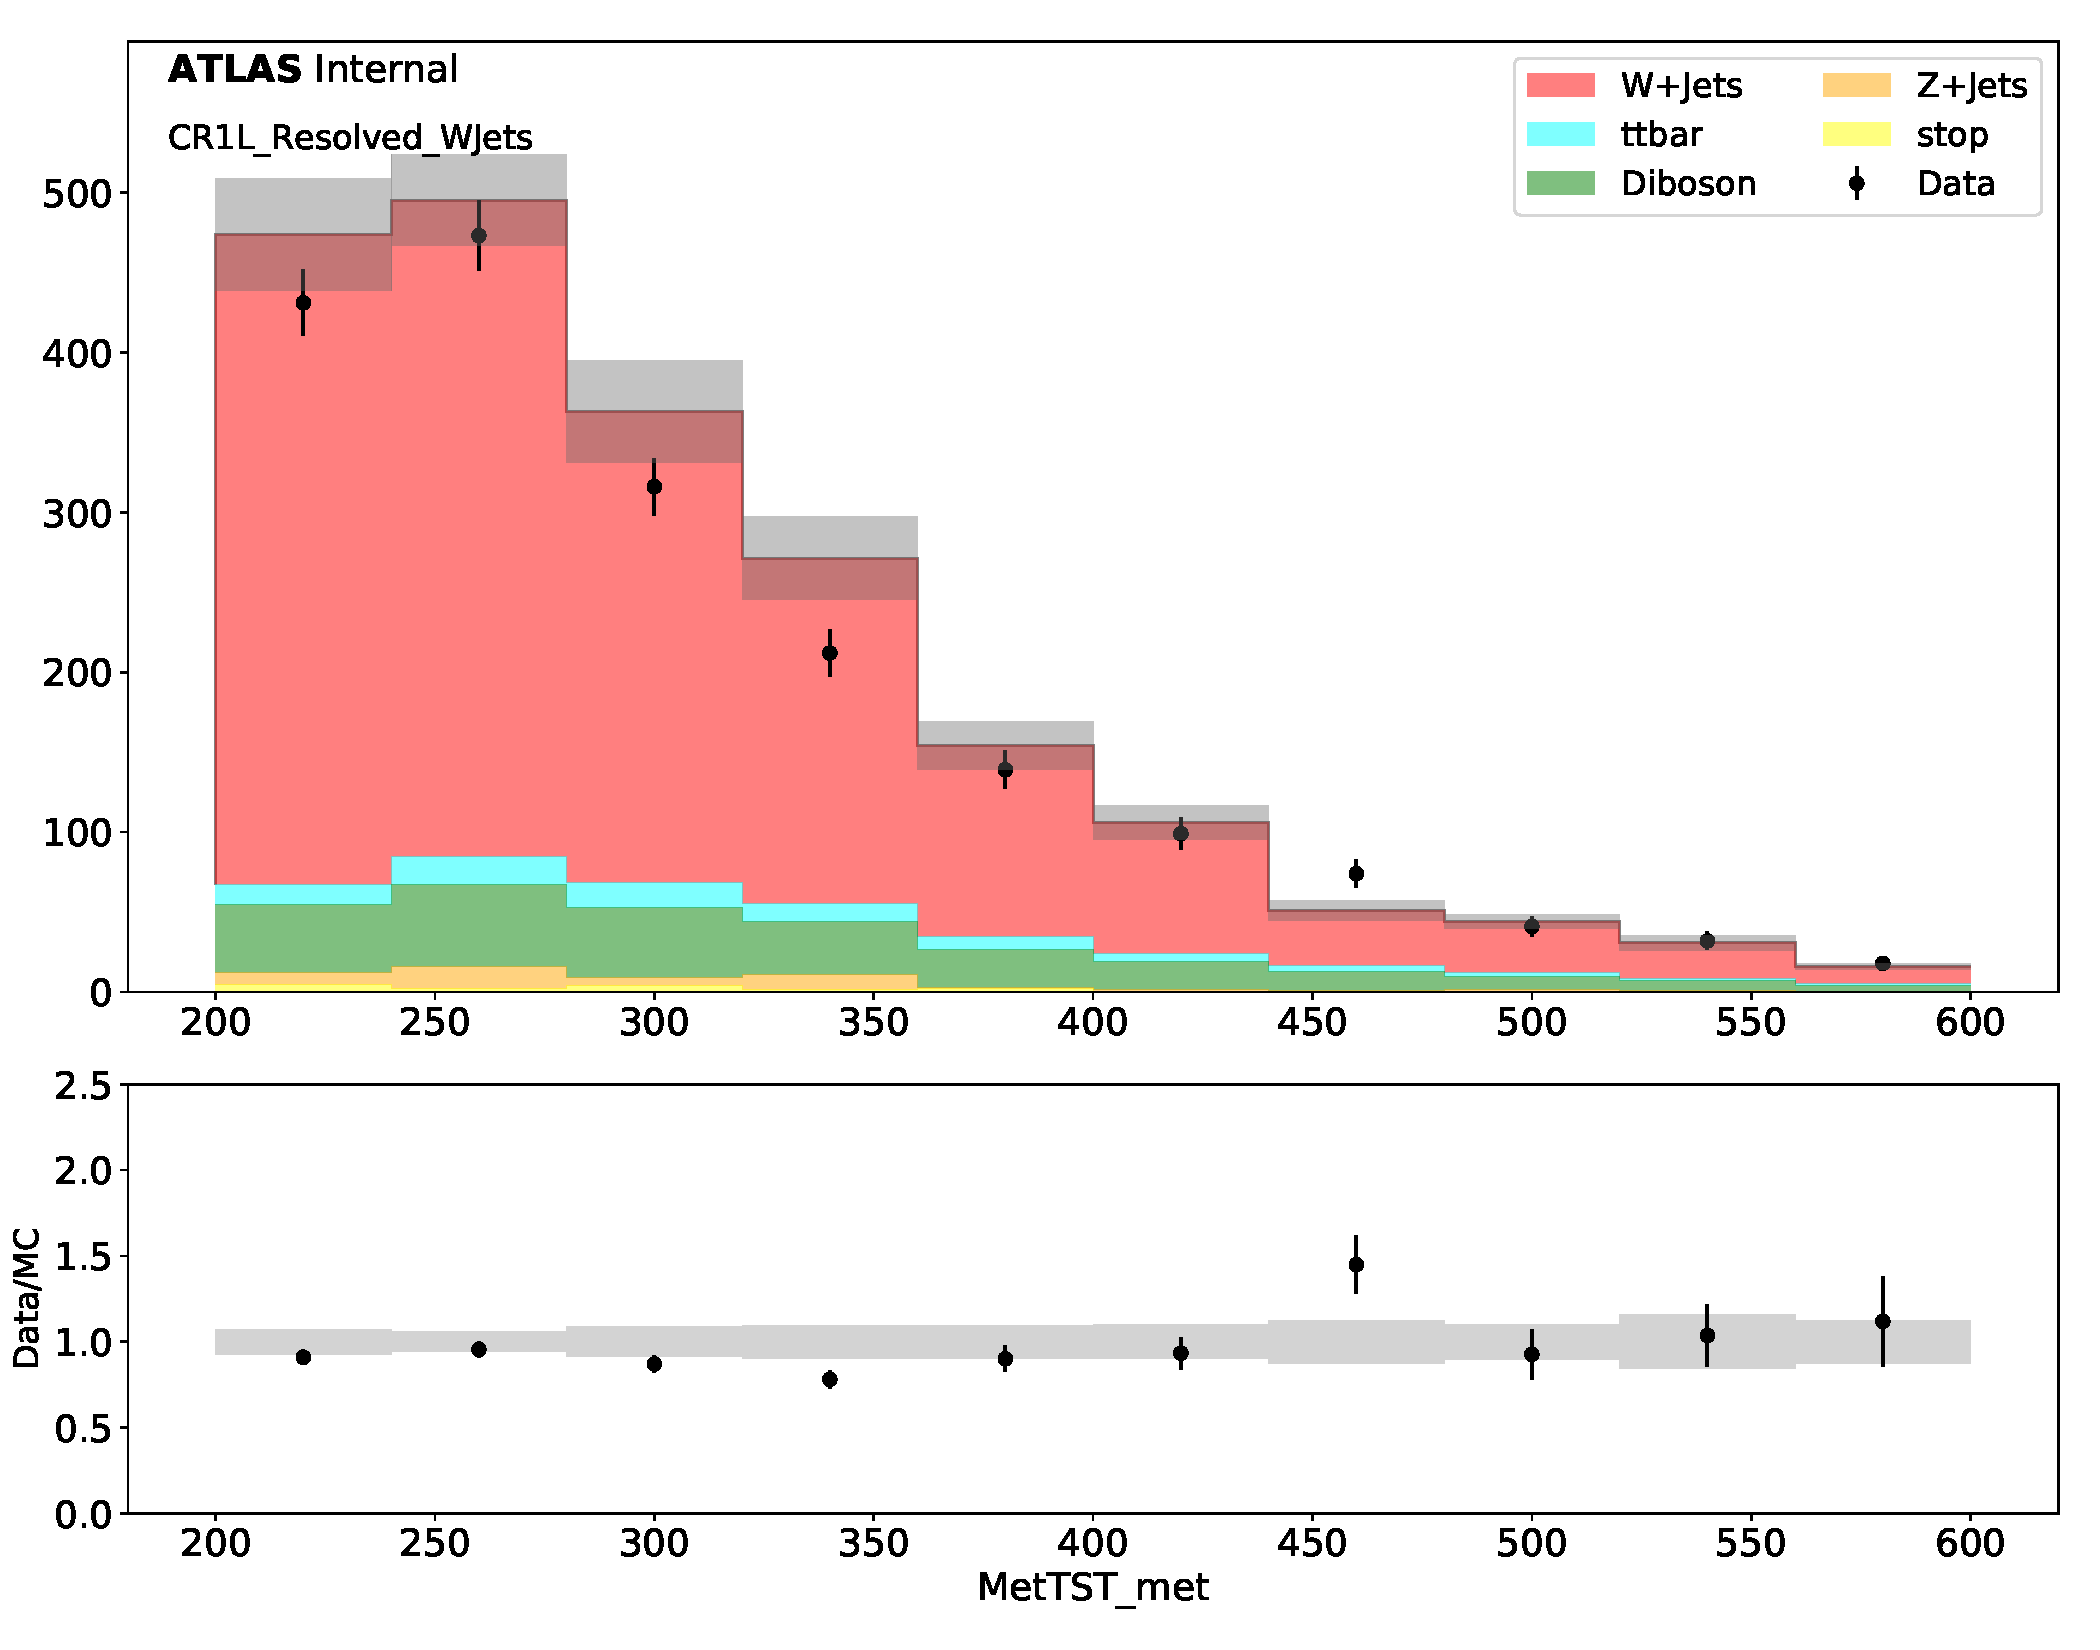
\includegraphics[width = 0.98\textwidth]{Figures/4/datamc/CR1L_Resolved_WJets/MetTST_met.pdf}
     \caption{\met}
     \end{subfigure}

     \caption{Data-MC comparisons in the \resolved \wjets control region. Grey bands represent MC statistical uncertainty on each bin.}
     \label{fig:Data_MC_CRdR_resolved}
  \end{figure}

\FloatBarrier

\section{CR-SR Distribution Comparisons}
\label{section:CRSR}

\begin{figure}[htbp]
  \centering

    \begin{subfigure}{0.49\textwidth}
    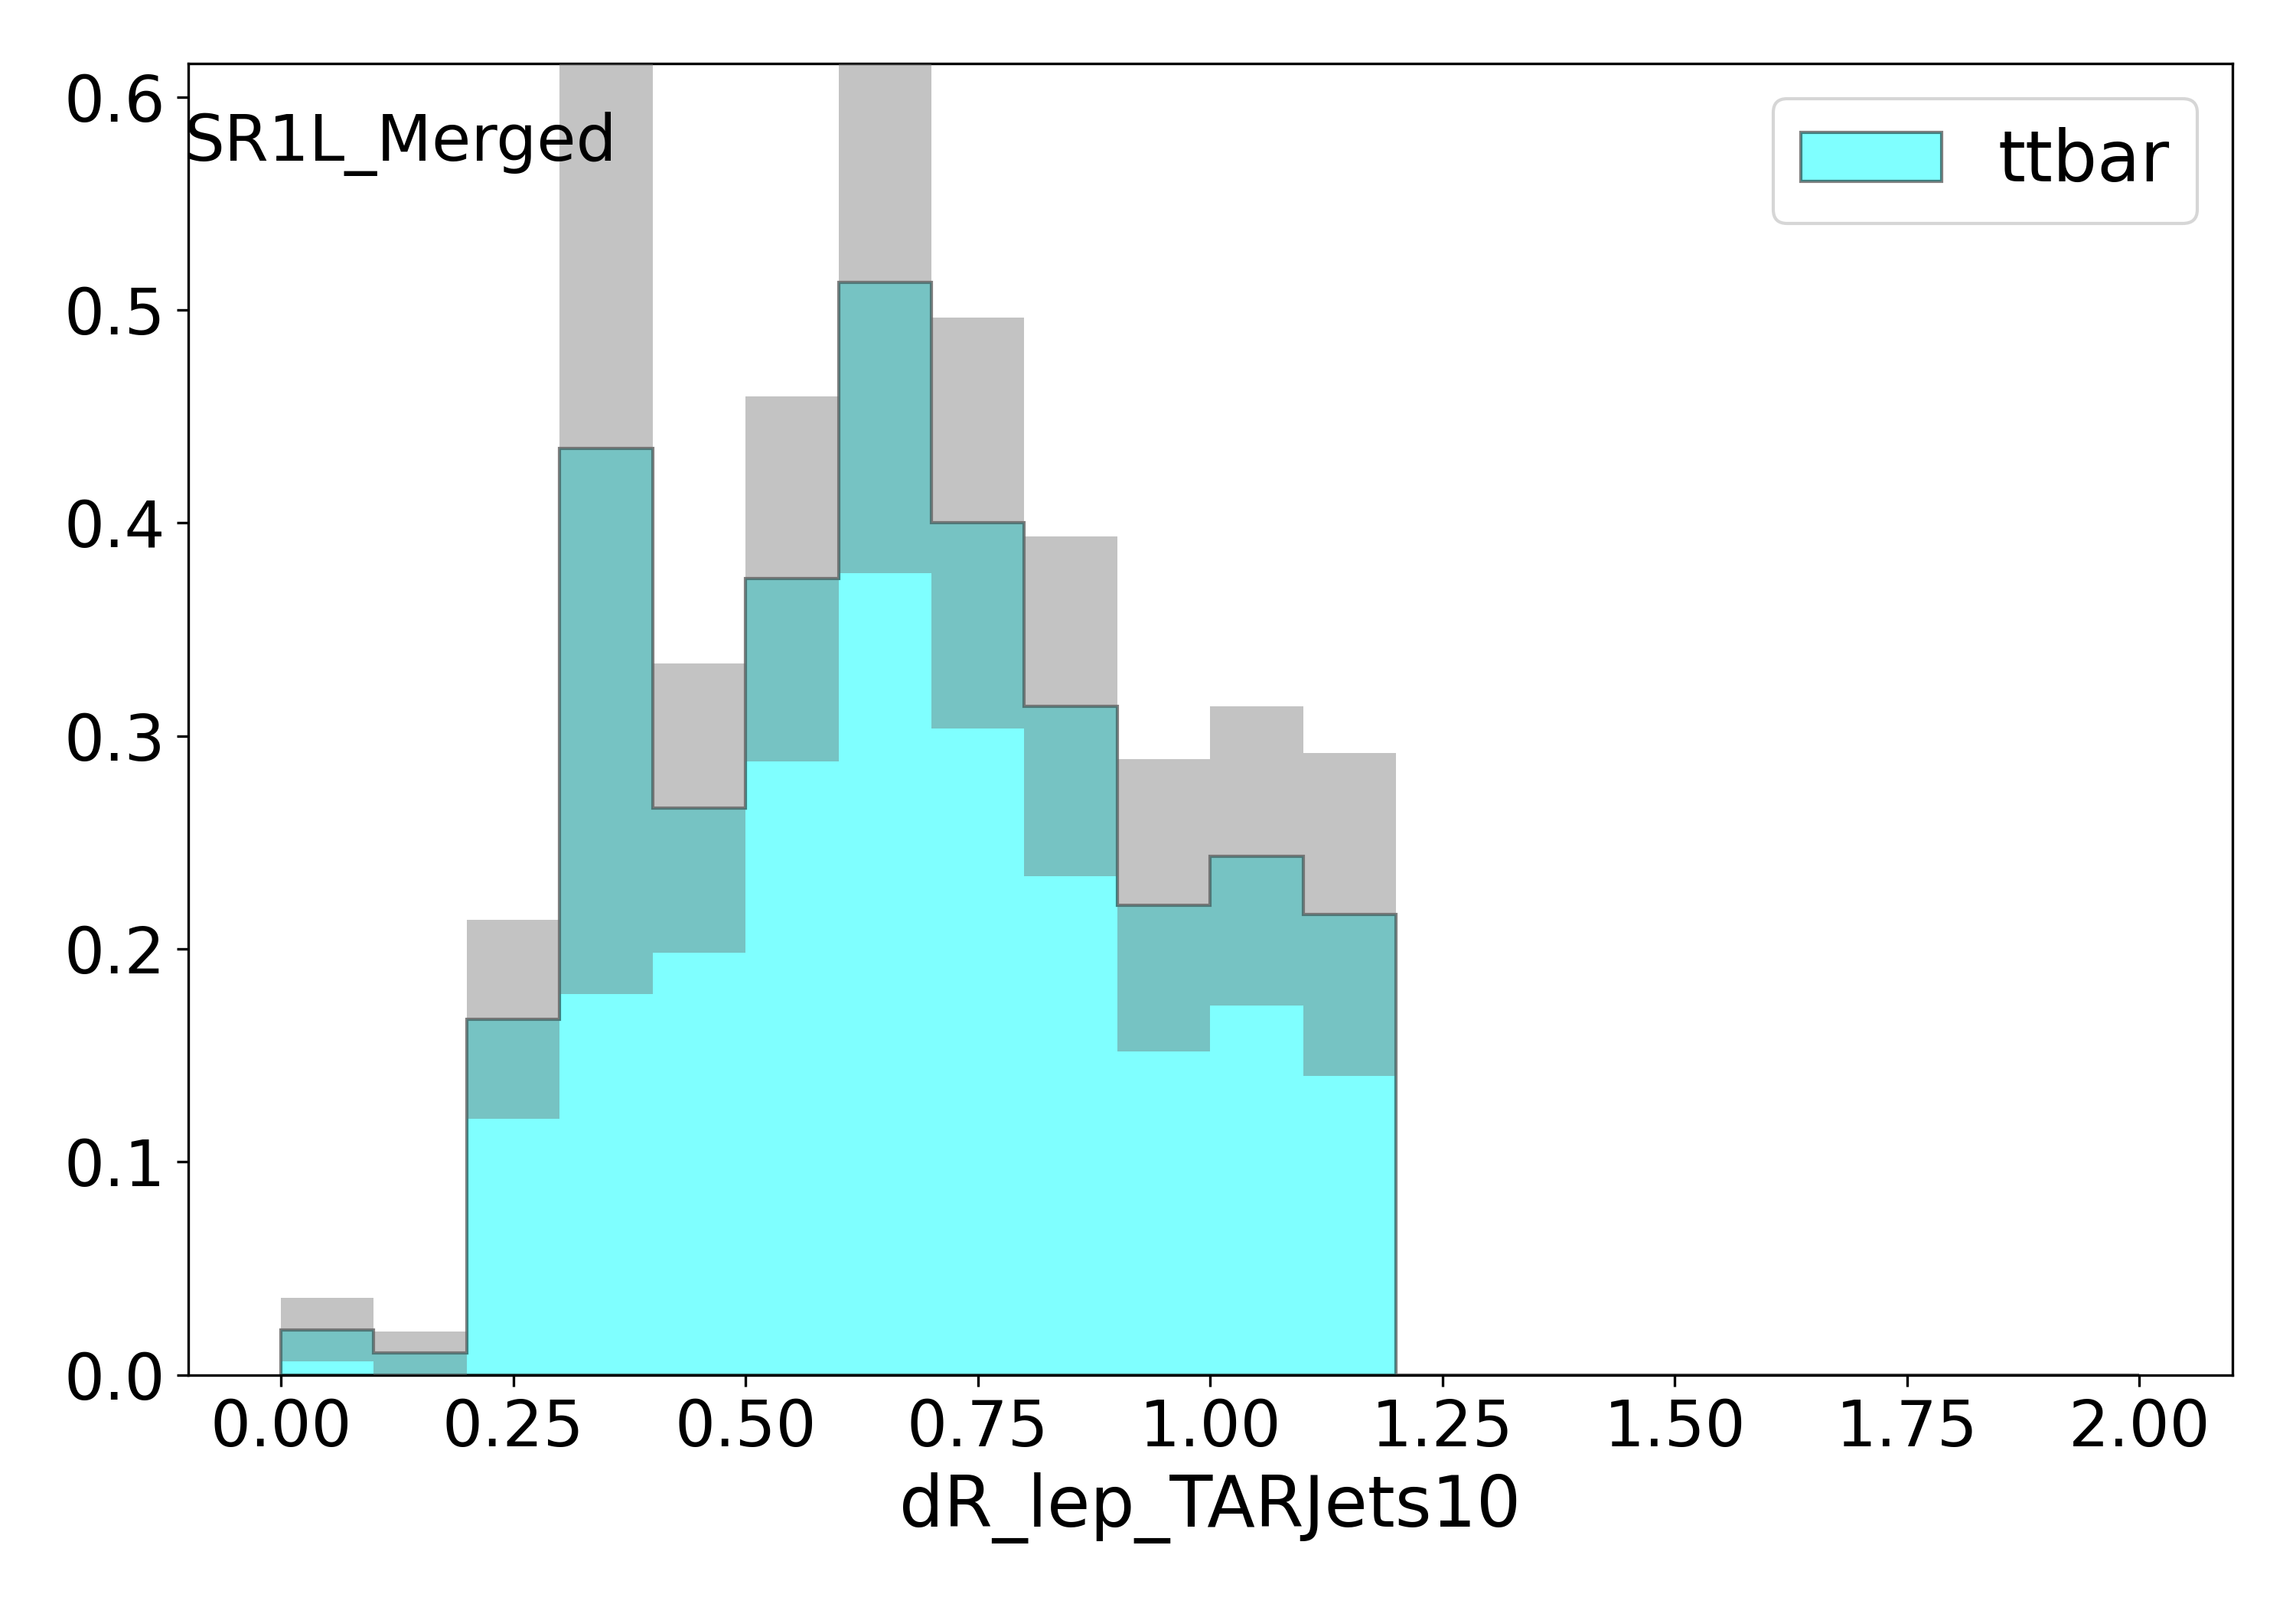
\includegraphics[width = 0.98\textwidth]{Figures/4/CRSR/SR1L_Merged/dR_lep_TARJets10.png}
    \caption{Merged SR \drTARl}
    \end{subfigure}
    \begin{subfigure}{0.49\textwidth}
    \includegraphics[width = 0.98\textwidth]{Figures/4/CRSR/CR1L_Merged_ttbar/dR_lep_TARJets10.png}
    \caption{Merged CR \drTARl}
    \end{subfigure}
    \begin{subfigure}{0.49\textwidth}
    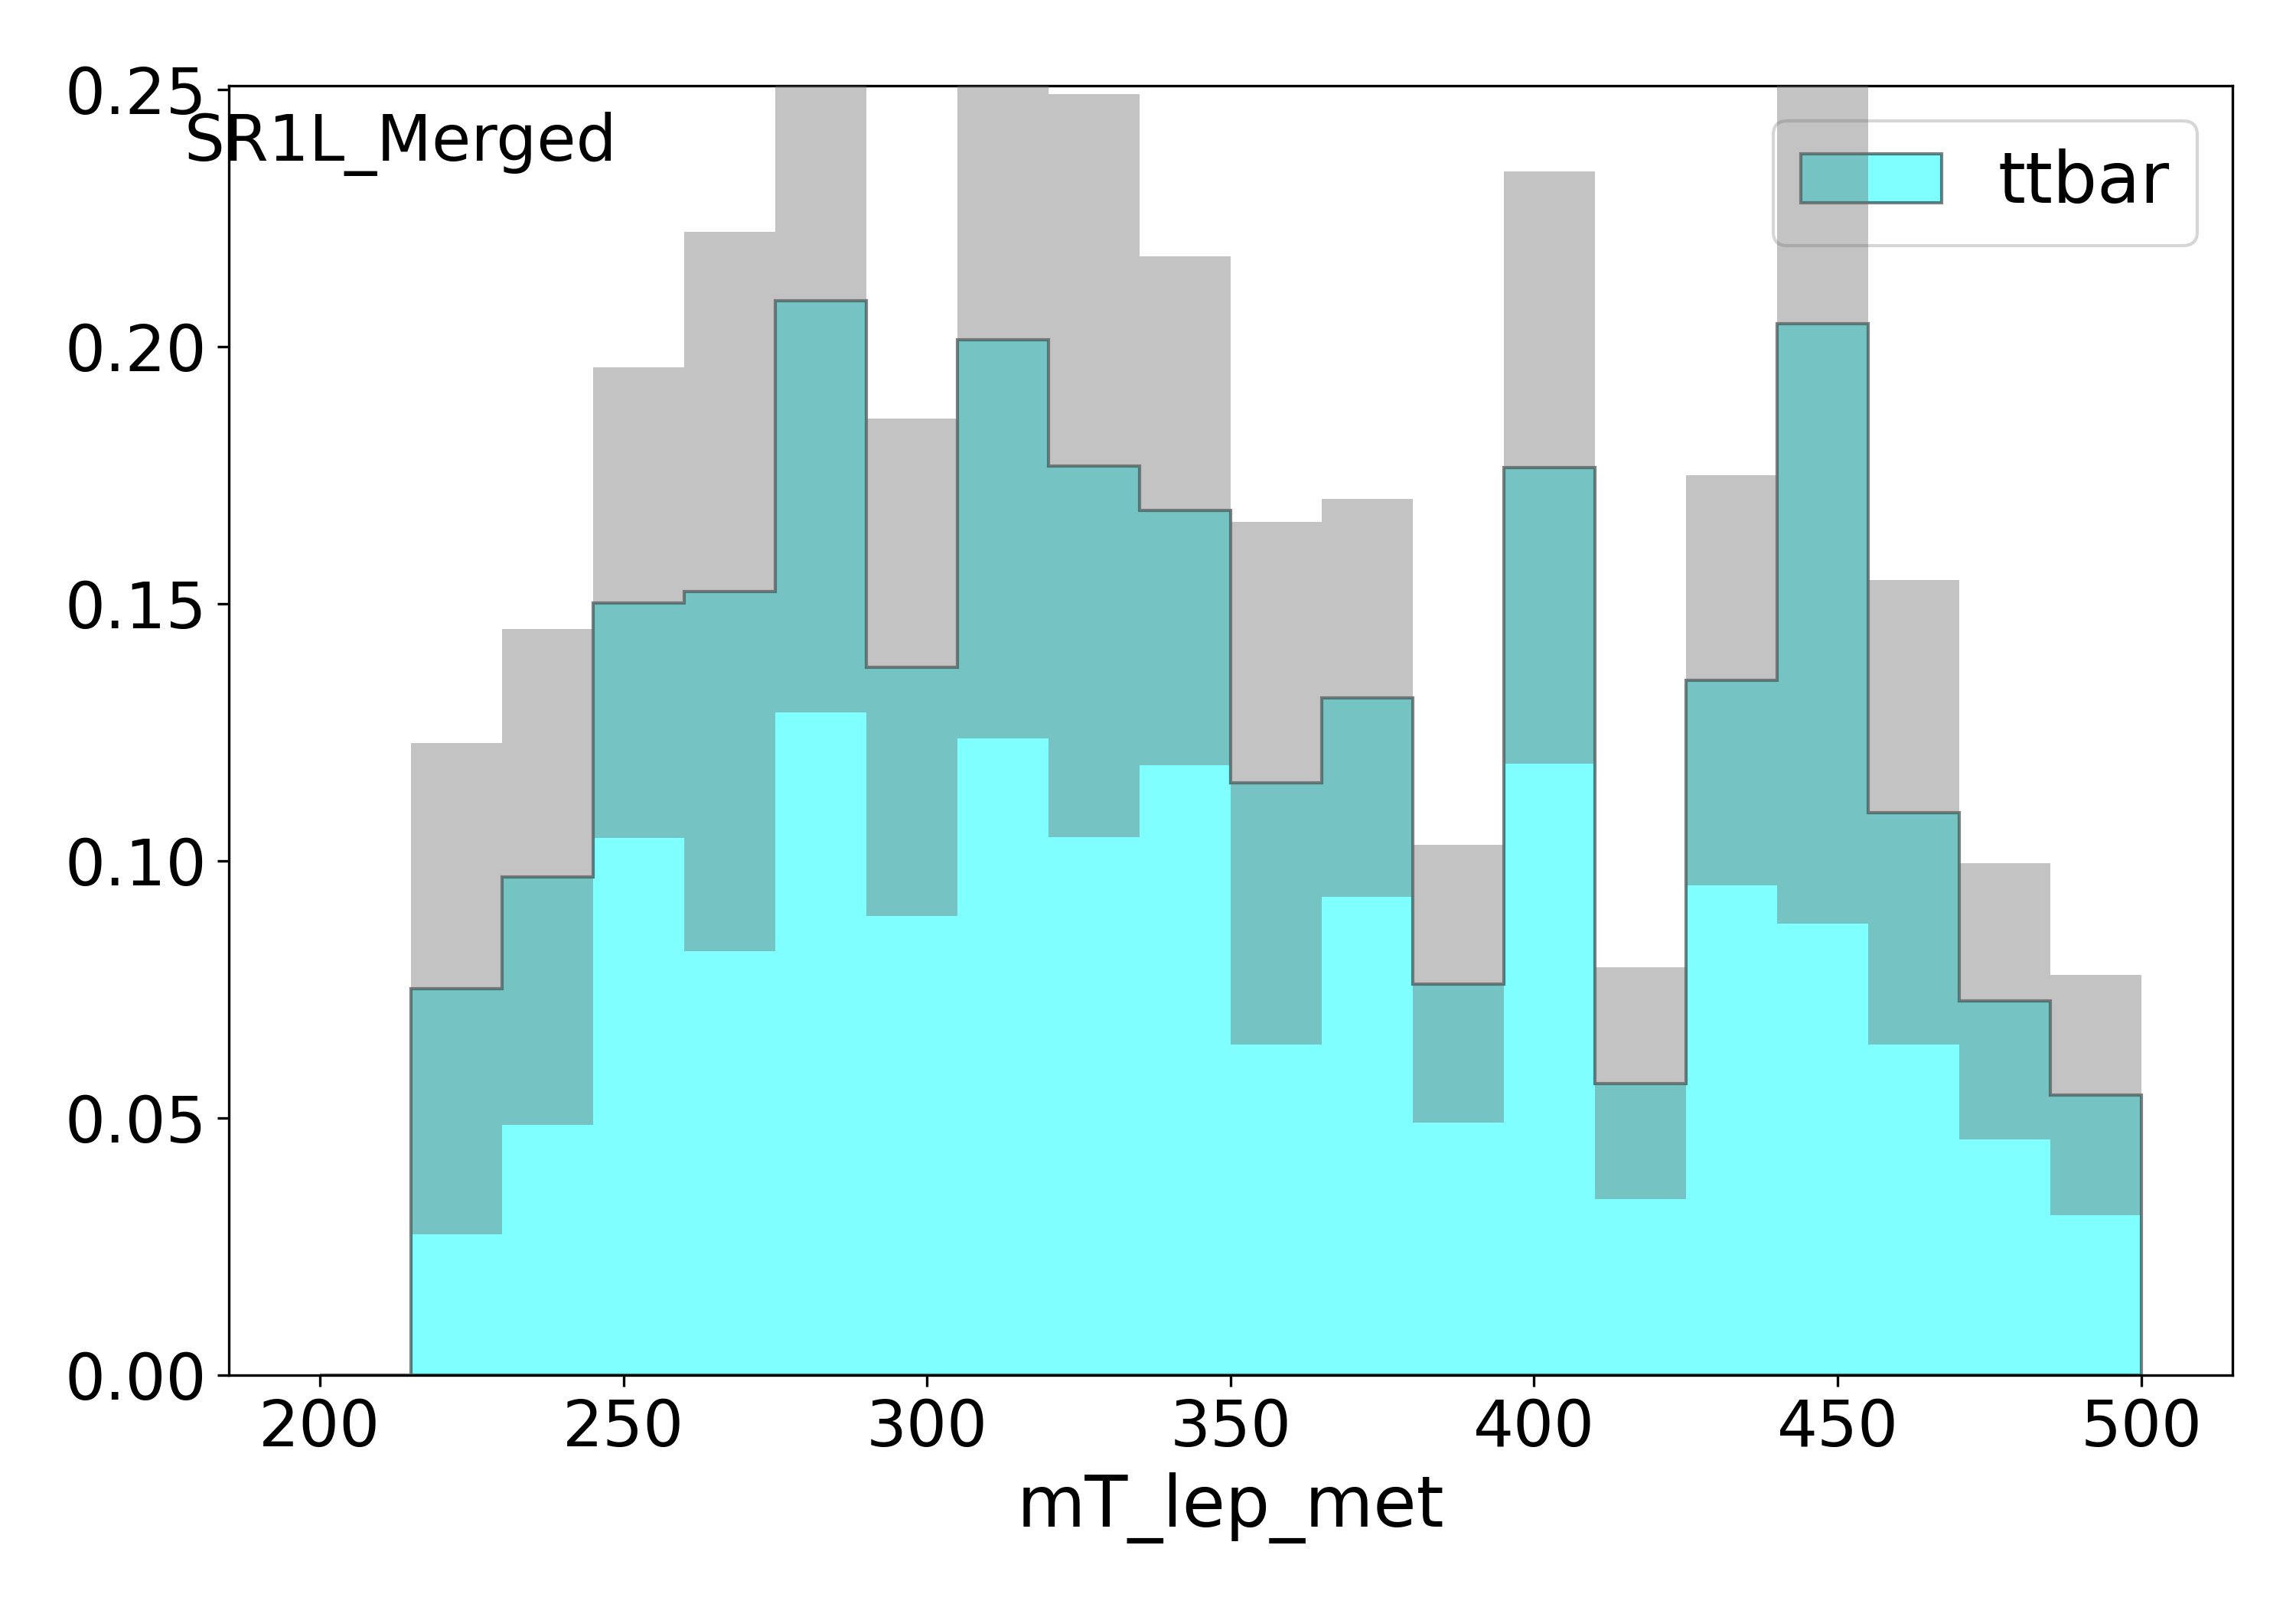
\includegraphics[width = 0.98\textwidth]{Figures/4/CRSR/SR1L_Merged/mT_lep_met.png}
    \caption{Merged SR \mtlepmet}
    \end{subfigure}
    \begin{subfigure}{0.49\textwidth}
    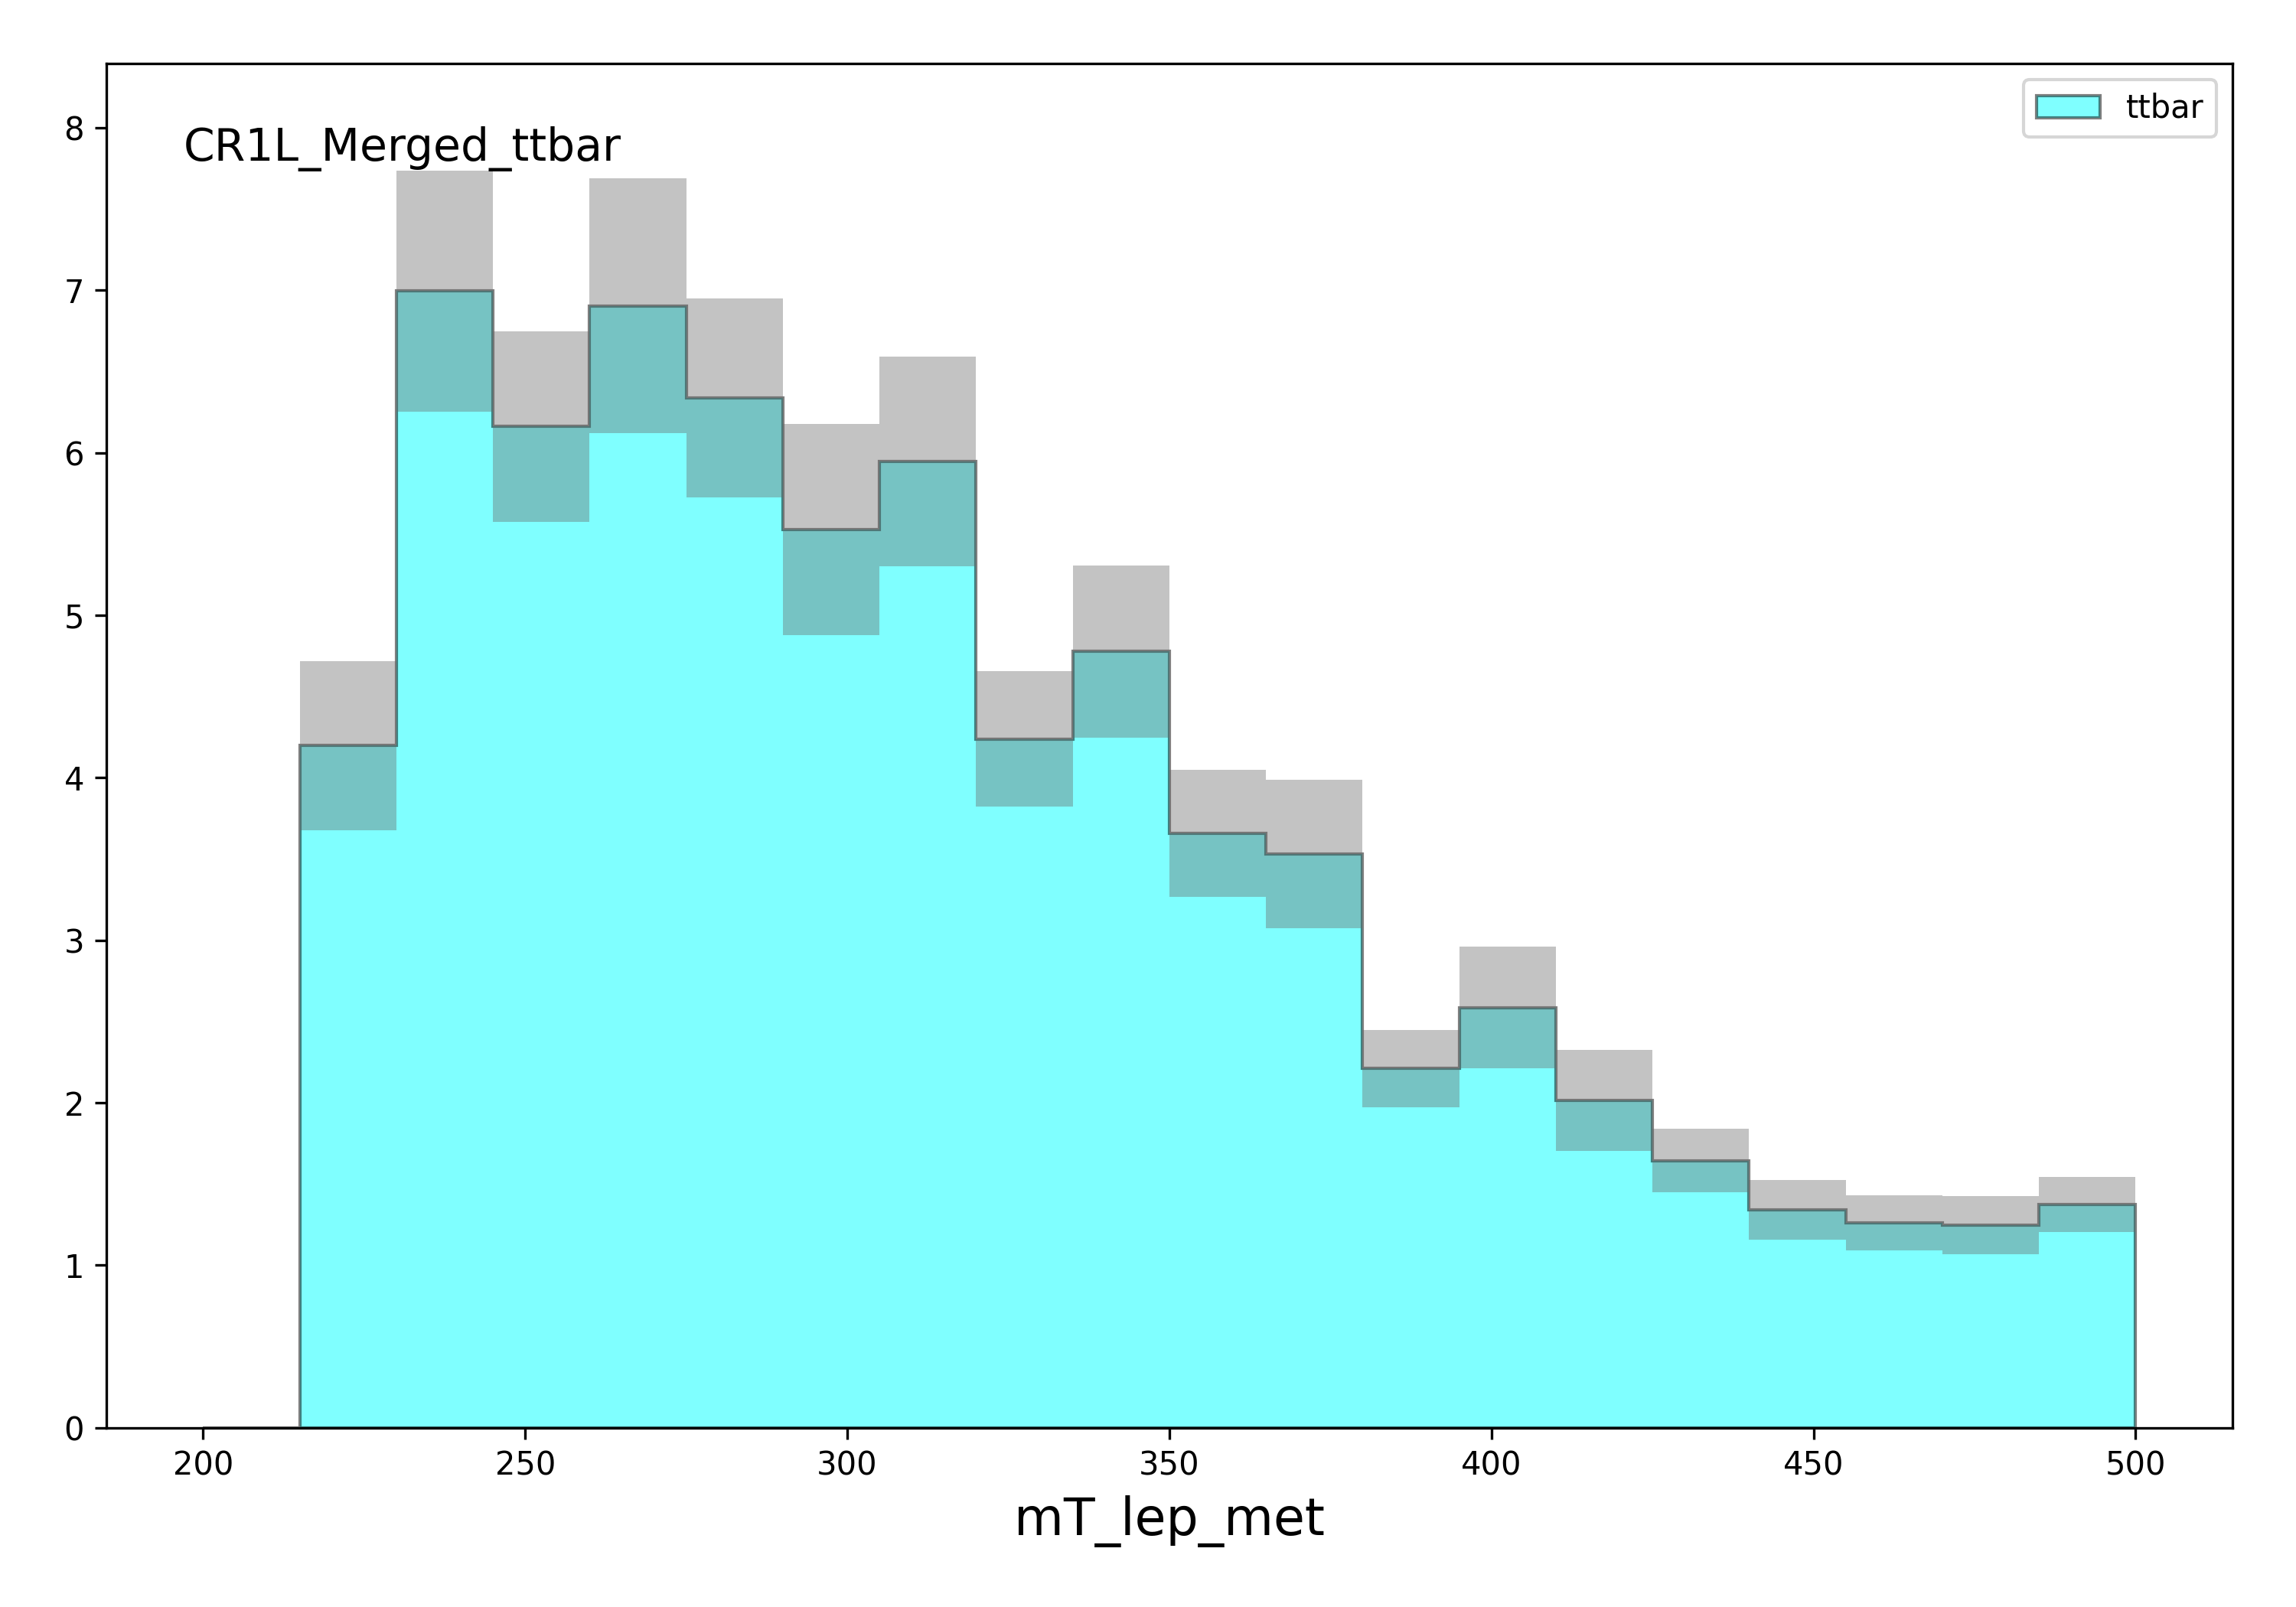
\includegraphics[width = 0.98\textwidth]{Figures/4/CRSR/CR1L_Merged_ttbar/mT_lep_met.png}
    \caption{Merged CR \mtlepmet}
    \end{subfigure}
    \caption{Comparisons of kinematic variables between the \merged signal region and \ttbar control region. \textbf{Left column:} signal region, \textbf{Right column:} control region. Grey bands represent MC statistical uncertainty on each bin.}
    \label{fig:CRSR_merged}
 \end{figure}

 \begin{figure}[htbp]
   \centering
    \begin{subfigure}{0.49\textwidth}
    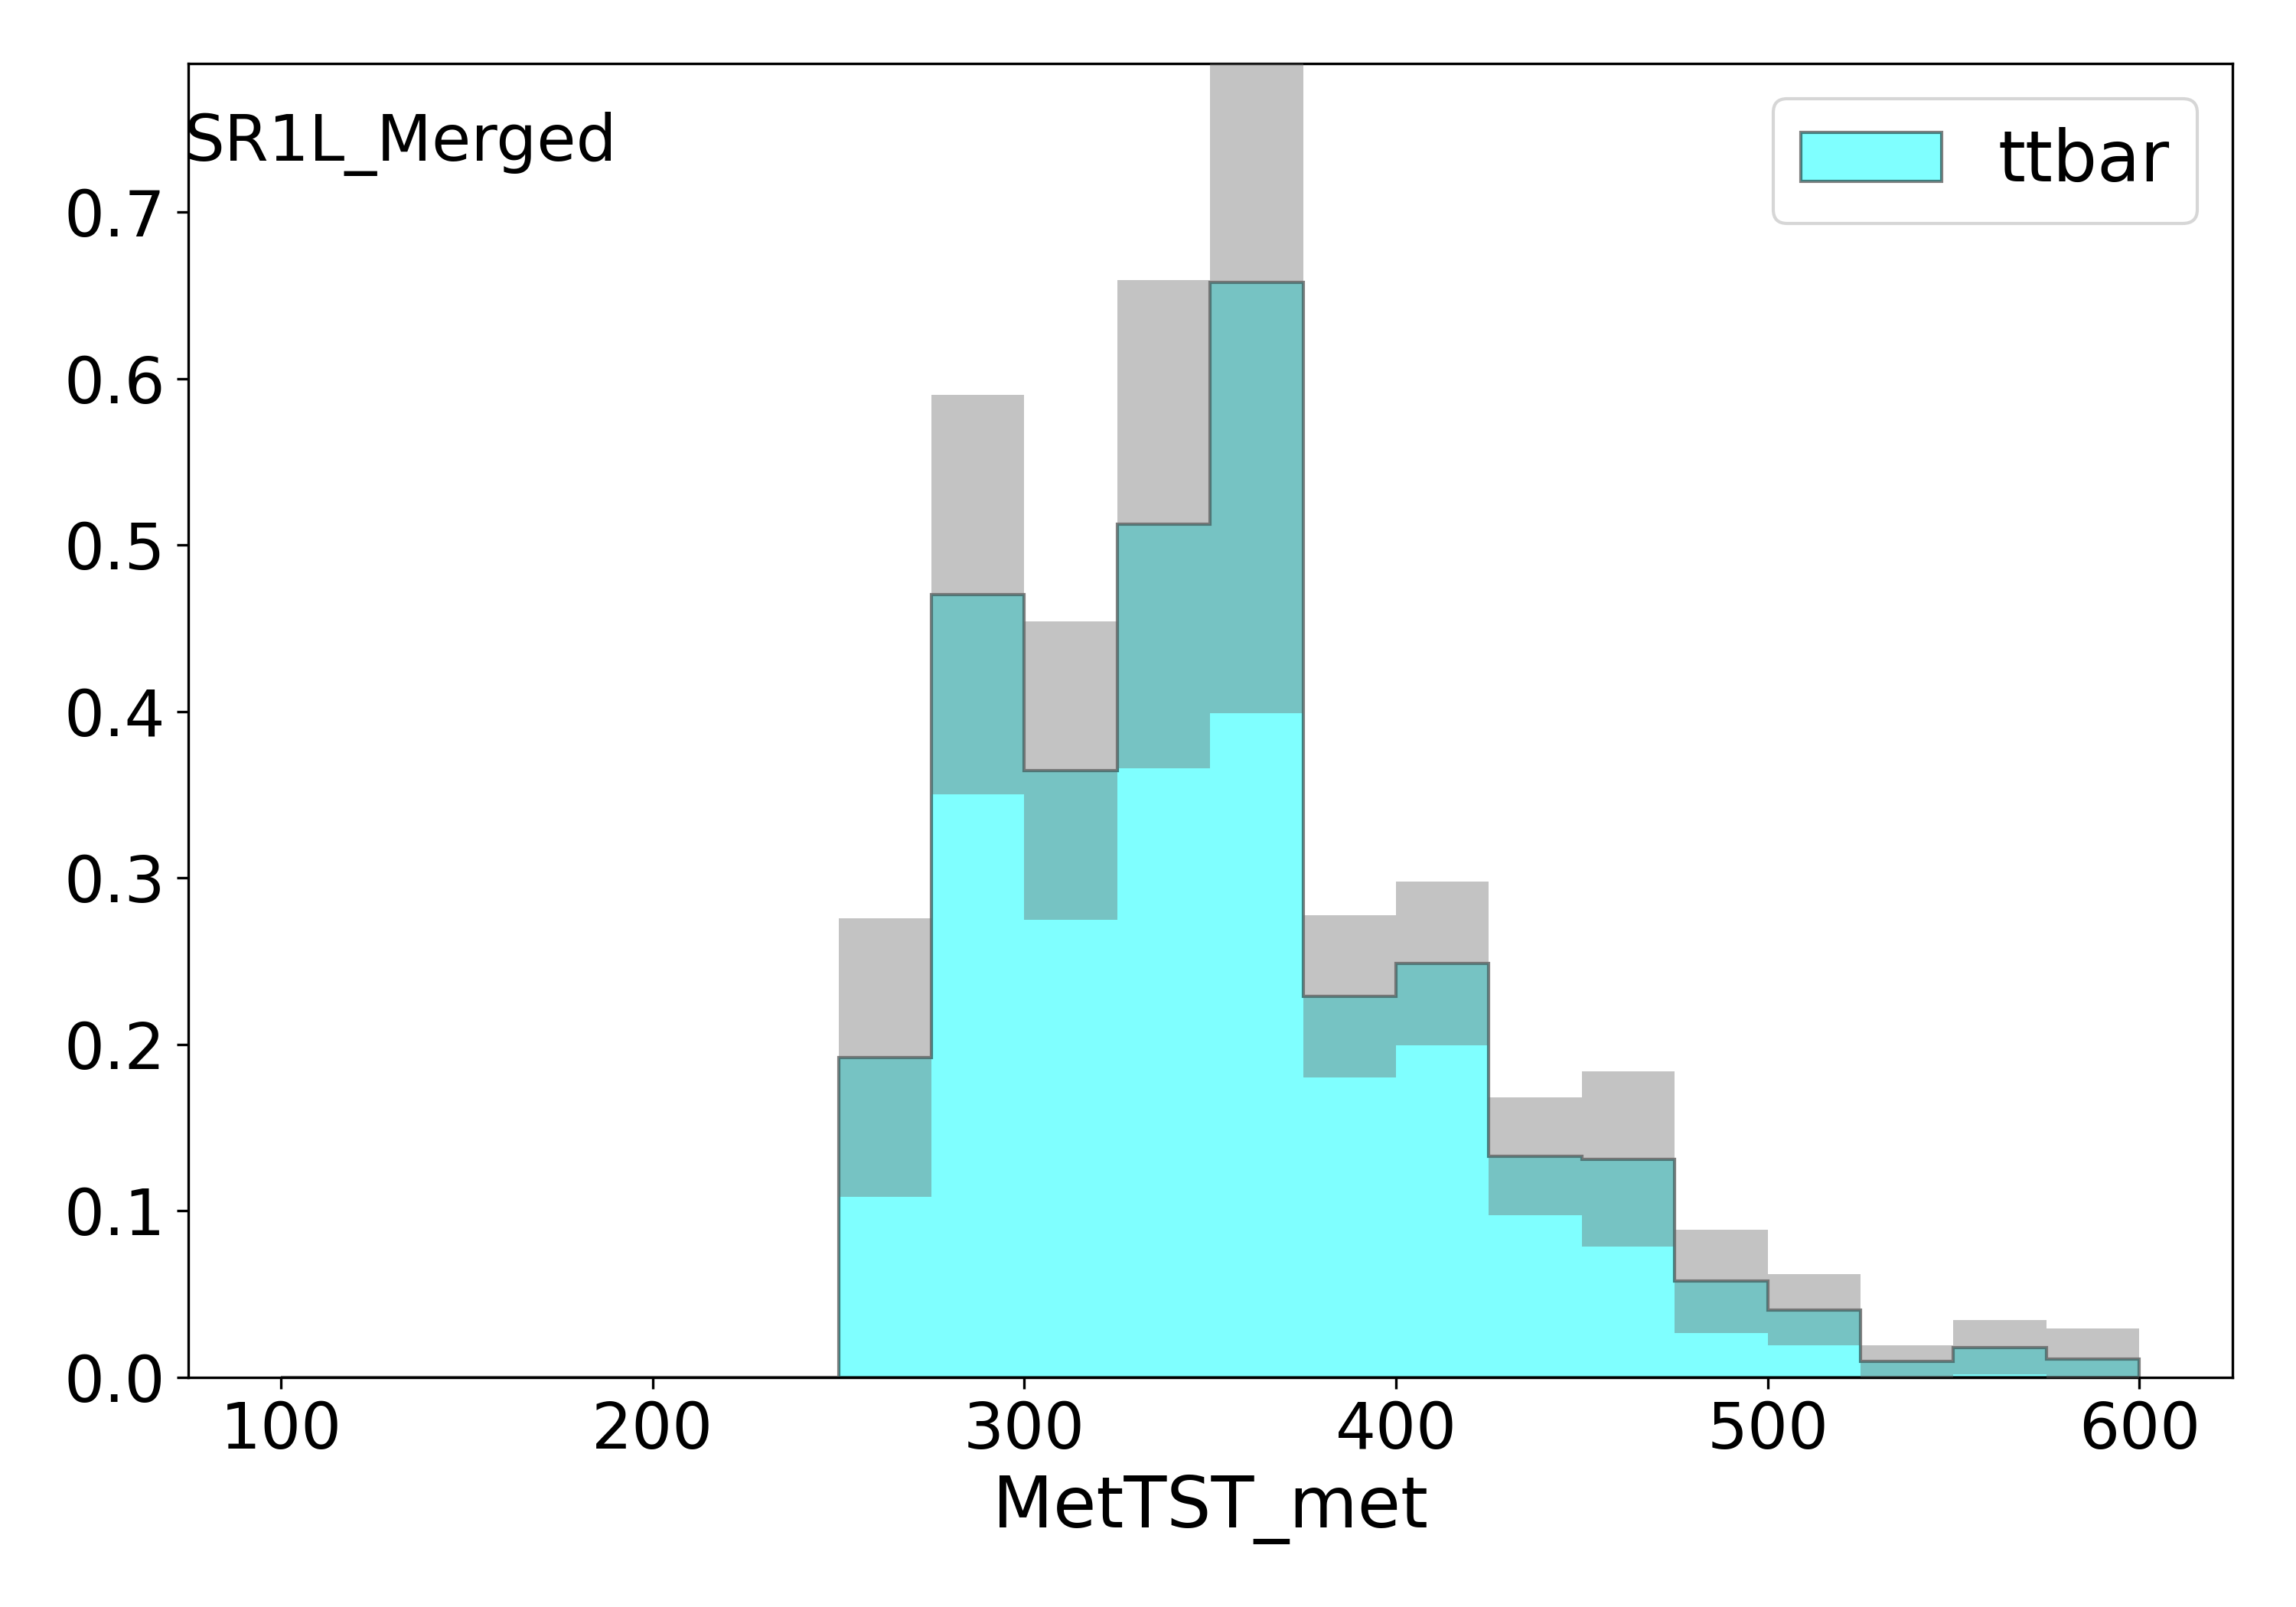
\includegraphics[width = 0.98\textwidth]{Figures/4/CRSR/SR1L_Merged/MetTST_met.png}
    \caption{Merged SR \met}
    \end{subfigure}
    \begin{subfigure}{0.49\textwidth}
    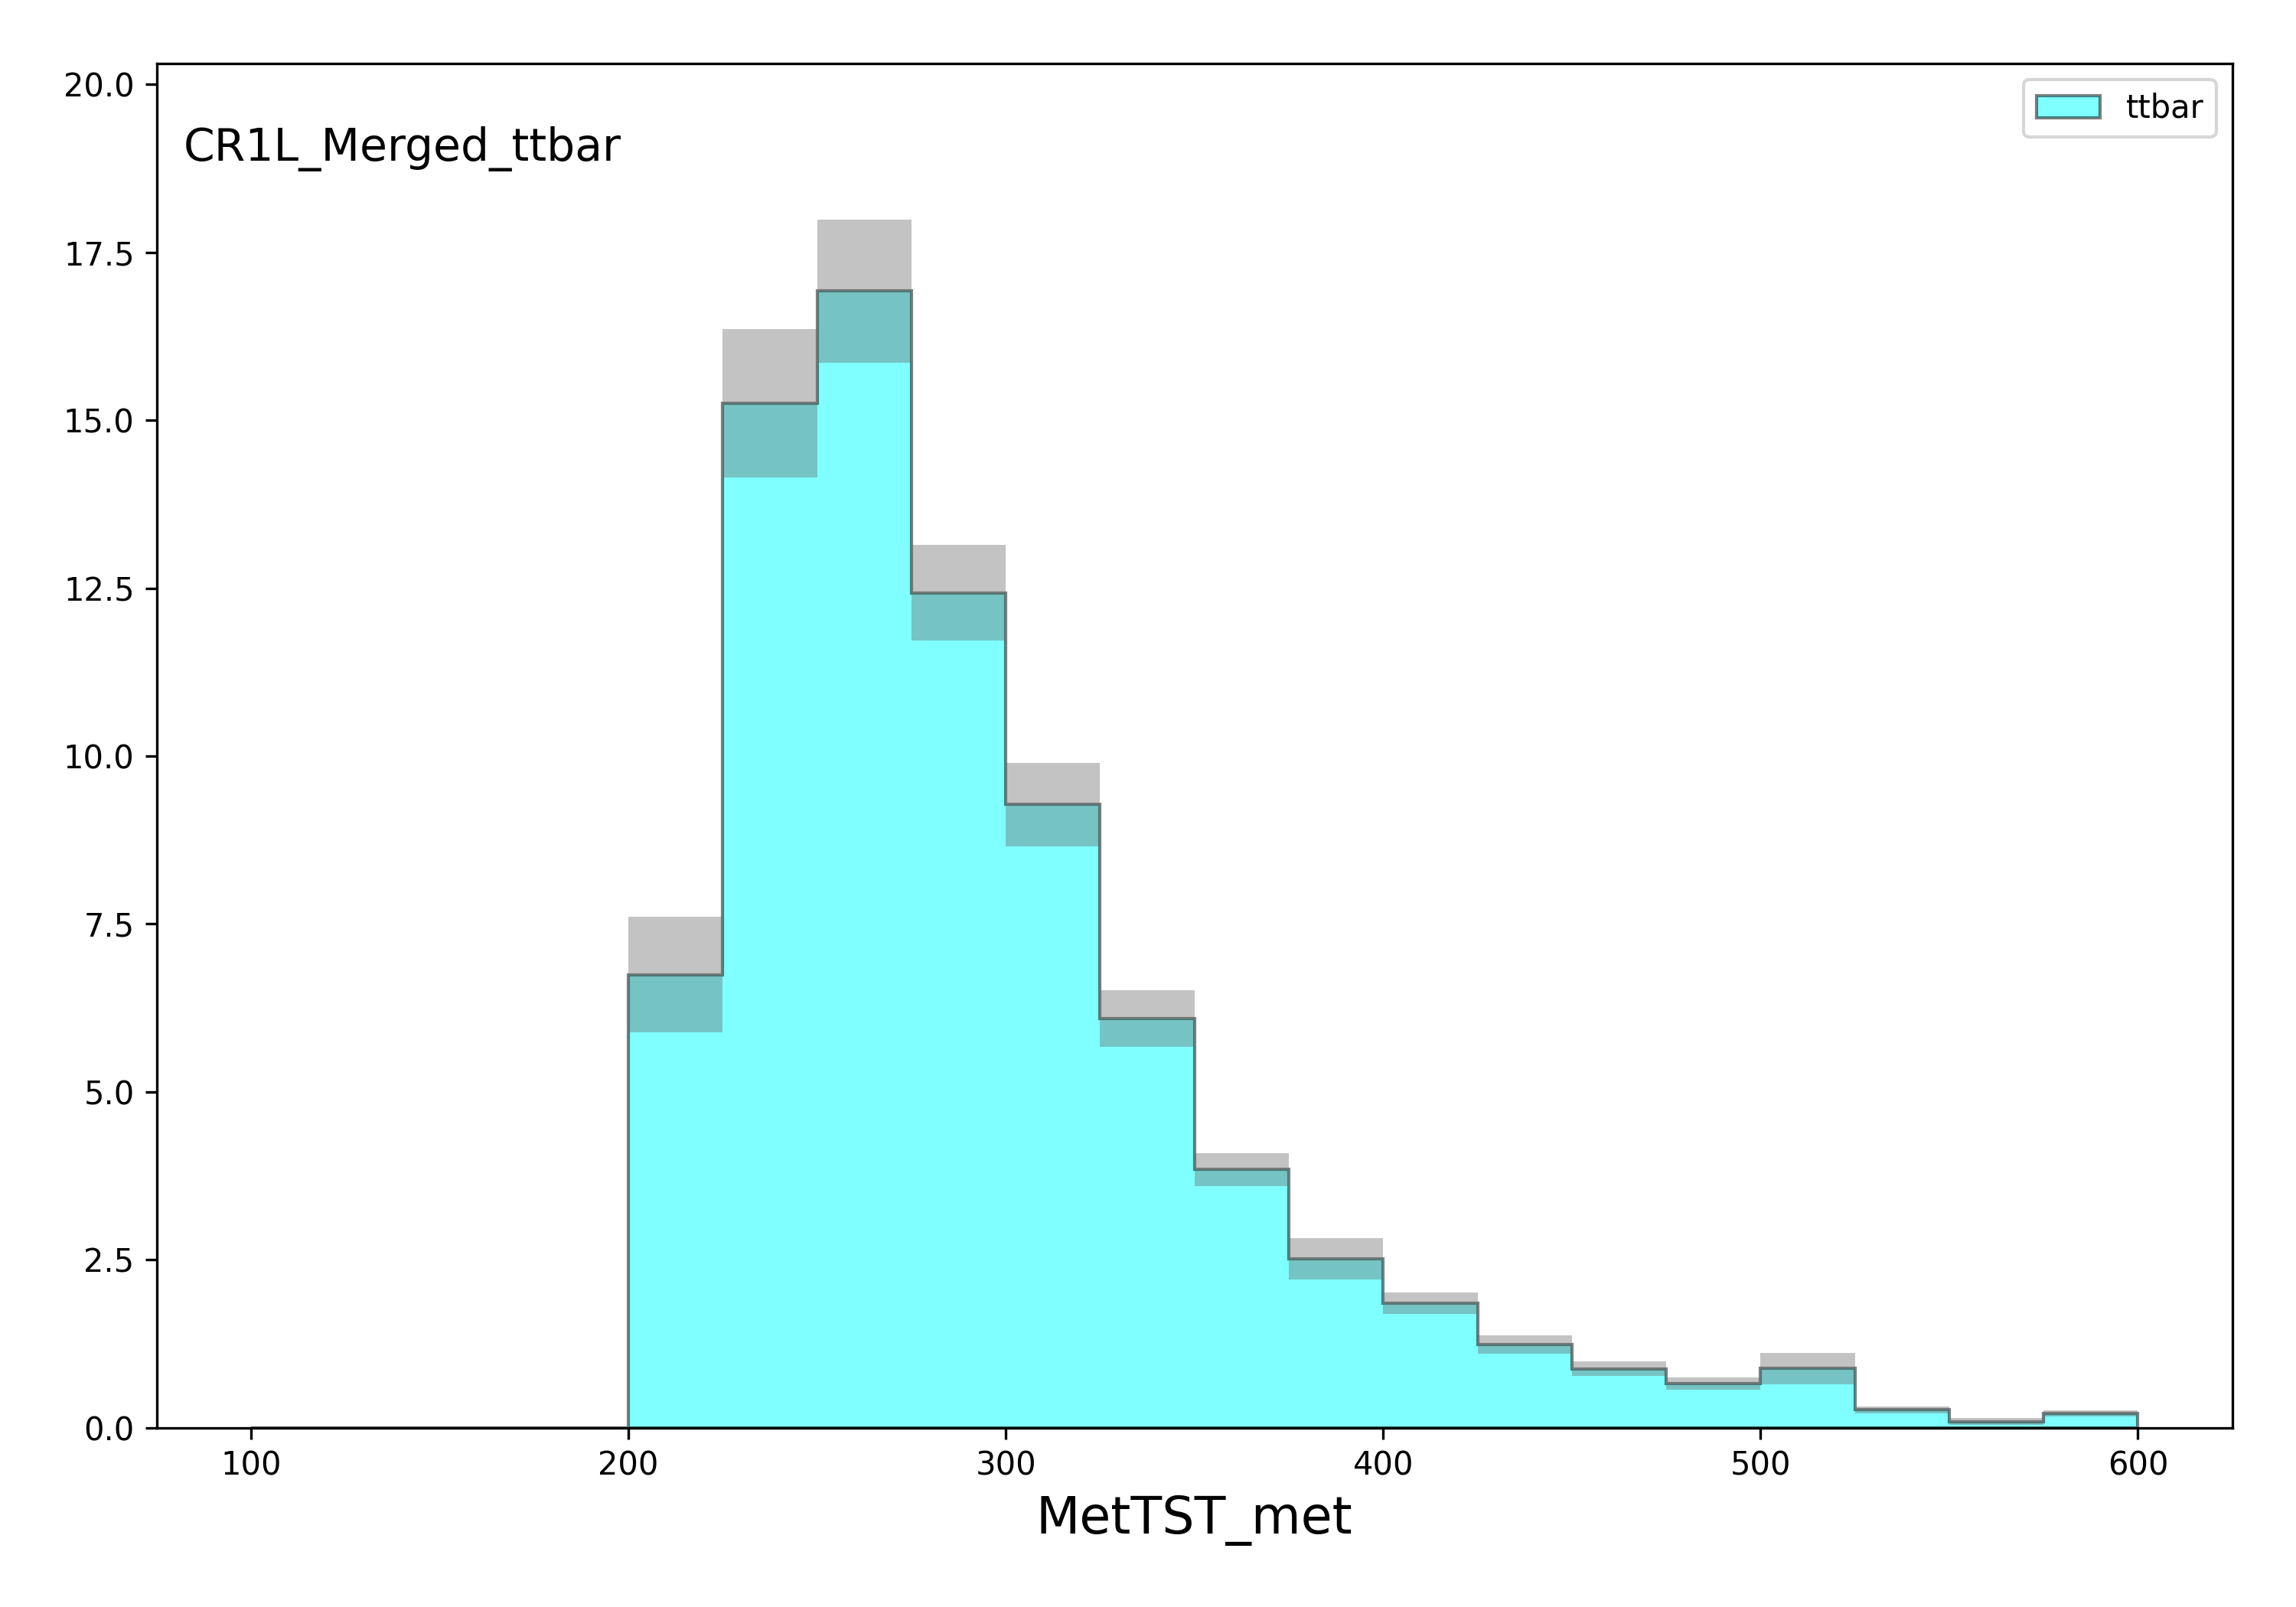
\includegraphics[width = 0.98\textwidth]{Figures/4/CRSR/CR1L_Merged_ttbar/MetTST_met.png}
    \caption{Merged CR \met}
    \end{subfigure}


     \caption{Comparisons of kinematic variables between the \merged signal region and \ttbar control region. \textbf{Left column:} signal region, \textbf{Right column:} control region. Grey bands represent MC statistical uncertainty on each bin.}
     \label{fig:CRSR_merged}
  \end{figure}

  \begin{figure}[htbp]
    \centering

      \begin{subfigure}{0.49\textwidth}
      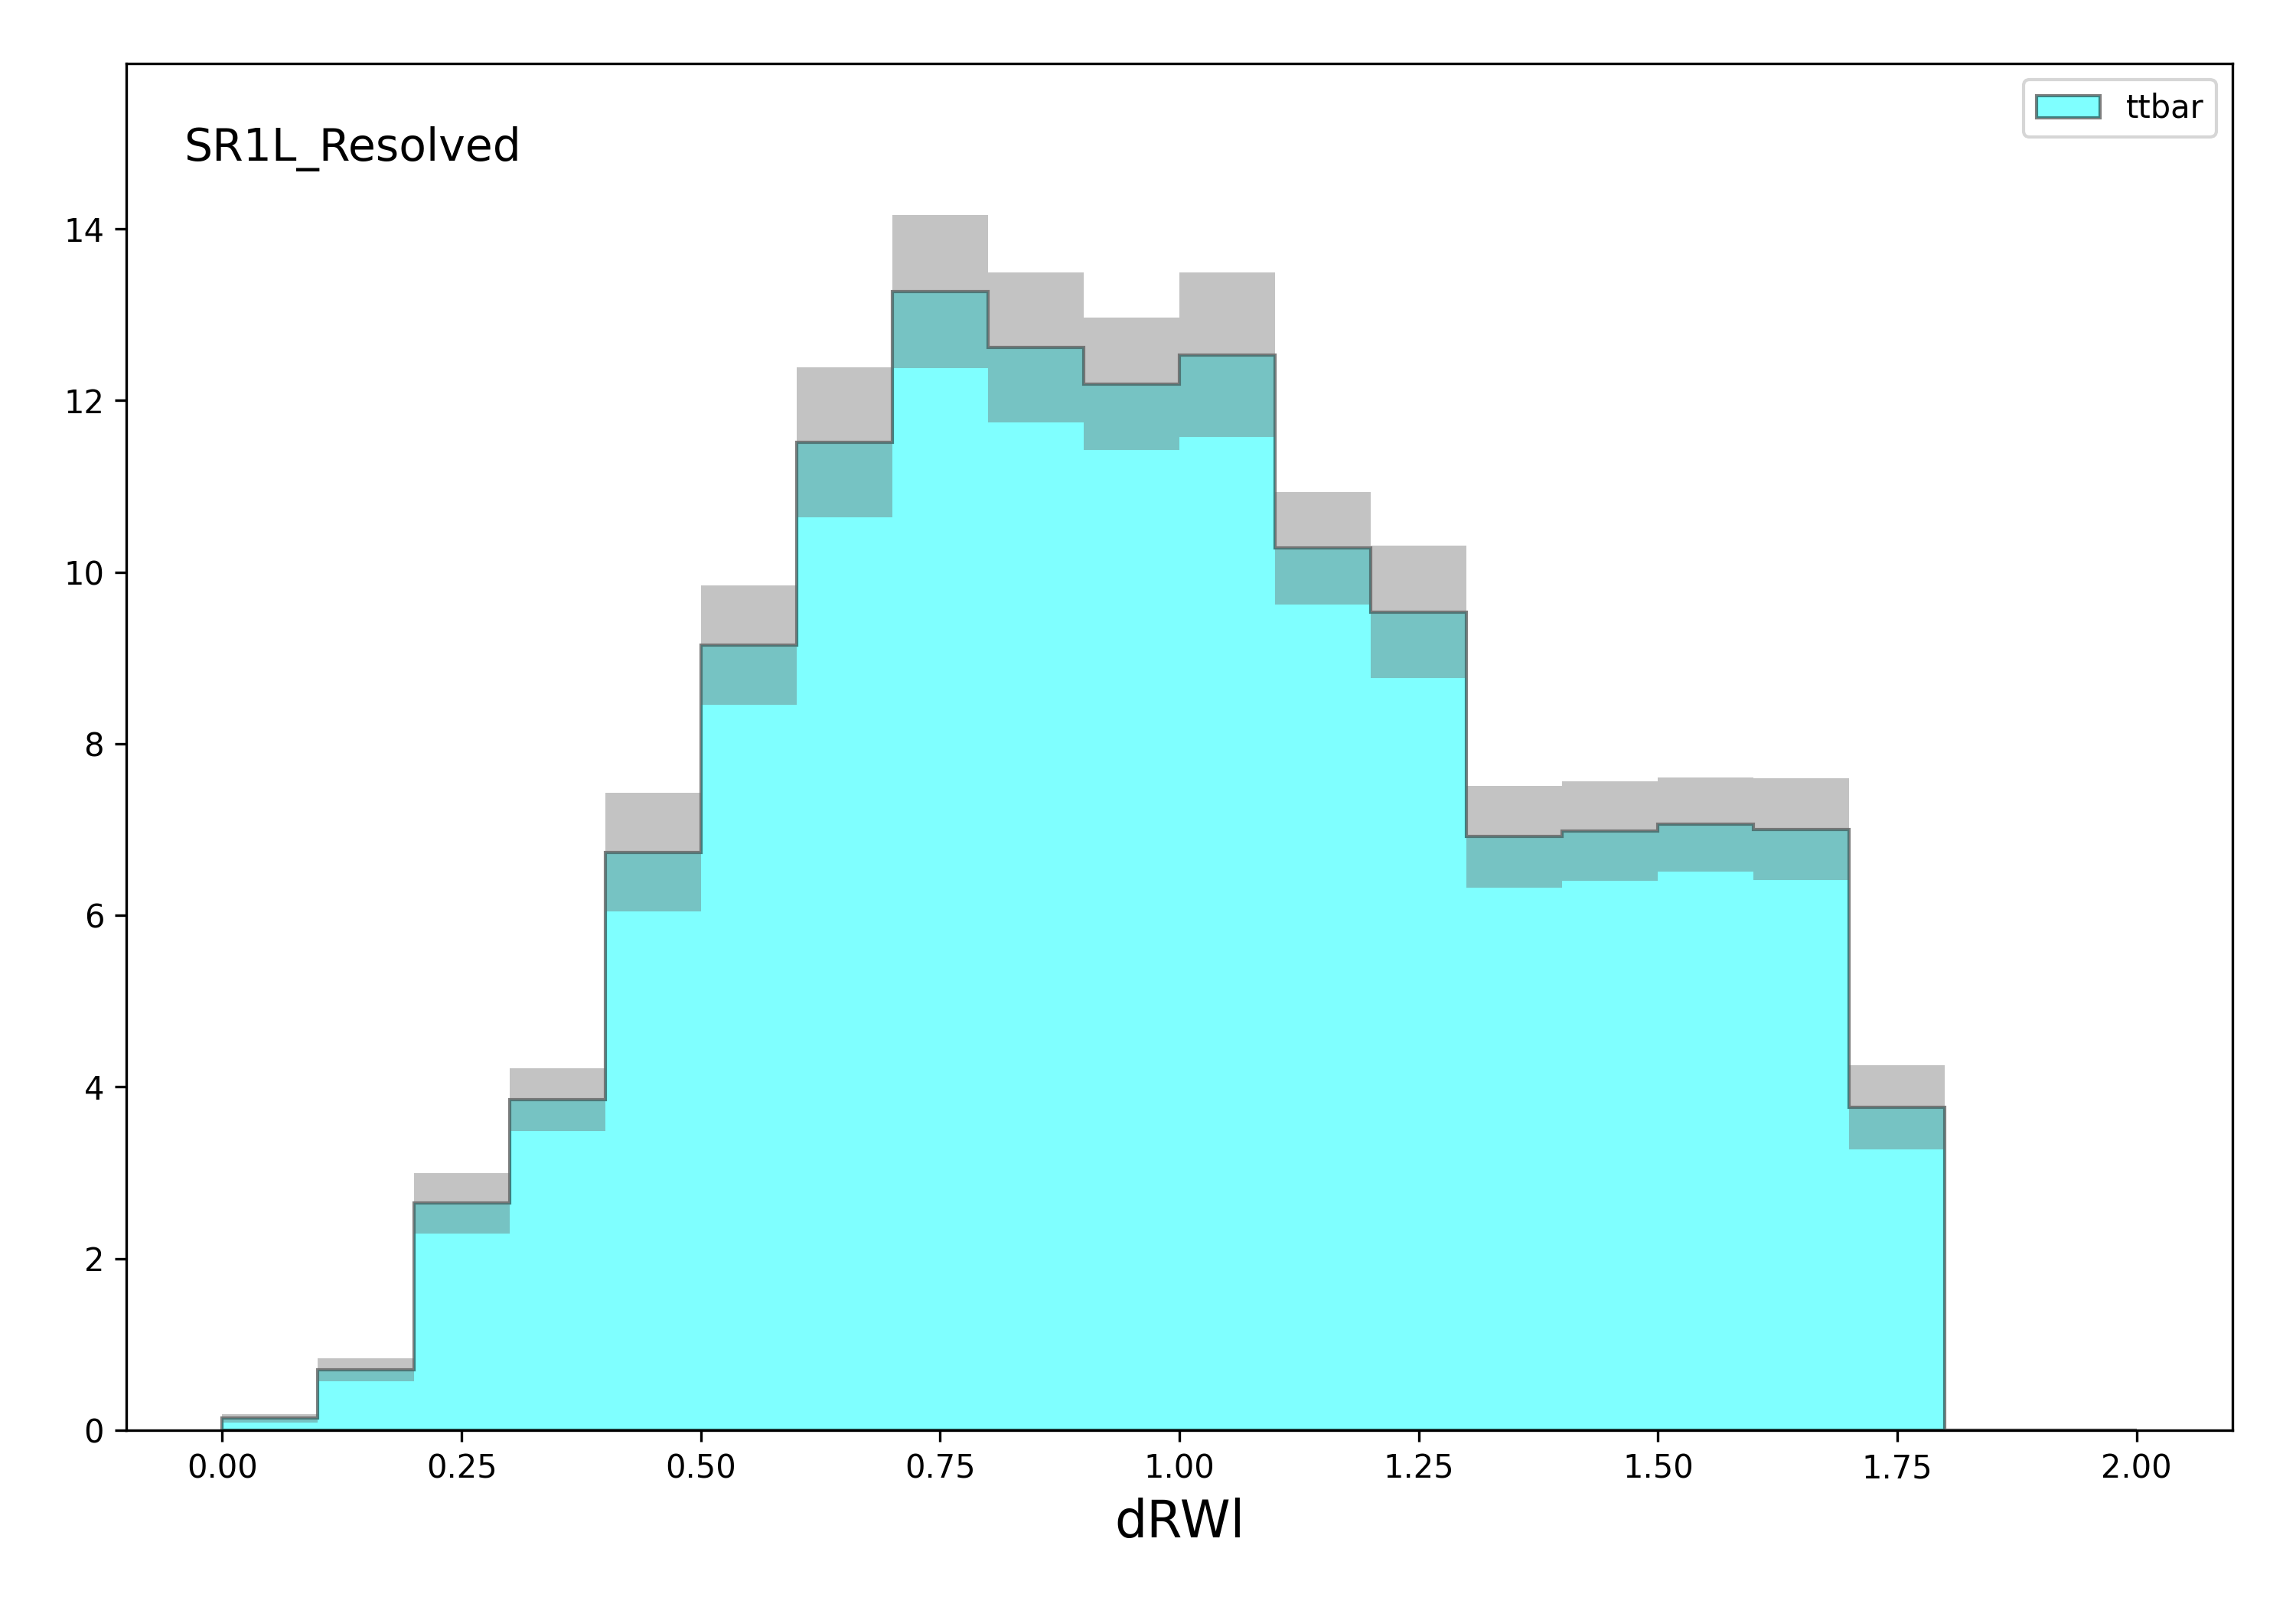
\includegraphics[width = 0.98\textwidth]{Figures/4/CRSR/SR1L_Resolved/dRWl.png}
      \caption{Resolved SR \drWl}
      \end{subfigure}
      \begin{subfigure}{0.49\textwidth}
      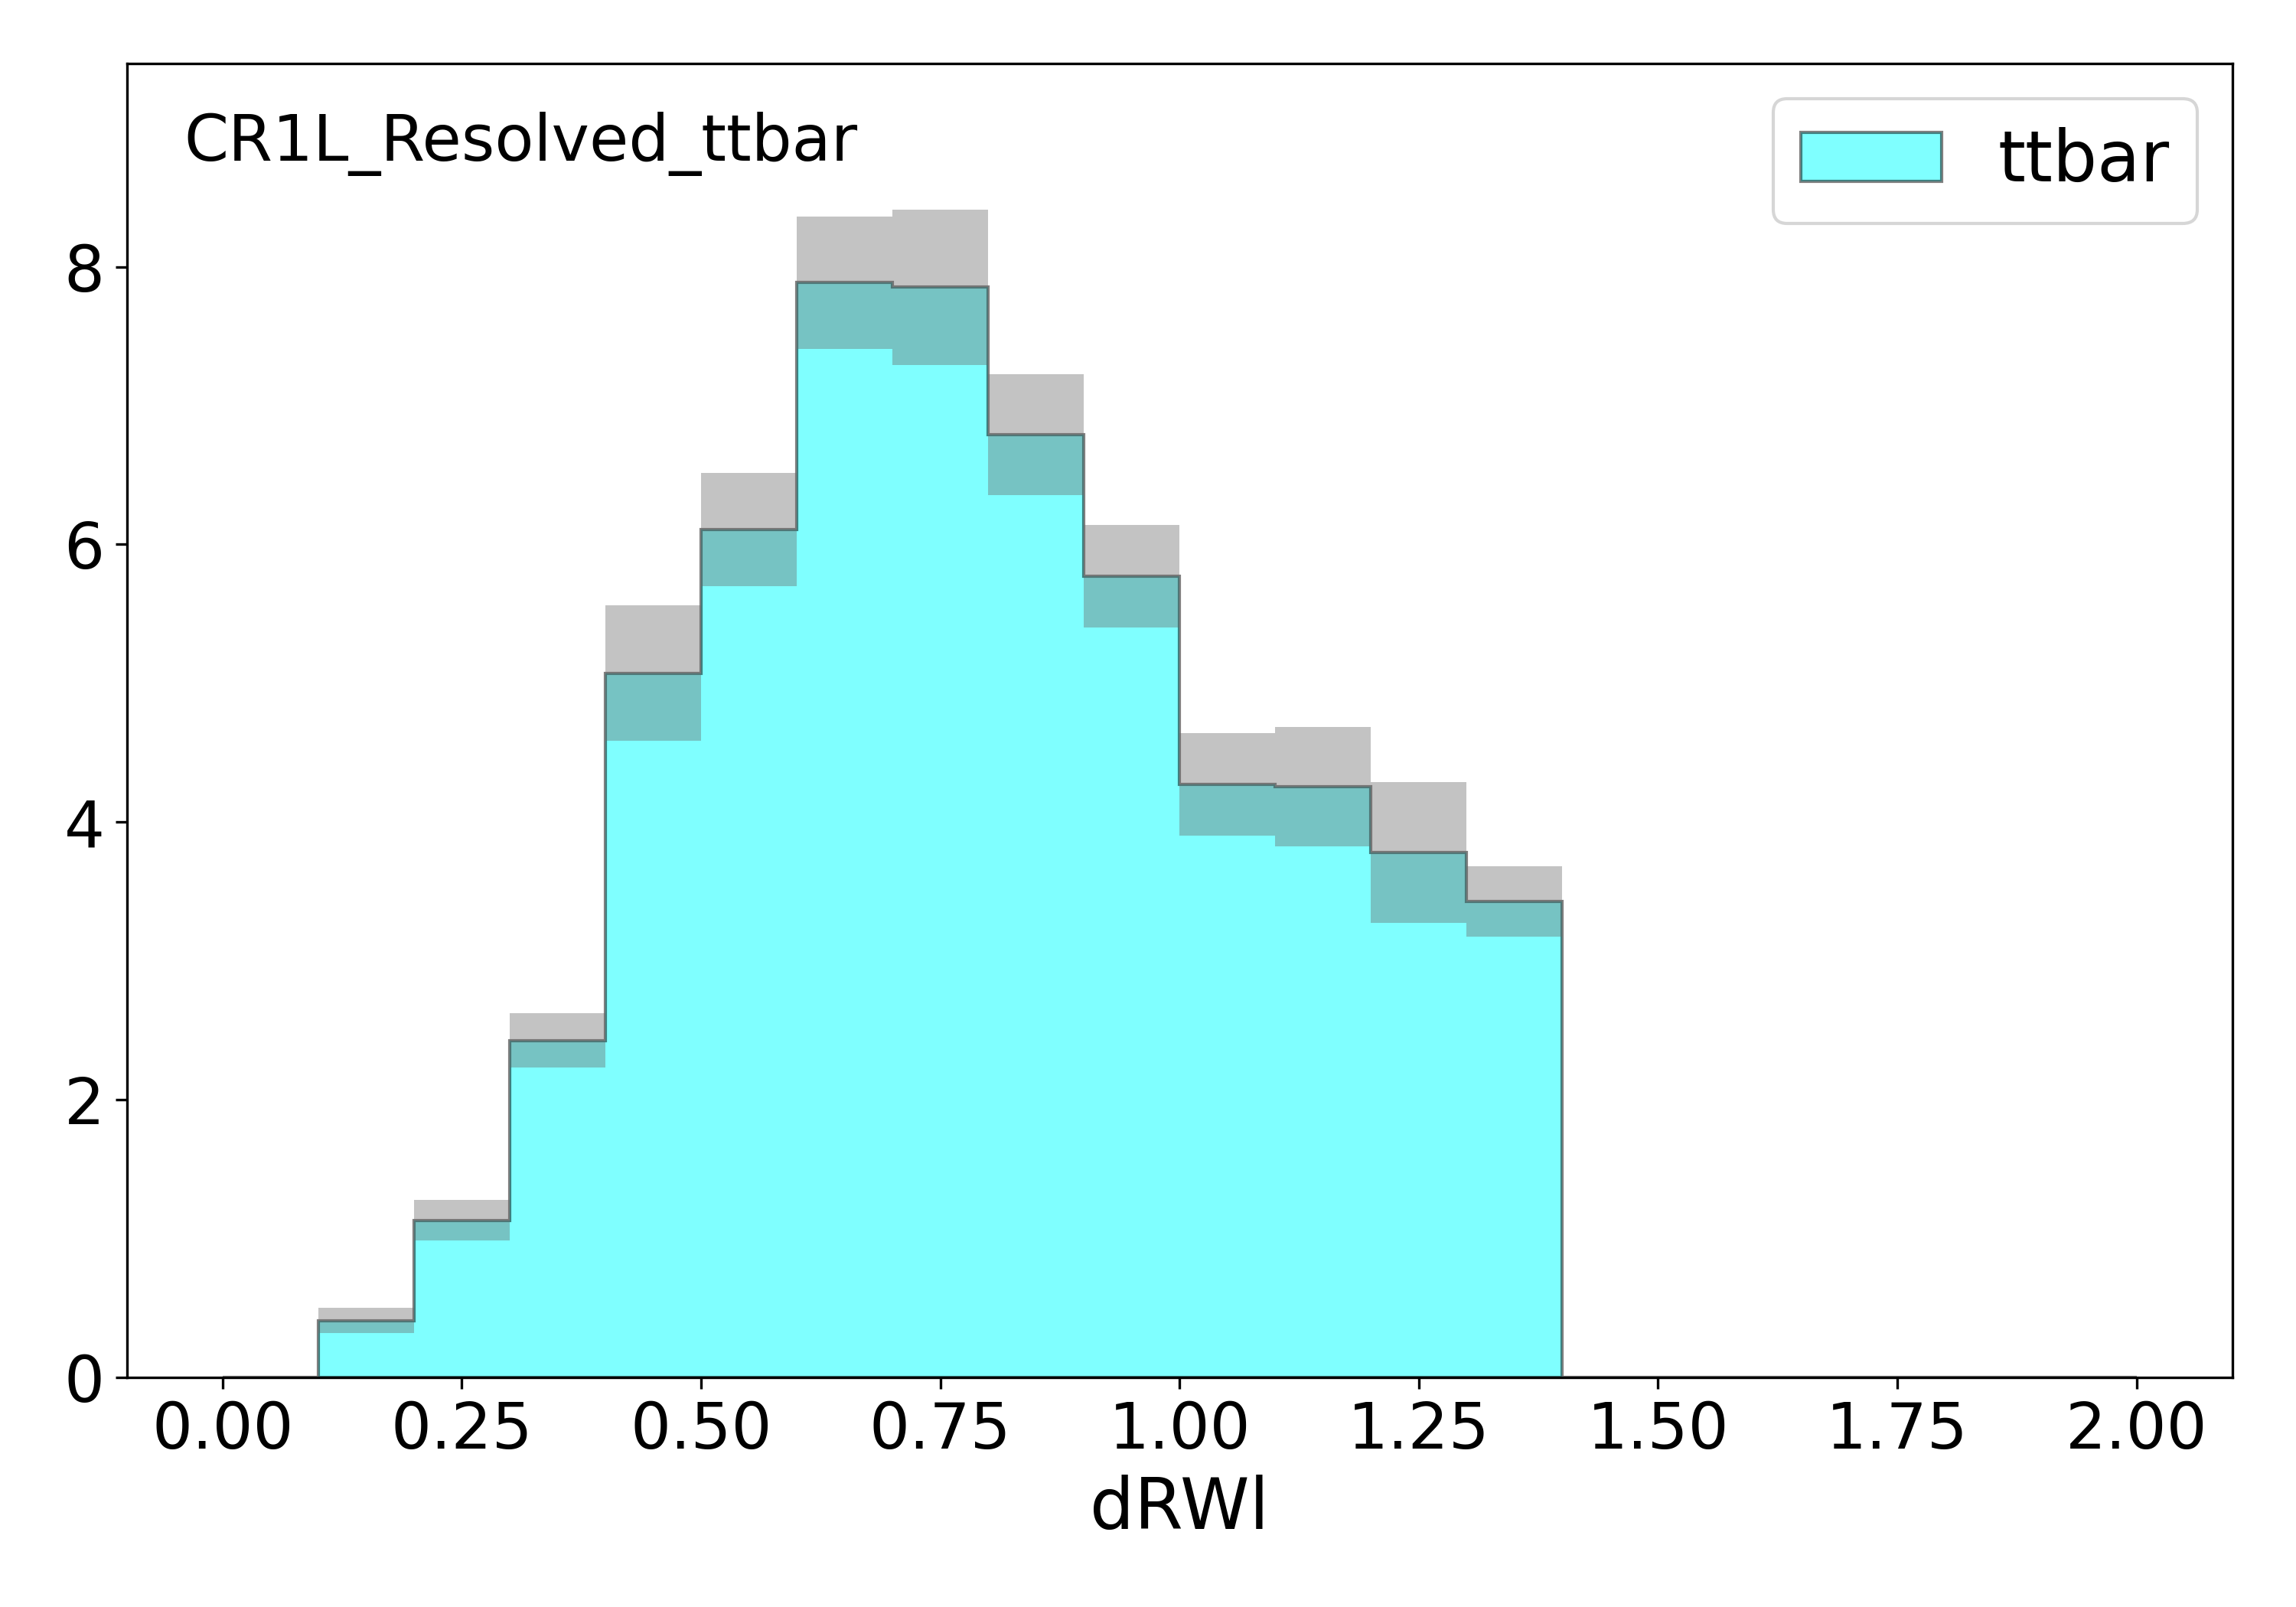
\includegraphics[width = 0.98\textwidth]{Figures/4/CRSR/CR1L_Resolved_ttbar/dRWl.png}
      \caption{Resolved CR \drWl}
      \end{subfigure}
      \begin{subfigure}{0.49\textwidth}
      \includegraphics[width = 0.98\textwidth]{Figures/4/CRSR/SR1L_Resolved/mT_lep_met.png}
      \caption{Resolved SR \mtlepmet}
      \end{subfigure}
      \begin{subfigure}{0.49\textwidth}
      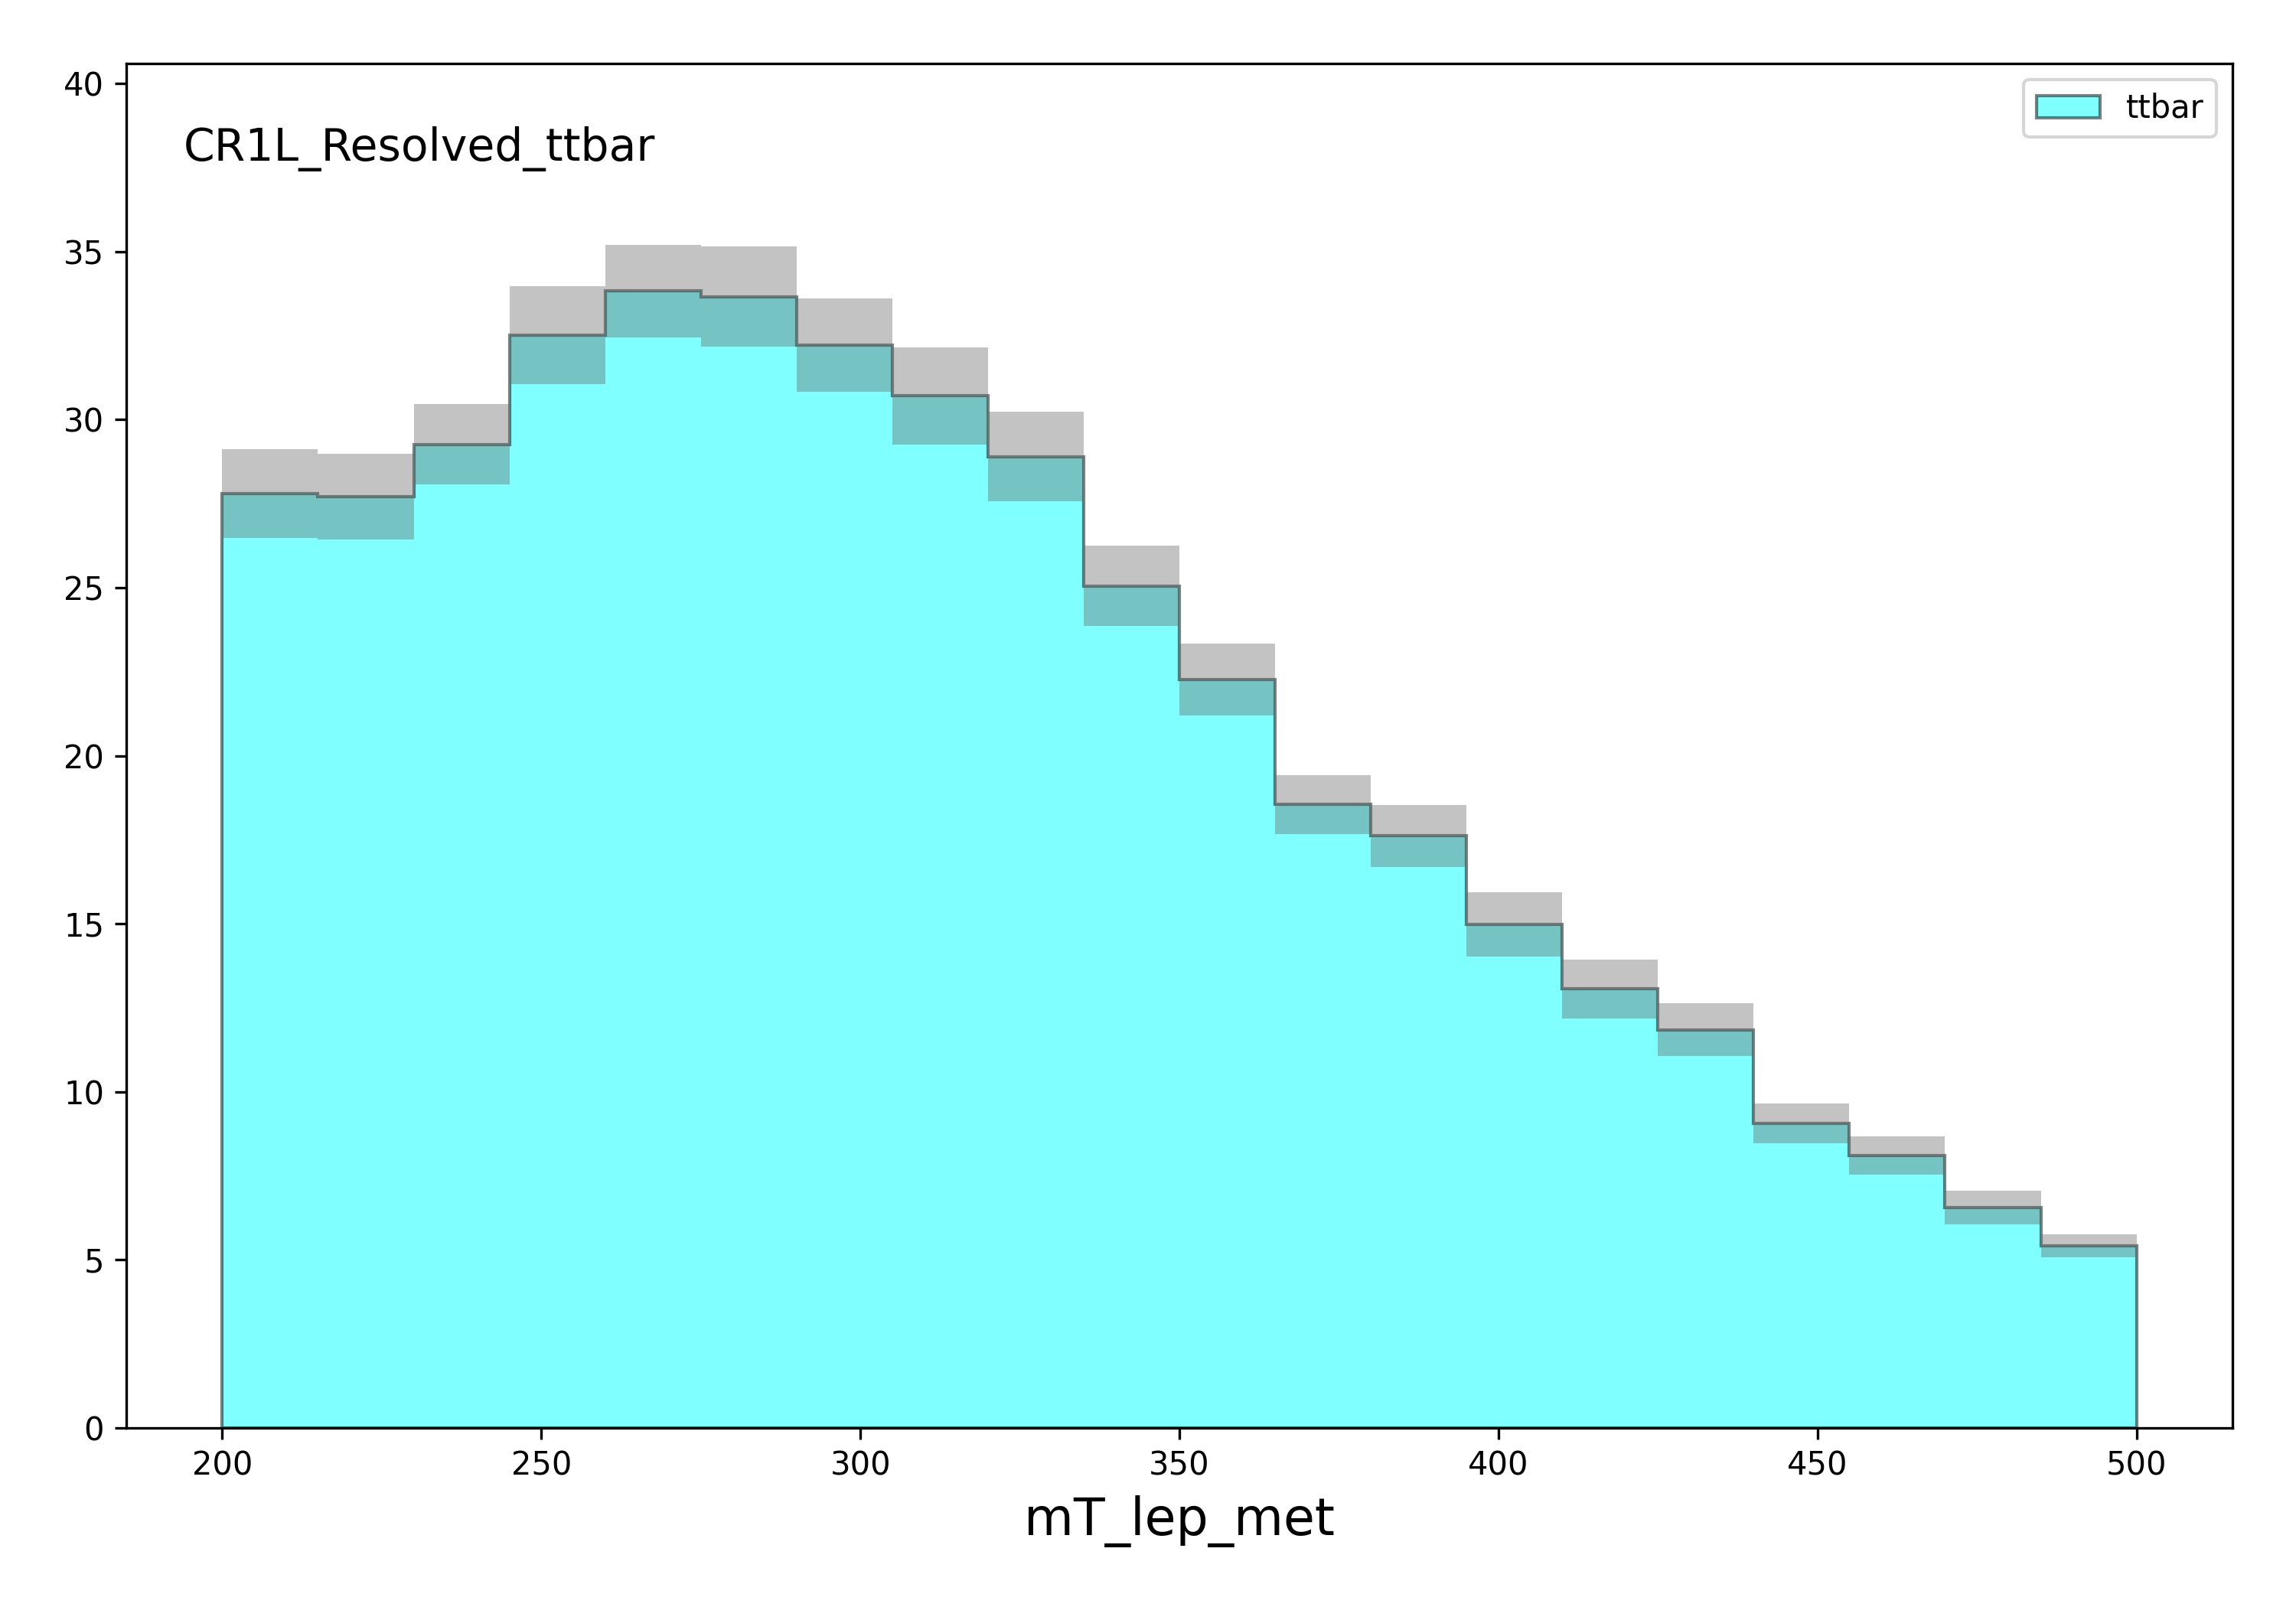
\includegraphics[width = 0.98\textwidth]{Figures/4/CRSR/CR1L_Resolved_ttbar/mT_lep_met.png}
      \caption{Resolved CR \mtlepmet}
      \end{subfigure}
      \caption{Comparisons of kinematic variables between the \resolved signal region and \ttbar control region. \textbf{Left column:} signal region, \textbf{Right column:} control region. Grey bands represent MC statistical uncertainty on each bin.}
      \label{fig:CRSR_resolved}
   \end{figure}
   \begin{figure}[htbp]
     \centering
      \begin{subfigure}{0.49\textwidth}
      \includegraphics[width = 0.98\textwidth]{Figures/4/CRSR/SR1L_Resolved/MetTST_met.png}
      \caption{Resolved SR \met}
      \end{subfigure}
      \begin{subfigure}{0.49\textwidth}
      \includegraphics[width = 0.98\textwidth]{Figures/4/CRSR/CR1L_Resolved_ttbar/MetTST_met.png}
      \caption{Resolved CR \met}
      \end{subfigure}


       \caption{Comparisons of kinematic variables between the \resolved signal region and \ttbar control region. \textbf{Left column:} signal region, \textbf{Right column:} control region. Grey bands represent MC statistical uncertainty on each bin.}
       \label{fig:CRSR_resolved}
    \end{figure}

\FloatBarrier
\section{$N-1$ Plots - Highly Weighted Event Included}
\label{section:N1_backup}
The following section contains $N-1$ plots in the ``merged" signal region, with the inlcusion of the single highly negatively weighted event excluded in Section \ref{section:sr_merged}.
\begin{figure}[htbp]
  \centering

     \begin{subfigure}{0.49\textwidth}
     \includegraphics[width = 0.98\textwidth]{Figures/4/N1n/mT_lep_met.pdf}
     \caption{\mtlepmet}
     \end{subfigure}
     \begin{subfigure}{0.49\textwidth}
     \includegraphics[width = 0.98\textwidth]{Figures/4/N1n/MetTST_Significance.pdf}
     \caption{\metsig}
     \end{subfigure}
     \begin{subfigure}{0.49\textwidth}
     \includegraphics[width = 0.98\textwidth]{Figures/4/N1n/dR_lep_TARJets10.pdf}
     \caption{\drTARl}
     \end{subfigure}
     \begin{subfigure}{0.49\textwidth}
     \includegraphics[width = 0.98\textwidth]{Figures/4/N1n/TARJets10_TAR_D20.pdf}
     \caption{\DtwoTAR}
     \end{subfigure}
     \caption{$N-1$ plots in the \merged signal region with the inclusion of a highly negatively weighted background event. Grey bands represent MC statistical uncertainty on each bin.}
     \label{fig:SRN1_backup}
  \end{figure}
  \begin{figure}[htbp]
    \centering
     \begin{subfigure}{0.49\textwidth}
     \includegraphics[width = 0.98\textwidth]{Figures/4/N1n/TARJets10_mTAR0.pdf}
     \caption{\mTAR}
     \end{subfigure}
     \begin{subfigure}{0.49\textwidth}
     \includegraphics[width = 0.98\textwidth]{Figures/4/N1n/TARJets10_mTAR02.pdf}
     \caption{\mTAR}
     \end{subfigure}

     \caption{$N-1$ plots in the \merged signal region with the inclusion of a highly negatively weighted background event. Grey bands represent MC statistical uncertainty on each bin.}
     \label{fig:SRN1_backup}
  \end{figure}
\FloatBarrier
